\documentclass[a4paper]{article}
\usepackage[T1]{fontenc}			% pacchetto per \chapter
\usepackage[italian]{babel}
\usepackage[italian]{isodate}  		% formato delle date in italiano
\usepackage{graphicx}				% gestione delle immagini
\usepackage{amsfonts}
\usepackage{booktabs}				% tabelle di qualità superiore
\usepackage{amsmath}				% pacchetto matematica
\usepackage{amsthm}					% teoremi migliorati (QED)
\usepackage{mathtools}				% pacchetto matematica pt.2
\usepackage{amssymb}				% pacchetto matematica pt.3
\usepackage{stmaryrd} 				% per '\llbracket' e '\rrbracket'
\usepackage{enumitem}				% gestione delle liste
\usepackage{pifont}					% pacchetto con elenchi carini
\usepackage{listings}				% pacchetto per i codici
\usepackage[x11names]{xcolor}		% pacchetto colori RGB
\usepackage{tcolorbox}				% pacchetto per le box colorate
\usepackage{cancel}					% per le approssimazioni (e.g. cancelto)
% Link ipertestuali per l'indice
\usepackage{xcolor}
\usepackage[linkcolor=black, citecolor=blue, urlcolor=cyan]{hyperref}
\hypersetup{
	colorlinks=true
}

\newcommand{\longline}{\noindent\rule{\textwidth}{0.4pt}}
\newcommand{\exec}[1]{\left\llbracket #1\:\right\rrbracket}
\renewcommand{\qedsymbol}{QED}

\definecolor{codegreen}{rgb}{0,0.6,0}
\definecolor{codegray}{rgb}{0.5,0.5,0.5}
\definecolor{codepurple}{rgb}{0.58,0,0.82}
\definecolor{backcolour}{rgb}{0.95,0.95,0.92}
\lstdefinestyle{mystyle}{
	backgroundcolor=\color{backcolour},   
	commentstyle=\color{codegreen},
	keywordstyle=\color{magenta},
	numberstyle=\tiny\color{codegray},
	stringstyle=\color{codepurple},
	basicstyle=\ttfamily\footnotesize,
	breakatwhitespace=false,         
	breaklines=true,                 
	captionpos=b,                    
	keepspaces=true,                 
	numbers=left,                    
	numbersep=5pt,                  
	showspaces=false,                
	showstringspaces=false,
	showtabs=false,                  
	tabsize=2
}

\lstdefinelanguage{JavaScript}{
	keywords={typeof, new, true, false, catch, function, return, null, catch, switch, var, if, in, while, do, else, case, break},
	keywordstyle=\color{blue}\bfseries,
	ndkeywords={class, export, boolean, throw, implements, import, this},
	ndkeywordstyle=\color{darkgray}\bfseries,
	identifierstyle=\color{black},
	sensitive=false,
	comment=[l]{//},
	morecomment=[s]{/*}{*/},
	commentstyle=\color{codegreen}\ttfamily,
	stringstyle=\color{red}\ttfamily,
	morestring=[b]',
	morestring=[b]"
}

\lstset{
	language=JavaScript,
	backgroundcolor=\color{lightgray},
	extendedchars=true,
	basicstyle=\footnotesize\ttfamily,
	showstringspaces=false,
	showspaces=false,
	numbers=left,
	numberstyle=\footnotesize,
	numbersep=9pt,
	tabsize=2,
	breaklines=true,
	showtabs=false,
	captionpos=b
}

\lstset{style=mystyle}

%\usepackage{showframe}				% visualizzazione bordi
%\usepackage{showkeys}				% visualizzazione etichetta

\newcommand{\dquotes}[1]{``#1''}

\begin{document}
	\newcounter{definition}[section]
	\newtcolorbox{boxdef}{colback=red!5!white,colframe=red!75!black,fonttitle=\bfseries,title=Definizione~\refstepcounter{definition}\thedefinition}
	
%	\newenvironment{definition}[1][]{\begin{center}\begin{tabular}{|p{\textwidth}|}\hline%
%				\refstepcounter{definition}\par\medskip
%		\noindent \textcolor{Red3}{\textbf{Definizione~\thedefinition. #1}} \rmfamily}{\medskip%
%		\\\hline
%		\end{tabular} 
%		\end{center}}
	
	\author{VR443470}
	\title{Linguaggi}
	\date{\printdayoff\today}
	\maketitle
	
	\newpage
	
	% indice
	\tableofcontents
	
	\newpage
	
	\section{Introduzione}
	
	\subsection{Nascita dei linguaggi}
	
	Il problema \textbf{principale dell'informatica} consiste nel voler far eseguire ad una macchina \textbf{algoritmi} che manipolano \textbf{dati}. Con il termine \dquotes{macchina} si intende un dispositivo \textbf{programmabile}, ovvero un calcolatore, che può eseguire un insieme di istruzioni chiamate programmi, ricevuti come input (\textcolor{Red3}{\textbf{macchine universali}}).\newline
	
	\noindent
	In particolare, i computer moderni hanno un'architettura che nasce da quella di Von Neumann.
	\begin{figure}[!htp]
		\centering
		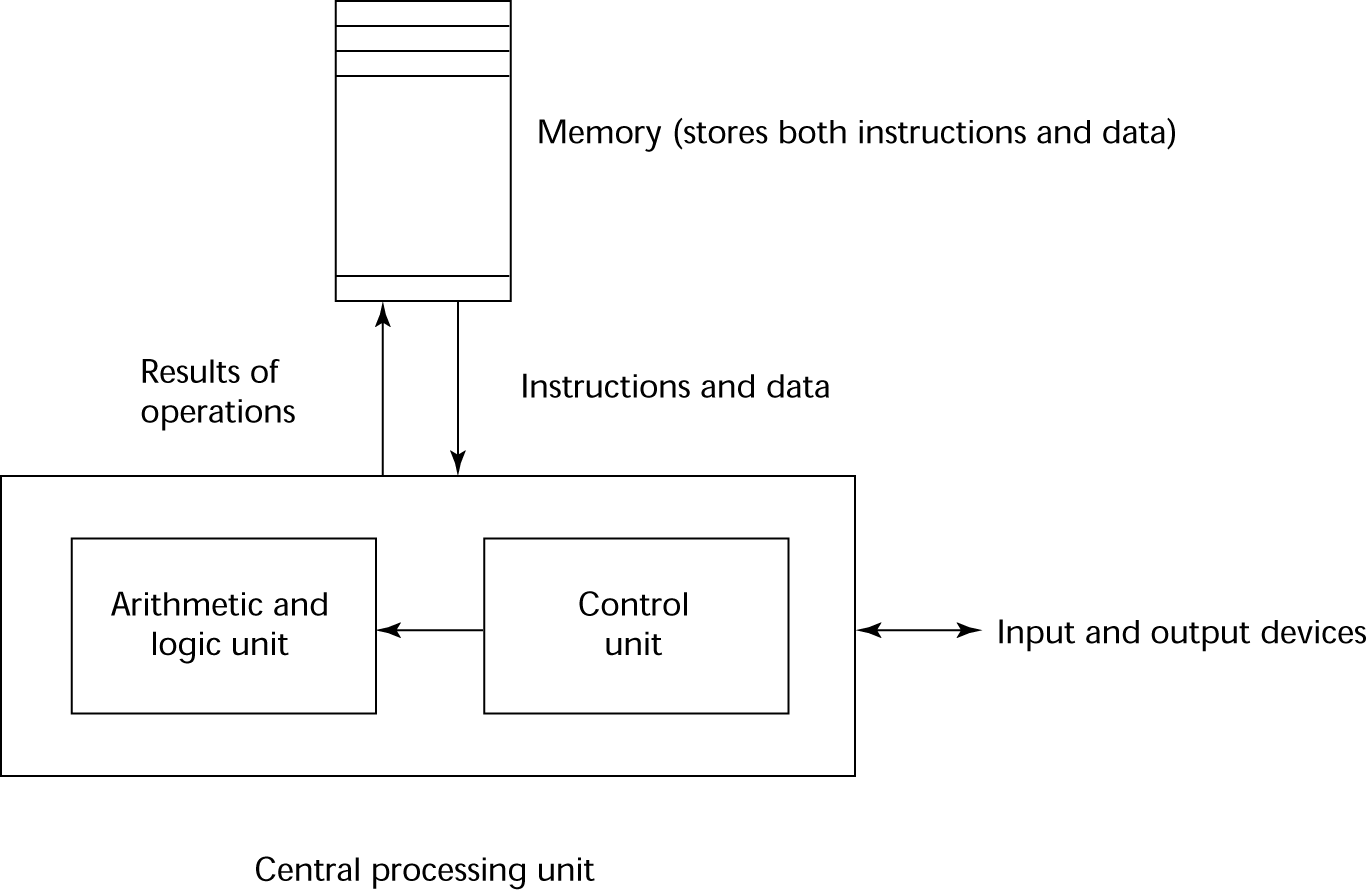
\includegraphics[width=\textwidth]{img/von_neumann.png}
		\caption{Architettura di Von Neumann.}
	\end{figure}

	\noindent
	Per operare su tali macchine, fu necessario inserire una CPU per eseguire algoritmi e operare sui dati in memoria. Il primo linguaggio che consente di programmare tale architettura è quello basato sull'implementazione dell'architettura stessa, ovvero la programmazione con schede perforate per esempio.\newpage
	
	\subsection{Definizioni}
	
	\subsubsection{Algoritmo}
	
	\begin{boxdef}
		Un \textcolor{Red3}{\textbf{algoritmo}} \textbf{è una sequenza finita di passi primitivi di calcolo descritti mediante una frase ben formata (programma) in un linguaggio di programmazione}.
	\end{boxdef}

	\noindent
	In altre parole, un algoritmo scompone un calcolo complesso in passi elementari di computazione. Esso è dunque un concetto astratto che trova la sua forma concreta in un programma che è la sequenza finita di istruzioni.\newline
	Data la definizione, è necessario precisare che:
	\begin{itemize}
		\item \textbf{Un programma non è necessariamente un algoritmo}, poiché una frase grammaticalmente corretta potrebbe non avere significato;
		\item \textbf{Lo stesso algoritmo può avere concretizzazioni diverse}, ovvero lo stesso algoritmo può essere implementato da infiniti programmi.
	\end{itemize}

	\longline

	\subsubsection{Dati}

	I programmi sono la concretizzazione degli algoritmi, i quali manipolano i \textcolor{Red3}{\textbf{dati}}. Essi sono informazioni memorizzate sia concretamente in celle di memoria, sia astrattamente in elementi che il linguaggio di programmazione può manipolare, ovvero le \textbf{variabili}.
	
	\longline
	
	\subsubsection{Sintassi e semantica}

	La trasformazione (scrittura) di un programma in un determinato linguaggio di programmazione rappresenta la \textcolor{Red3}{\textbf{sintassi}}, mentre l'effetto della sua esecuzione e la trasformazione dei dati eseguita, costituisce la \textcolor{Red3}{\textbf{semantica}}.\newpage
	
	\subsubsection{Linguaggio matematico e logico}
	
	Il \textcolor{Red3}{\textbf{linguaggio matematico}} è una notazione rigorosa per rappresentare funzioni, ma non sempre oggetti infiniti e computazioni, cioè passi di calcolo.\newline
	
	\noindent
	Il \textcolor{Red3}{\textbf{linguaggio logico}} sono regole e assiomi che rendono possibile specificare il processo di computazione, in modo implicito, e consente di rappresentare formalmente oggetti infiniti in modo finito, ma non computazioni infinite.
	
	\longline
	
	\subsubsection{Linguaggio di programmazione}
	
	\begin{boxdef}
		Un \textcolor{Red3}{\textbf{linguaggio di programmazione}} consente di specificare in modo accurato esattamente le primitive del processo di computazione, con la rigorosità e la potenza della logica.
	\end{boxdef}

	\longline
	
	\subsubsection{Programma}
	
	Un \textcolor{Red3}{\textbf{programma}} è un insieme finito di istruzioni e costrutti del linguaggio di programmazione.\newpage
		
	\subsection{Aspetti di progettazione}
	
	\subsubsection{Leggibilità}
	
	\begin{boxdef}
		La \textcolor{Red3}{\textbf{leggibilità}} (\emph{readability}) è la sintassi chiara, l'assenza di ambiguità, la facilità di lettura e la comprensione dei programmi.
	\end{boxdef}
	
	\noindent
	I fattori che contribuiscono alla leggibilità sono:
	\begin{enumerate}
		\item La \textbf{semplicità di un linguaggio}, per esempio pochi ed essenziali costrutti base. Infatti, un linguaggio inizia ad essere complicato quando per poter fare la stessa cosa si possono seguire molti percorsi diversi. Un altro fattore di complicazione è l'overloading degli operatori, ovvero quando il simbolo di un operatore ha molteplici significati.
		
		\item L'\textbf{ortogonalità} della progettazione di un linguaggio. Un elemento di un programma è ortogonale se è indipendente dal contesto di utilizzo all'interno di esso. Più un programma è ortogonale, meno eccezioni alla regola esistono.
		
		\item \textbf{Presenza di strumenti per la definizione di tipi di dati e strutture dati}. Ad esempio l'uso di booleani al posto dei valori interi.
		
		\item \textbf{Struttura della sintassi}, come parole chiave significative ad esempio.
	\end{enumerate}

	\longline
	
	\subsubsection{Scrivibilità}
	
	\begin{boxdef}
		La \textcolor{Red3}{\textbf{scrivibilità}} (\emph{writability}) è la facilita di utilizzo di un linguaggio per creare programmi, la facilità di analisi e la verifica dei programmi.
	\end{boxdef}
	
	\noindent
	I fattori che influenza la leggibilità sono gli stessi della scrivibilità.\newline
	
	\noindent
	In breve i fattori che che contribuiscono alla scrivibilità sono:
	\begin{enumerate}
		\item \textbf{Semplicità e ortogonalità}. La presenza di pochi costrutti consente al programmatore di conoscerli in gran parte e di sfruttare al massimo il linguaggio. Stessa cosa per il numero di primitive.
		
		\item \textbf{Supporto per l'astrazione}. La possibilità di utilizzare strutture o operazioni complesse in modi che permettono di ignorare i dettagli. Esistono due tipi di astrazione: processi e dati.
		
		\item \textbf{Espressività}. Si riferisce a molte caratteristiche, per esempio mettere a disposizione un insieme di modi relativamente convenienti per specificare operazioni.
	\end{enumerate}\newpage
	
	\subsubsection{Affidabilità e costo}
	
	\begin{boxdef}
		Per \textcolor{Red3}{\textbf{affidabilità}} (\emph{reliability}) si intende la conformità alle sue specifiche.
	\end{boxdef}
	\begin{boxdef}
		Per \textcolor{Red3}{\textbf{costo}} si intende letteralmente il costo complessivo di utilizzo.
	\end{boxdef}
	
	\noindent
	Un \textbf{programma} viene categorizzato come \textbf{affidabile} se soddisfa le seguenti condizioni:
	\begin{enumerate}
		\item \textbf{\emph{Type checking}}, ovvero il controllo degli errori di tipo. Viene eseguito spesso a tempo di compilazione poiché risulta costoso.
		
		\item \textbf{Gestione delle eccezzioni}. Gestire gli errori run-time per consentire la continuazione dell'esecuzione e l'attuazione di eventuali misure correttive.
		
		\item \textbf{Presenza di potenziali aliasing}. La presenza di due o più metodi di riferimento per la stessa locazione di memoria è un problema.
	\end{enumerate}

	\noindent
	Mentre le \textbf{specifiche di costo} riguardano:
	\begin{itemize}
		\item L'addestramento di programmatore per usare il linguaggio
		\item Scrittura di programma
		\item Compilazione dei programmi
		\item Esecuzione dei programmi
		\item Sistema di implementazione del linguaggio, ovvero la disponibilità di compilatori liberi
		\item Poca affidabilità fanno lievitare i costi
		\item Mantenimento dei programmi
	\end{itemize}\newpage

	\subsection{Classificazione dei linguaggi}
	
	I linguaggi possono essere classificati per: \textbf{metodo di computazione} e \textbf{per caratteristiche}.
	
	\longline
	
	\subsubsection{Metodo di computazione}
	
	I linguaggi possono essere a:
	\begin{itemize}
		\item \textcolor{Red3}{\textbf{Basso livello}}. Questi linguaggi hanno caratteristiche strettamente dipendente all'architettura su cui si sta programmando. Per esempio:
		\begin{itemize}
			\item Linguaggio binario che non fa distinzione tra dati e programmi;

			\item Assembly, linguaggio strutturato molto basso, vicino al linguaggio macchina.
		\end{itemize}
	
		\item \textcolor{Red3}{\textbf{Alto livello}}. Questi linguaggi consentono una programmazione strutturata in cui dati ed istruzioni hanno rappresentazioni diverse. Esistono tre tipi:
		\begin{itemize}
			\item \textcolor{Red3}{\textbf{Linguaggi imperativi}} che descrivono come \textbf{concetto chiave} l'elemento fondamentale dell'architettura di Von Neumann, ovvero la \textbf{cella di memoria}.\newline
			Il concetto di variabile rappresenta l'astrazione logica della cella.\newline
			Il concetto di assegnamento rappresenta l'operazione primitiva di modifica della cella di memoria e dunque dello stato della macchina.\newline
			Nei linguaggi imperativi, gli assegnamenti vengono controllati in modo sequenziale, condizionale e ripetuti.
			
			\item \textcolor{Red3}{\textbf{Linguaggi funzionali}} sono molto vicini alla matematica. Essi descrivono i passi di calcolo come funzioni matematiche. Il \emph{core} principale si concentra sulla composizione e applicazione di funzioni.\newline
			Una variabile viene intesa come un'incognita matematica e sostituita come se fosse un \emph{placeholder} all'interno del linguaggio. Infatti, essa \underline{non} può cambiare nel tempo durante la computazione.
			
			\item \textcolor{Red3}{\textbf{Linguaggi logici}} usano la logica, ovvero eseguono pattern matching. Come passo di calcolo primitivo utilizzano l'unificazione o la sostituzione.
		\end{itemize}
	\end{itemize}
	
	\longline

	\subsubsection{Per caratteristiche}
	
	La classificazione per caratteristiche è una metodologia utilizzata principalmente all'inizio dell'era informatica per studiare le caratteristiche di base quali: strutture di base di controllo, strutture per i dati, efficienze nell'esecuzione.\newline
	
	\noindent
	Andando avanti con il tempo, la classificazione si è focalizzata su caratteristiche aggiuntive, ovvero le strutture di base rimangono le stesse, ma ad esse vengono aggiunte nuove caratteristiche. In questo modo viene migliorata la soluziona di specifici problemi.\newpage
	
	\subsection{Implementazione dei linguaggi}
	
	L'\textbf{implementazione di un linguaggio} ha un collegamento stretto con il funzionamento della macchina su cui deve essere eseguito. Infatti, l'implementazione riguarda le metodologie per rendere comprensibile alla macchina da programmare il linguaggio scelto. Per farlo, è necessario introdurre il funzionamento di una macchina basata sull'architettura di Von Neumann. Essa si basa sulla ripetizione di un ciclo che costituisce l'\textbf{interprete} del linguaggio che la macchina riconosce:
	\begin{itemize}
		\item Lettura dell'istruzione dalla memoria (\emph{fetch})
		
		\item Decodifica dell'istruzione (\emph{decode})
		
		\item Lettura di eventuali operandi
		
		\item Memorizzazione ed esecuzione del risultato (\emph{exec})
	\end{itemize}
	\begin{figure}[!htp]
		\centering
		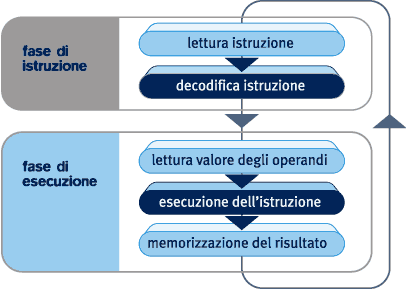
\includegraphics[width=.75\textwidth]{img/fasi_esecuzione.png}
		\caption{Ciclo di esecuzione delle istruzioni.}
	\end{figure}\newpage

	\subsubsection{Macchina astratta}

	\noindent
	L'implementazione di un linguaggio \textbf{significa} considerare una macchina astratta poiché lavorando ad alto livello, le istruzioni vengono interpretate e dunque si ignorano momentaneamente il linguaggio binario e la macchina fisica.
	\begin{boxdef}
		Dato un linguaggio $L$ di programmazione, la \textcolor{Red3}{\textbf{macchina astratta}} $M_{L}$ per $L$ è un insieme di strutture dati ed algoritmi che permettono di memorizzare ed eseguire i programmi scritti in $L$.
	\end{boxdef}
	
	\noindent
	La collezione di strutture dati ed algoritmi è necessario per:
	\begin{itemize}
		\item Acquisire la prossima istruzione
		
		\item Gestire le chiamate e i ritorni dai sottoprogrammi
		
		\item Acquisire gli operandi e memorizzare i risultati delle operazioni
		
		\item Mantenere le associazioni fra nomi e valori denotati
		
		\item Gestire dinamicamente la memoria
	\end{itemize}

	\noindent
	In altre parole, una \textbf{macchina astratta} è la combinazione di una memoria che immagazzina i programmi e di un interprete che esegue istruzioni dei programmi.
	\begin{figure}[!htp]
		\centering
		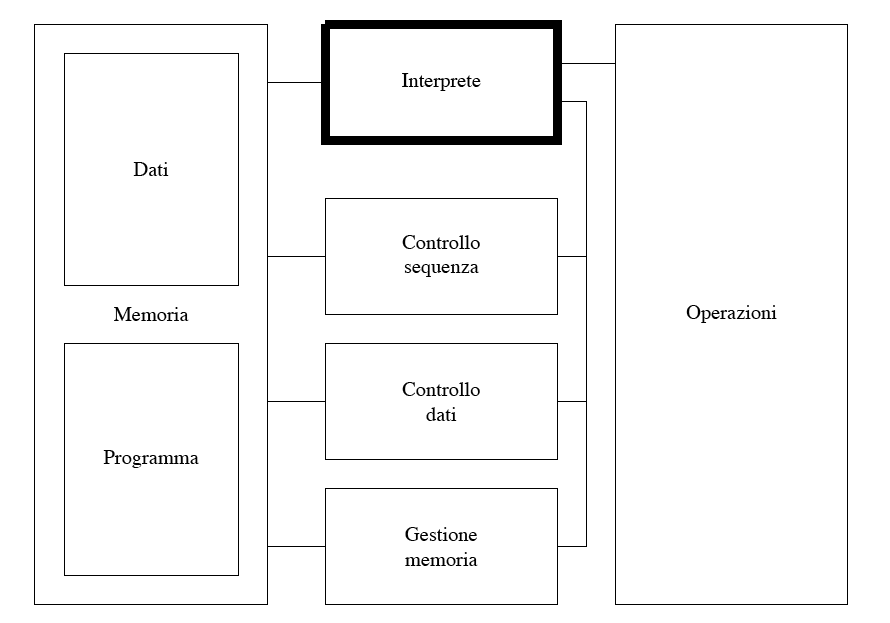
\includegraphics[width=\textwidth]{img/macchina_astratta.png}
		\caption{Rappresentazione di una macchina astratta.}
	\end{figure}
	
	\noindent
	Il \textbf{linguaggio} $L$ riconosciuto (interpretato) dalla macchina astratta $M_{L}$ viene chiamato \textbf{linguaggio macchina}. Formalmente, è l'insieme di tutte le stringhe interpretabili dalla macchina astratta $M$.\newpage
	
	\subsubsection{Realizzazione di una macchina astratta a vari livelli}
	
	Qualsiasi macchina astratta, per essere eseguita, deve prima o poi utilizzare qualche dispositivo hardware. Questo però non significa che tutte le macchine sono realizzate a livello hardware. Infatti, la realizzazione di una macchina astratta può avvenire tre categorie:
	\begin{itemize}
		\item \textcolor{Red3}{\textbf{Realizzazione hardware (HW)}}. Sempre possibile e concettualmente semplice. Il linguaggio macchina è il linguaggio fisico/binario e si realizza mediante dispositivi fisici. Data la sua lontananza dai linguaggi ad alto livello, la loro programmazione risulta complessa. Questo è uno dei tanti motivi per cui viene usata solo per sistemi dedicati.
		
		\item \textcolor{Red3}{\textbf{Realizzazione firmware (FW)}}. Le strutture dati e gli algoritmi vengono simulati nella macchina mediante microprogrammi. Il linguaggio macchina è a basso livello e consiste in microistruzioni che specificano le operazioni di trasferimento dati tra registri. Il vantaggio è dato dalla velocità e la flessibilità maggiore rispetto all'hardware.
		
		\item \textcolor{Red3}{\textbf{Realizzazione software (SW)}}. Le strutture dati e gli algoritmi vengono realizzati tramite un linguaggio implementato. In questo modo è possibile scrivere programmi che interpretano i costrutti del linguaggio macchina simulando le funzionalità della macchina. La velocità viene diminuita ma aumenta molto la flessibilità.
	\end{itemize}\newpage

	\subsubsection{Realizzazione software e livelli di astrazione}
	
	Con la realizzazione software, vengono utilizzati linguaggi di programmazione ad alto livello poiché essi implementano una struttura suddivisa a livelli di astrazione. Ogni livello coopera in modo sequenziale ma allo stesso tempo è indipendente.
	
	\begin{figure}[!htp]
		\centering
		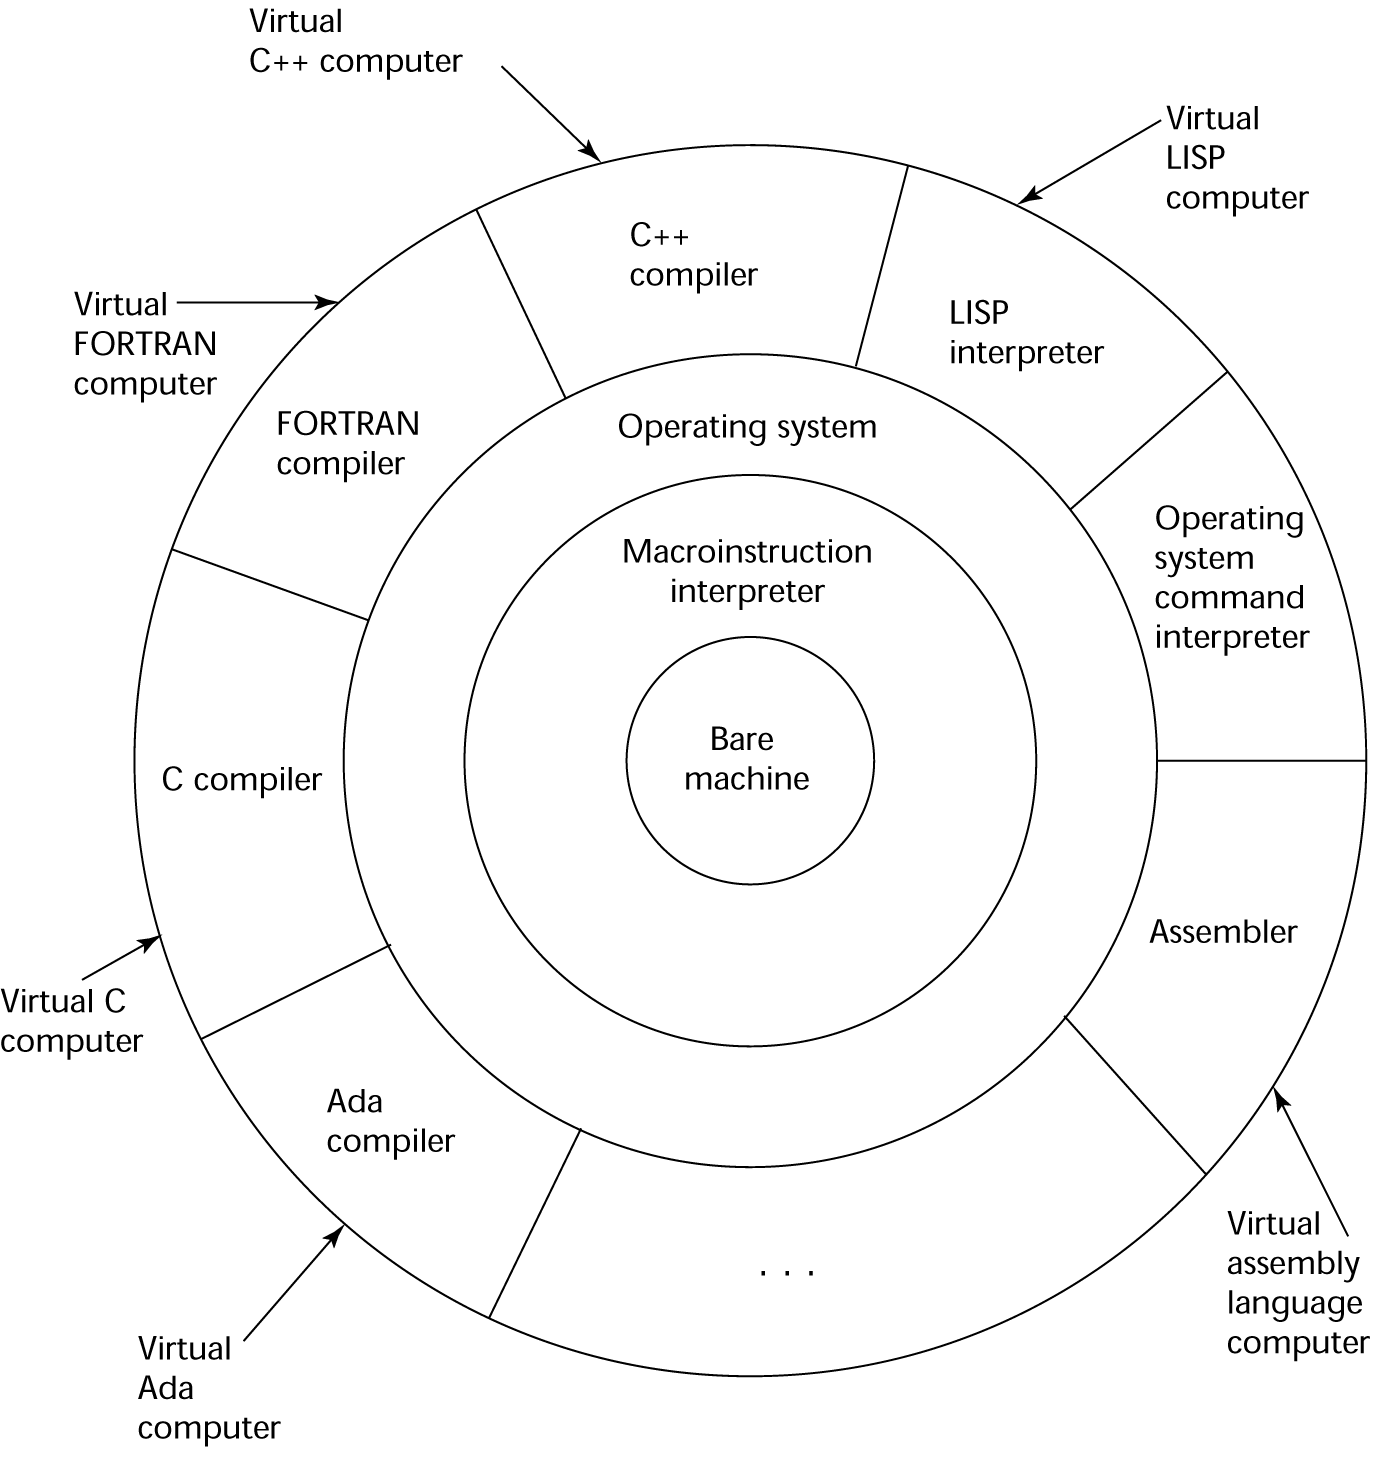
\includegraphics[width=.8\textwidth]{img/astrazione.png}
		\caption{Livelli di astrazione utilizzati dai linguaggi ad alto livello.}
	\end{figure}

	\noindent
	Quindi, la macchina può essere vista come una stratificazione di livelli di astrazione:
	\begin{figure}[!htp]
		\centering
		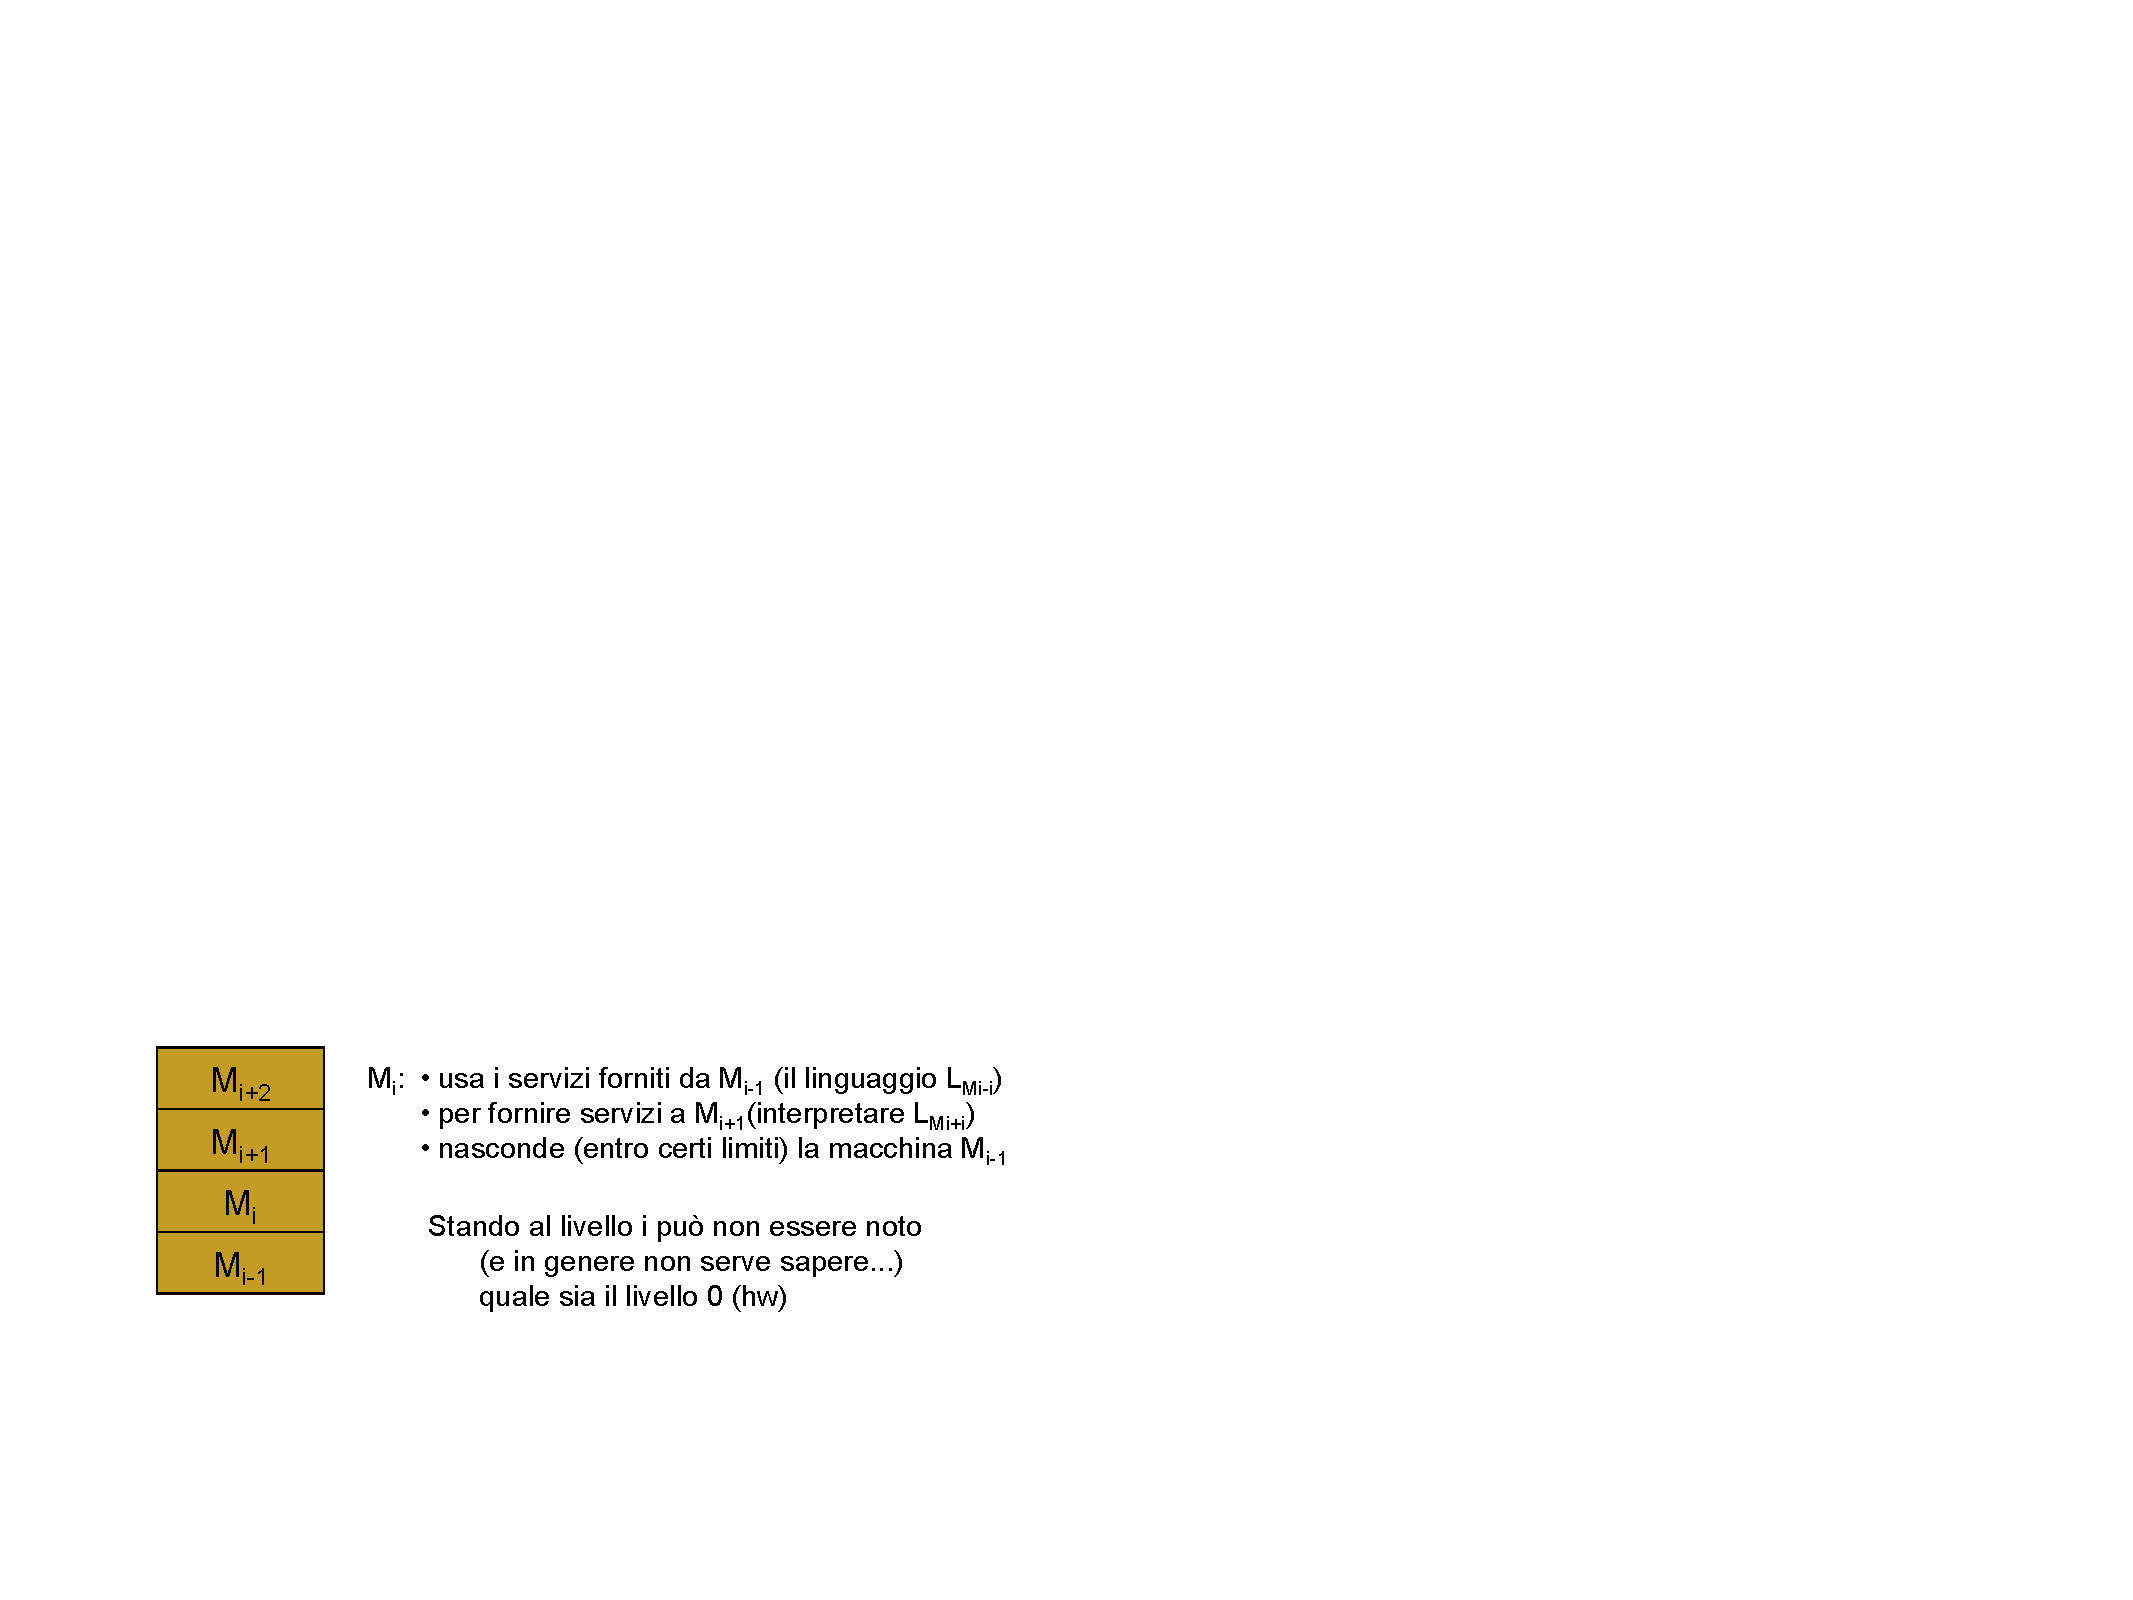
\includegraphics[width=.8\textwidth]{img/livelli_astrazione_macchina.pdf}
	\end{figure}\newpage

	\subsection{Realizzazione di una macchina a livello software/firmware}
	
	Sia $L$ un linguaggio da implementare e sia $M_{L_{0}}$ una macchina astratta a disposizione che ha come linguaggio macchina $L_{0}$. La macchina astratta $M_{L_{0}}$ è il livello su cui si vuole implementare il linguaggio $L$ e che mettette a disposizione di $M_{L}$ le sue funzionalità.\newline
	
	\noindent
	Dunque, la realizzazione di una macchina astratta $M_{L}$ consiste nel realizzare una macchina che \dquotes{traduce} il linguaggio $L$ (ad alto livello per esempio) in linguaggio macchina $L_{0}$, ovvero che interpreta tutte le istruzioni di $L$ come istruzioni di $L_{0}$. La traduzione avviene tramite due metodi a scelta:
	\begin{itemize}
		\item \textbf{Soluzione interpretativa}. Simulazione dei costrutti della macchina astratta $M_{L}$ da realizzare, mediante programmi scritti in $L_{0}$;
		\item \textbf{Soluzione compilativa}. Traduzione esplicita dei programmi di $L$ in corrispondenti programmi di $L_{0}$.
	\end{itemize}\newpage

	\subsubsection{Soluzione interpretativa: interprete}\label{interprete}
	
	La soluzione interpretativa prevede l'utilizzo di un interprete per la realizzazione di una macchina astratta. Un \textcolor{Red3}{\textbf{interprete}} è un programma $\mathrm{int}^{\mathrm{L_{0}, L}}$ che esegue, sulla macchina astratta per $L_{0}$, programmi $P^{L}$, scritti nel linguaggio di programmazione $L$, su un input fissato appartenente all'insieme di dati (input e output). In breve, un interprete è una \textbf{macchina universale} che preso un programma e un suo input, lo esegue su quell'input usando solo funzionalità messe a disposizione dal livello (macchina astratta) sottostante.
	\begin{boxdef}
		\begin{center}
			\textcolor{Red3}{\textbf{\emph{Notazioni}}}
		\end{center}
		\begin{itemize}
			\item $Prog^{L}$ è l'insieme di programmi scritti nel linguaggio di programmazione $L$;
			\item $D$ è l'insieme di dati, ovvero input e output;
			\item $P^{L}$ è il programma scritto nel linguaggio di programmazione $L$;
			\item Relazioni ovvie: $P^{L} \in Prog^{L}$ e $in, out \in D$;
			\item $\exec{P^{L}}: D \longrightarrow D$ è la notazione utilizzata per indicare che l'esecuzione del programma scritto nel linguaggio di programmazione $L$ con input $in$ è uguale all'output $out$. Quindi $\exec{P^{L}}\left(in\right) = out$.
		\end{itemize}
	\end{boxdef}
	\begin{boxdef}
		Un \textcolor{Red3}{\textbf{interprete formalmente}} è esprimibile nel seguente modo.\newline
		Si consideri un interprete da $L$ a $L_{0}$: dato $P^{L} \in Prog^{L}$ e $in \in D$, un interprete $int^{L, L_{0}}$ per $L$ su $L_{0}$ è un programma tale che:
		\begin{equation*}
			\exec{int^{L, L_{0}}}: \left(Prog^{L}\right) \longrightarrow D
		\end{equation*}
		e dunque:
		\begin{equation*}
			\exec{int^{L, L_{0}}}\left(P^{L}, in\right) = \exec{P^{L}}\left(in\right)
		\end{equation*}
	\end{boxdef}
	
	\noindent
	Anche un programma può essere utilizzato come dato di input in un altro programma. Si osservi il seguente diagramma:
	\begin{figure}[!htp]
		\centering
		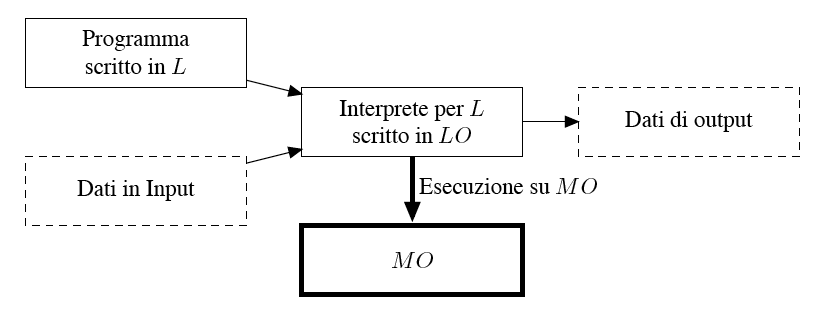
\includegraphics[width=\textwidth]{img/programma_input.png}
	\end{figure}
	
	\noindent
	Si noti come un programma scritto nel linguaggio $L$, insieme ad eventuali altri input, viene interpretato da un programma creato appositamente per eseguire questo compito su $L$, ma scritto in $L_{0}$. L'\textbf{esecuzione comporta una decodifica e non una traduzione esplicita}. Infatti, l'interprete simula ogni istruzione di $L$ utilizzando un certo insieme di istruzioni di $L_{0}$. Questa è la base dei linguaggi di scripting.
		
	\longline
	
	\subsubsection{Soluzione interpretativa: operazioni e struttura}
	
	Un interprete può eseguire una serie di \textbf{operazioni}:
	\begin{itemize}
		\item \textcolor{Red3}{\textbf{Elaborazione dei dati primitivi}}. I dati primitivi sono dati rappresentabili in modo diretto nella memoria, per esempio i numeri. Le elaborazioni di essi, sono implementate direttamente nella struttura della macchina;
		
		\item \textcolor{Red3}{\textbf{Controllo di sequenza delle esecuzioni}}. Non è altro che la gestione del flusso di esecuzione delle istruzioni, le quali non sempre sono sequenziali, tramite alcune strutture dati;
		
		\item \textcolor{Red3}{\textbf{Controllo dei dati}}. Recupero dei dati necessari per eseguire le istruzioni. I dati possono riguardare le modalità di indirizzamento della memoria e l'ordine con cui recuperare gli operandi;
		
		\item \textcolor{Red3}{\textbf{Controllo della memoria}}. È necessaria una gestione della memoria per allocare dati e programmi. Cambia a seconda del tipo di realizzazione della macchina astratta:
		\begin{itemize}
			\item Realizzazione hardware (HW): la gestione è semplice poiché nella peggiore delle ipotesi, i dati potrebbero essere rimasti sempre nelle stesse locazioni.
			
			\item Realizzazione software (SW): la gestione è complessa ed esistono costrutti di allocazione e deallocazione che richiedono alcune strutture dati (e.g. pile) e operazioni dinamiche.
		\end{itemize}
	\end{itemize}
	Date le operazioni elencate, il \textcolor{Red3}{\textbf{ciclo di esecuzione di un interprete}} è il seguente:
	\begin{lstlisting}[language=C]
begin
	go := true;
	while go do begin
		FETCH(OPCODE, OPINFO) at PC
		DECODE(OPCODE, OPINFO)
		if OPCODE needs ARGS then FETCH (ARGS)
		case OPCODE of
			OP1: EXECUTE(OP1, ARGS)
			...
			OPn: EXECUTE(OPn, ARGS)
			HLT: go := false;
		if OPCODE has result then STORE(RES);
		PC := PC + SIZE(OPCODE);
	end
end \end{lstlisting}
	\begin{itemize}
		\item Righe 1-3: finché \textsf{go} ha il valore \textsf{true}, il codice viene eseguito;
		\item Riga 4: estrazione dell'istruzione riferita ad \textsf{OPCODE} (controllo sequenza 1 su 2);
		\item Righe 5: decodifica dell'istruzione estratta alla riga precedente;
		\item Riga 6: prelievo dalla memoria gli operandi richiesti da \textsf{OPCODE} e nelle modalità individuate (controllo dati 1 su 2);
		\item Righe 7-11: esecuzione delle operazioni;
		\item Riga 12: se l'operazione ha un risultato da salvare, allora viene salvato in memoria (controllo dati 2 su 2);
		\item Riga 13: viene incrementato il \emph{program counter} (PC) per eseguire la prossima istruzione (controllo sequenza 2 su 2).
	\end{itemize}
	Il ciclo continua ad essere eseguito finché la variabile \textsf{go} ha valore \textsf{true}. Inoltre, le istruzioni riferite al program counter sono chiamate istruzioni di \textbf{controllo sequenza} (CS) perché manipolano e accedono al program counter. Mentre le operazioni di memorizzazione/estrazione sugli argomenti si chiamano \textbf{controllo dati} (CD).
	\begin{figure}[!htp]
		\centering
		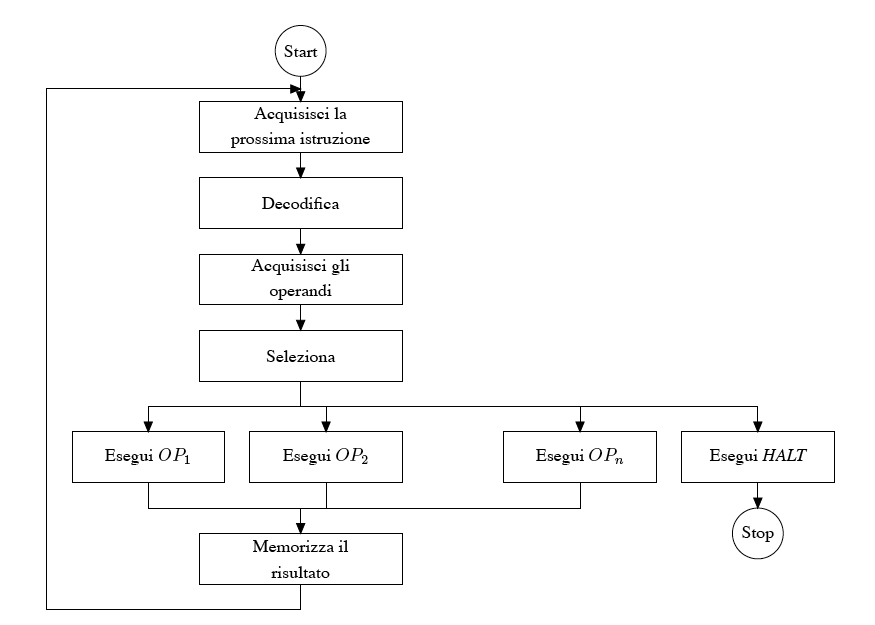
\includegraphics[width=\textwidth]{img/ciclo_esecuzione_interprete.png}
		\caption{Diagramma a blocchi della struttura di un interprete.}
	\end{figure}\newpage

	\subsubsection{Soluzione interpretativa: pro e contro}
	
	\begin{itemize}
		\item \textcolor{Green4}{\textbf{Pro:}}
		\begin{itemize}
			\item \textbf{Facilità di interazione \emph{run-time}}. Interpretazione al momento dell'esecuzione consente di interagire direttamente con l'esecuzione del programma (\emph{debugging});
			\item Velocità nello sviluppo applicativo di un interprete, quindi \textbf{tempi ridotti per la sua creazione};
			\item Utilizzo della \textbf{memoria ridotto} rispetto ad un compilatore.
		\end{itemize}

		\item \textcolor{Red3}{\textbf{Contro:}}
		\begin{itemize}
			\item Tempi di decodifica sommati a quelli d'esecuzione ogni volta che un'istruzione viene eseguita, si traduce in un'\textbf{esecuzione lenta} e quindi una scarsa efficienza della macchina.
		\end{itemize}
	\end{itemize}\newpage
	
	\subsubsection{Soluzione compilativa: compilatore}\label{compilatore}

	Un \textcolor{Red3}{\textbf{compilatore}} è un programma $\mathrm{comp}^{L_{0}, L}$ che \textbf{traduce}, preservando semantica e funzionalità, programmi scritti nel linguaggio di programmazione $L$ in programmi scritti in $L_{0}$, e quindi eseguibili direttamente sulla macchina astratta per $L_{0}$.
	Come l'interprete, anche il compilatore accetta un programma come input poiché viene considerato come dato.\newline
	
	\noindent
	\begin{boxdef}
		\begin{center}
			\textcolor{Red3}{\textbf{\emph{Notazioni}}}
		\end{center}
		\begin{itemize}
			\item $Prog^{L}$ è l'insieme di programmi scritti nel linguaggio di programmazione $L$;
			\item $D$ è l'insieme di dati, ovvero input e output;
			\item $P^{L}$ è il programma scritto nel linguaggio di programmazione $L$;
			\item Relazioni ovvie: $P^{L} \in Prog^{L}$ e $in, out \in D$;
			\item $\exec{P^{L}}: D \longrightarrow D$ rappresenta la semantica di $P^{L}$.
		\end{itemize}
	\end{boxdef}\:\newline

	\noindent
	\begin{boxdef}
		Un \textcolor{Red3}{\textbf{compilatore formalmente}} è esprimibile nel seguente modo.\newline
		Dato $P^{L} \in Prog^{L}$, un \textbf{compilatore} $\mathrm{comp}^{L, L_{0}}$ da $L$ a $L_{0}$ è un programma tale che:
		\begin{equation*}
			\exec{comp^{L, L_{0}}}: Progr^{L} \longrightarrow Progr^{L_{0}}
		\end{equation*}
		e dunque:
		\begin{equation*}
			\exec{comp^{L, L_{0}}}\left(P^{L}\right) = P^{L_{0}} \text{ tale che } \forall in \in D. \exec{P^{L_{0}}}\left(in\right) = \exec{P^{L}}\left(in\right)
		\end{equation*}
	\end{boxdef}\:\newline
	
	\noindent
	Ovvero che l'esecuzione della compilazione del linguaggio $L$ a $L_{0}$ con input il programma scritto in $L$, l'output sia uguale al programma scritto nel linguaggio $L_{0}$; tale che per ogni input appartenente all'insieme dei dati, l'esecuzione del programma scritto in $L_{0}$ con input $in$, sia uguale all'esecuzione del programma scritto in $L$ con input $in$.\newpage

	\noindent
	Con un compilatore, la \textbf{traduzione} è \textbf{esplicita} poiché il codice in $L$ viene prodotto come output e non eseguito. Quindi, per eseguire il programma $P^{L}$ con input $in$, è necessario prima eseguire $comp^{L, L_{0}}$ con $P^{L}$ come input.
	L'esecuzione avverrà sulla macchina astratta $M_{A}$ del linguaggio in cui è scritto il compilatore. Il risultato dunque è un altro programma (compilato) $P^{L_{0}}$, scritto in $L_{0}$. Solo a questo punto è possibile eseguire $P^{L_{0}}$ su $M_{L_{0}}$ con input $in$.
	Un \textbf{esempio} di linguaggio compilato è il C.
	\begin{figure}[!htp]
		\centering
		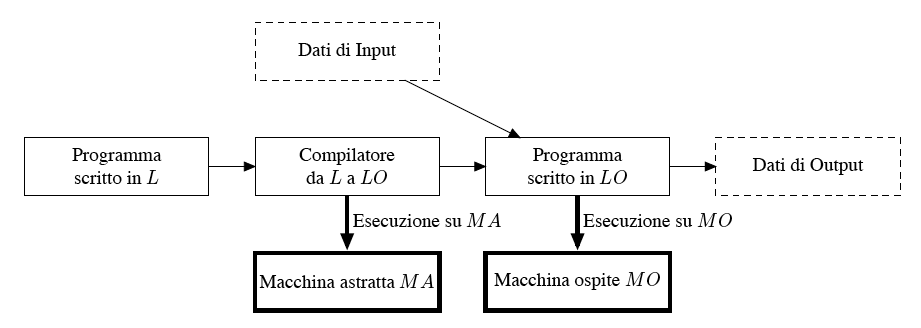
\includegraphics[width=\textwidth]{img/compilatore.png}
	\end{figure}\newpage

	\subsubsection{Soluzione compilativa: struttura}

	La compilazione deve tradurre un programma da un linguaggio ad un altro preservandone la semantica: si deve avere la certezza che il programma compilato faccia esattamente quello che faceva il sorgente. L'\textcolor{Red3}{\textbf{esecuzione}} di un compilatore si articola in varie fasi:
	\begin{figure}[!htp]
		\centering
		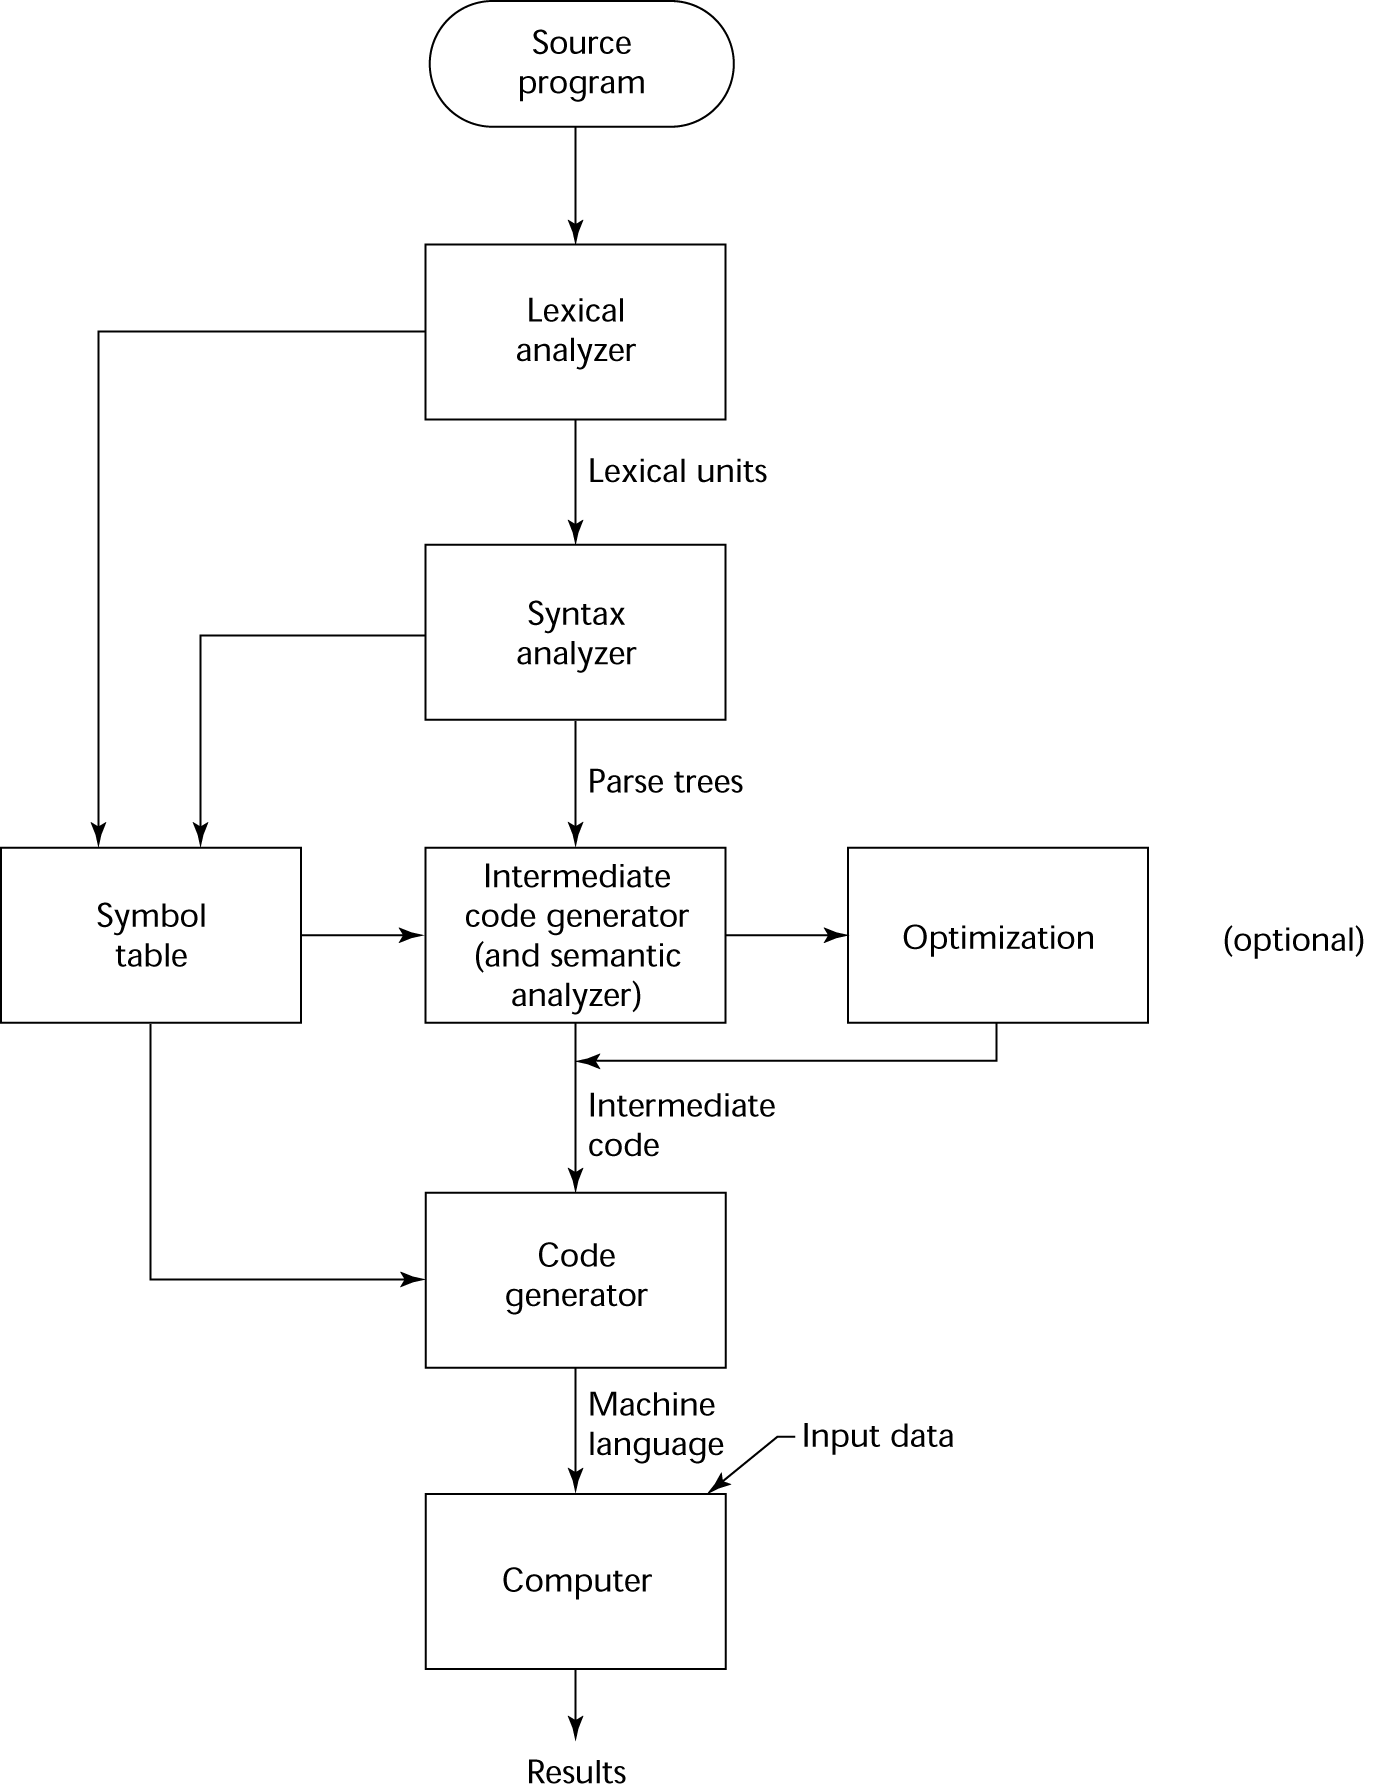
\includegraphics[width=.85\textwidth]{img/fasi_compilatore.png}
	\end{figure}
	
	\begin{itemize}
		\item \textcolor{Red3}{\textbf{Analisi lessicale}} (\emph{Lexical analyzer}), divide il programma in componenti sintattici primitivi chiamati \textbf{tokens} (identificatori, numeri, parole riservate). I \emph{tokens} sono coloro che formano i linguaggi regolari.\newline
		In altre parole, l'\textbf{analisi lessicale converte caratteri del programma sorgente in unità lessicali};\newpage

		\item \textcolor{Red3}{\textbf{Analisi sintattica}} (\emph{Syntax analyzer}), crea una rappresentazione ad albero della sintassi del programma. Ogni foglia è un \emph{token} e le foglie lette da sinistra verso destra costituiscono frasi ben formate del linguaggio. Inoltre, l'albero costituisce la struttura logica del programma e dunque nel momento in cui non fosse possibile costruire l'albero, significherebbe che qualche frase è illegale. Questo genere di evento si traduce in un errore di compilazione. Le frasi di token formano linguaggi CF.\newline
		In altre parole, l'\textbf{analisi sintattica trasforma unità lessicali in \emph{parse tree} che rappresentano la struttura sintattica del programma}.

		\item \textcolor{Red3}{\textbf{Tabella dei simboli}} (\emph{Symbol table}), memorizza le informazioni sui nomi presente nel programma, come gli identificatori, le chiamate di procedura, ecc.
		
		\item \textcolor{Red3}{\textbf{Analisi semantica}} (\emph{Semantic analyzer}), consente di rilevare errori semantici, grazie all'analisi semantica, e di generare codice intermedio che ha la caratteristica di essere indipendente dall'architettura (compito del \emph{Intermediate code generator}).

		\item \textcolor{Red3}{\textbf{Ottimizzazione}} (\emph{Optimization}), opzionale, consente di ottimizzare il codice.

		\item \textcolor{Red3}{\textbf{Generatore di codice}} (\emph{Code generator}), viene generato codice macchina che ha la caratteristica di essere dipendente dall'architettura.
	\end{itemize}

	\longline

	\subsubsection{Soluzione compilativa: pro e contro}
	
	\begin{itemize}
		\item \textcolor{Green4}{\textbf{Pro:}}
		\begin{itemize}
			\item \textbf{Esecuzione molto efficiente}, il codice viene anche ottimizzato;
		\end{itemize}

		\item \textcolor{Red3}{\textbf{Contro:}}
		\begin{itemize}
			\item \textbf{Interazione \emph{run-time} molto difficile};
			\item Un \textbf{errore} a \emph{run-time} è \textbf{difficile da associare} all'esatto comando del codice sorgente (debugging complesso);
		\end{itemize}
	\end{itemize}\newpage

	\subsubsection{Soluzione reale: ibrido}\label{ibrido}

	Nella realtà esiste un compromesso tra compilatore e interprete. Ovvero, una \textcolor{Red3}{\textbf{soluzione ibrida}} dove il linguaggio
	ad alto livello viene compilato in un linguaggio a più basso livello che poi viene interpretato.
	\begin{figure}[!htp]
		\centering
		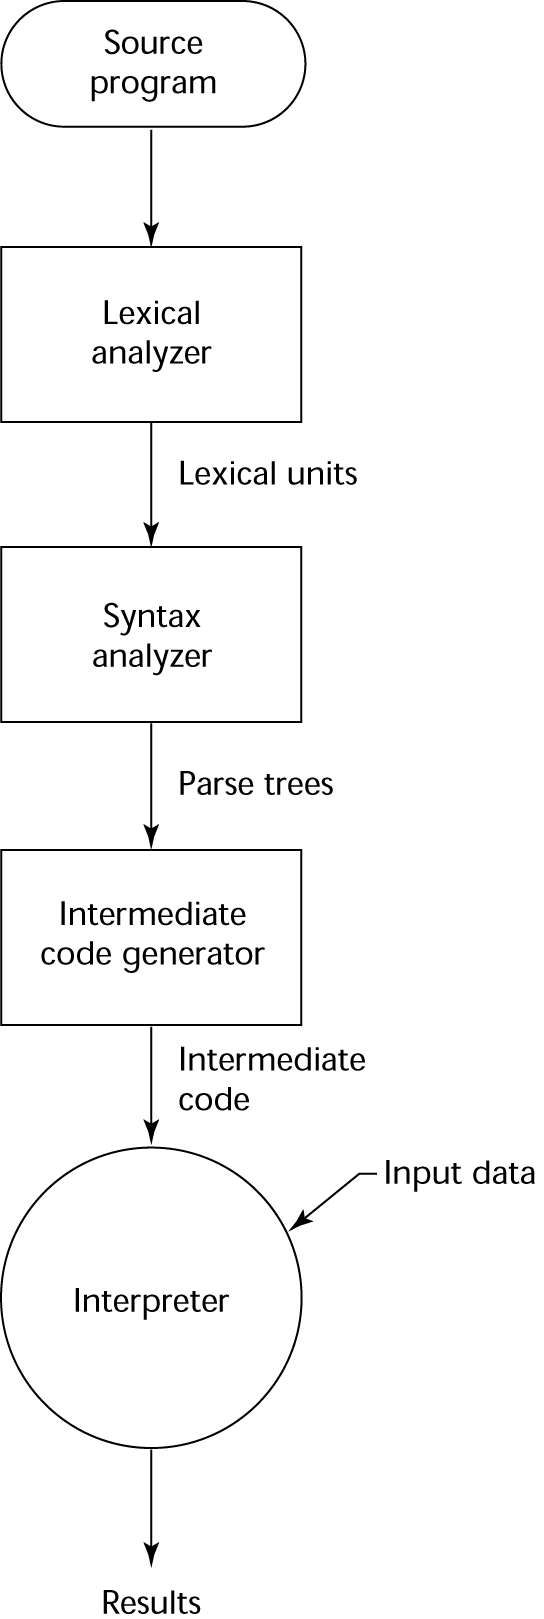
\includegraphics[width=.3\textwidth]{img/soluzione_reale_ibrida.png}
	\end{figure}

	\noindent
	Il \textbf{procedimento} è il seguente.\newline
	Si consideri il linguaggio ad alto livello $L$ per il quale si deve realizzare la macchina astratta $M_{L}$.\newline
	Il linguaggio $L$ viene quindi tradotto in un linguaggio intermedio $L_{Mi}$ la cui macchina astratta $M_{I}$ consiste in un interprete del linguaggio $L_{Mi}$ sulla macchina ospite $M_{O}$.\newline

	\noindent
	La separazione non è netta poiché vengono interpretati i costrutti lontani da $M_{O}$, mentre viene compilato il resto. Il passaggio chiave è la traduzione (compilazione) da $L$ ad un linguaggio intermedio (quello interpretato). Questo accade spesso nella realtà, specialmente con le \emph{system call} del sistema operativo. In parole povere, si cerca di trovare una connessione a metà strada.\newpage
	\begin{figure}[!htp]
		\centering
		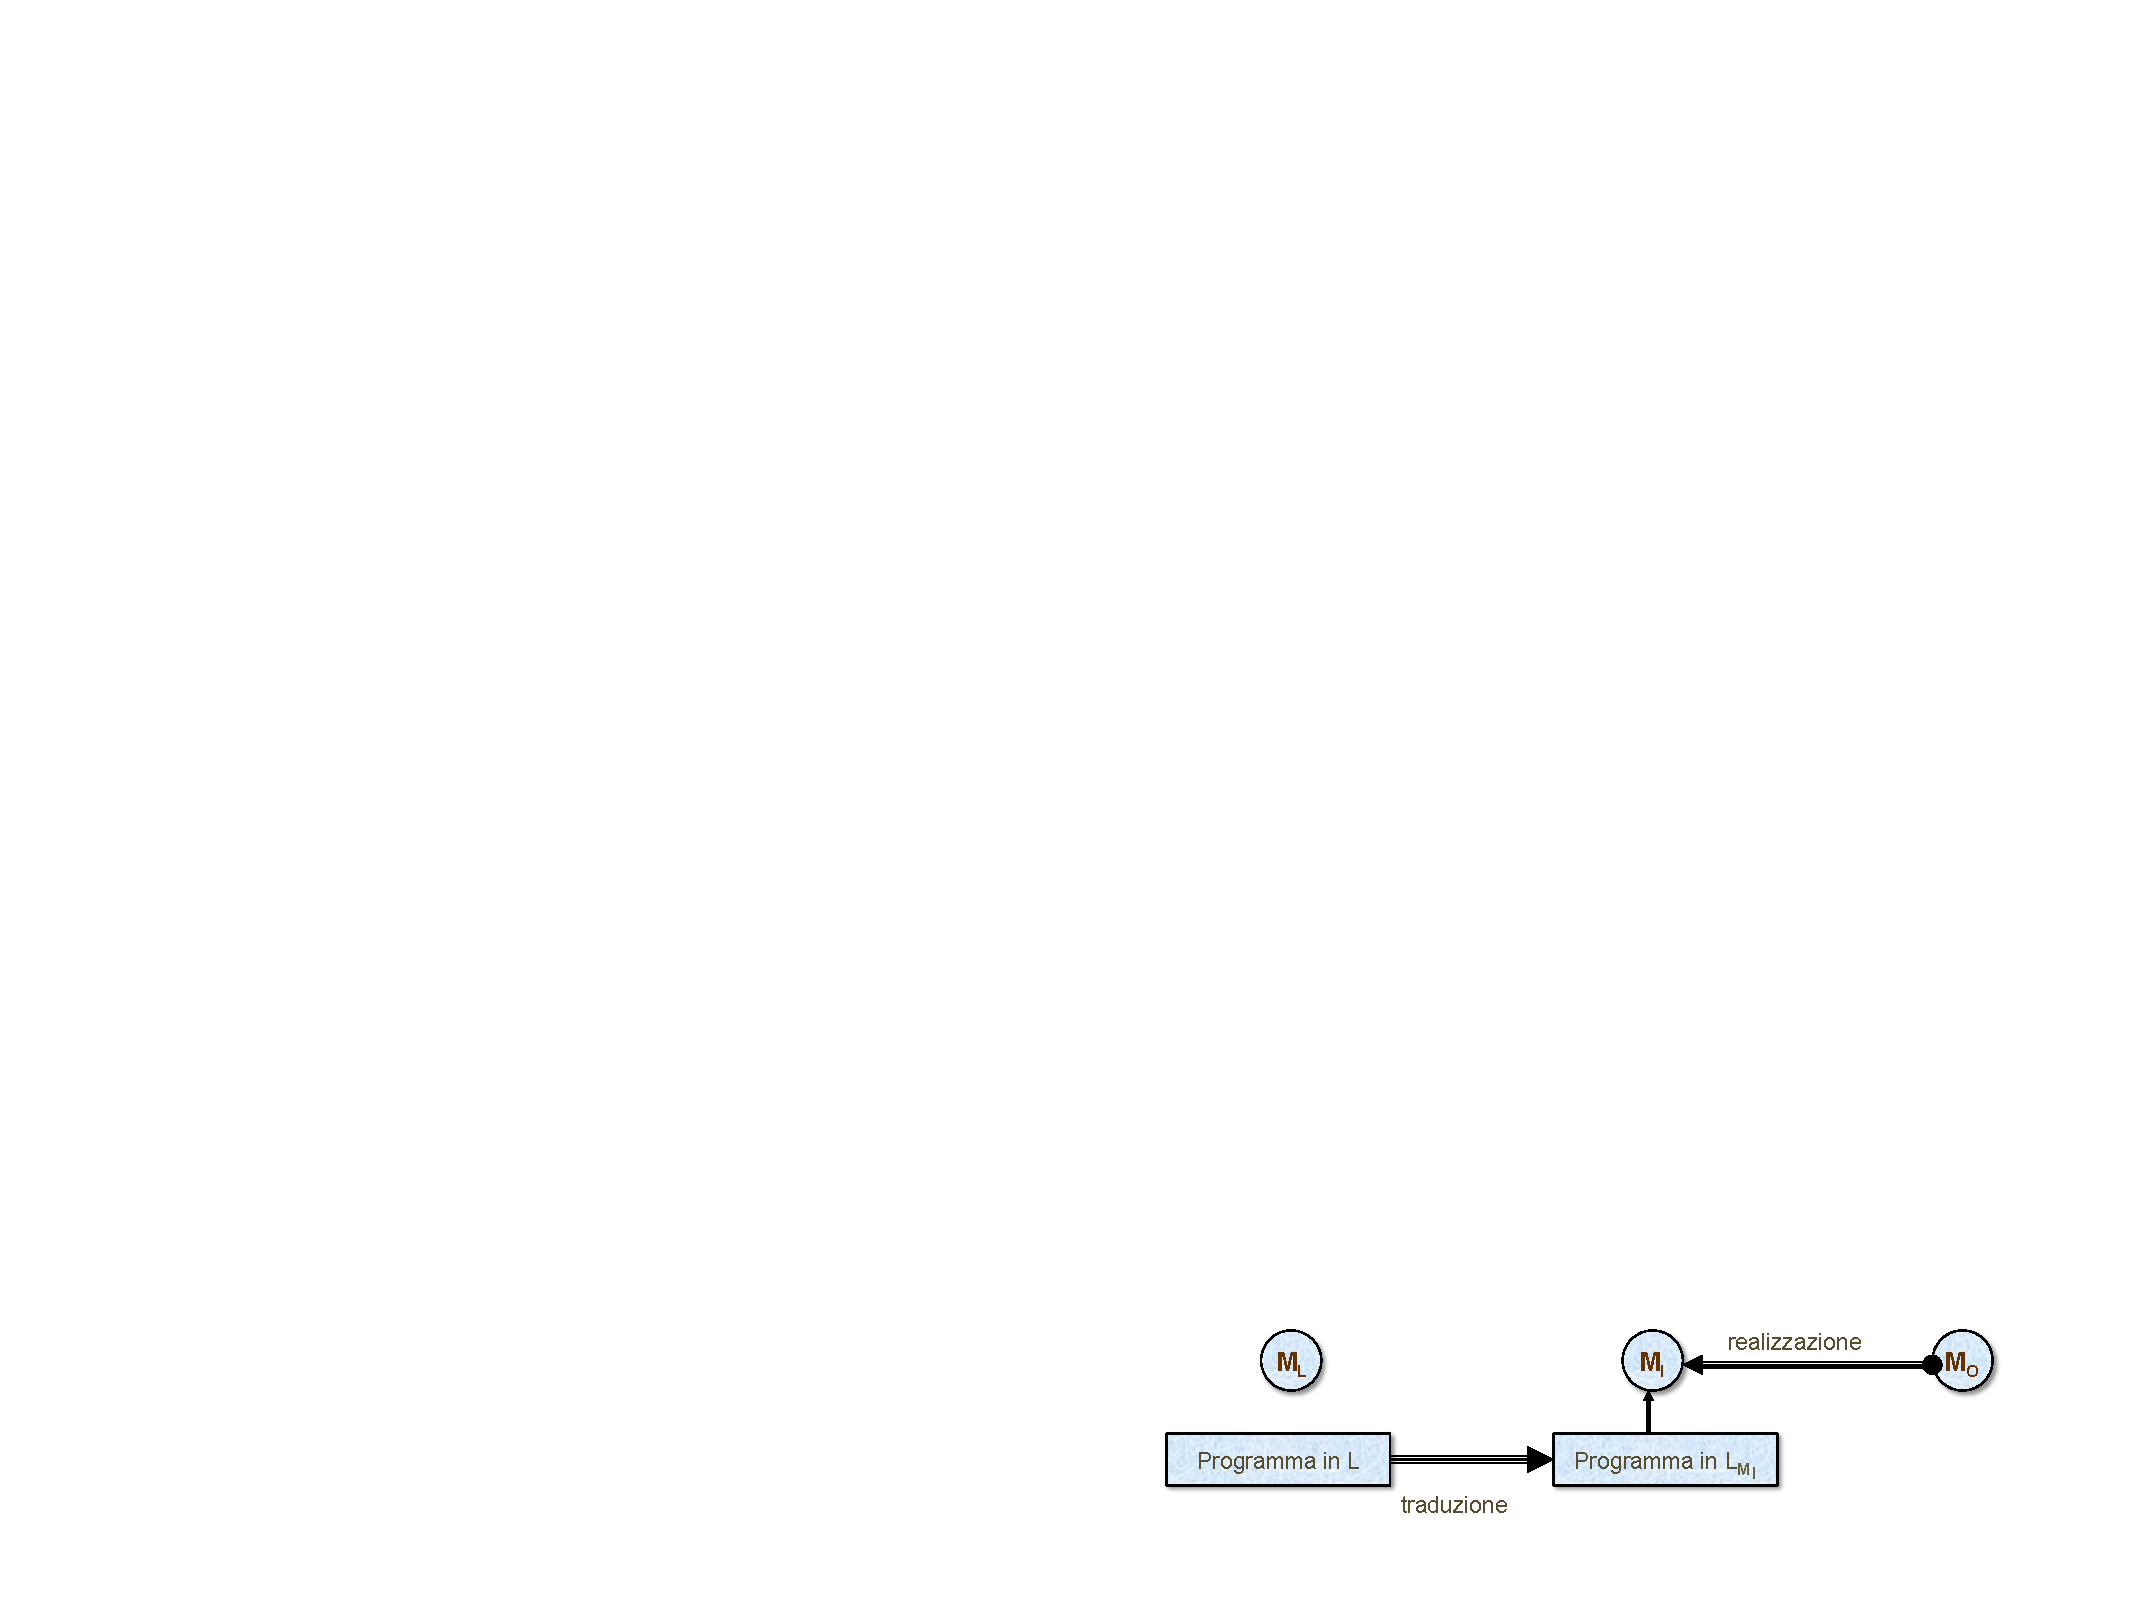
\includegraphics[width=\textwidth]{img/soluzione_ibrida_system_call.pdf}
		\caption{Soluzione ibrida con le \emph{system call}.}
	\end{figure}

	\longline

	\subsection{Sintesi}

	Nell'evoluzione dei linguaggi di programmazione, esistono fondamentalmente tre situazioni possibili:
	\begin{itemize}
		\item \textcolor{Red3}{\textbf{Interprete puro}} (paragrafo \ref{interprete}), $M_{L} = M_{I}$ (interprete per $L$ realizzato sulla macchina ospite $M_{O}$). Per esempio i linguaggi logici e funzionali, e di scripting (JS, PHP, ...)

		\item \textcolor{Red3}{\textbf{Compilatore}} (paragrafo \ref{compilatore}), macchina intermedia $M_{I}$ realizzata per estensione sulla macchina ospite $M_{O}$. Per esempio i linguaggi imperativi come C, C++, Pascal
		
		\item \textcolor{Red3}{\textbf{Implementazione mista}} (paragrafo \ref{ibrido}), traduzione dei programmi da $L$ ad un linguaggio intermedio $L_{Mi}$. I programmi $L_{Mi}$ sono poi interpretati sulla macchina ospite $M_{O}$. Per esempio, Java con il suo linguaggio intermedio Java bytecode, Pascal con il suo linguaggio intermedio P-code.
	\end{itemize}\newpage

	\section{Descrivere i linguaggi}

	Un \textbf{linguaggio di programmazione} è un linguaggio naturale, ma con alcune semplificazioni e \textbf{non ambiguo}. Quindi, per descriverli è necessario affrontare alcune tematiche:
	\begin{itemize}
		\item Grammatica, o meglio la \textcolor{Red3}{\textbf{sintassi}}: costituisce l'\textbf{insieme delle regole che consentono di costruire frasi corrette}. Viene quindi individuato l'alfabeto con cui sono costruite le frasi, le parole che compongono le frasi e infine viene eseguito un controllo della grammatica per verificare se le frasi le rispettano (il compito di verificare è assegnato al \textbf{\emph{parsing}});
		\item \textcolor{Red3}{\textbf{Semantica}}: nei linguaggi rappresenta la \textbf{relazione tra segni} (frasi legali) \textbf{e significati} (entità autonome che esistono indipendentemente dai segni utilizzati). Per esempio, la semantica di un programma può essere la funzione matematica calcolata dal programma. Solitamente la semantica viene specificata descrivendo gli effetti della sintassi su una rappresentazione astratta della macchina, chiamata \textbf{stato};
		\item \textcolor{Red3}{\textbf{Pragmatica}}: analisi delle \textbf{frasi che hanno lo stesso significato, ma possono essere utilizzate diversamente} in modo dipendente dal contesto linguistico;
		\item \textcolor{Red3}{\textbf{Implementazione}}: aspetti riguardanti la tecnica di implementazione utilizzata, i vincoli dell'architettura o della macchina, l'interfaccia del sistema operativo, gestione degli errori.\newline
		In sintesi, sono tutti gli aspetti che hanno effetto sul funzionamento del linguaggio ma che dipendono dalla macchina su cui esso viene eseguito.
	\end{itemize}\newpage

	\subsection{Sintassi}

	\subsubsection{Definizione e notazione}

	Le regole sintattiche (\textcolor{Red3}{\textbf{sintassi}}) del linguaggio specificano quali stringhe di caratteri sono legali nel linguaggio.\newline
	
	\noindent
	La terminologia linguistica utilizzata è la seguente:
	\begin{itemize}
		\item Una \textbf{parola} è una stringa di caratteri su un alfabeto;
		\item Una \textbf{frase} è una sequenza, ben formata, di parole;
		\item Una \textbf{linguaggio} è un insieme di frasi.
	\end{itemize}
	Invece, la \textbf{terminologia tecnica} utilizzata nel mondo dell'informatica è la seguente:
	\begin{itemize}
		\item Le \textbf{parole} vengono chiamate \textcolor{Red3}{\textbf{lessemi}}. Un lessema è una \textbf{parola con un significato specifico}, nella grammatica corrisponde ad un terminale. Rappresenta anche l'\textbf{unità minima sintattica}, ovvero quella a più basso livello di un linguaggio di programmazione (e.g. \textsf{begin}). \textbf{Per esempio}, in $index = 2$, sia $index$, $=$, che $2$ sono lessemi;
		\item Le \textbf{frasi} vengono chiamate \textcolor{Red3}{\textbf{\emph{token}}}. Essi corrispondono agli elementi delle categorie sintattiche del linguaggio di programmazione, e nella grammatica corrispondono alle sequenze generate dai simboli non terminali. \textbf{Per esempio}, con $index = 2$, il token è l'intera definizione;
		\item Il \textcolor{Red3}{\textbf{programma}} è una sequenza/composizione sequenziale, nella grammatica, di frasi ben formate;
		\item I linguaggi diventa il \textcolor{Red3}{\textbf{linguaggio di programmazione}}, ovvero tutti gli strumenti formali che lo definiscono.
	\end{itemize}\newpage

	\subsubsection{Descrivere la sintassi}

	Nei linguaggi di programmazione, il \textbf{linguaggio dei lessemi} è in generale sempre un linguaggio \textbf{regolare}, ovvero \textbf{riconosciuto} da un automa a stati finiti.
	\begin{boxdef}
		Si definisce \textcolor{Red3}{\textbf{riconoscitore}}, uno \textbf{strumento di riconoscimento che legge in input stringhe sull'alfabeto del linguaggio e decide se la stringa appartiene o meno al linguaggio}.
	\end{boxdef}
	
	\noindent
	Per esempio, l'analisi sintattica, la quale riconosce lessemi, di un compilatore.\newline

	\noindent
	Sia $L$ un linguaggio su un alfabeto $\Sigma$, per \textbf{costruire un riconoscitore} è necessario avere un meccanismo $R$ in grado di leggere (input) le stringhe di caratteri e dire (output) se essa appartiene oppure no al linguaggio $L$. Si ricorda, che questo è possibile perché il linguaggio è regolare.\newline

	\noindent
	Il \textbf{linguaggio dei \emph{token}}, e quindi dei programmi, è in generale un \textbf{linguaggio \emph{context-free} (CF)}, quindi viene \textbf{generato} da una grammatica CF.
	\begin{boxdef}
		Si definisce \textcolor{Red3}{\textbf{generatore}}, uno \textbf{strumento che genera stringhe di un linguaggio}. Inoltre, un generatore può determinare se la sintassi di una particolare chiave è sintatticamente corretta confrontandola con la struttura del generatore (\emph{parser}).
	\end{boxdef}\newpage

	\subsection{Grammatiche \emph{context-free}}

	Una \textcolor{Red3}{\textbf{grammatica libera dal contesto}} (o \emph{context-free}, CF) è una quadrupla $G = \left\langle V, T, P, S \right\rangle$, dove:
	\begin{itemize}
		\item $V$ è un insieme finito di variabili, chiamati anche simboli non terminali. Rappresenta le \textbf{categorie sintattiche}, ovvero gli \textbf{elementi della frase};
		\item $T$ è un insieme finito di simboli terminali $\left(V \cap T = \emptyset\right)$. Rappresenta il \textbf{vocabolario}, ovvero la \textbf{collezione di lessemi};
		\item $P$ è un insieme finito di produzioni; ogni produzione è della forma $A \rightarrow \alpha$, dove:
		\begin{itemize}
			\item $A \in V$ è una variabile
			\item $\alpha \in \left(V \cup T\right)$
		\end{itemize}
		Questo insieme rappresenta la \textbf{collezione di regole di formazione/composizione};
		\item $S \in V$ è una variabile speciale, chiamata simbolo iniziale. Rappresenta la \textbf{categoria delle frasi}.
	\end{itemize}
	La proprietà CF è anche uno svantaggio per i linguaggi di programmazione, infatti tali grammatiche non riescono a catturare vincoli contestuali. Per esempio, poter utilizzare una variabile se e solo se questa è stata precedentemente dichiarata/definita.\newpage

	\subsection{Notazione BNF}

	La \textcolor{Red3}{\textbf{BNF}} è un metalinguaggio, ovvero un \textbf{linguaggio usato per descrivere altri linguaggi}. Venne introdotto perché in passato accadeva che chi progettava ogni implementazione di un compilatore, dava significati diversi agli stessi costrutti. Questo si traduceva che programmi scritti in un linguaggio di programmazione, sviluppati per macchine diverse, non erano confrontabili.\newline

	\noindent
	Questa notazione è utilizzata per descrivere grammatiche CF, dove si usano intere parole come simboli terminali, i non terminali sono identificati racchiudendoli tra parentesi angolate $<>$, e per le produzioni si utilizza il simbolo $\Coloneqq$ al posto della freccia.
	\begin{equation*}
		\begin{array}{lll}
			<A> & \Coloneqq & \alpha <B> \gamma \hspace{1em} | \hspace{1em} \alpha \\
			\\
			<B> & \Coloneqq & \varepsilon \hspace{1em} | \hspace{1em} \beta_{1} \hspace{1em} | \hspace{1em} \beta_{2}
		\end{array}
	\end{equation*}
	Il suo significato è esattamente identico a quello delle grammatiche. Quindi:
	\begin{itemize}
		\item \textbf{Non terminali} sono astrazioni utilizzate per rappresentare classi di strutture sintattiche;
		\item \textbf{Terminali} sono lessemi;
		\item Ogni regola ha una parte \textbf{sinistra} contenente un \textbf{non terminale};
		\item Ogni regola ha una parte \textbf{destra} contenente una \textbf{stringa di terminali e non terminali}.
	\end{itemize}
	Esiste anche la \textcolor{Red3}{\textbf{variante EBNF}} che aggiunge la possibilità di rappresentare le \textbf{opzioni}:
	\begin{itemize}
		\item Le \textbf{parentesi quadre} $[\:]$ indicano nessuna o un'occorrenza del contenuto;
		\item Le \textbf{parentesi graffe} $\{\:\}$ indicano nessuna o più occorrenze di quanto contenuto.
		\item La \textbf{virgola} $,$ consente di esprimere più opzioni in or logico.
	\end{itemize}
	Un esempio:
	\begin{equation*}
		<A> \Coloneqq \alpha \: \left[\beta_{1}, \beta_{2}\right] \: \gamma \hspace{1em} | \hspace{1em} \alpha \: \gamma \hspace{1em} | \hspace{1em} \gamma
	\end{equation*}\newpage

	\subsection{Descrivere un semplice linguaggio imperativo}

	Un \textbf{linguaggio può essere descritto in modo informale} descrivendo quali caratteristiche inserire e il loro significato:
	\begin{itemize}
		\item Niente dichiarazioni;
		\item Solo variabili ed espressioni booleane;
		\item Assegnamento e composizione sequenziale;
		\item Comando condizionale;
		\item Comando iterativo (\emph{loop}).
	\end{itemize}
	Nonostante possa essere sufficiente per scrivere un programma corretto e interpretabile da un altro programmatore, esso \underline{non} è adeguato per costruire un compilatore o un interprete.\newline
	
	\noindent
	Per costruire un compilatore o un interprete è necessario scendere ad un livello più formale.\newline

	\noindent
	\textbf{È necessario che un linguaggio sia descritto a più livelli di astrazione ed ogni strato sia descritto da una grammatica}.

	\begin{figure}[!htp]
		\centering
		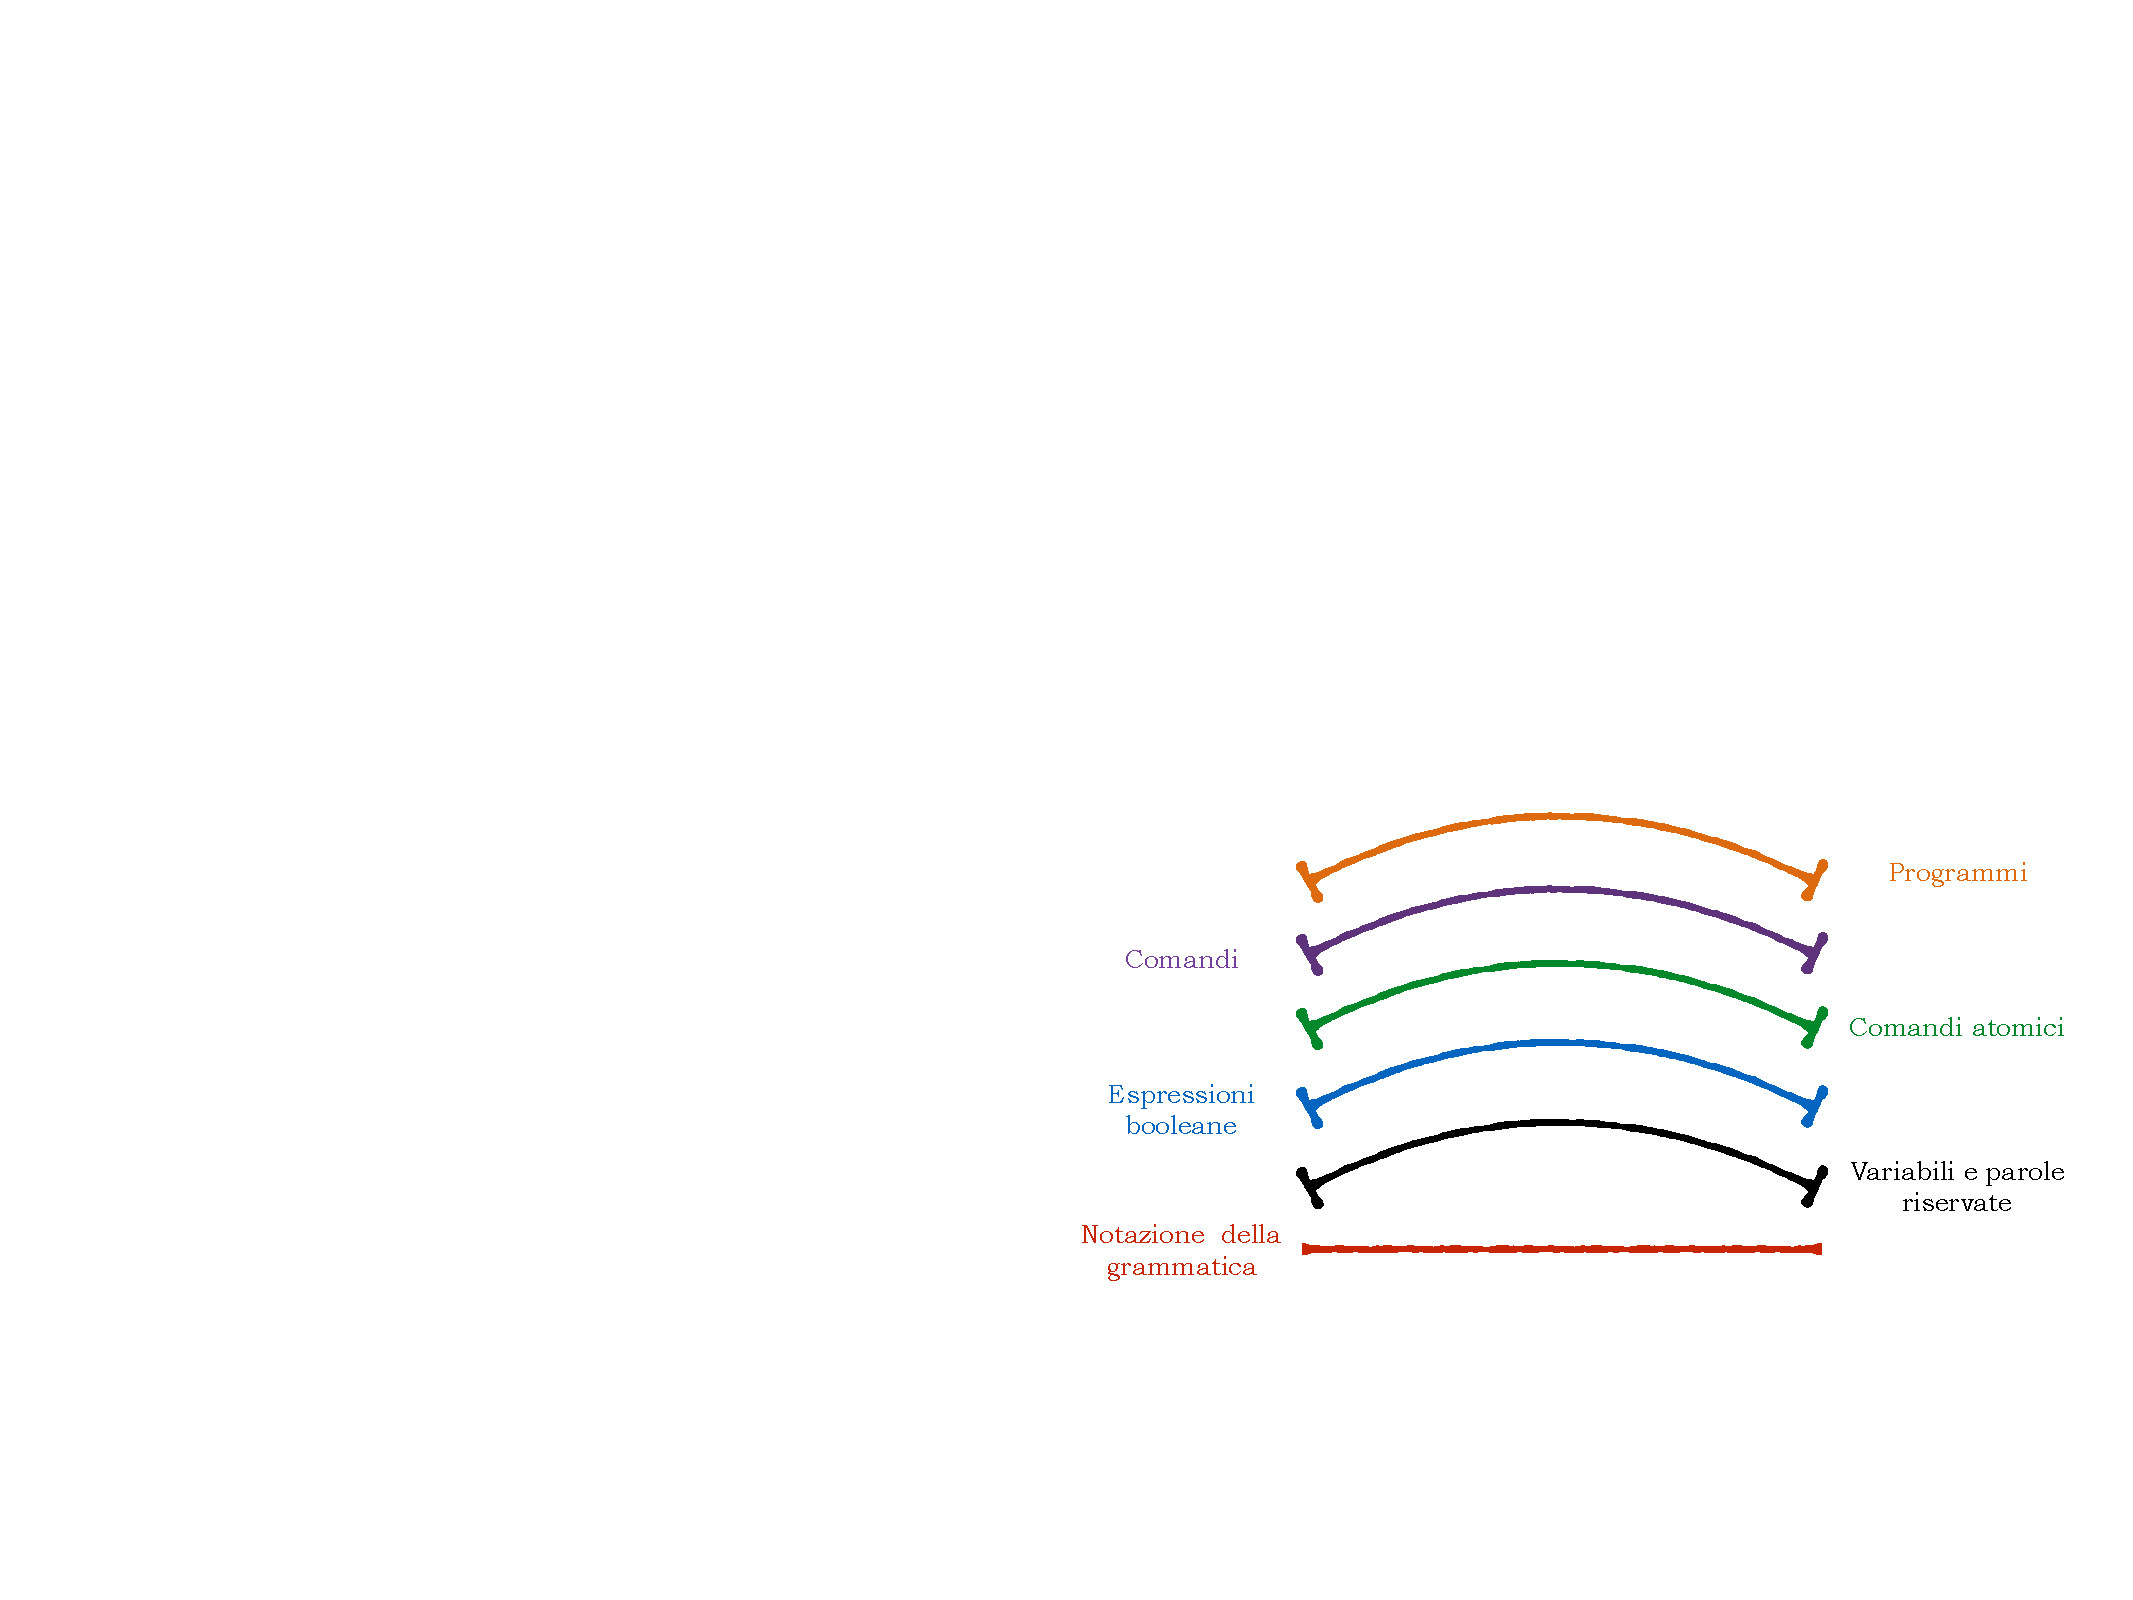
\includegraphics[width=\textwidth]{img/astrazione_linguaggi.pdf}
		\caption{Linguaggio descritto a più livelli di astrazione.}
	\end{figure}

	\noindent
	Un esempio di descrizione a più livelli:
	\begin{equation*}
		\begin{array}{lllll}
			\mathrm{<program>} 		&& S & \Coloneqq & C \\
			\\
			\mathrm{<com>}			&& C & \Coloneqq & A \hspace{1em} | \hspace{1em} C ; C \hspace{1em} | \hspace{1em} \mathrm{if} \: B \: \mathrm{then} \: C \: \mathrm{else} \: C \hspace{1em} | \hspace{1em} \mathrm{while} \: B \: \mathrm{do} \: C \\
			\\
			\mathrm{<atomic \: com>}&& A & \Coloneqq & v \Coloneq B \\
			\\
			\mathrm{<b-expr>}		&& B & \Coloneqq & \mathrm{true} \hspace{1em} | \hspace{1em} \mathrm{false} \hspace{1em} | \hspace{1em} v \hspace{1em} | \hspace{1em} \left(\mathrm{not} \: B\right) \hspace{1em} | \hspace{1em} \left(B \: \mathrm{and} \: B\right) \hspace{1em} | \hspace{1em} \left(B \: \mathrm{or} \: B\right)
		\end{array}
	\end{equation*}\newpage

	\subsection{Analisi semantica}

	Esistono dei vincoli che dipendono dal contesto. Per esempio, l'espressione:
	\begin{equation*}
		I \Coloneq R + 3
	\end{equation*}
	Potrebbe essere sintatticamente corretta ma illegale nel contesto in cui si trova. Infatti, se il linguaggio fosse fortemente \emph{tipato} e prima non ci fosse una dichiarazione di $R$ e di $I$, il comando sarebbe illegale.\newline

	\noindent
	Quindi, stringhe sintatticamente corrette per una certa grammatica sono legali sono in determinati contesti. Questo \textbf{vincolo sintattico} non può essere descritto mediante le grammatiche CF.\newline

	\noindent
	Esistono due \textbf{soluzioni}:
	\begin{itemize}
		\item Utilizzare grammatiche contestuali (CSG). Tuttavia, non esistono algoritmi lineari per il riconoscimento di stringhe generate, quindi non esistono algoritmi efficienti per effettuare il parser delle stringhe di una CSG.
		\item Utilizzare controlli \emph{ad hoc}.
	\end{itemize}
	A causa dei problemi con le grammatiche contestuali, la scelta ricade nell'utilizzare una specifica del linguaggio mediante una grammatica CF (\textbf{sintassi}) e successivamente, come parte della semantica (\textcolor{Red3}{\textbf{semantica statica}}) specificare i vincoli contestuali.\newpage

	\subsection{Semantica dinamica}

	La \textbf{semantica} ricerca esattezza e flessibilità:
	\begin{itemize}
		\item \textbf{Esattezza}: descrizione precisa e non ambigua di ogni costrutto sintatticamente corretto, per sapere cosa accadrà durante l'esecuzione
		\item \textbf{Flessibilità}: nessuna anticipazione delle scelte che devono essere demandate dall'implementazione.
	\end{itemize}
	La \textcolor{Red3}{\textbf{semantica dinamica}} risponde ad alcune problematiche, come il significato di alcuni comandi, che cosa fanno i costrutti, generatori di compilatori. Il suo \textbf{utilizzo è fondamentale poiché specifica gli effetti della sintassi sulla rappresentazione astratta della macchina}, quest'ultima chiamata \textbf{stato}.\newline
	Quindi, per ogni costrutto, va descritto il significato della sua esecuzione come trasformazione di stato. Infatti, l'astrazione della macchina nel concetto di stato consente di dare al costrutto un significato puro, indipendente dalla macchina, quindi senza restrizioni.\newline

	\noindent
	\begin{boxdef}
		La \textcolor{Red3}{\textbf{semantica}} \textbf{attribuisce un significato ad ogni frase sintatticamente corretta}.
	\end{boxdef}
	\begin{boxdef}
		Con \textcolor{Red3}{\textbf{significato}} \textbf{si intendono le entità autonome che esistono indipendentemente dai segni che vengono utilizzati per descriverle}.
	\end{boxdef}

	\noindent
	Esiste un \textbf{legame forte tra sintassi e semantica}:
	\begin{itemize}
		\item La \textbf{sintassi} è utilizzato come metodo finito per rappresentare un insieme infinito di programmi, la cui sola cosa analizzabile è la struttura;
		\item La \textbf{semantica} è utilizzata come metodo finito, infatti segue la struttura della sintassi, per dare significato a tutti gli elementi dell'insieme infinito dei programmi.
	\end{itemize}\newpage

	\subsection{Induzione matematica e strutturale}

	La semantica segue la struttura della sintassi, mentre quest'ultima è definita descrivendo gli elementi base e componendo questi elementi, attraverso regole, in elementi composti.\newline
	
	\begin{boxdef}
		Questa forma di definizione si chiama \textcolor{Red3}{\textbf{induzione}} e più formalmente è: data un insieme $A$ ed una relazione binaria $< \subseteq A \times A$ ben fondata (senza catene discendenti infinite), se $A = Nat$ si ha \textbf{induzione matematica}; se $A = L\left(G\right)$ è un linguaggio generato da una grammatica $G$, allora si ha \textbf{induzione strutturale}.
	\end{boxdef}\:\newline

	\noindent
	\begin{boxdef}
		Il \textcolor{Red3}{\textbf{principio di induzione strutturale}} si basa sulla seguente definizione. Per dimostrare che una proprietà è valida per tutti gli elementi di una categoria sintattica:
		\begin{enumerate}
			\item \textbf{Base induttiva}: si dimostra la proprietà per tutti gli elementi base della categoria, quelli che non hanno nessun elemento come componente;
			\item \textbf{Passo induttivo}: si dimostra la proprietà per tutti gli elementi composti assumendo che la proprietà sia verificata da tutti i loro componenti immediati.
		\end{enumerate}
	\end{boxdef}\newpage

	\noindent
	Ecco una dimostrazione d'\textcolor{Green4}{\textbf{esempio}} di induzione.
	\begin{proof}[\textbf{Dimostrazione induttiva}]
		Dimostrare che:
		\begin{equation*}
			\sum_{i = 1}^{n} i = \dfrac{n \left( n + 1 \right)}{2} \hspace{2em} \text{con } n \ge 1
		\end{equation*}
		La \textbf{base induttiva} è con $n$ pari ad $1$, quindi sostituendo:
		\begin{equation*}
			n = 1 \hspace{2em} \sum_{i = 1}^{1} i = 1 = \dfrac{1 \left( 1 + 1 \right)}{2}
		\end{equation*}
		Per il \textbf{passo induttivo} si suppone che sia vero per $n$ considerando dunque come passo induttivo l'equazione iniziale. Si dimostra per $n + 1$:
		\begin{equation*}
			\begin{array}{rll}
				\displaystyle\sum_{i=1}^{n+1} i & = & \dfrac{ \left(n+1\right) \left(n+2\right) }{2} \\
				\\
				\displaystyle\sum_{i=1}^{n+1} i \triangleq \underbrace{\sum_{i=1}^{n} i + \left(n+1\right)}_{\text{per definizione}} & = & \underbrace{\dfrac{n \left(n+1\right)}{2}}_{\text{ip. induttiva}} + \: n + 1 \\
				\\
				& = & \dfrac{n \left(n+1\right) + 2n + 2}{2} = \dfrac{n^{2} + n + 2n + 2}{2} \\
				\\
				& = & \dfrac{\left(n+1\right) n + \left(n+1\right) 2}{2} = \dfrac{\left(n+1\right) \left(n+2\right)}{2}
			\end{array}
		\end{equation*}
	\end{proof}\newpage

	\subsection{Un significato, tante rappresentazioni}
	
	Durante l'implementazione di un algoritmo, ci sono alcuni aspetti che un programmatore deve tenere in considerazione:
	\begin{itemize}
		\item Il \textbf{comportamento dell'I/O} è un aspetto che interessa l'\textbf{implementatore}, ovvero colui che descrive funzionalità attraverso le trasformazioni di stato della macchina.
	
		\item La funzione descritta dall'algoritmo è un aspetto che interessa il \textbf{progettista}, ovvero colui che progetta costrutti del linguaggio per consentire l'implementazione di certe funzionalità.
	
		\item Le \textbf{proprietà e invarianti} sono di interesse dello sviluppatore, ovvero colui che è focalizzato sull'utilizzo e sulla combinazione dei costrutti così di preservare invarianti o da garantire proprietà desiderate.
	\end{itemize}
	Di fatto tutte queste rappresentazioni, e i loro punti di vista, sono equivalenti, guardano solo il problema da diversi punti. Per questo motivo, nascono \textbf{diversi tipi di semantica}:
	\begin{itemize}
		\item \textbf{Semantica denotazionale}: descrive funzionalità. Studia gli effetti dell'esecuzione e cerca proprietà del programma studiando proprietà della funzione calcolata;
		
		\item \textbf{Semantica assiomatica}: descrive proprietà. Necessaria per fare deduzioni logiche, a partire da assiomi dati, su parti del programma (dimostrazioni di correttezza);
		
		\item \textbf{Semantica operazionale}: descrive trasformazioni di stato. Opera con l'obbiettivo di analizzare il processo per arrivare ad un risultato finale. In parole povere, ha l'obbiettivo di analizzare come i risultati finali vengono prodotti (implementazione di un interprete).
	\end{itemize}\newpage

	\subsubsection{Semantica denotazionale}
	
	\begin{boxdef}
		La \textcolor{Red3}{\textbf{semantica denotazionale}} è un modello matematico dei programmi basato sulla ricorsione. È la semantica più \dquotes{astratta} con cui descrivere i programmi.
	\end{boxdef}
	
	\noindent
	Il \textbf{processo di costruzione} della semantica denotazionale \textbf{per un linguaggio} si articola in due passaggi fondamentali:
	\begin{enumerate}
		\item Definizione di un oggetto matematico per ogni entità del linguaggio;
		
		\item Definizione di una funzione che esegue un \emph{mapping} delle istanze delle entità del linguaggio in istanze dei corrispondenti oggetti matematici.
	\end{enumerate}
	Il modello matematico utilizzato è quello delle funzioni matematiche ricorsive, ovvero un programma corrispondente ad una funzione tra stati della macchina:
	\begin{equation*}
		E: \mathrm{Prog} \longrightarrow \left( \left(\mathrm{Var} \rightarrow \mathrm{Val}\right) \longrightarrow \left(\mathrm{Var} \rightarrow \mathrm{Val}\right) \right)
	\end{equation*}
	L'equivalenza di programma si dimostra mediante equivalenza tra funzioni matematiche.\newline
	
	\noindent
	Dunque la \textbf{semantica denotazionale è un oggetto puramente matematico} che descrive gli effetti semplicemente manipolando oggetti matematici.\newline
	In particolare, vengono \textbf{analizzati gli effetti dell'esecuzione del programma}, descrivendo l'effetto dell'esecuzione di una sequenza di comandi separati da \dquotes{;} attraverso la composizione degli effetti dei singoli comandi da sinistra verso destra.\newline
	Con \textbf{effetto di ogni comando} si intende la funzione che dato uno stato produce un nuovo stato.\newline
	
	\noindent
	Il suo utilizzo è \textcolor{Green4}{\textbf{utile}} per:
	\begin{itemize}
		\item Dimostrare la correttezza dei programmi;
		\item Ragionare formalmente sui programmi;
		\item Aiutare la progettazione dei linguaggi;
		\item Generare i compilatori.s
	\end{itemize}
	Purtroppo, a causa della sua elevata complessità, risulta \textcolor{Red3}{\textbf{poco utile}} per gli utilizzatori dei linguaggi.\newpage
	
	\noindent
	Per \textcolor{Green4}{\textbf{esempio}}, si definisce la funzione di valutazione $E\exec{P}\sigma$ che valuta il programma $P$ sulla memoria $\sigma$, restituendo in output $\sigma'$ che corrisponde alla memoria $\sigma$ modificata dal programma $P$.\newline
	
	\noindent
	Il programma $P$ è formato nel seguente modo:
\begin{lstlisting}[language=C]
P:
	z := 2;
	y := z;
	y := y+1;
	z := y;\end{lstlisting}
	La semantica denotazionale consente questa rappresentazione:
	\begin{equation*}
		\begin{array}{lll}
			E\exec{P}\left(z = \bot, y = \bot\right) & = & \left(E\exec{ z \coloneq y } \circ E\exec{ y \coloneq y+1 } \circ E\exec{ y \coloneq z } \circ E\exec{ z \coloneq 2 }\right) \left[z = \bot, y = \bot\right] \\
			\\
			&=& \left(E\exec{ z \coloneq y } \left( E\exec{ y \coloneq y+1 } \left( E\exec{ y \coloneq z } \left( E\exec{ z \coloneq 2 } \right) \left[z = \bot, y = \bot\right]\right)\right)\right) \\
			\\
			&=& \left(E\exec{ z \coloneq y } \left( E\exec{ y \coloneq y+1 } \left( E\exec{ y \coloneq z } \left[z = 2, y = \bot\right]\right)\right)\right) \\
			\\
			&=& \left(E\exec{ z \coloneq y } \left( E\exec{ y \coloneq y+1 } \left[z = 2, y = 2\right]\right)\right) \\
			\\
			&=& \left(E\exec{ z \coloneq y } \left[z = 2, y = 3\right]\right) \\
			\\
			&=& \left[z = 3, y = 3\right]
		\end{array}
	\end{equation*}
	Ad ogni passo viene consumata una valutazione, la quale modifica in memoria i valori tra parentesi quadre.\newpage
	
	\subsubsection{Semantica assiomatica}
	
	\begin{boxdef}
		La \textcolor{Red3}{\textbf{semantica assiomatica}} è un modello matematico dei programmi basato sulla logica formale, ovvero il calcolo dei predicati.
	\end{boxdef}
	
	\noindent
	L'\textbf{obbiettivo} della semantica assiomatica è la verifica formale di programmi. Per farle, vengono utilizzati assiomi e regole di inferenza. Le \textbf{espressioni logiche} utilizzate sono chiamate \textbf{asserzioni}:
	\begin{itemize}
		\item \textbf{Precondizione}: asserzione prima di un comando che dichiara le relazioni e i vincoli validi prima dell'esecuzione del comando;
		
		\item \textbf{Postcondizione}: asserzione che segue il comando che descrive cosa vale dopo l'esecuzione;
		
		\item \textbf{\emph{Weakest precondition}}: una precondizione meno restrittiva che garantisce la post-condizione.
	\end{itemize}
	Quindi, la semantica assiomatica consente di \textbf{dimostrare proprietà parziali di correttezza}: quando lo stato iniziale rispetta la precondizione e il programma termina, allora lo stato finale soddisfa la postcondizione.\newline
	
	\noindent
	Dato che la semantica assiomatica è un sistema logico, deve \textbf{godere di due proprietà}:
	\begin{itemize}
		\item \textbf{Correttezza} (\emph{soundness}), ogni proprietà derivabile nel sistema vale per il programma;
		
		\item \textbf{Completezza}, ogni proprietà che vale per il programma è derivabile nel sistema di regole.
	\end{itemize}\newpage

	\noindent
	Per \textcolor{Green4}{\textbf{esempio}}, si definisce la notazione $\left\{P\right\}$ \emph{statement} $\left\{Q\right\}$. Questa semantica si calcola mediante un sistema di prova: si ha una tripla da verificare e si cerca di dimostrarla applicando le regole.\newline
	
	\noindent
	Il programma $P$ è formato nel seguente modo:
	\begin{lstlisting}[language=C]
		P:
		z := 2;
		y := z;
		y := y+1;
		z := y;\end{lstlisting}
	\begin{figure}[!htp]
		\centering
		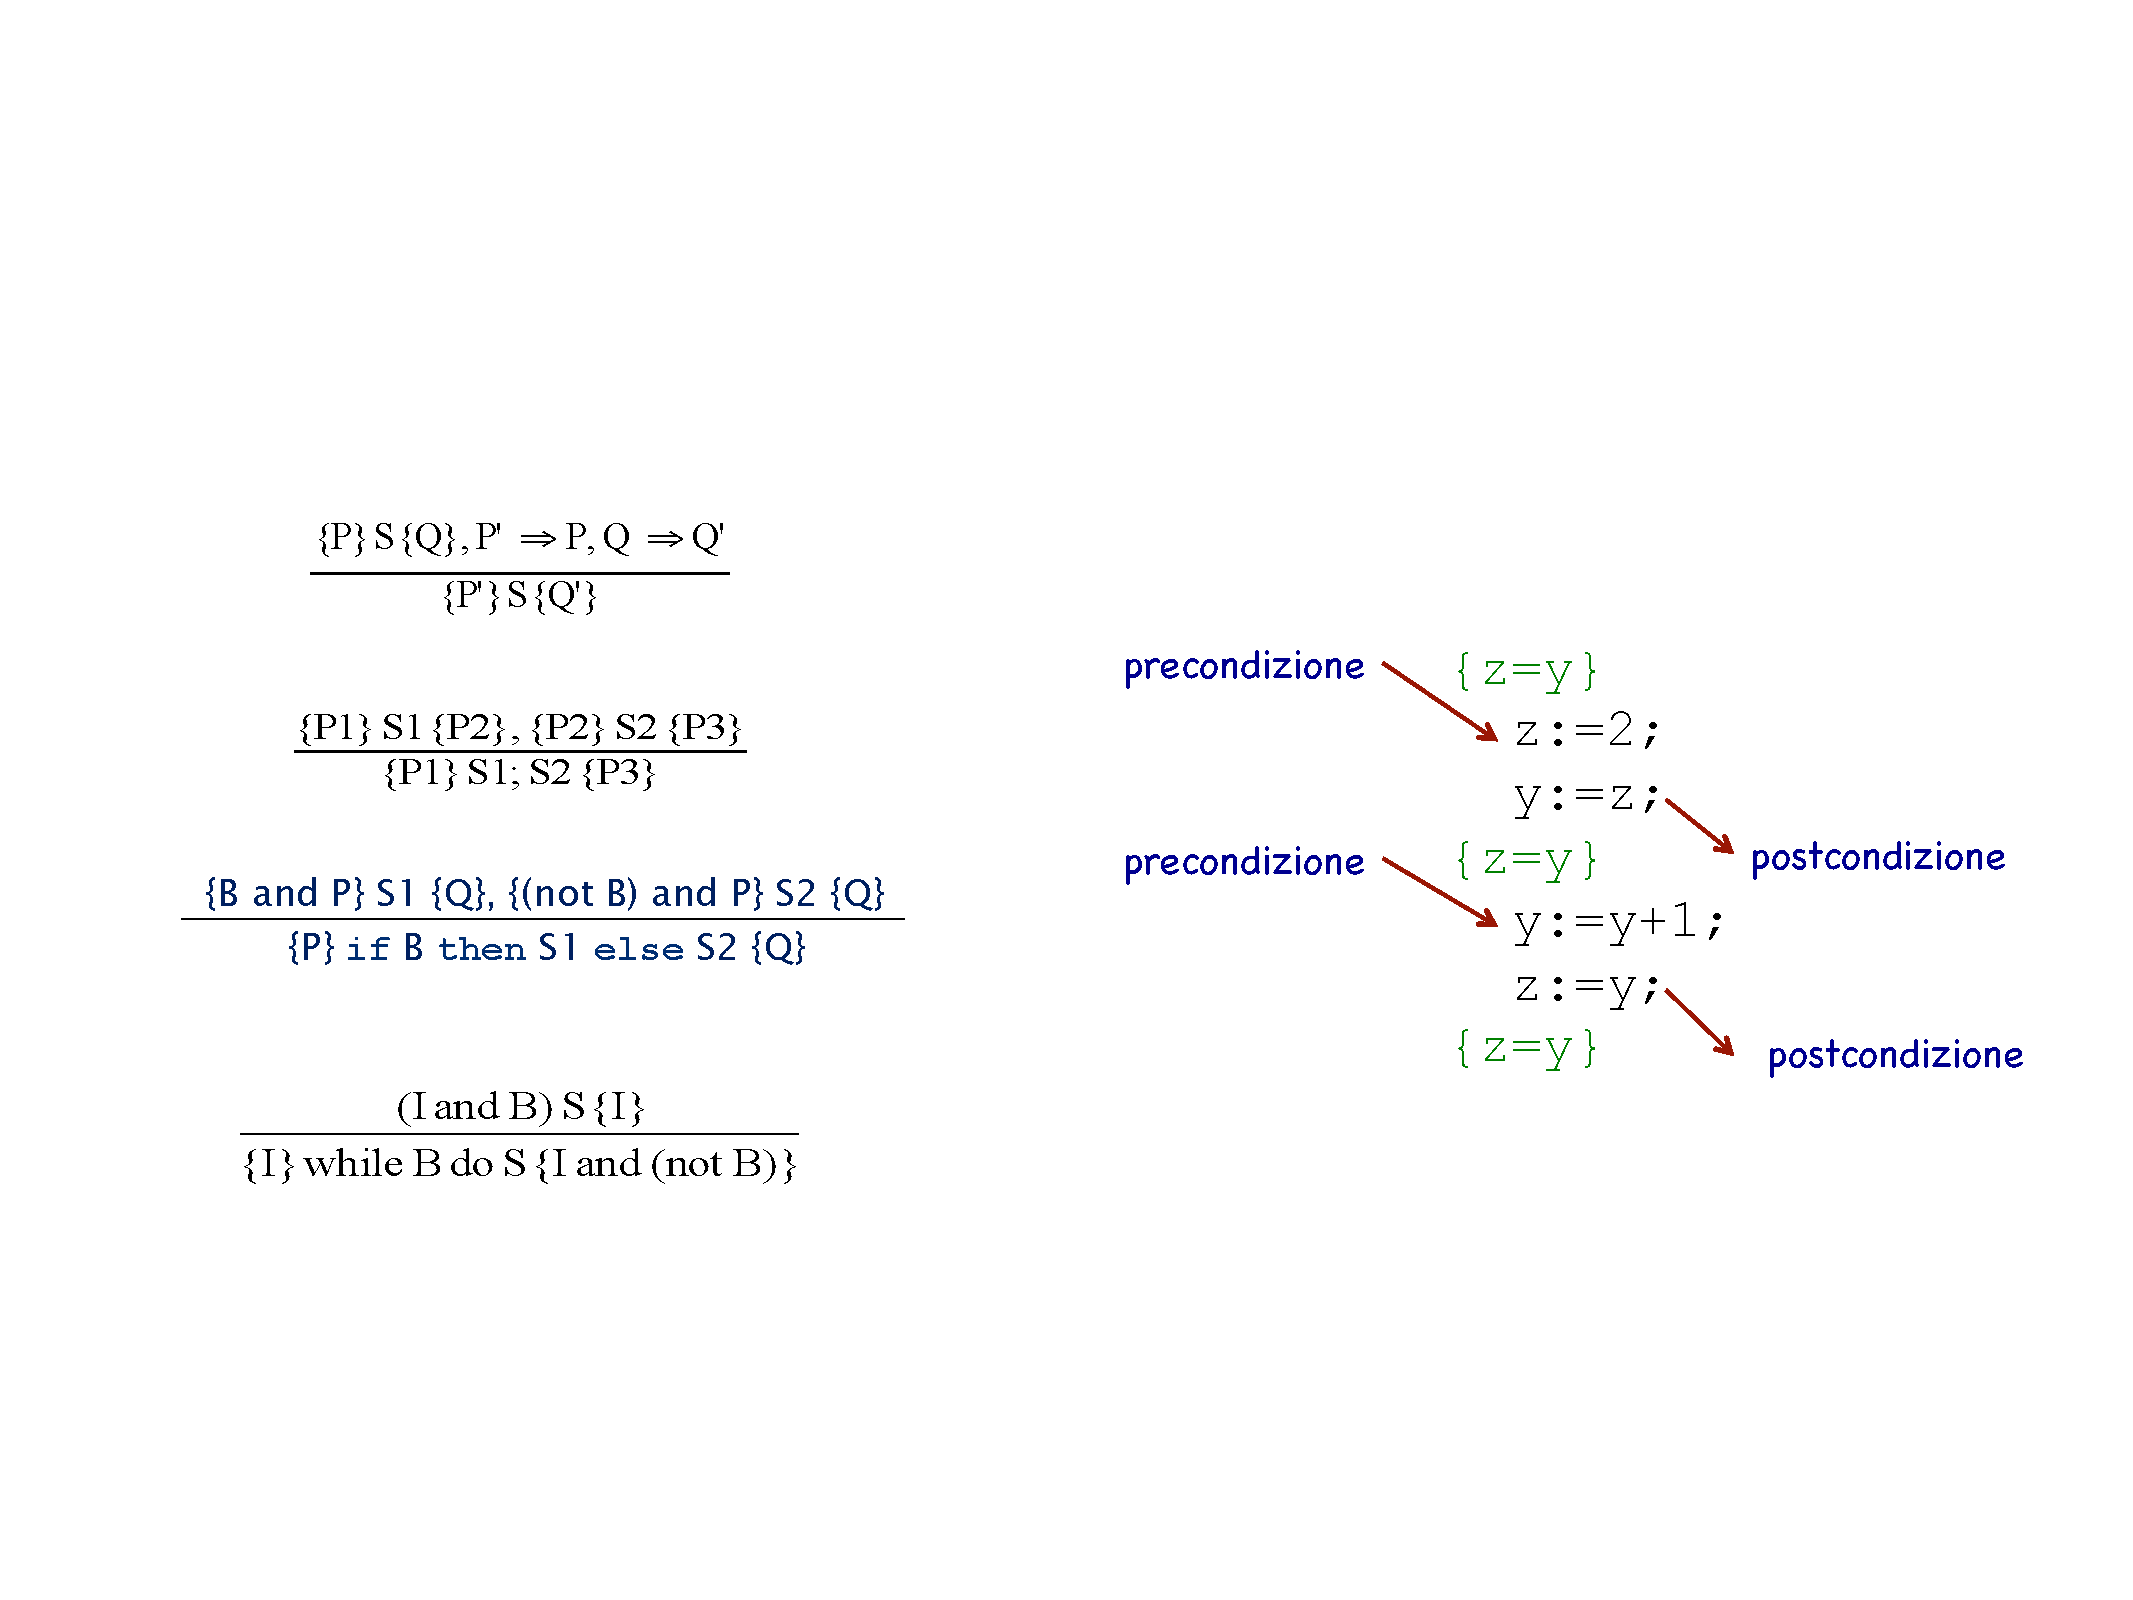
\includegraphics[width=\textwidth]{img/eg-semantica_assiomatica.pdf}
	\end{figure}\newpage

	\subsubsection{Semantica operazionale}
	
	\begin{boxdef}
		La \textcolor{Red3}{\textbf{semantica operazionale}} è un modello matematico dei programmi basato sui sistemi di transizione.
	\end{boxdef}
	
	\noindent
	La semantica operazionale descrive il significato del programma \textbf{eseguendo i suoi comandi su una macchina}, simulata o reale. La \textbf{trasformazione dello stato definisce il significato del comando}. Quindi, lo stato è la rappresentazione astratta della macchina.
	
	Inoltre, la semantica operazionale è necessaria per definire una macchina astratta.\newline
	
	\noindent
	Il modello matematico utilizzato è quello dei sistemi di transizione. Per \textcolor{Green4}{\textbf{esempio}}, si consideri la funzione memoria $\sigma: \mathrm{Var} \rightarrow \mathrm{Val}$ che associa valori alle variabili. Con \textbf{stato} si identifica una coppia nel programma ancora da eseguire:
	\begin{equation*}
		\mathrm{Stato} = \left\langle P,\sigma \right\rangle
	\end{equation*}
	Ad ogni passo, viene eseguita un'operazione e la configurazione o stato cambia. La chiusura transitiva descrive l'esecuzione completa.\newline
	Inoltre, questa semantica esegue i comandi separai da \dquotes{;} sequenzialmente e nell'ordine in cui compaiono da sinistra a destra.
	
	Infine, nonostante sia una delle forme più concrete di semantica, viene eseguita comunque un'astrazione di come il programma viene eseguito, quindi essa è indipendente dall'architettura.\newline
	
	\noindent
	Per \textcolor{Green4}{\textbf{esempio}}, il programma $P$ è formato nel seguente modo:
	\begin{lstlisting}[language=C]
		P:
		z := 2;
		y := z;
		y := y+1;
		z := y;\end{lstlisting}
	\begin{gather*}
		\left\langle z \coloneq 2; \hspace{1em} y \coloneq z; \hspace{1em} y \coloneq y+1; \hspace{1em} z \coloneq y, \left[z=\bot,y=\bot\right]\right\rangle \\
		\left\langle y \coloneq z; \hspace{1em} y \coloneq y+1; \hspace{1em} z \coloneq y, \left[z=2,y=\bot\right]\right\rangle \\		
		\left\langle y \coloneq y+1; \hspace{1em} z \coloneq y, \left[z=2,y=2\right]\right\rangle \\
		\left\langle z \coloneq y, \left[z=2,y=3\right]\right\rangle \\
		\left\langle \varepsilon, \left[z=3,y=3\right]\right\rangle
	\end{gather*}\newpage
	
	\subsubsection{Composizionalità}
	
	\begin{boxdef}
		La \textcolor{Red3}{\textbf{composizionalità}} è la proprietà per cui il significato di ogni programma deve essere in funzione del significato dei costituenti immediati.
	\end{boxdef}
	
	\noindent
	La composizionalità è una \textbf{proprietà della semantica} necessaria per caratterizzare i comportamenti e significati di sistemi che possono avere infiniti elementi.\newline
	
	\noindent
	L'\textbf{importanza} della composizionalità è dovuta alla necessità di analizzare le proprietà di un programma. Infatti, per farlo è necessario capire che cosa fa e dunque capire la semantica in ogni sua forma. L'analisi diventa molto più semplice grazie alla \textbf{modularità}, la quale è \textbf{garantita dalla composizionalità}. Quindi, anche nei software di grandi dimensioni, è possibile analizzare il codice separatamente nei suoi moduli, per poi ricomporre il risultato dell'analisi componendo i risultati ottenuti sui singoli moduli.
	
	\longline
	
	\subsubsection{Equivalenza}
	
	\begin{boxdef}
		L'\textcolor{Red3}{\textbf{equivalenza}} è vera quando due programmi hanno la stessa semantica.
	\end{boxdef}
	
	\noindent
	Per capire se due programmi sono equivalenti, viene osservata la relazione tra input e output. Se la relazione è la stessa, indipendentemente da come l'algoritmo la calcola, allora sono equivalenti. Quindi, solo caratterizzando la funzionalità I/O è possibile determinare questa caratteristica.\newline
	
	\noindent
	Infine, l'equivalenza è necessaria in varie fasi di analisi:
	\begin{itemize}
		\item \textbf{Correttezza}, per dimostrare che il programma scritto calcola esattamente la funzione attesa;
		
		\item \textbf{Equivalenza di programmi}, per dimostrare che due programmi calcolano la stessa funzione;
		
		\item \textbf{Efficienza}, Dati due programmi che calcolano la stessa funzione, si vuole dimostrare quale lo fa in modo più efficiente.
	\end{itemize}\newpage
	
	\subsection{Sintassi}
	
	\subsubsection{Stato (ambiente e memoria)}
	
	Per descrivere il significato dei programmi, è necessario introdurre due entità fondamentali: ambiente e memoria.\newline
	
	\noindent
	\begin{boxdef}
		L'\textcolor{Red3}{\textbf{ambiente}} (\textbf{\emph{environment}}) \textbf{è un insieme di legami (\emph{bindings}) tra identificatori e denotazioni}.
	\end{boxdef}
	Inoltre, l'ambiente specifica quali nomi sono usati e per quali oggetti, solitamente possono essere legati ad un tipo, ad un valore, ad una locazione. Quindi, i \emph{binding}\footnote{In breve sarebbero le API (\emph{Application Programming Interface}): \href{https://en.wikipedia.org/wiki/Language_binding}{link fonte}.} sono associati ai nomi, i quali possono essere variabili, costanti, procedure, e altro. I nomi sono solo un'entità separata dall'oggetto che denotano, infatti esso potrebbe essere usato in contesti diversi per rappresentare valori differenti.\newline
	
	\noindent
	\begin{boxdef}
		La \textcolor{Red3}{\textbf{memoria}} (\textbf{\emph{store}}) \textbf{è un insieme di effetti sugli identificatori (causati da assegnamenti)}.
	\end{boxdef}
	Essa è una mappa che solitamente rappresenta la storia, cioè l'evoluzione, delle variazioni dei valori associati agli identificatori. In altre parole, fornisce un \emph{binding} tra locazione e valore.\newline
	Si ricorda, che la memoria è fortemente legato all'approccio imperativo, infatti i linguaggi funzionali pure non ne hanno bisogno dato che non gestiscono variabili che cambiano durante l'esecuzione del programma.
	
	\longline
	
	\subsubsection{Categorie sintattiche}
	
	\begin{boxdef}
		Le \textcolor{Red3}{\textbf{categorie sintattiche}} \textbf{sono la classificazione dei costrutti in funzione del loro significato atteso, ovvero della classe di effetti che ha la loro esecuzione causa.}
	\end{boxdef}
	Quindi, esse sono classi che rappresentano un diverso tipo di significato, effetto, esecuzione di un programma.\newline
	
	\noindent
	Le categorie sintattiche si distinguono in: \textbf{espressioni}, \textbf{comandi} e \textbf{dichiarazioni}. Formalmente, le categorie sono i simboli non terminali della grammatica classificati in funzione di cosa modificano dello stato e come lo modificano.\newpage
	
	\subsubsection{Espressioni}
	
	Le \textcolor{Red3}{\textbf{espressioni}} \textbf{nascono dalla necessità di avere una categoria sintattica che consenta di rappresentare e denotare i valori}. Esse possono essere espresse con dei vincoli, per esempio il tipo.\newline
	
	\noindent
	Nonostante le espressioni denotino i valori, esse \textbf{non sono locazioni di memoria}. Quest'ultime sono legati all'architettura (struttura) di una macchina, mentre le espressioni fanno riferimento allo specifico linguaggio di programmazione.\newline
	
	\noindent
	\begin{boxdef}
		Due espressioni sono considerate \textcolor{Red3}{\textbf{equivalenti}} \textbf{se vengono valutate nello stesso valore in tutti gli stati di computazione. Anche eventuali \emph{side-effect} devono essere gli stessi}.
	\end{boxdef}
	
	Infatti, due espressioni possono essere diverse ma essere valutate nello stesso valore. Per \textcolor{Green4}{\textbf{esempio}}, l'espressione logica \textsf{not(a and b)} è logicamente (semanticamente) equivalente ad \textsf{(not a) or (not b)} ma sono sintatticamente diverse.
	
	\longline
	
	\subsubsection{Dichiarazioni}
	
	Le \textcolor{Red3}{\textbf{dichiarazioni}} \textbf{sono la categoria sintattica che consente la creazione o la modifica dei legami associati agli identificatori, ovvero gli ambienti}.\newline
	
	\noindent
	Esse nascono con l'obbiettivo di utilizzare i valori. Per farlo, è stato necessario creare, utilizzare e modificare \textbf{legami} tra nomi e valori.\newline
	
	\noindent
	Inoltre, gli le modifiche agli ambienti sono trasformazioni \textbf{reversibili}, ovvero che le trasformazioni hanno valenza esclusivamente all'interno del raggio d'azione (\emph{scope}) attuale dell'identificatore. In altre parole, i linguaggi di programmazione delimitano la validità di un ambiente. Più precisamente con \textbf{reversibili si intende} che una volta terminata la validità di un ambiente, le modifiche verranno annullate.\newline
	
	\noindent
	\begin{boxdef}
		Due dichiarazioni sono \textcolor{Red3}{\textbf{equivalenti}} \textbf{se producono lo stesso ambiente e la stessa memoria in caso di \emph{side-effect} in tutti gli stati di computazione}.
	\end{boxdef}
	A causa del \emph{side-effect} è necessario che l'equivalenza richieda che due dichiarazioni generino le stesse identiche modifiche a tutto lo stato di computazione.\newpage
	
	\subsubsection{Comandi}
	
	I \textcolor{Red3}{\textbf{comandi}} \textbf{sono richieste di modifica dello stato di computazione, ed in particolare della memoria}.\newline
	
	\noindent
	Le trasformazioni sono \textbf{irreversibili}, ovvero sono definite nell'esecuzione del programma. Quindi, per annullarle è necessario eseguire altri comandi e altre trasformazioni che consentono di tornare alla stessa memoria iniziale. Quindi, i comandi non sono altro che funzioni di trasformazione e devono essere \textbf{eseguiti} per poter attuare la corrispondente trasformazione (irreversibile) della memoria.
	
	\begin{boxdef}
		Due comandi sono \textcolor{Red3}{\textbf{equivalenti}} \textbf{se per ogni stato (memoria) in input producono lo stesso stato (memoria) in output}.
	\end{boxdef}

	\longline

	\subsection{Semantica operazionale: sistemi di transizione}
	
	I \textcolor{Red3}{\textbf{sistemi di transizione}} \textbf{sono strumenti astratti mirati a specificare senza ambiguità e senza dipendenza dalla macchina, cosa fa un linguaggio}. Le sue caratteristiche principali sono:
	\begin{itemize}
		\item Matematicamente precisi;

		\item Molto concisi;

		\item Metodo di specifica generale che consente l'astrazione;

		\item Specificano cosa viene calcolato per induzione sulla struttura sintattica del linguaggio.
	\end{itemize}
	Inoltre, sfruttando la definizione induttiva del linguaggio, consentono di definire il significato mediante induzione sull'\emph{abstract syntax tree}. Quindi, viene \textbf{usata l'induzione strutturale matematica per ragion sui programmi}.\newline
	
	\noindent
	\begin{boxdef}
		Formalmente: \textbf{un \textcolor{Red3}{sistema di transizione} è una struttura $\left(\Gamma, \rightarrow\right)$, dove $\Gamma$ è un insieme di elementi $\gamma$ chiamati configurazioni e la relazione binaria $\rightarrow \subseteq \Gamma \times \Gamma$ è chiamata relazione di transizione. Se $\Gamma_{T} \subseteq \Gamma$ è un insieme di configurazioni terminali, il sistema è detto terminale.}
	\end{boxdef}\newpage
	
	\subsection{Esempio di un linguaggio reale ($PL_{0}$)}\label{esempio di un linguaggio reale PL0}
	
	Un esempio di linguaggio reale è $PL_{0}$ strutturato nel seguente modo:
	\begin{figure}[!htp]
		\centering
		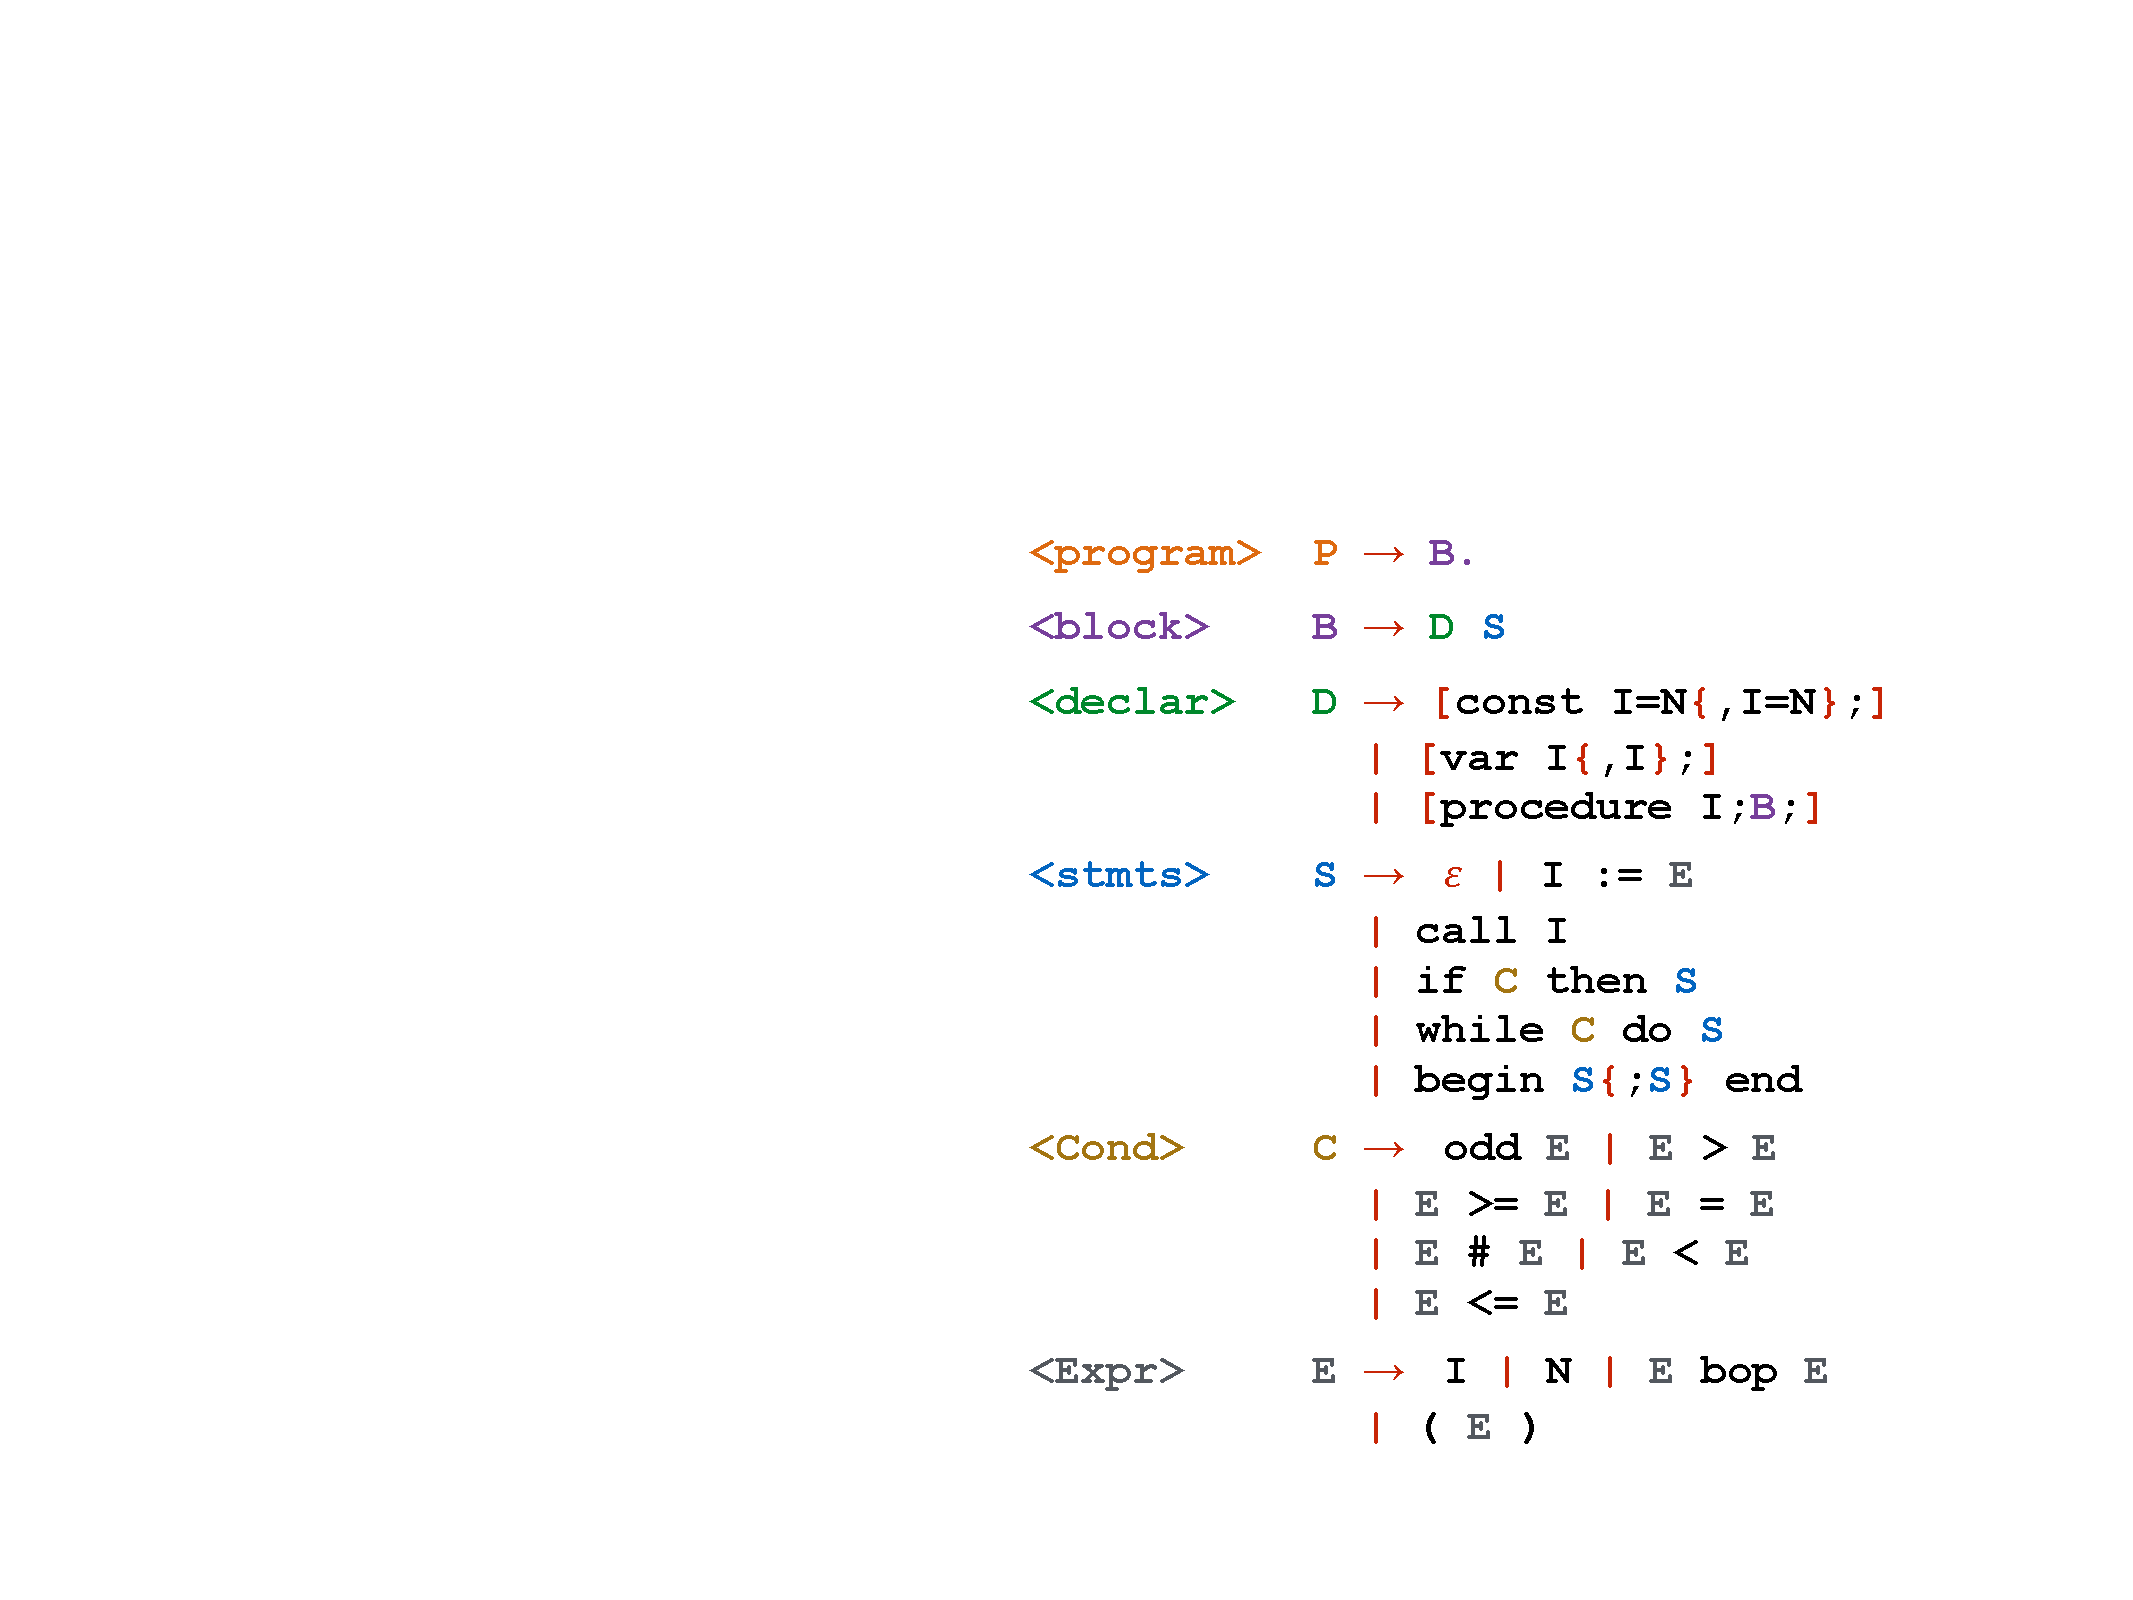
\includegraphics[width=.6\textwidth]{img/pl0.pdf}
	\end{figure}
	
	\begin{itemize}
		\item I programmi $P$ sono blocchi.
		
		\item I blocchi $B$ sono una dichiarazione $D$ seguita da un comando $S$, entrambi liberi dal contesto.
		
		\item Le dichiarazioni $D$ sono dichiarazioni di valori costanti con nome (const), dichiarazioni di variabili (var) e dichiarazioni di procedure.
		
		\item I nomi sono gli identificatori $I$, considerati parte del vocabolario, e $N$ sono i numeri naturali, anch'essi considerati parte del vocabolario.
		
		\item Non esiste il concetto di tipo poiché l'unico dato ammesso è intero.
		
		\item I comandi sono:
		\begin{itemize}
			\item Comando vuoto;
			\item Assegnamento di un valore ad un identificatore;
			\item Chiamata ad una procedura mediante il suo nome;
			\item Comando condizionale che esegue un comando al verificarsi di una condizione booleana;
			\item Ciclo che ripete un comando finché una data condizione è vera;
			\item Composizione sequenziale di comandi.
		\end{itemize}
	
		\item Le condizioni $C$ sono espressioni che hanno al loro interno valori booleani.
		
		\item Le espressioni $E$ sono identificatori, valori naturali, operazioni tra espressioni e espressioni tra parentesi.
	\end{itemize}\newpage

	\section{Espressioni}
	
	\subsection{Introduzioni}
	
	Per manipolare i valori è necessario rappresentarli e per questo motivo vengono utilizzate le espressioni. Quest'ultime, devono essere valutate per dare un valore e con valore non viene intesa la locazione di memoria: i valori fanno parte dello specifico linguaggio di programmazione, mentre la locazione è parte della struttura dell'architettura. Quindi, la locazione di memoria modella il modo in cui il linguaggio di programmazione si relazione alla macchina sottostante.
	
	\longline
	
	\subsection{Descrivere le espressioni}
	
	Per associare significati e valori alle \textbf{espressioni}, esse \textbf{devono essere valutate}.\newline
	
	\noindent
	Il \textbf{valore ottenuto mediante la valutazione} è chiamato \textbf{valore esprimibile}, poiché è un \textbf{valore che può essere espresso attraverso la sintassi del linguaggio di programmazione}, e in particolare attraverso la sintassi delle espressioni.\newline
	
	\noindent
	\textbf{Formalmente} con \textcolor{Red3}{\textbf{valore esprimibile}} si intende l'unione tra i tipi booleani e interi:
	\begin{equation*}
		Eval = bool \cup int \hspace{2em} \text{con metavariabile } ev
	\end{equation*}
	Per metavariabile si intende qualsiasi valore esprimibile.\newline
	
	\noindent
	Per \textcolor{Green4}{\textbf{esempio}}, un linguaggio come $PL_{0}$ (paragrafo \ref{esempio di un linguaggio reale PL0}), si hanno espressioni che rappresentano interi e identificatori, e indirettamente anche booleani in quanto le condizioni corrispondono a valori booleani (e.g. $3=3$ è \emph{true}, mentre $3\#3$ è \emph{false}).\newline
	
	\noindent
	Dal punto di vista \textbf{sintattico}, i \textbf{costituenti elementari delle espressioni} sono \textbf{letterali} (costanti e identificatori), i quali sono \textbf{composti mediante operatori}.\newline
	
	\noindent
	\textbf{Per concludere}, un'espressione è un oggetto sintattico composto da operatori, operandi (che sono espressioni alla fine), parentesi e funzioni/procedure.\newpage
	
	\subsection{Caratteristiche}
	
	Ecco qua di seguito gli \textbf{aspetti che caratterizzano le espressioni}:
	\begin{itemize}
		\item \textcolor{Red3}{\textbf{Notazione}} che specifica in che modo gli operandi e gli operatori vengono rappresentati. Inoltre, indica su quali operandi un operatore opera.
		\begin{itemize}
			\item Paragrafo \ref{notazione} sulla notazione
			\item Paragrafo \ref{notazione post-fissa} sulla notazione post-fissa
			\item Paragrafo \ref{notazione pre-fissa} sulla notazione pre-fissa
			\item Paragrafo \ref{notazione in-fissa} sulla notazione in-fissa
		\end{itemize}
		
		\item \textcolor{Red3}{\textbf{Regole di precedenza}} tra operatori
		
		\item \textcolor{Red3}{\textbf{Regole di associatività}} degli operatori
		
		\item \textcolor{Red3}{\textbf{Ordine di valutazione degli operandi}}
		
		\item \textcolor{Red3}{\textbf{Presenza di \emph{side-effects}}}, ovvero qualunque effetto che non consiste puramente nella rappresentazione di valori;
		
		\item \textcolor{Red3}{\textbf{\emph{Overloading} degli operatori}}, ovvero simboli di operatori che hanno significati diversi a seconda del tipo degli operatori a cui sono applicati.
		
		\item \textcolor{Red3}{\textbf{Espressioni con tipi misti}}
	\end{itemize}
	
	\longline
	
	\subsubsection{Notazione}\label{notazione}
	
	A seconda di \textbf{come viene rappresentata l'espressione}, \textbf{varia anche il modo in cui viene determinata la semantica} e di conseguenza varia la sua valutazione.\newline
	
	\noindent
	Esistono \textbf{diversi modi per denotare le espressioni}:
	\begin{itemize}
		\item Notazione \textbf{in-fissa}, per esempio $a+b$
		\item Notazione \textbf{pre-fissa} (polacca), per esempio $+ab$
		\item Notazione \textbf{post-fissa} (polacca inversa), per esempio $ab+$
	\end{itemize}
	La notazione in-fissa è quella più utilizza nelle espressioni aritmetiche poiché più intuitiva, ma sono necessarie altre regole per eliminare l'ambiguità. Nelle altre notazioni (pre e post fissa), l'\textcolor{Red3}{\textbf{arietà dell'operatore}}, ovvero il \textbf{numero di operandi a cui si applica}, è spesso sufficiente ad evitare ambiguità nella valutazione.\newpage
	
	\subsubsection{Notazione post-fissa}\label{notazione post-fissa}
	
	La notazione \textcolor{Red3}{\textbf{post-fissa}} è \textbf{più semplice della in-fissa}, dal punto di vista della \textbf{computazione}, poiché:
	\begin{itemize}
		\item Non sono necessarie regole di precedenza
		\item Non sono necessarie regole di associatività
		\item Non sono necessarie parentesi
	\end{itemize}
	Viene anche concessa una rappresentazione uniforme per qualsiasi arietà di operatori\footnote{Arietà: numero di operandi a cui si applica.}.\newline
	
	\noindent
	Vengono presentati due \textcolor{Green4}{\textbf{esempi}}:
	\begin{itemize}
		\item La notazione $ab+cd+*$ viene valutata da sinistra a destra usando una pila LIFO (\emph{Last In, First Out}).
		
		\item La notazione $532*+$ viene valutata nel seguente modo: durante la lettura, i valori vengono messi sulla pila; nel momento in cui viene trovato un operatore, come $*$, sapendo che la sua arietà è $2$, è noto che l'operatore viene applicato ai primi due valori in cima alla pila. Infine, il risultato dopo ogni operazione viene caricato in cima alla pila;
	\end{itemize}
	L'\textcolor{Red3}{\textbf{algoritmo di valutazione}} si articola in pochi passaggi. \textbf{Graficamente è possibile leggerlo nella prossima pagina}, mentre in forma scritta qui di seguito:
	\begin{enumerate}
		\item Lettura di un simbolo dall'espressione.
		
		\begin{enumerate}
			\item Se il simbolo letto è un operatore:
			\begin{enumerate}
				\item Applicazione dell'operatore a $n$ operandi immediatamente precedente sulla pila, il numero di operandi dipende dall'arietà dell'operatore.
				
				\item Memorizzazione del risultato in $R$.
				
				\item Eliminazione dell'operatore e degli operandi dalla pila.
				
				\item Memorizzazione del valore $R$ sulla pila.
			\end{enumerate}
			
			\item Se il simbolo letto non è un operatore, allora è un operando e viene inserito direttamente in pila.
		\end{enumerate}
		
		\item Se ci sono altri simboli da leggere rinizia dal punto 1, altrimenti termina e il risultato sarà in cima alla pila.
	\end{enumerate}\newpage

	\begin{figure}[!htp]
		\centering
		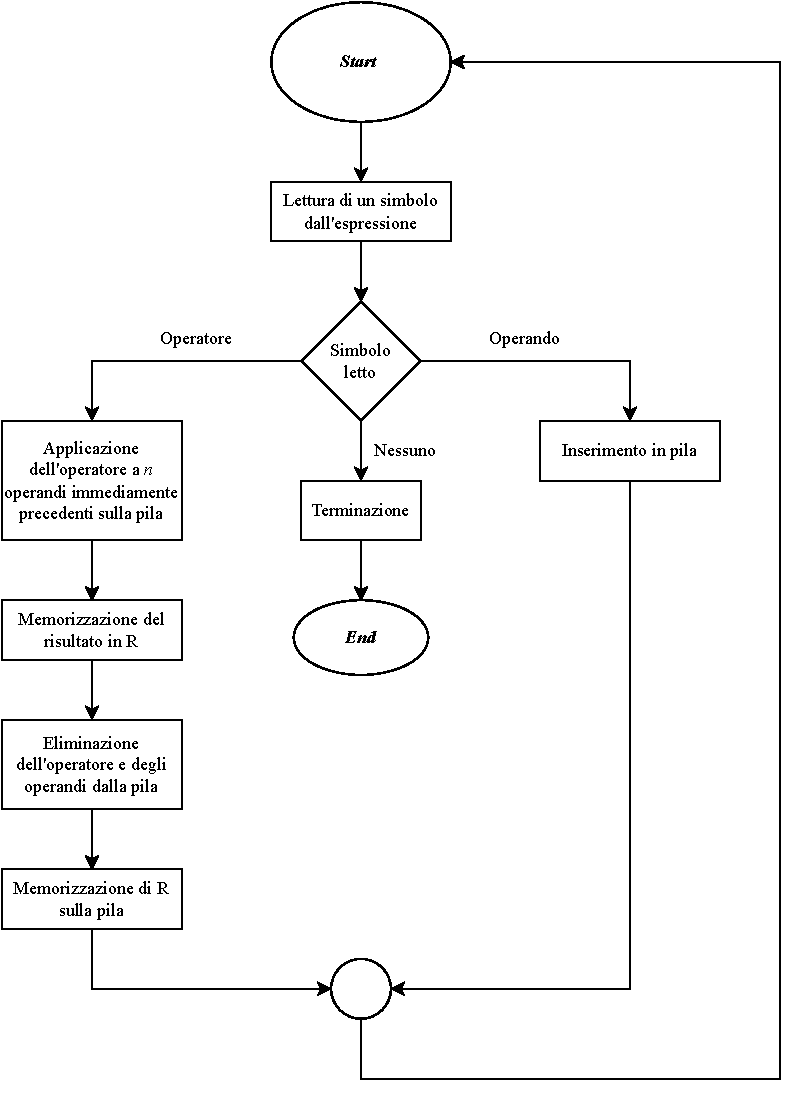
\includegraphics[width=\textwidth]{img/algoritmo_notazione_post-fissa.pdf}
		\caption{Algoritmo di valutazione nella notazione post-fissa.}
	\end{figure}\newpage

	\begin{figure}[!htp]
		\centering
		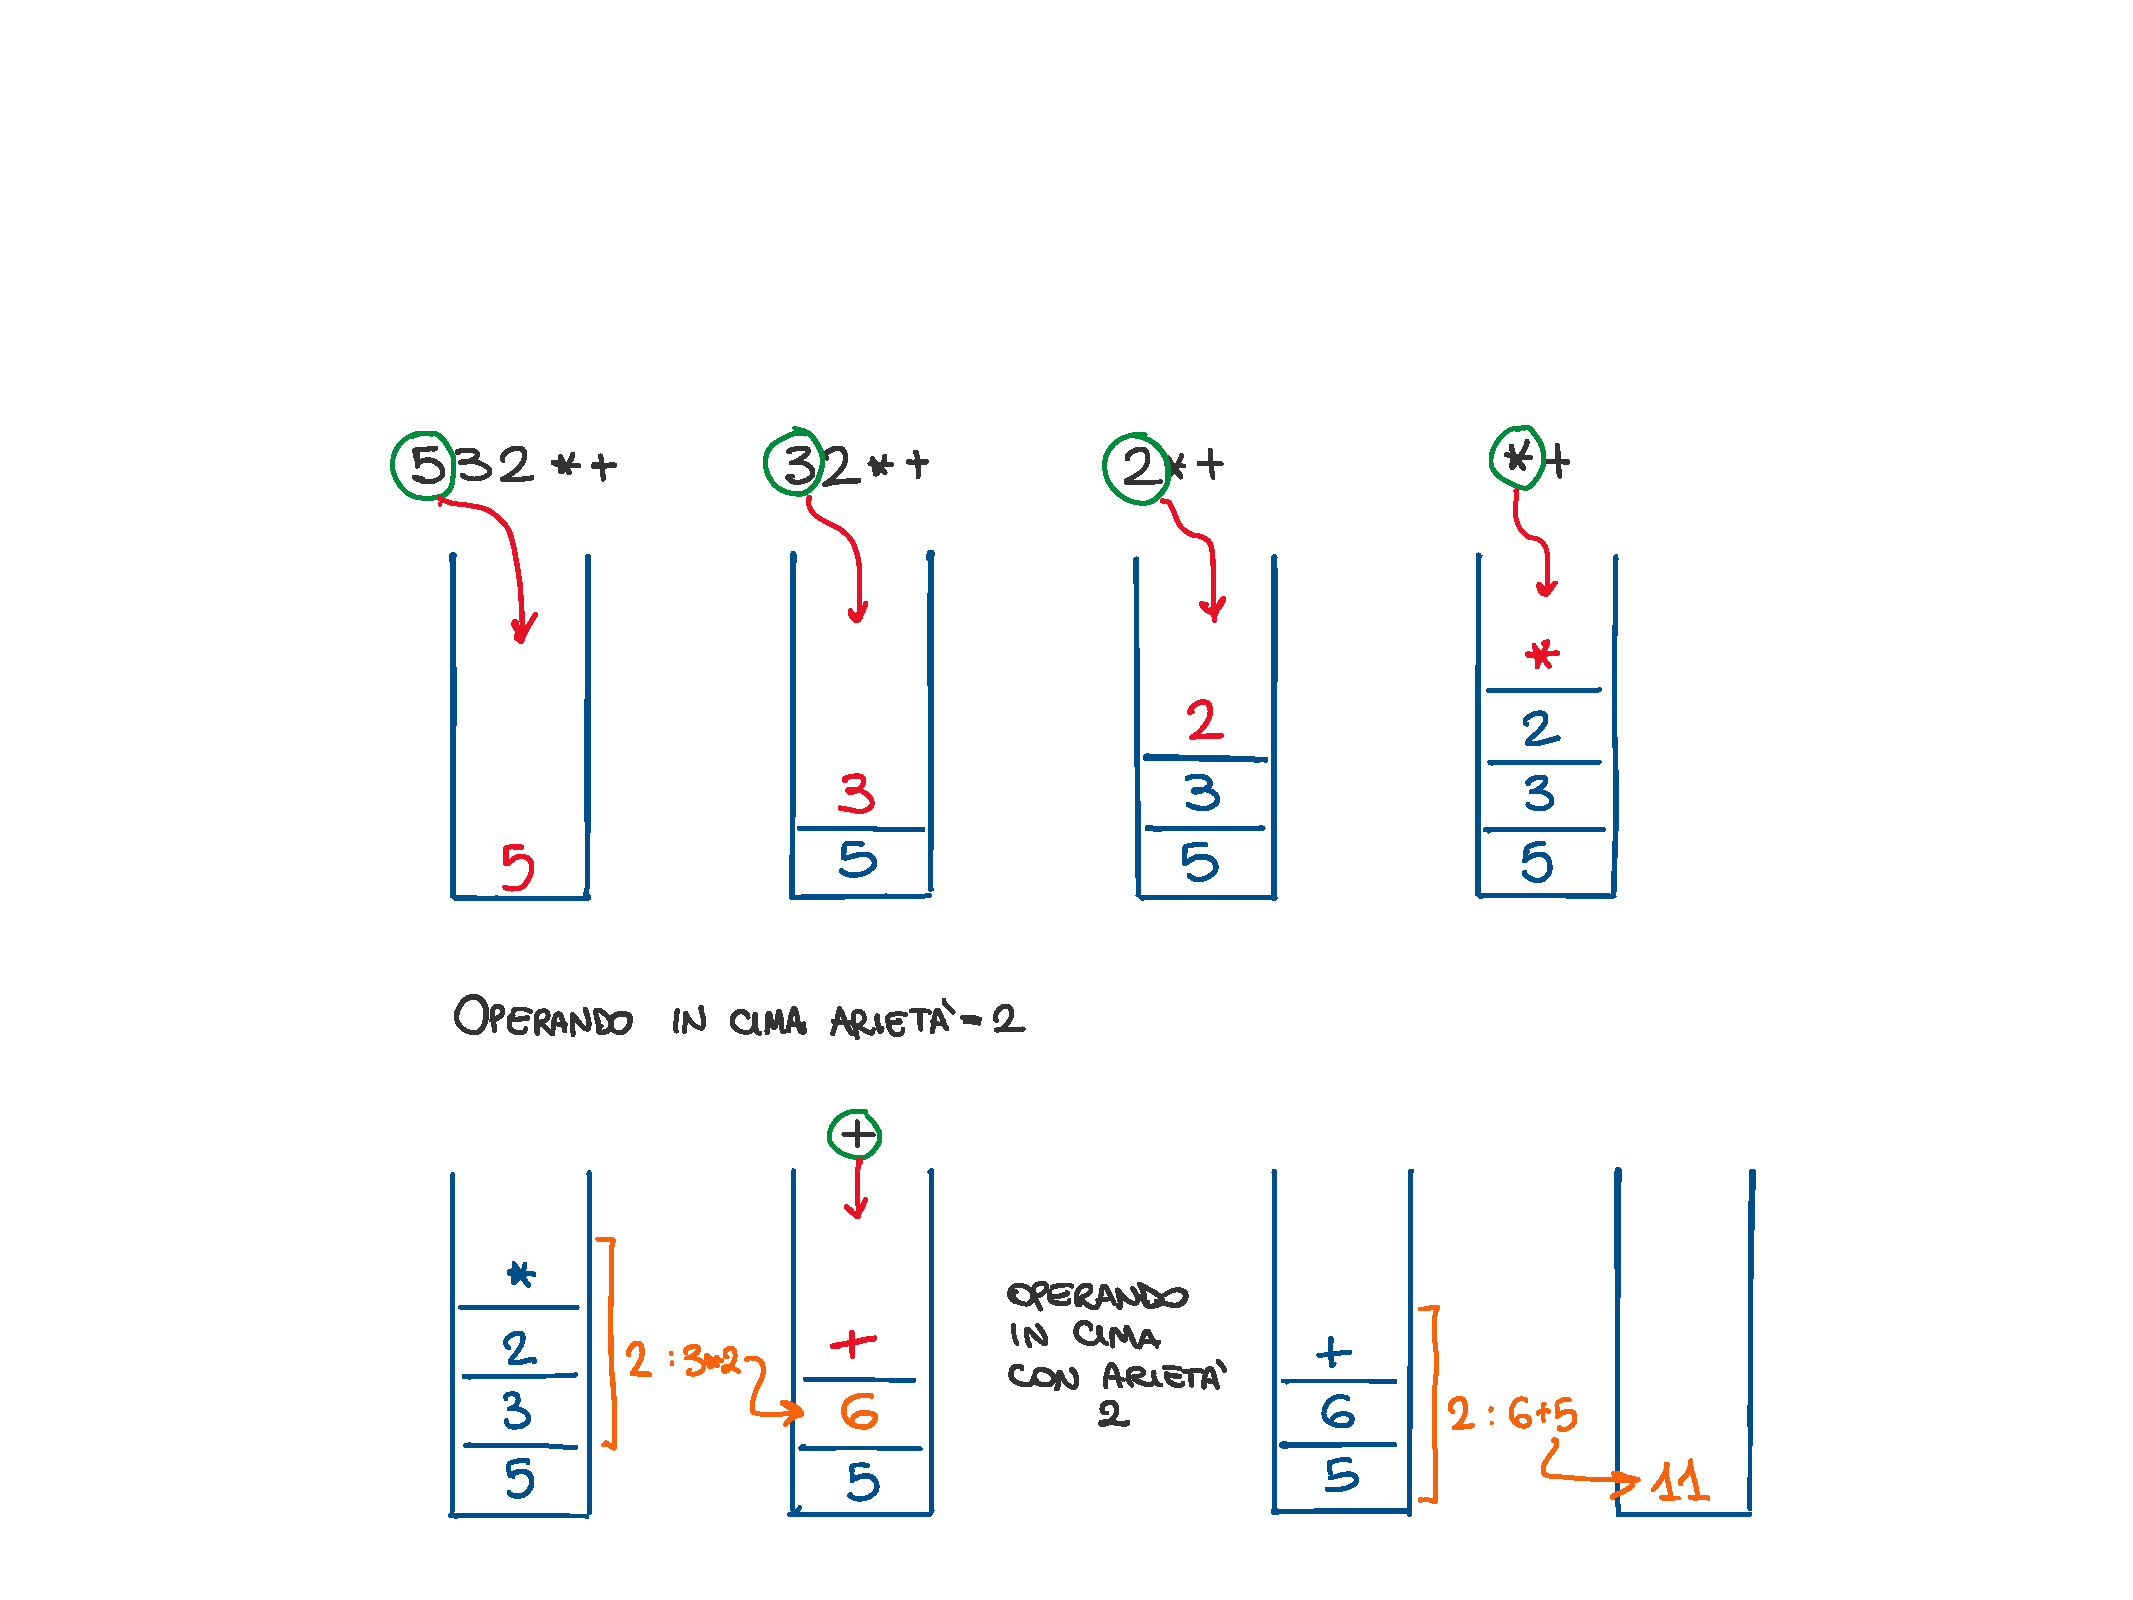
\includegraphics[width=\textwidth]{img/esempio_notazione_post-fissa.pdf}
		\caption{Esempio di applicazione dell'algoritmo di valutazione della notazione post-fissa.}
	\end{figure}\newpage
	
	\subsubsection{Notazione pre-fissa}\label{notazione pre-fissa}
	
	La notazione \textcolor{Red3}{\textbf{pre-fissa}} è \textbf{più semplice della in-fissa}, dal punto di vista della \textbf{computazione}, poiché:
	\begin{itemize}
		\item Non sono necessarie regole di precedenza
		\item Non sono necessarie regole di associatività
		\item Non sono necessarie parentesi
	\end{itemize}
	Viene anche concessa una rappresentazione uniforme per qualsiasi arietà di operatori\footnote{Arietà: numero di operandi a cui si applica.}.\newline
	
	\noindent
	A \textbf{differenza della notazione post-fissa}, l'\textbf{algoritmo} di valutazione è \textbf{più complicato} poiché è necessario contare gli operandi che vengono letti.\newline
	
	\noindent
	Per \textcolor{Green4}{\textbf{esempio}}, la notazione $*+ab+cd$ viene valutata da sinistra a destra usando una pila LIFO (\emph{Last In, First Out}). A differenza delle altre notazioni, in questo caso ogni volta che viene letto un operatore, è necessario contare gli operandi da leggere prima di eseguire il calcolo.\newline
	
	\noindent
	L'\textcolor{Red3}{\textbf{algoritmo di valutazione}} si articola in pochi passaggi. \textbf{Graficamente è possibile leggerlo nella prossima pagina}, mentre in forma scritta qui di seguito:
	\begin{enumerate}
		\item Lettura di un simbolo dall'espressione e inserimento in pila.
		
		\begin{enumerate}
			\item Se il simbolo letto è un operatore, inizializza il contatore $C$ con il numero di argomenti dell'operatore $\left(C_{op} = n\right)$ e torna al punto 1;
			
			\item Se il simbolo letto è un operando, decrementa il contatore $C$ di uno $\left(C_{op} = C_{op}-1\right)$ ($op$ è l'ultimo operatore inserito):
			
			\begin{enumerate}
				\item Se $C_{op} \ne 0$, torna al punto 1;
				
				\item Se $C_{op} = 0$ vengono eseguite le seguenti operazioni:
				
				\begin{enumerate}
					\item Applicazione dell'ultimo operatore agli operandi in cima alla pila;\newline
					memorizzazione del risultato in $R$;\newline
					eliminazione dell'operatore e degli operandi processati dalla pila;\newline
					memorizzazione del risultato $R$ sulla pila;
					
					\item Se non vi sono più simboli di operatore sulla pila, si salta al punto 2 (la fine);
					
					\item Inizializzazione del nuovo contatore: $C_{op} = n - m$ dove $n$ è l'arietà del nuovo operatore nella pila, il quale si trova in cima, e $m$ è il numero di operandi presenti nella pila sopra tale operatore;
					
					\item Ritorna al punto \emph{i}.
				\end{enumerate}
			\end{enumerate}
		\end{enumerate}
		
		\item Se la sequenza da leggere non è vuota torna all'1.
	\end{enumerate}\newpage
	
	\begin{figure}[!htp]
		\centering
		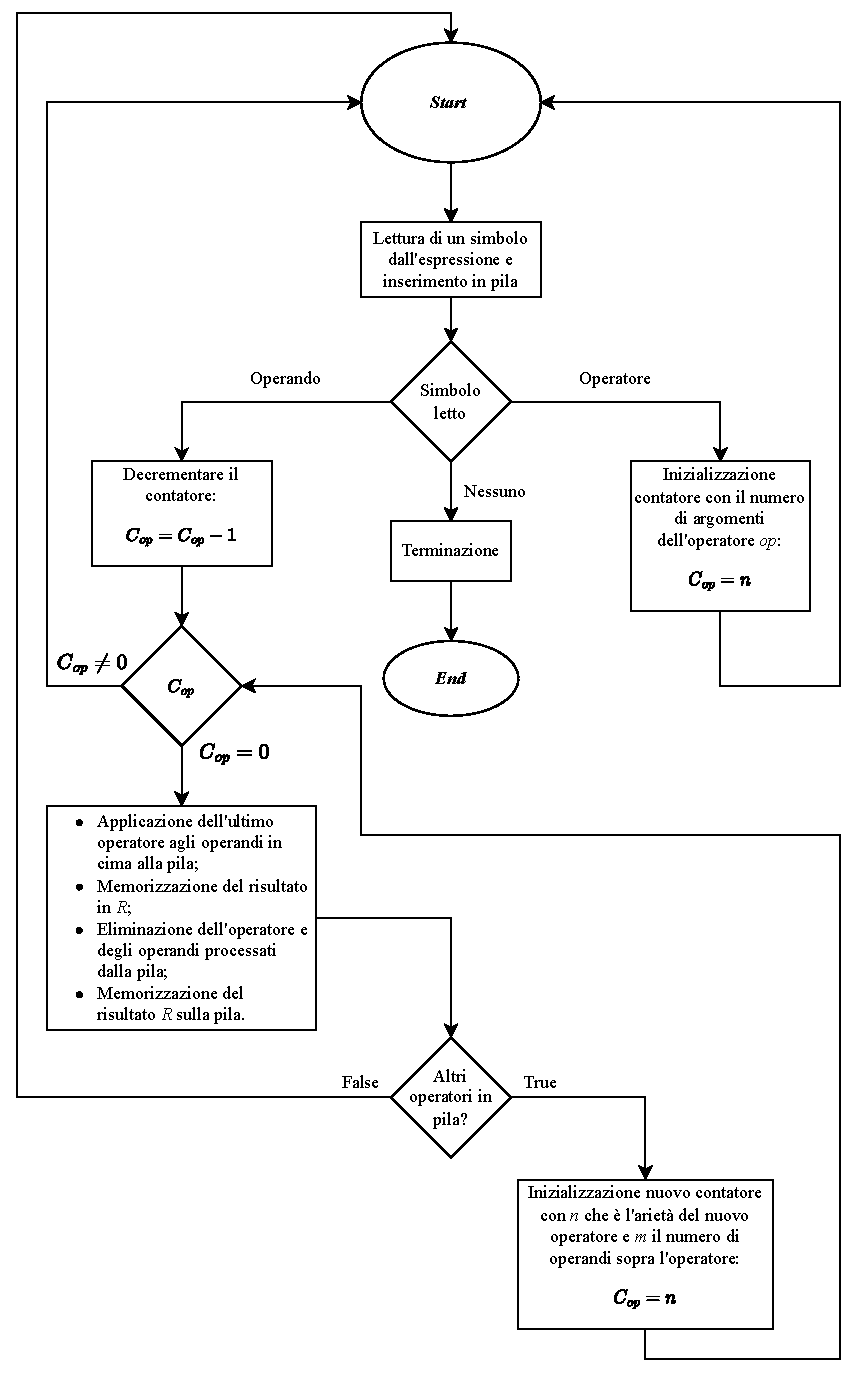
\includegraphics[width=\textwidth]{img/algoritmo_notazione_pre-fissa.pdf}
		\caption{Algoritmo di valutazione nella notazione post-fissa.}
	\end{figure}\newpage
	
	\begin{figure}[!htp]
		\centering
		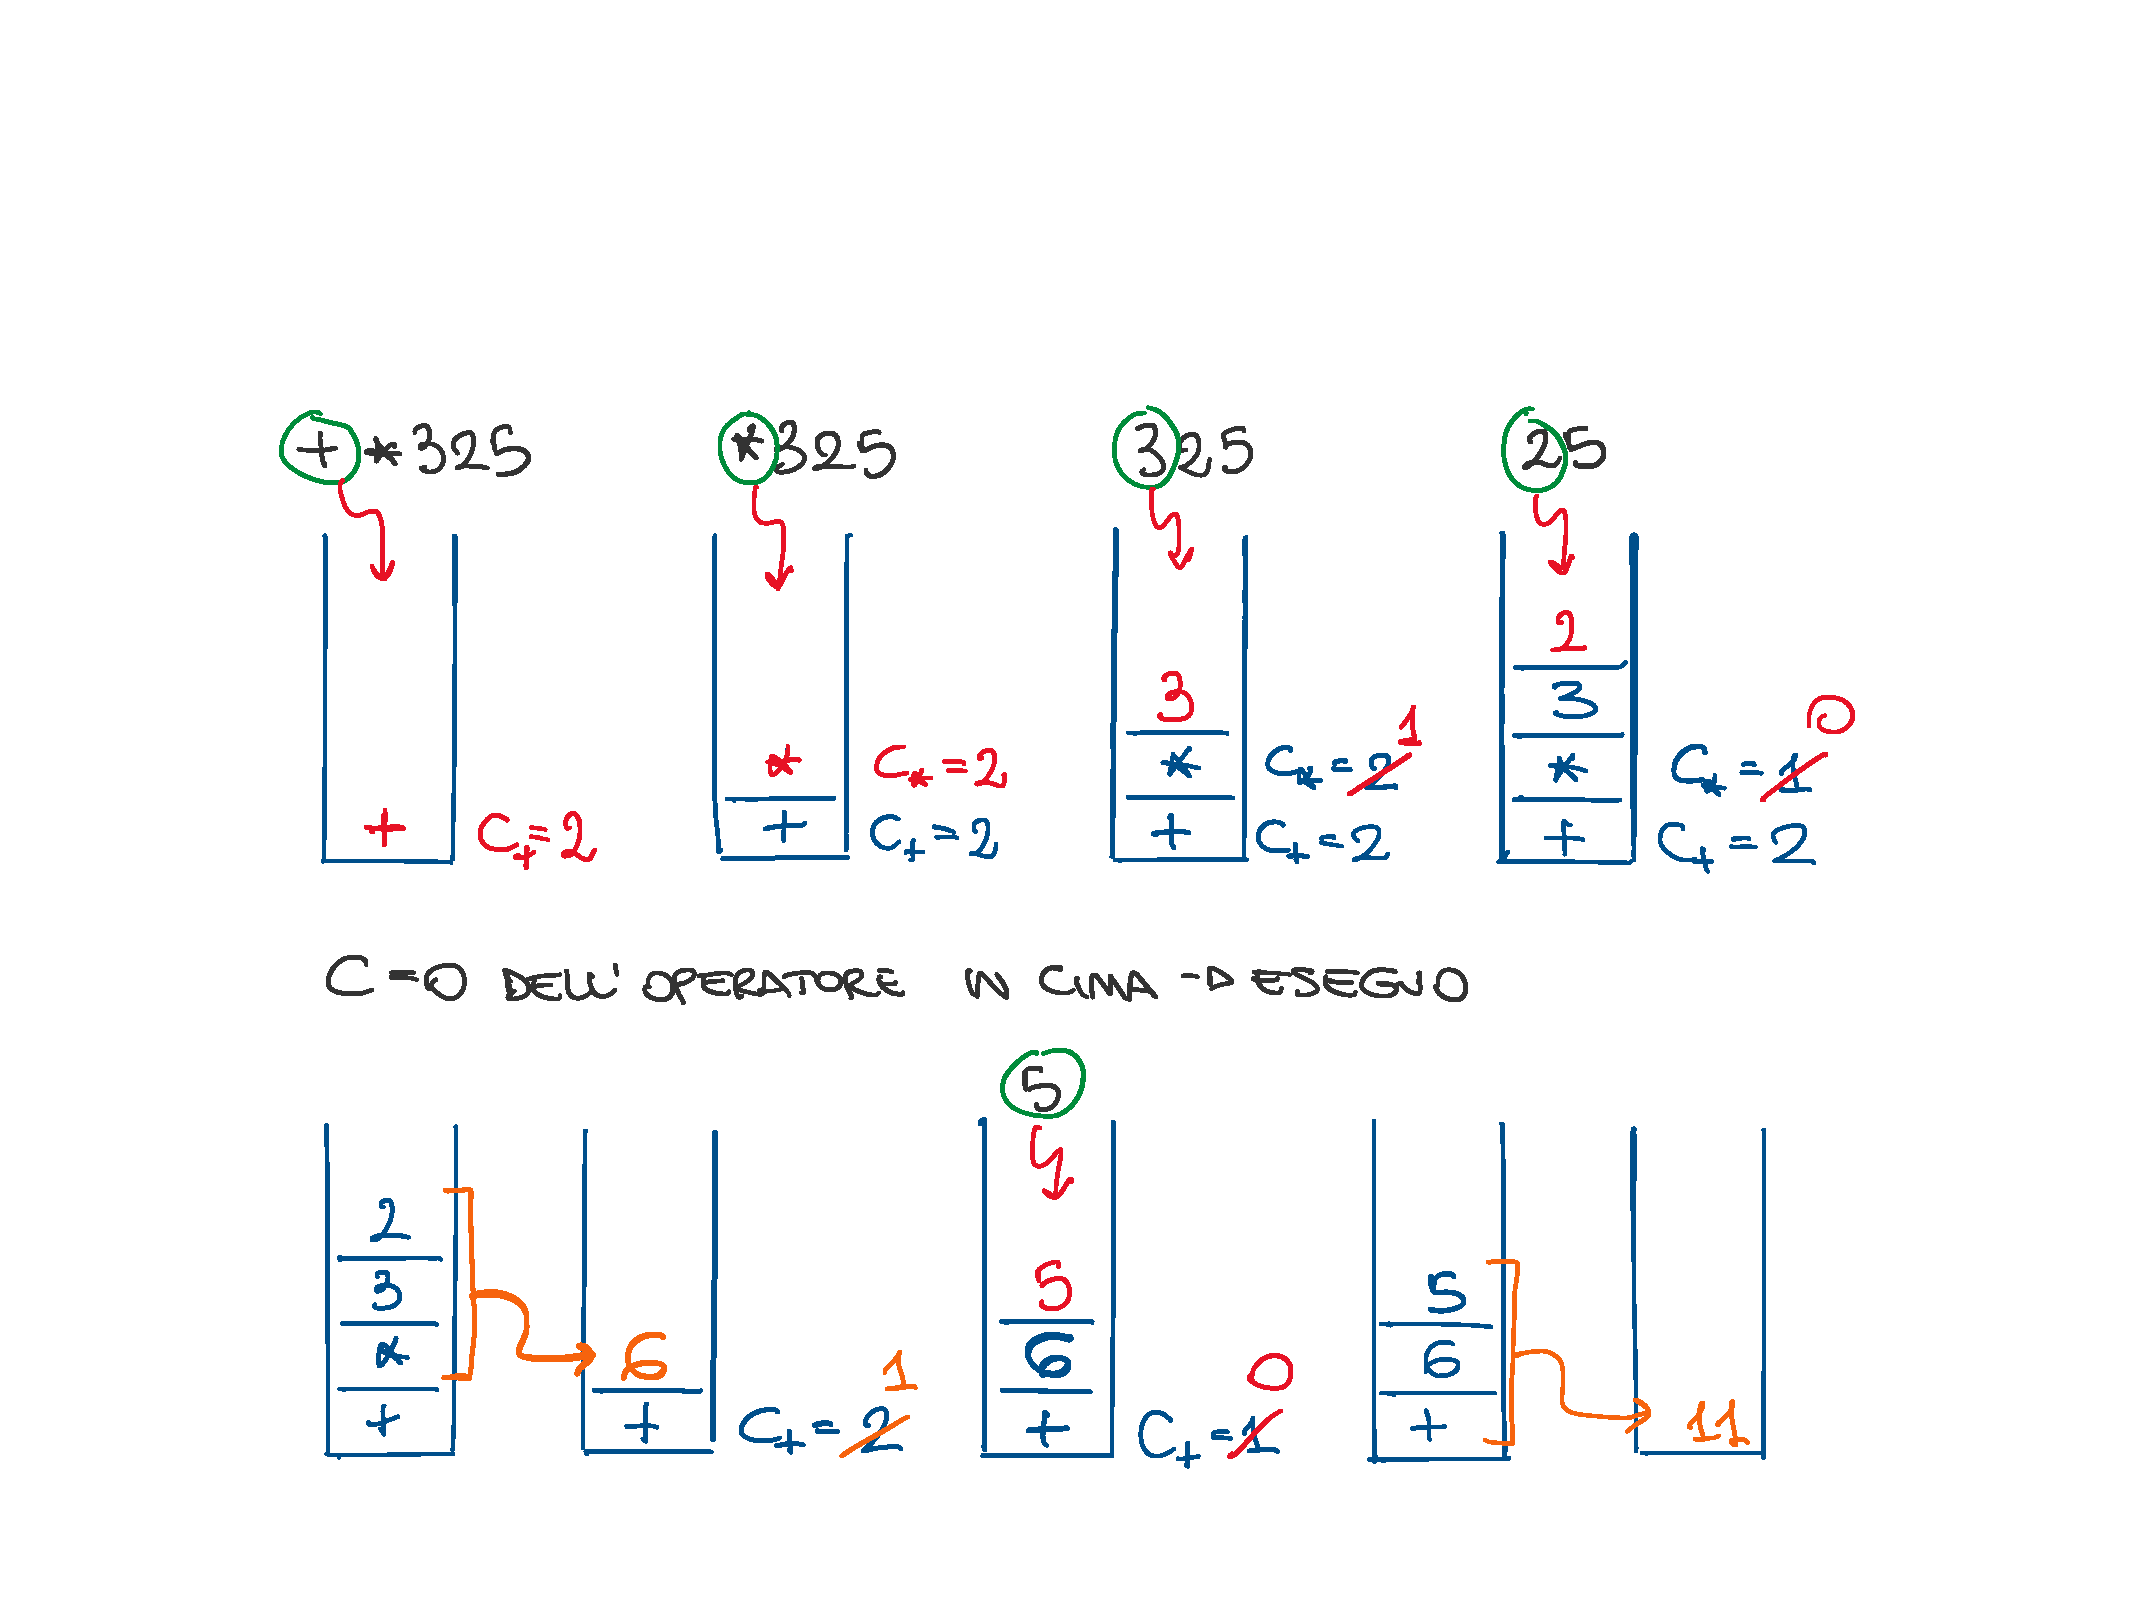
\includegraphics[width=\textwidth]{img/esempio_notazione_pre-fissa.pdf}
		\caption{Esempio di applicazione dell'algoritmo di valutazione della notazione pre-fissa.}
	\end{figure}\newpage
	
	\subsubsection{Notazione in-fissa}\label{notazione in-fissa}
	
	La notazione \textcolor{Red3}{\textbf{in-fissa}} è la \textbf{notazione più utilizzata in matematica} e nei linguaggi di programmazione come zucchero sintattico. Inoltre, è quella che consente una lettura più intuitiva ma che richiede maggiori specifiche.\newline
	
	\noindent
	Per \textcolor{Green4}{\textbf{esempio}}, considerando $15-5-3$, a seconda dell'operazione che viene eseguita per prima, cambia il risultato.\newline
	
	\noindent
	L'algoritmo di valutazione della notazione in-fissa non è così semplice come i precedenti. Infatti, a causa di alcune regole, chiamate di \textbf{precedenza} e \textbf{associatività}, e alla presenza di alcune regole, non è possibile valutare l'espressione con una semplice scansione da sinistra a destra o viceversa.\newline
	
	\noindent
	\begin{boxdef}
		Con \textcolor{Red3}{\textbf{regole di precedenza}} si intende: \textbf{le regole di precedenza di un operatore per la valutazione di un'espressione, definisce l'ordine in cui operatori \dquotes{adiacenti} a diversi livelli di precedenza vengono valutati}.
	\end{boxdef}

	\noindent
	Anche se ogni linguaggio differisce per le priorità assegnate agli operatori, l'importante è che vengano stabilite a priori. Per \textcolor{Green4}{\textbf{esempio}}, un tipico livello di precedenza è dato da: (1) parentesi, (2) operatori unari, (3) elevazione a potenza, (4) moltiplicazione e divisione, (5) somma e sottrazione.\newline
	
	\noindent
	\begin{boxdef}
		Con \textcolor{Red3}{\textbf{regole di associatività}} si intende: \textbf{le regole di associatività per la valutazione delle espressioni definiscono l'ordine con cui operatori allo stesso livello di precedenza vengono valutati}.
	\end{boxdef}

	\noindent
	Per \textcolor{Green4}{\textbf{esempio}}, delle tipiche regole di associatività sono: da sinistra verso destra; a volte operatori unitari associano da destra; in alcuni linguaggi tutti gli operatori hanno lo stesso livello di precedenza e associano da destra; le regole di precedenza e associatività possono essere sovrascritte usando le parentesi.\newline
	Un altro \textcolor{Green4}{\textbf{esempio}} $a+b-c+d$ restituisce valori diversi a seconda che si associ da destra o da sinistra.\newpage
	
	\subsection{Valutazione delle espressioni}\label{valutazione delle espressioni}
	
	La rappresentazione interna della espressioni consiste in una \textbf{rappresentazione ad albero} (\emph{abstract syntax tree}), dove i \textbf{nodi interni} sono \textbf{operatori} mentre le foglie sono valori (operandi elementari). Ogni nodo interno ha come figli gli alberi che rappresentano le espressioni a cui l'operatore si applica.\newline
	
	\noindent
	In altre parole, l'\textbf{albero fornisce la struttura dell'espressione}, ovvero:
	\begin{itemize}
		\item \textcolor{Green4}{\textbf{Aspetto positivo:}} elimina eventuali ambiguità legate a precedenze e associatività;
		\item \textcolor{Red3}{\textbf{Aspetto negativo:}} non dà informazioni riguardanti l'ordine di valutazione dell'espressione.
	\end{itemize}
	
	\noindent
	A causa delle eventuali ambiguità sulle espressioni, nasce il \textcolor{Red3}{\textbf{problema dell'ordine di valutazione}}, il quale è prettamente informatico. Infatti, la presenza di alcune caratteristiche influenzano il risultato:
	\begin{itemize}
		\item \textbf{Operandi non definiti}. Se esistono degli \textbf{operandi non definiti}, può accadere che l'espressione venga valutata solo con un preciso ordine. Per esempio, con l'espressione $\left(a == 0 ? b : b/a\right)$, è chiaro che $b/a$ può essere una divisione per $0$, quindi non definita. Tuttavia è necessario che venga valutata solo per divisioni diverse da zero, quindi un linguaggio di programmazione può essere:
		\begin{itemize}
			\item \textbf{Valutazione \textcolor{Red3}{\emph{lazy}}} (o corto circuito), ovvero gli operandi vengono valutati solo quando è necessario, quindi quando l'espressione è sempre definita.
			
			\item \textbf{Valutazione \textcolor{Red3}{\emph{eager}}}, ovvero gli operandi vengono valutati sempre.
		\end{itemize}
		Un ottimo \textcolor{Green4}{\textbf{esempio}} per comprendere la distinzione: \href{https://www.tutorialspoint.com/functional_programming_with_java/functional_programming_with_java_evaluation.htm}{link}
		
		\item \textbf{Effetti collaterali} (\emph{side effects}). Sono \textbf{effetti non legati all'oggetto di cui vi è la manipolazione}, per esempio: la valutazione di un'espressione provoca un cambiamento della memoria; una funzione modifica i propri parametri o modifica variabili non locali. Un \textcolor{Green4}{\textbf{esempio}} più tangibile è $\left(\left(a+f\left(b\right)\right) * \left(c+f\left(b\right)\right)\right)$ con la funzione $f\left(b\right)$ definita come $b++$ e l'espressione ritorna valori diversi a seconda dell'ordine di valutazione.
		
		\item \textbf{Aritmetica finita}. Nelle macchine l'\textbf{aritmetica è limitata dall'architettura, quindi i numeri non sono infiniti ed esiste un massimo numero rappresentabile}. I \textbf{problema di valutazione} avviene quando le espressioni coinvolgono tale numero.\newline
		Per \textcolor{Green4}{\textbf{esempio}} se viene eseguita una somma prima di una differenza, è possibile cambiare il risultato se la somma calcola un numero maggiore del massimo numero rappresentabile.
	\end{itemize}\newpage
	
	\subsection{Semantica delle espressioni}
	
	La \textcolor{Red3}{\textbf{semantica delle espressioni}} di un linguaggio imperativo $IMP$ cerca di descrivere la semantica senza interessarsi della grammatica, la quale include tutte le regole di associatività e precedenza. Quindi, vengono ignorante anche le parentesi, nonostante tutte queste regole rendono un'espressione chiara e non ambigua.\newline
	
	\noindent
	L'aspetto d'interesse è la \textbf{struttura induttiva} e non la struttura sintattica. Per questo motivo si introducono alcune definizione teoriche:
	\begin{boxdef}
		Le \textcolor{Red3}{\textbf{espressioni}} $\mathcal{E}$ è un \textbf{insieme di (alberi di valutazione) di espressioni valutate ad intero o booleano}. Gli elementi solitamente vengono rappresentati con la lettera $e$.
	\end{boxdef}
	\begin{boxdef}
		I \textcolor{Red3}{\textbf{numeri}} $\mathcal{N}$ è un \textbf{insieme di numeri reali nella macchina}. Gli elementi solitamente vengono rappresentati con le lettere $m$, $n$ o $p$.
	\end{boxdef}
	\begin{boxdef}
		I \textcolor{Red3}{\textbf{booleani}} $\mathcal{B}$ è un \textbf{insieme di valori booleani}. Composto solo da \textsf{true} e \textsf{false}. Gli elementi solitamente vengono rappresentati con la lettera $t$.
	\end{boxdef}
	
	\noindent
	Questi insiemi vengono usati per definire il \textcolor{Red3}{\textbf{sistema di transizione}}:
	\begin{equation*}
		\Gamma = \mathcal{E}, \hspace{2em} T = \mathcal{N} \cup \mathcal{B}, \hspace{2em} \mathrm{op}\in\left\{+,-,*,=\right\} \hspace{1em} \mathrm{bop} \in \left\{=, or\right\}
	\end{equation*}
	\begin{itemize}
		\item $\Gamma$ rappresenta l'insieme delle configurazioni;
		\item $\mathcal{E}$ rappresenta l'insieme delle espressioni da valutare;
		\item $T$ rappresenta l'insieme delle configurazioni terminali;
		\item $\mathrm{op}$ rappresenta l'insieme delle operazioni ammesse;
		\item $\mathrm{bop}$ rappresenta una metavariabile.
	\end{itemize}
	Quindi, viene definito l'insieme delle configurazioni come l'insieme delle espressioni da valutare $\left(\Gamma = \mathcal{E}\right)$; l'insieme delle configurazioni terminali sono un tutti i valori numerici e booleani $\left(T = \mathcal{N} \cup \mathcal{B}\right)$.\newpage
	
	\subsection{Regole di transizione}\label{regole di transizione}
	
	Si espongono qua di seguito le \textcolor{Red3}{\textbf{regole di transizione}}. Si tenga conto che con \textbf{bop} in grassetto si identifica il simbolo sintattico di un'operazione e con bop normale si identifica il simbolo dell'operazione nella macchina sottostante.\newline
	
	\noindent
	Si introducono le prime tre \textbf{regole necessarie per \underline{valutare espressioni aritmetiche}}:
	\begin{itemize}
		\item È un \underline{assioma} e \textbf{valuta l'espressione sintattica contenente un operatore aritmetico nel valore che esso rappresenta}. Per esempio, l'espressione $3+5$ viene valutata letteralmente come il valore $3$, l'operazione di somma $+$ e il valore $5$.
		\begin{gather*}
			\mathcal{E}_{1}: \:\: \mathrm{m} \:\: \textcolor{Red3}{\mathbf{op}} \:\: \mathrm{n} \rightarrow \mathrm{p} \hspace{1em} \mathrm{se} \hspace{1em} \mathrm{m} \:\: \mathrm{op} \:\: \mathrm{n} = \mathrm{p}, \\
			\mathrm{m,n,p} \in \mathcal{N}
		\end{gather*}
		
		\item È una \underline{regola induttiva} e indica che \textbf{se gli operandi non sono valori primitivi allora è necessario valutarli}.
		\begin{equation*}
			\mathcal{E}_{2}: \dfrac{
			\mathrm{e} \rightarrow \mathrm{e}'
			}{
			\mathrm{e} \:\: \textcolor{Red3}{\mathbf{op}} \:\: \mathrm{e}_{0} \rightarrow \mathrm{e}' \:\: \textcolor{Red3}{\mathbf{op}} \:\: \mathrm{e}_{0}
			}
		\end{equation*}
		
		\item La regola stabilisce che \textbf{nel momento in cui l'operando a sinistra è un valore allora è possibile iniziare a valutare l'operando a destra}. Ovviamente se anche l'operatore a destra è un valore allora si ricade nella prima regola ed è possibile restituire il valore finale.
		\begin{equation*}
			\mathcal{E}_{3} : \dfrac{
				\mathrm{e} \rightarrow \mathrm{e}'
			}{
				\mathrm{m} \:\: \textcolor{Red3}{\mathbf{op}} \:\: \mathrm{e} \rightarrow \mathrm{m} \:\: \textcolor{Red3}{\mathbf{op}} \:\: \mathrm{e}'
			}
		\end{equation*}
	\end{itemize}\newpage
	
	\begin{figure}[!htp]
		\centering
		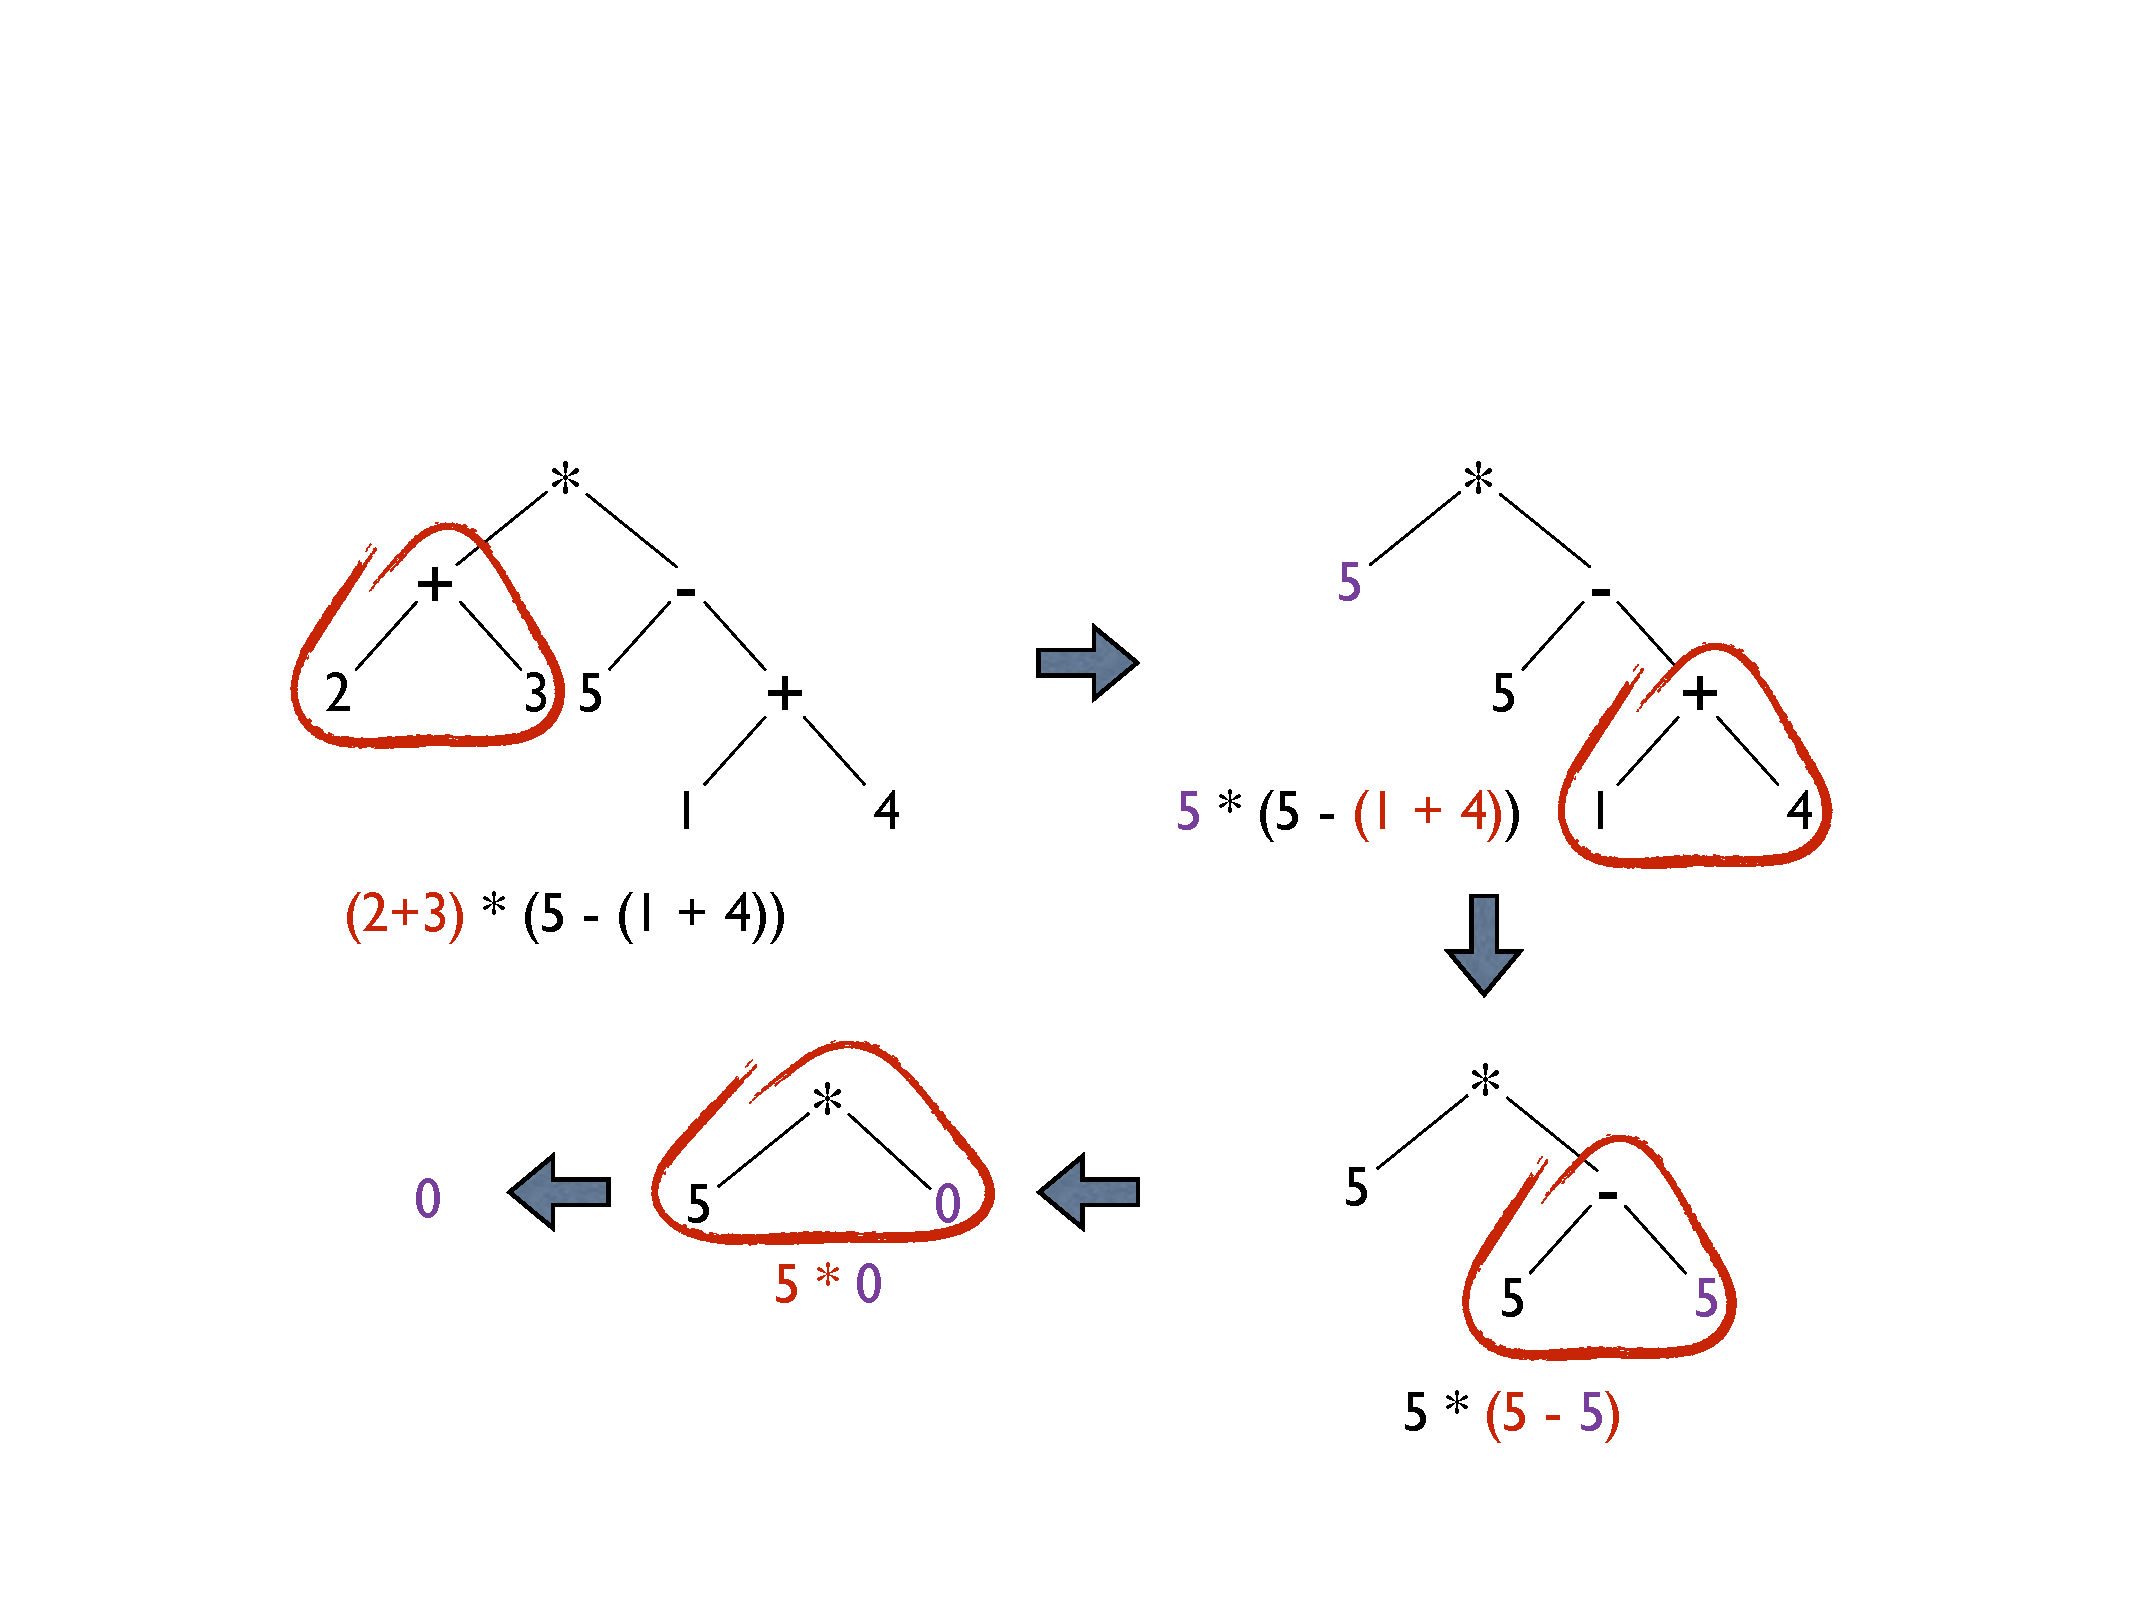
\includegraphics[width=\textwidth]{img/esempio_regole_aritmetiche.pdf}
		\caption{Esempio di applicazione delle regole aritmetiche.}
	\end{figure}
	
	\noindent
	\underline{\textbf{Attenzione!}} Non è possibile eseguire una derivazione di questo tipo:
	\begin{figure}[!htp]
		\centering
		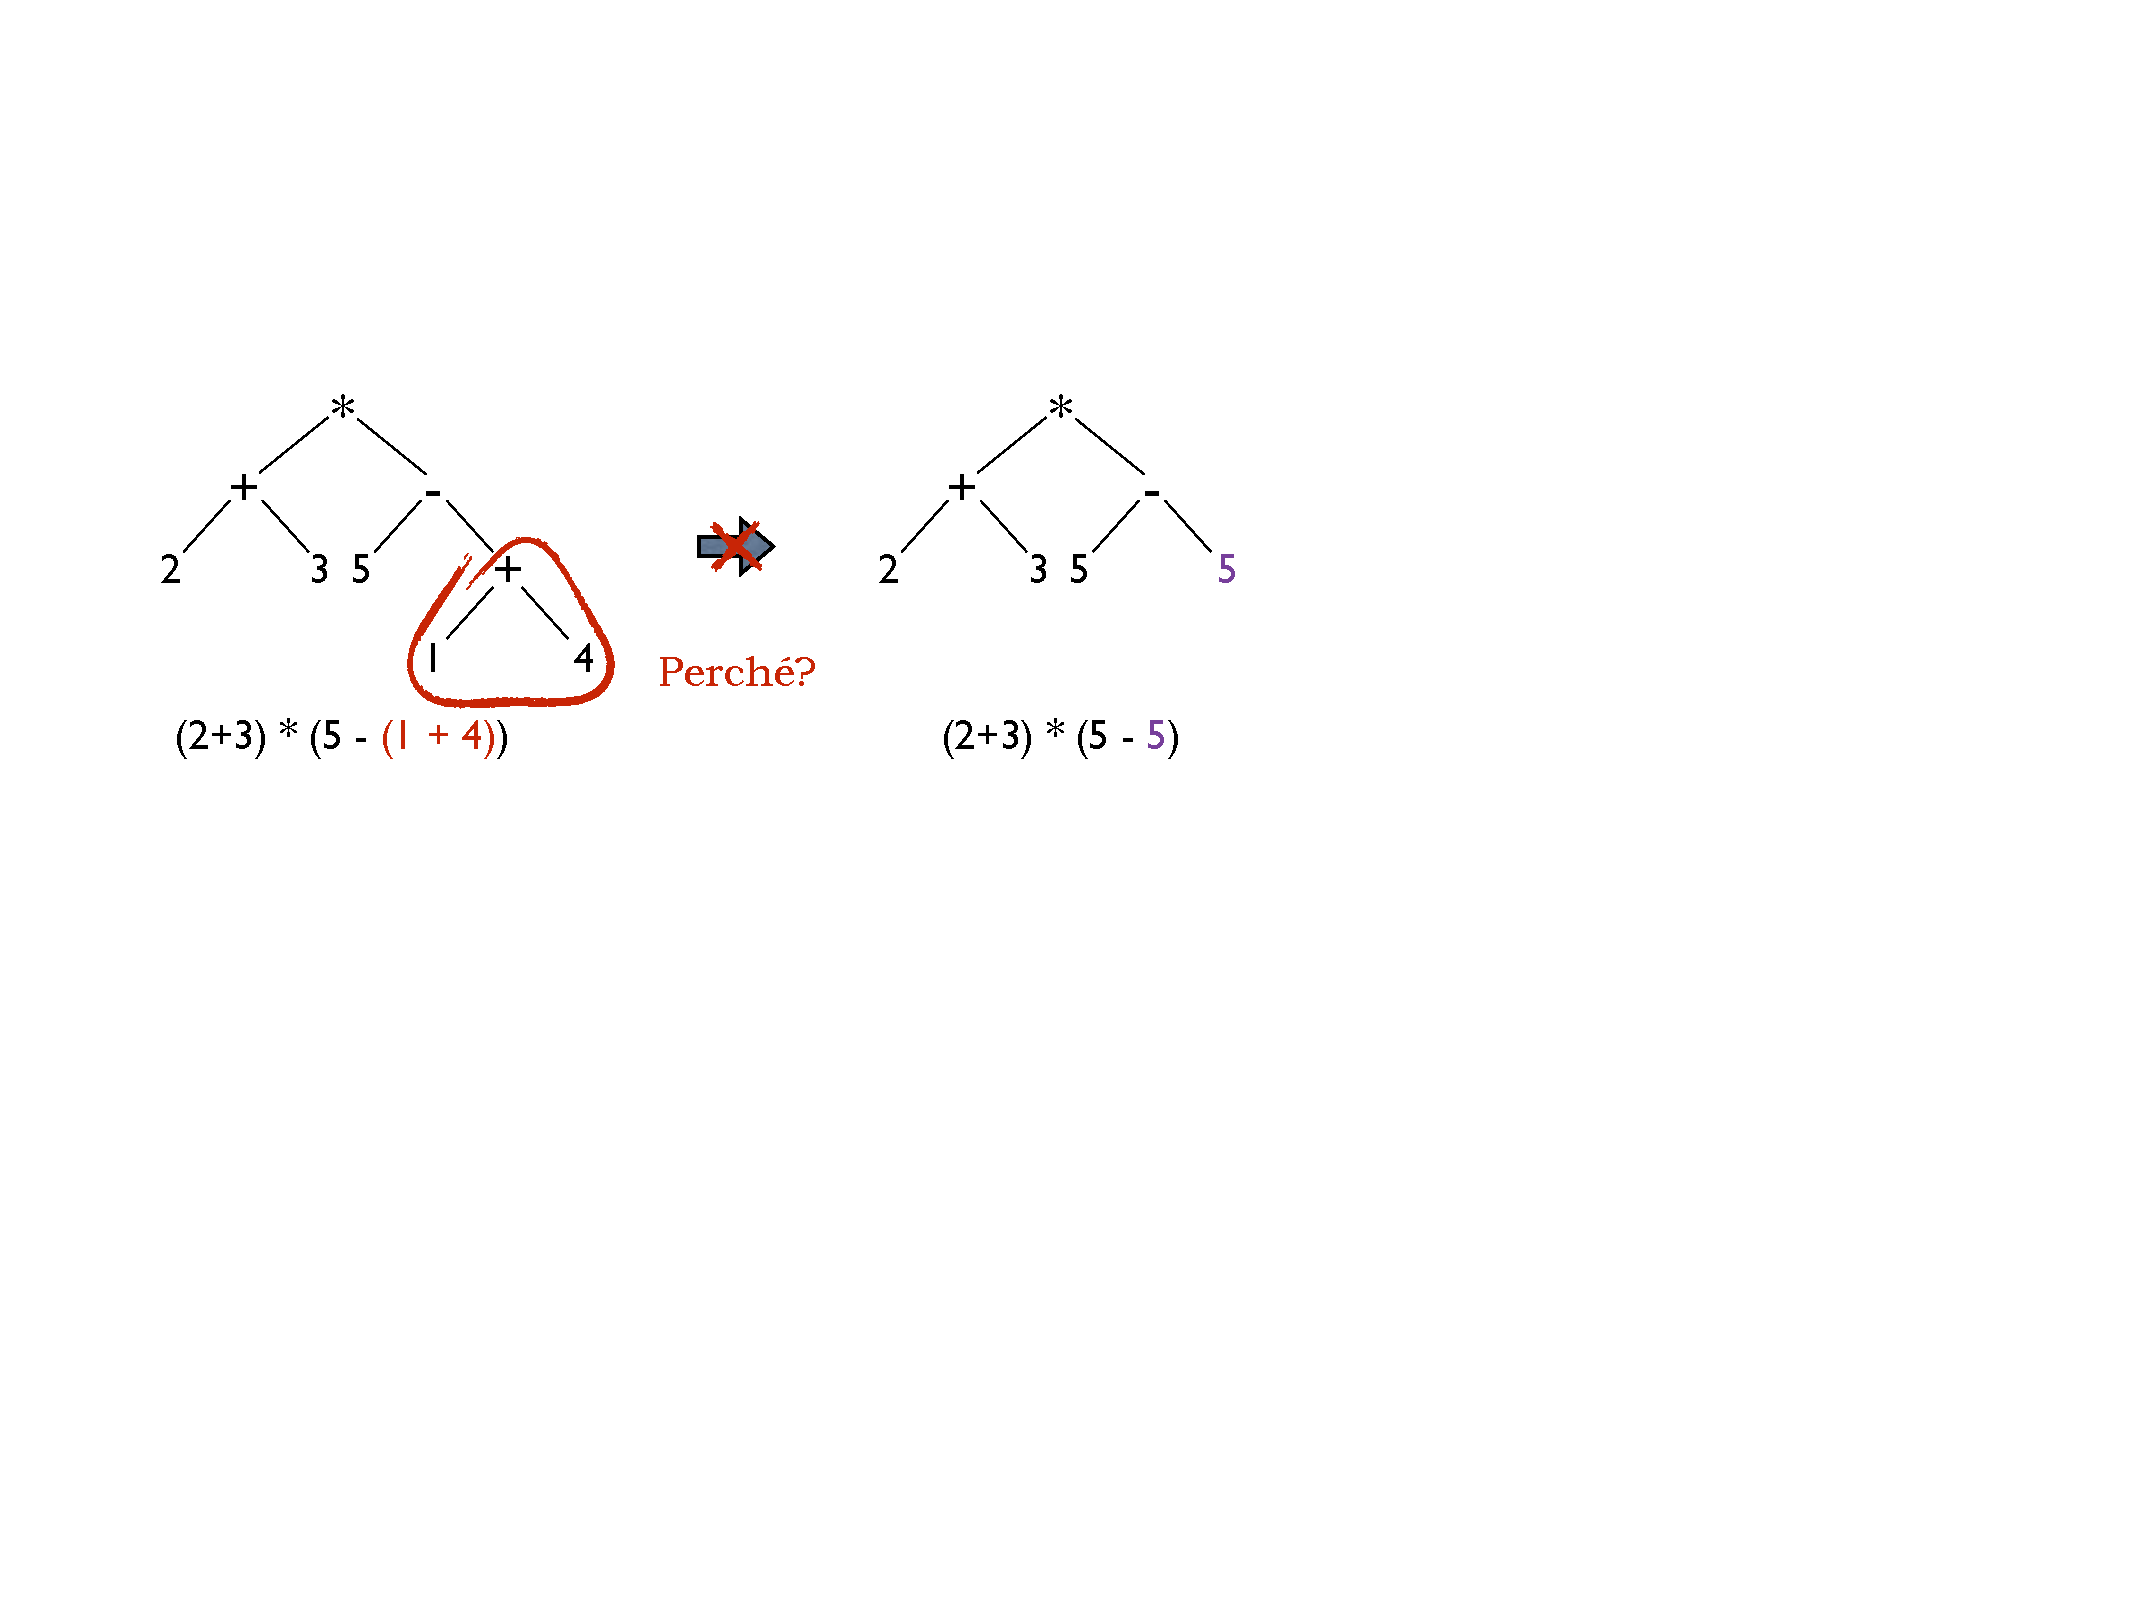
\includegraphics[width=\textwidth]{img/esempio_regole_errato.pdf}
	\end{figure}
	
	\noindent
	Questo perché le regole impongono la valutazione da sinistra verso destra e nella figura viene eseguita una valutazione da destra verso sinistra. Nonostante sia possibile implementare una nuova regola, non avrebbe senso poiché aumenterebbe la possibilità di errore nell'implementazione.
	
	\newpage
	
	\noindent
	Si continua con le regole necessarie per valutare le espressioni booleane (ricordando che \textbf{bop} è il simbolo sintattico di un'operazione e bop è il simbolo dell'operazione nella macchina sottostante):
	\begin{itemize}
		\item È un \underline{assioma} che \textbf{valuta l'espressione sintattica contenente un operatore, nel valore che esso rappresenta}. Ovviamente con valori booleani, i valori coinvolti devono essere tali.
		\begin{gather*}
			\mathcal{E}_{4} : \:\: \mathrm{k}_{1} \:\: \textcolor{Red3}{\mathbf{bop}} \:\: \mathrm{k}_{2} \rightarrow \mathrm{t} \hspace{1em} \mathrm{se} \hspace{1em} \mathrm{k}_{1} \:\: \mathrm{bop} \:\: \mathrm{k}_{2} = \mathrm{t}, \\
			\mathrm{k_{1}, k_{2}} \in \mathcal{B} \cup \mathcal{N}, \hspace{1em} \mathrm{t} \in \mathcal{B}, \hspace{1em} \textcolor{Red3}{\mathbf{bop}} \in \left\{=, \mathrm{or}\right\}
		\end{gather*}
		
		\item Questa regola è una modifica alla precedente poiché \textbf{ammette che l'espressione contenga operatori binari booleani}. L'ordine di valutazione è da sinistra verso destra.
		\begin{equation*}
			\mathcal{E}_{3'} : \dfrac{
				\mathrm{e} \rightarrow \mathrm{e}'
			}{
				\mathrm{e} \:\: \textcolor{Red3}{\mathbf{bop}} \:\: \mathrm{e}_{0} \rightarrow \mathrm{e}' \:\: \textcolor{Red3}{\mathbf{bop}} \:\: \mathrm{e}_{0}
			}
		\end{equation*}
		
		\item Questa regola stabilisce che nel momento in cui l'\textbf{operando a sinistra è un valore booleano allora è possibile iniziare a valutare l'operando a destra}. Ovviamente, se l'operatore a destra è un valore booleano, allora si ricade nell'assioma $\mathcal{E}_{4}$ ed è possibile restituire il valore finale.
		\begin{equation*}
			\mathcal{E}_{5} : \dfrac{
				\mathrm{e} \rightarrow \mathrm{e}'
			}{
				\mathrm{t} \:\: \textcolor{Red3}{\mathbf{op}} \:\: \mathrm{e} \rightarrow \mathrm{t} \:\: \textcolor{Red3}{\mathbf{op}} \:\: \mathrm{e}'
			}
		\end{equation*}
		
		\item Nel caso booleano è necessario aggiungere la \textbf{regola per l'operatore unario}. Quindi si crea l'\underline{assioma} che \textbf{restituisce il valore corrispondente all'applicazione dell'operatore sul valore rappresentato}.
		\begin{equation*}
			\mathcal{E}_{6} : \:\: \textcolor{Red3}{\mathbf{not}} \:\: \mathrm{t}_{1} \rightarrow \mathrm{t} \hspace{1em} \mathrm{se} \hspace{1em} \mathrm{not} \:\: \mathrm{t}_{1} = \mathrm{t}, \mathrm{t}_{1} \in \mathcal{B}
		\end{equation*}
		
		\item Sempre nel caso booleano, si deve creare la \textbf{regola di valutazione}, analoga alle precedenti.
		\begin{equation*}
			\mathcal{E}_{7} : \dfrac{
				\mathrm{e} \rightarrow \mathrm{e}'
			}{
				\textcolor{Red3}{\mathbf{not}} \:\: \mathrm{e} \rightarrow \textcolor{Red3}{\mathbf{not}} \:\: \mathrm{e}'
			}
		\end{equation*}
	\end{itemize}\newpage
	
	\subsection{Valutazione ed equivalenza}
	
	\begin{boxdef}
		La \textcolor{Red3}{\textbf{valutazione delle espressioni}} è una \textbf{funzione $Eval: \mathcal{E} \rightarrow \mathbb{N} \cup \mathbb{B}$ che descrive il comportamento dinamico delle espressioni restituendo il valore in cui esse sono valute}:
		\begin{equation*}
			Eval\left(e\right) = k \iff e \rightarrow^* k
		\end{equation*}
	\end{boxdef}\:\newline

	\begin{boxdef}
		L'\textcolor{Red3}{\textbf{equivalenza di espressioni}} è una \textbf{relazione $\equiv \subseteq \mathcal{E} \times \mathcal{E}$ definita come segue}:
		\begin{equation*}
			e_{0} \equiv e_{1} \iff Eval\left(e_{0}\right) = Eval\left(e_{1}\right)
		\end{equation*}
	\end{boxdef}\newpage

	\section{Dichiarazioni}
	
	\subsection{Identificatori}
	
	Gli \textbf{identificatori} sono \textbf{sequenze di caratteri}, che hanno lo \textbf{scopo di denotare} (identificatore appunto) \textbf{qualcos'altro}.\newline
	
	\noindent
	In altre parole, gli \textbf{identificatori sono nomi usati per riferire altri elementi del linguaggio}, come le procedure, \textbf{o della macchina sottostante}, come le colle di memoria, \textbf{durante la computazione}, senza necessariamente conoscerne il valore a priori.\newline
	
	\noindent
	Gli \textbf{identificatori} sono detti \textbf{variabili} quando identificano celle di memoria.\newline
	
	\noindent
	I \textbf{nomi} sono fondamentali per gli identificatori perché sono \textbf{facili da ricordare} e consentono di effettuare un processo di \textbf{astrazione}. Inoltre, è importante sottolineare il fatto che un identificatore ed un oggetto denotato \underline{non} sono la stessa cosa:
	\begin{itemize}
		\item Un identificatore può denotare più elementi;
		\item Un elemento può essere denotato da più identificatori diversi (\emph{aliasing})
	\end{itemize}
	Un \textcolor{Green4}{\textbf{esempio}} è il seguente codice:
	\begin{lstlisting}[language=C]
const pi = 3.14;
int x;
void f(){...};\end{lstlisting}
	Gli oggetti denotati sono una costante, una variabile e una procedura:
	\begin{itemize}
		\item \textsf{3.14} è una costante;
		\item \textsf{x} è una variabile;
		\item \textsf{\{...\}} è una procedura
	\end{itemize}
	Mentre \textsf{pi, x, f} sono nomi.\newline
	
	\noindent
	In definitiva, gli identificatori non possono essere stringhe di caratteri qualunque, ma devono seguire delle regole così che il \emph{parser} del linguaggio li possa riconoscere come tali.\newline
	
	\noindent
	\begin{boxdef}
		Gli \textcolor{Red3}{\textbf{identificatori}} sono una \textbf{sequenza di caratteri usata per rappresentare o \underline{denotare} un altro oggetto}.
	\end{boxdef}\newpage
	
	\subsection{Bindings}
	
	\subsubsection{Legami}
	
	\begin{boxdef}
		Il \textcolor{Red3}{\textbf{\emph{binding occurrences}}} o in italiano la \textcolor{Red3}{\textbf{creazione \emph{binding}}} è il momento in cui viene \textbf{\underline{definito} il nome (identificatore) e il suo significato (denotazione)}.
	\end{boxdef}

	\noindent
	In \textbf{matematica} questo accade ogni volta che viene posto un problema enunciando (e.g.) \dquotes{sia $x$ ...}. Viene creato un \emph{binding} \textbf{tra il significato dichiarato e il nome che verrà poi utilizzato nella specifica del problema}. In \textbf{logica} i \emph{binding} sono creati dai quantificatori (universali o esistenziali).\newline
	
	\noindent
	In \textbf{programmazione} i \emph{binding} sono creati dalle dichiarazioni. Successivamente, il nome può essere correttamente utilizzato per riferirsi/rappresentare il suo significato.\newline
	
	\noindent
	\begin{boxdef}
		L'\textcolor{Red3}{\textbf{\emph{applied occurrences}}} o in italiano l'\textcolor{Red3}{\textbf{applicazione \emph{binding}}} è il momento in cui viene \textbf{\underline{utilizzato} il nome (identificatore) per \underline{accedere} al suo significato (denotazione)}.
	\end{boxdef}

	\noindent
	In programmazione, come in matematica, non è sempre necessario creare i \emph{binding} prima del loro utilizzo, dipende dal linguaggio di programmazione.\newline
	
	\noindent
	Un \textcolor{Green4}{\textbf{esempio}} di creazione e applicazione:
	\begin{gather*}
		\displaystyle\sum_{i=1}^{n}\sum_{j=1}^{m}a_{ij} \cdots b_{jk} \\
		\downarrow \\
		\displaystyle\underbrace{\sum_{i=1}^{n}\sum_{j=1}^{m}}_{\text{\emph{Binding occurrences i,j}}} \overbrace{a_{ij} \cdots b_{jk}}^{\text{\emph{Applied occurrences i,j}}}
	\end{gather*}
	La $i$ e $j$ sotto il simbolo di sommatoria sulla sinistra indicano la creazione del \emph{binding} e la $i,j$ a pedice dei simboli $a$ e $b$ sulla destra indicano l'applicazione del \emph{binding}.\newpage
	
	\subsubsection{Scope}
	
	Esistono anche le occorrenze libere che sono simili a quelle applicate con l'unica differenza che riguarda il raggio di azione (\emph{scope}) di un'occorrenza di definizione.\newline
	
	\noindent
	\begin{boxdef}
		Le \textcolor{Red3}{\textbf{\emph{free occurrences}}} o in italiano le \textcolor{Red3}{\textbf{occorrenze libere}} (non legate) è il momento in cui viene \textbf{\underline{utilizzato} un nome (identificatore) il cui significato (denotazione) non è stato definito}.
	\end{boxdef}\:\newline

	\noindent
	\begin{boxdef}
		Lo \textcolor{Red3}{\textbf{\emph{scope} di un \emph{binding}}} o in italiano il \textcolor{Red3}{\textbf{raggio d'azione di una definizione}} è la \textbf{definizione di spazio in cui è possibile utilizzare un nome per rappresentare il significato associato da un \emph{binding}}.
	\end{boxdef}\:\newline

	\noindent
	Un \textcolor{Green4}{\textbf{esempio}} di creazione e applicazione:
	\begin{gather*}
		\displaystyle\sum_{i=1}^{n}\sum_{j=1}^{m}a_{ij} \cdots b_{jk} \\
		\downarrow \\
		\displaystyle\underbrace{\sum_{i=1}^{n}\overbrace{\sum_{j=1}^{m} a_{ij} \cdots b_{jk}}^{\text{Scope di \emph{j}}}}_{\text{Scope di \emph{i}}}
	\end{gather*}
	La $n$, la $m$ e la $k$ sopra il simbolo di sommatoria sulla sinistra e al pedice della $b$, indicano le occorrenze libere, cioè non legate. Invece, lo \emph{scope} di $j$ si concentra sulla sommatoria più innestata, mentre lo \emph{scope} di $i$ sulla sommatoria più esterna.\newpage
	
	
	\subsubsection{Bindings nei linguaggi di programmazione}
	
	Si riportano le definizioni già date ma con una veste diversa (non so il motivo di questa scelta, ma sulle slide è così...).\newline
	
	\noindent
	\begin{boxdef}
		\textcolor{Red3}{\textbf{Definizione - \emph{Binding occurrence}:}} un identificatore in posizione di definizione quando si \emph{(ri)definisce il significato} dell'identificatore.
	\end{boxdef}\:\newline

	\noindent
	\begin{boxdef}
		\textcolor{Red3}{\textbf{Uso - \emph{Applied occurrence}:}} un identificatore in posizione di uso quando si \emph{riferisce/denota il significato} definito da una definizione.
	\end{boxdef}\:\newline
	
	\noindent
	\begin{boxdef}
		\textcolor{Red3}{\textbf{Libera - \emph{Free occurrence}:}} un identificatore in posizione libera se il suo uso non è nel \emph{raggio di azione (scope)} di una definizione.
	\end{boxdef}\newpage
	
	
	\subsubsection{Tipi di bindings nei linguaggi di programmazione}
	
	A seconda dell'oggetto denotato, il \emph{binding} creato è di tipo diverso:
	\begin{itemize}
		\item \textbf{Nome-Valore}: quando il \textbf{legame non può cambiare}, allora viene legato il nome ad un valore.
		
		\item \textbf{Nome-Locazione}: \textbf{legame non modificabile}
		
		\item \textbf{Locazione-Valore} \textbf{legame modificabile}
	\end{itemize}
	Tutti i \textbf{legami} sono \textbf{immutabili} ed esistono due tipi di \emph{binding}:
	\begin{itemize}
		\item \textbf{Binding \emph{statico}} è tale \textbf{se occorre per la prima volta prima dell'esecuzione e rimane invariato durante tutta l'esecuzione del programma}.\newline
		Per \textcolor{Green4}{\textbf{esempio}}, i tipi delle variabili in linguaggi fortemente tipati.
		
		\item \textbf{Binding \emph{dinamico}} è tale \textbf{se occorre durante l'esecuzione e può variare}.\newline
		Per \textcolor{Green4}{\textbf{esempio}}, i \textbf{legami tra locazioni/celle di memoria e valori contenuti nelle locazioni}.
	\end{itemize}\newpage
	
	\subsubsection{Tempi}
	
	Esistono due \textbf{tipi di \underline{creazione} dei \emph{binding}}:
	\begin{itemize}
		\item \textcolor{Red3}{\textbf{Tempo di compilazione}} (\emph{Early binding}). Ogni nome viene risolto a tempo di compilazione, quindi è presente un'\textbf{allocazione statica della memoria} con indirizzi assoluti.
		\begin{itemize}
			\item \textcolor{Green4}{\textbf{Pro:}} esecuzione estremamente veloce
			
			\item \textcolor{Red3}{\textbf{Contro:}} programmazione poco flessibile
			
			\item \textbf{Esempi di linguaggi:}  Fortran\footnote{Un interessante articolo sul perché Fortran viene ancora utilizzato: \href{https://www.matecdev.com/posts/why-fortran-still-used.html}{link}}, Cobol.
		\end{itemize}
		
		\item \textcolor{Red3}{\textbf{Tempo di esecuzione}} (\emph{Late binding}). Tutto avviene a tempo di esecuzione, quindi la \textbf{memoria è allocata dinamicamente}, tutti i \emph{binding} vengono creati dinamicamente con indirizzi non assoluti.
		\begin{itemize}
			\item \textcolor{Green4}{\textbf{Pro:}} programmazione più flessibile
			
			\item \textcolor{Red3}{\textbf{Contro:}} esecuzione più lenta
			
			\item \textbf{Esempi di linguaggi:} Snobol4, Lisp, APL.
		\end{itemize}
	\end{itemize}
	Invece, qui di seguito vengono elencati degli \textbf{esempi di tempi di bindings}:
	\begin{itemize}
		\item Tempo di \textbf{progettazione}, \emph{bindings} di operatori ($+,-,...$) ai simboli;
		
		\item Tempo di \textbf{implementazione di linguaggi}, \emph{binding} del tipo floating point con la propria rappresentazione;
		
		\item Tempo di \textbf{compilazione}, \emph{binding} delle variabili con i loro tipo, come in C o Java;
		
		\item Tempo di \textbf{caricamento}, \emph{binding} variabili \textsf{static} alla cella di memoria;
		
		\item Tempo di \textbf{esecuzione}, \emph{binding} variabili non statiche con la cella di memoria.
	\end{itemize}
	Quindi, dovrebbe essere chiara la \textbf{fondamentale importanza dei \emph{bindings}}: un identificatore/nome non ha significato se non è legato a qualcosa, se non è coinvolto almeno in un \emph{binding}. Per \textcolor{Green4}{\textbf{esempio}}, un'espressione non ha significato/valore se contiene nomi non legati a nulla.\newpage
	
	
	\subsection{Semantica: Identificatori, ambienti e dichiarazioni}
	
	Nei linguaggi di programmazione, per riferire \textbf{valori generati dalle espressioni}, viene utilizzato il concetto di \textcolor{Red3}{\textbf{identificatore}}. Esso è un \textbf{nome che viene associato all'oggetto da identificare/riferire}.\newline
	
	\noindent
	Per riferire i valori (oggetti denotabili) associati agli identificatori, viene utilizzato il concetto di \textcolor{Red3}{\textbf{ambiente}}, il quale è definito come l'insieme di legami (\emph{bindings}) tra identificatori e oggetti \textbf{denotabili}, ovvero tutti quegli oggetti del linguaggio che sono riferibili mediante un identificatore.
	
	In altre parole, l'ambiente è la componente della macchina astratta che per ogni nome introdotto dal programmatore, e per ogni punto di programma, consente di determinare quale sia l'associazione corretta.\newline
	
	\noindent
	Infine, la \textbf{dichiarazione} implementa la creazione dei legami.\newline
	
	\noindent
	\begin{boxdef}
		L'\textcolor{Red3}{\textbf{ambiente}} è l'\textbf{insieme delle associazioni fra nomi e oggetti denotabili esistenti a \emph{run-time} in uno specifico punto del programma ed in uno specifico momento dell'esecuzione}.
	\end{boxdef}
	\begin{boxdef}
		La \textcolor{Red3}{\textbf{dichiarazione}} è il \textbf{meccanismo (implicito o esplicito) col quale si crea un'associazione nell'ambiente}.
	\end{boxdef}\newpage

	
	\subsubsection{Termini chiusi e ground}
	
	\begin{boxdef}
		\textbf{In un linguaggio (con identificatori),un \textcolor{Red3}{termine} in cui non ci sono identificatori liberi è detto \textcolor{Red3}{chiuso}.}
	\end{boxdef}
	
	\noindent
	Il significato delle frasi chiuse è quello di \textbf{dare significato alla frase senza richiedere un ambiente esterno}. In termini tecnici, significa che un \textbf{programma}, ad esempio, \textbf{non ha identificatori liberi e quindi può essere eseguito a partire da un ambiente vuoto}, in quanto non ci sono identificatori che richiedono un significato all'esterno.\newline

	\noindent
	Per \textcolor{Green4}{\textbf{esempio}}, non è possibile dare significato ad $a+b+c+x$ se non viene dato un significato ad $a,b,c,x$. È dunque necessario di assunzioni sull'ambiente, le quali riguardano l'insieme di \emph{binding} per gli identificatori, ovvero uguaglianze del tipo $nome = entità$.\newline
	
	\noindent
	Quindi, un \textbf{programma è una \textcolor{Red3}{frase chiusa} se ogni occorrenza d'uso è preceduta da un'occorrenza di definizione che stabilisce il significato dell'identificatore}.\newline
	
	\noindent
	\begin{boxdef}
		\textbf{In un linguaggio (con identificatori), un \textcolor{Red3}{termine} in cui non ci sono identificatori è detto \textcolor{Red3}{\emph{ground}}.}
	\end{boxdef}
	
	\noindent
	Data l'assenza di identificatori, il \textbf{termine \emph{ground}} non richiede neanche un ambiente.\newpage
	
	\subsubsection{Ambienti nei linguaggi imperativi}
	
	Nel \textbf{linguaggio imperativo} si considerano solo \textbf{interi e booleani} (per semplicità), quindi gli unici oggetti denotabili sono:
	\begin{equation*}
		\begin{array}{rl}
			\mathcal{N} = \text{ Insieme di numerali nella macchina sottostante:} & \textsf{m,n,p} \\
			\mathcal{B} = \left\{\textsf{true}, \textsf{false}\right\}: & \textsf{t}
		\end{array}
	\end{equation*}
	\begin{boxdef}
		Un \textcolor{Red3}{\textbf{ambiente dinamico}} è un elemento dello spazio di funzioni tale che:
		\begin{equation*}
			Env = \cup_{V \subseteq_{f} Id} Env_{V}
		\end{equation*}
		In cui:
		\begin{equation*}
			Env_{V}: V \rightarrow DVal \hspace{2em} \cup\left\{\bot\right\} \text{ ha metavariabile }\rho
		\end{equation*}
	\end{boxdef}
	
	\noindent
	I valori denotabili, nel linguaggio imperativo scelto, costituiscono l'insieme $DVal = \left\{Int \cup Bool\right\}$.\newline\label{DVal}
	
	\noindent
	L'ambiente associa identificatori agli oggetti denotabili ($\bot$ va associato all'identificatore non definito, ovvero non associato ad alcun valore). Quindi, un \textbf{ambiente} per un insieme di identificatori finito $V\left(Env_{V}\right)$ è una \textbf{funzione che ad ogni identificatore associa un valore denotabile, oppure il valore non definito }$\bot$. L'ambiente è l'unione di tutte queste funzioni al variare dell'insieme $V$.
	
	\longline
	
	\subsubsection{Espressioni con identificatori}
	
	Le espressioni arricchite con la semantica degli identificatori è la seguente. La sintassi è la grammatica completa delle espressioni:
	\begin{equation*}
		\begin{array}{rll}
			\mathrm{<Exp>} & & \\
			\mathrm{E} & \rightarrow & \mathrm{A} \:\: | \:\: \mathrm{B} \\
			\mathrm{A} & \rightarrow & \mathrm{I} \:\: | \:\: \mathrm{n} \:\: | \:\: \mathrm{A} \: \mathrm{op} \: \mathrm{A} \\
			\mathrm{B} & \rightarrow & \mathrm{I} \:\: | \:\: \mathrm{true} \:\: | \:\: \mathrm{false} \:\: | \:\: \mathrm{not} \: \mathrm{B} \:\: | \:\: \mathrm{B} \: \mathrm{or} \: \mathrm{B} \:\: | \:\: \mathrm{A} = \mathrm{A}
		\end{array}
	\end{equation*}
	
	\noindent
	Poi si definisce l'insieme $\mathcal{E}^{V}$ delle espressioni (con identificatori) valutate ad intero o booleano. Quindi, il sistema di transizione diventa:
	\begin{equation*}
		\Gamma = \mathcal{E}^{V}, \hspace{1em} T = \mathcal{N} \cup \mathcal{B}, \hspace{1em} \mathrm{op} \in \left\{+,-,*,=\right\}, \hspace{1em} \mathrm{bop} \in \left\{=, or\right\}
	\end{equation*}
	Inoltre, le regole definite nel paragrafo \ref{regole di transizione} devono essere riscritte integrando l'ambiente. Tutte le regole $\mathcal{E}_{i}$ diventano:
	\begin{equation*}
		\mathcal{E}_{\mathrm{i}} : \:\: \textcolor{Red3}{\rho \:\: \vdash} \:\: \mathrm{e} \: \rightarrow_{\mathrm{e}} \: \mathrm{e}'
	\end{equation*}

	\noindent
	In cui $\rho$ è l'ambiente di valutazione delle espressioni, ovvero la specifica dell'associazione tra identificatori e oggetti denotati, e il pedice della freccia ($\rightarrow_{e}$) denota quale sistema di transizione si sta utilizzando.\newpage
	
	
	\subsubsection{Identificatori liberi}
	
	\begin{boxdef}
		Un identificatore è in posizione libera (\textcolor{Red3}{\textbf{occorrenza libera}}) (\textbf{\emph{free occurrence}}) se il suo uso (\emph{applied occurrence}) non è nel \textbf{raggio di azione (scope)} di una definizione.
	\end{boxdef}\newpage
	
	
	\subsection{Nuove regole}\label{nuove regole}
	
	Per una descrizione dettagliata delle regole si rimanda al paragrafo \ref{regole di transizione}:
	\begin{itemize}
		\item La prima regola:
		\begin{gather*}
			\mathcal{E}_{1} : \:\: \textcolor{Red3}{\rho \:\: \vdash} \:\: \mathrm{m} \:\: \textcolor{Red3}{\mathbf{op}} \:\: \mathrm{k} \: \rightarrow_{e} \: \mathrm{p} \\
			\mathrm{se} \hspace{1em} \mathrm{m} \:\: \mathrm{op} \:\: \mathrm{n} = \mathrm{k}, \hspace{1em} \mathrm{m,n} \in \mathcal{N}, \hspace{1em} \mathrm{k} \in \mathcal{N} \cup \mathcal{B}
		\end{gather*}
		
		\item La seconda regola cambia, in quanto ora è necessario l'assioma per gli identificatori. In questo \textbf{assioma}, quando si incontra un identificatore, questo viene valutato nel valore che l'ambiente associa all'identificatore. Ovviamente, questa regola è applicabile solo se $I$ è un identificatore per il quale $\rho$ esiste un'associazione.
		\begin{equation*}
			\mathcal{E}_{2} : \:\: \textcolor{Red3}{\rho \:\: \vdash} \:\: \mathrm{I} \: \rightarrow_{\mathrm{e}} \: \mathrm{n} \hspace{1em} \mathrm{se} \hspace{1em} \rho\left(\mathrm{I}\right) = \mathrm{n}
		\end{equation*}
		
		\item La terza regola:
		\begin{equation*}
			\mathcal{E}_{3} : \dfrac{
			\textcolor{Red3}{\rho \:\: \vdash} \:\: \mathrm{e} \: \rightarrow_{\mathrm{e}} \: \mathrm{e}'
			}{
			\textcolor{Red3}{\rho \:\: \vdash} \:\: \mathrm{e} \:\: \textcolor{Red3}{\mathrm{\mathbf{op}}} \:\: \mathrm{e}_{0} \: \rightarrow_{\mathrm{e}} \: \mathrm{e}' \:\: \textcolor{Red3}{\mathrm{\mathbf{op}}} \:\: \mathrm{e}_{0}
			}
		\end{equation*}
		
		\item La quarta regola:
		\begin{equation*}
			\mathcal{E}_{4} : \dfrac{
				\textcolor{Red3}{\rho \:\: \vdash} \:\: \mathrm{e} \: \rightarrow_{\mathrm{e}} \: \mathrm{e}'
			}{
				\textcolor{Red3}{\rho \:\: \vdash} \:\: \mathrm{m} \:\: \textcolor{Red3}{\mathrm{\mathbf{op}}} \:\: \mathrm{e} \: \rightarrow_{\mathrm{e}} \: \mathrm{m} \:\: \textcolor{Red3}{\mathrm{\mathbf{op}}} \:\: \mathrm{e}'
			}
		\end{equation*}
		
		\item La quinta regola:
		\begin{gather*}
			\mathcal{E}_{5} : \:\: \textcolor{Red3}{\rho \:\: \vdash} \:\: \mathrm{k}_{1} \:\: \textcolor{Red3}{\mathbf{bop}} \:\: \mathrm{k}_{2} \: \rightarrow_{\mathrm{e}} \: \mathrm{t} \\
			\mathrm{se} \hspace{1em} \mathrm{k}_{1} \:\: \mathrm{bop} \:\: \mathrm{k}_{2} = \mathrm{t}, \hspace{1em} \mathrm{k_{1},k_{2}} \in \mathcal{N} \cup \mathcal{B}, \hspace{1em} \mathrm{t} \in \mathcal{B}
		\end{gather*}
		
		\item La terza regola aggiornata:
		\begin{equation*}
			\mathcal{E}_{3'} : \dfrac{
				\textcolor{Red3}{\rho \:\: \vdash} \:\: \mathrm{e} \: \rightarrow_{\mathrm{e}} \: \mathrm{e}'
			}{
				\textcolor{Red3}{\rho \:\: \vdash} \:\: \mathrm{e} \:\: \textcolor{Red3}{\mathrm{\mathbf{bop}}} \:\: \mathrm{e}_{0} \: \rightarrow_{\mathrm{e}} \: \mathrm{e}' \:\: \textcolor{Red3}{\mathrm{\mathbf{bop}}} \:\: \mathrm{e}_{0}
			}
		\end{equation*}
		
		\item La sesta regola:
		\begin{equation*}
			\mathcal{E}_{6} : \dfrac{
				\textcolor{Red3}{\rho \:\: \vdash} \:\: \mathrm{e} \: \rightarrow_{\mathrm{e}} \: \mathrm{e}'
			}{
				\textcolor{Red3}{\rho \:\: \vdash} \:\: \mathrm{k} \:\: \textcolor{Red3}{\mathrm{\mathbf{bop}}} \:\: \mathrm{e} \: \rightarrow_{\mathrm{e}} \: \mathrm{k} \:\: \textcolor{Red3}{\mathrm{\mathbf{bop}}} \:\: \mathrm{e}'
			}
		\end{equation*}
		
		\item La settima regola:
		\begin{gather*}
			\mathcal{E}_{7} : \:\: \textcolor{Red3}{\rho \:\: \vdash \:\: \mathbf{not}} \:\: \mathrm{t}_{1} \: \rightarrow_{\mathrm{e}} \: \mathrm{t} \\
			\mathrm{se} \hspace{1em} \mathrm{not} \:\: \mathrm{t}_{1} = \mathrm{t}, \hspace{1em} \mathrm{t}_{1} \in \mathcal{B}
		\end{gather*}
		
		\item L'ottava regola:
		\begin{equation*}
			\mathcal{E}_{8} : \dfrac{
				\textcolor{Red3}{\rho \:\: \vdash} \:\: \mathrm{e} \: \rightarrow_{\mathrm{e}} \: \mathrm{e}'
			}{
				\textcolor{Red3}{\rho \:\: \vdash \:\: \mathbf{not}} \:\: \mathrm{e} \: \rightarrow_{\mathrm{e}} \: \textcolor{Red3}{\mathbf{not}} \:\: \mathrm{e}'
			}
		\end{equation*}
	\end{itemize}\newpage

	
	\subsection{Tipo}
	
	Il \textcolor{Red3}{\textbf{tipo}} \textbf{determina l'insieme di valori dotato di un insieme di operazioni definite per i valori di quel tipo}. In altre parole, il tipo determina il range di valori che un identificatore può memorizzare/denotare e l'insieme di operazioni definite su quei valori.\newline
	
	\noindent
	\textcolor{Green4}{\textbf{Esempi}} di tipo sono:
	\begin{lstlisting}[language=Java]
Integer
String
Int -> Bool
(Int -> Int) -> Bool\end{lstlisting}
	In questo caso, ogni tipo è effettivamente un insieme omogeneo di valori e di operazioni su quei valori.\newline
	
	\noindent
	\textcolor{Green4}{\textbf{Esempi}} di elementi che \underline{non} sono un tipo:
	\begin{lstlisting}[language=Java]
{3, True, \x->x}
Even integers
{f:Int -> Int | x>3 => f(x) > x * (x+1)}\end{lstlisting}\:\newline

	\noindent
	\textbf{La distinzione tra insiemi di valori che sono tipi e insiemi che non lo sono \emph{dipende dal linguaggio}}. Inoltre, i tipi sono \textbf{utili a vari livelli}:
	\begin{itemize}
		\item \textbf{Livello di progetto:} organizzano l'informazione, come i commenti;
		
		\item \textbf{Livello di programma:} identificano e prevengono errori. Per esempio $3+"stringa"$ deve essere sbagliato;
		
		\item \textbf{Livello di implementazione:} consentono alcune ottimizzazioni, per esempio il tipo $Bool$ richiede meno bit di $real$.
	\end{itemize}

	\longline
	
	\subsubsection{Binding di tipo (\emph{Type binding})}
	
	A seconda del legame, esistono due tipi di dichiarazione:
	\begin{itemize}
		\item Legame \textbf{statico}: quando il \textbf{legame, una volta creato, rimane inalterato per l'intera esecuzione}. Esistono due tipi di dichiarazione per specificare questo legame:
		\begin{itemize}
			\item \textcolor{Red3}{\textbf{Esplicita}}: quando esiste un comando del linguaggio che consente di \textbf{dichiarare il tipo delle variabili};
			
			\item \textcolor{Red3}{\textbf{Implicita}}: è un meccanismo di default che specifica il \textbf{tipo delle variabili attraverso convenzioni} di default (maggiore facilità di scrittura, ma scarsa affidabilità).
		\end{itemize}
		
		\item Legame \textbf{dinamico}: quando il \textbf{legame può cambiare durante l'esecuzione}. Per esempio in Python è possibile dichiarare una variabile senza esplicitare il tipo. Questo porta un \textcolor{Green4}{\textbf{vantaggio}} in termini di flessibilità, ma \textcolor{Red3}{\textbf{svantaggi}} in termini di costi di implementazione (alti) e una difficile rilevazione di errori di tipo.
	\end{itemize}
	
	\subsection{Ambiente statico e semantica statica}
	
	L'\textbf{ambiente statico} associa agli identificatori il tipo degli oggetti che denoteranno.
	\begin{boxdef}
		Un \textcolor{Red3}{\textbf{ambiente statico}} (o di tipi) è un elemento dello spazio di funzioni $TEnv$ definito da:
		\begin{equation*}
			TEnv = \cup_{V \subseteq_{f} Id} TEnv_{V}
		\end{equation*}
		Dove:
		\begin{equation*}
			TEnv_{V} : V \rightarrow DTyp \hspace{2em} \text{ ha metavariabile }
		\end{equation*}
		E $DTyp$ è l'insieme dei tipi denotabili.
	\end{boxdef}

	\noindent
	Per il momento $DTyp$ sono solo interi e booleani.\newline
	
	\noindent
	Si considera anche un elemento speciale che rappresenta il \textbf{tipo di un identificatore non inizializzato}:
	\begin{equation*}
		\tau \in DTyp = \left\{\textsf{int}, \textsf{bool}, \bot\right\}
	\end{equation*}
	Quindi, la semantica statica è un \textbf{insieme di regole che consentono di associare un tipo ad ogni espressione corretta}; in questo caso l'espressione viene detta \textcolor{Red3}{\textbf{ben formata}}. Inoltre, le regole della semantica statica hanno la seguente forma:\label{ben formata}
	\begin{equation*}
		\mathcal{E} \mathrm{s_{i}} : \:\: \textcolor{Red3}{\mathbf{\Delta \vdash_{V}}} \:\: \mathrm{e} : \tau
	\end{equation*}
	
	\noindent
	\begin{itemize}
		\item $\Delta$ indica l'\textbf{ambiente statico} nel quale valutare staticamente l'espressione, ovvero l'insieme dei legami statici validi nel contesto di valutazione.
		
		\item $V$ indica l'\textbf{insieme degli identificatori} per i quali l'ambiente definisce un'associazione.
	\end{itemize}
	Nel caso in cui questi elementi non sono presenti, significa che l'ambiente è vuoto. In tal caso, si dice che $e$ è di tipo $\tau$ nell'ambiente $\Delta$.\newpage

	\subsubsection{Semantica statica delle espressioni}\label{semantica statica delle espressioni}
	
	Si introducono le \textcolor{Red3}{\textbf{regole della semantica statica delle espressioni}}. Le prime tre regole sono assiomi, mentre le restanti riguardano operazioni booleane e aritmetiche. Esse vengono definite usando delle funzioni che determinano il tipo del risultato di un operatore booleano o aritmetico in funzione del tipo degli operandi:
	\begin{itemize}
		\item La prima regola è un \textbf{assioma} e dice che nell'ambiente vuoto, cioè qualsiasi, un numero ha tipo intero (int):
		\begin{equation*}
			\mathcal{E}\mathrm{s}_{1} : \:\: \textcolor{Red3}{\vdash} \:\: \mathrm{n}:\mathrm{int}
		\end{equation*}
	
		\item La seconda regola è un \textbf{assioma} e dice che nell'ambiente vuoto, cioè qualsiasi, una costante booleana ha tipo booleano (bool):
		\begin{equation*}
			\mathcal{E}\mathrm{s}_{2} : \:\: \textcolor{Red3}{\vdash} \:\: \mathrm{t}:\mathrm{bool}
		\end{equation*}
	
		\item La terza regola è un \textbf{assioma} e riguarda gli identificatori. In questo caso, la regola determina che l'identificatore ha come tipo proprio quello che l'ambiente statico $\delta$ del contesto gli associa:
		\begin{equation*}
			\mathcal{E}\mathrm{s}_{3} : \:\: \textcolor{Red3}{\Delta\vdash_{\mathrm{V}}} \:\: \mathrm{I}:\tau \hspace{1em} \mathrm{se} \:\: \textcolor{Red3}{\Delta}\left(\mathrm{I}\right) = \tau, \:\: \mathrm{I} \in \mathrm{V}
		\end{equation*}
	
		\item La quarta regola:
		\begin{equation*}
			\mathcal{E}\mathrm{s}_{4}: \dfrac{
				\textcolor{Red3}{\Delta\vdash_{\mathrm{V}}} \:\: \mathrm{e}_{1}:\mathrm{bool} \hspace{1em}
				\textcolor{Red3}{\Delta\vdash_{\mathrm{V}}} \:\: \mathrm{e}_{2}:\mathrm{bool}
			}{
				\textcolor{Red3}{\Delta\vdash_{\mathrm{V}}} \:\: \mathrm{e}_{1} \:\: \mathbf{or} \:\: \mathrm{e}_{2}: \:\: \mathrm{bool}
			}
		\end{equation*}
	
		\item La quinta regola:
		\begin{equation*}
			\mathcal{E}\mathrm{s}_{5}: \dfrac{
				\textcolor{Red3}{\Delta\vdash_{\mathrm{V}}} \:\: \mathrm{e}_{1}:\mathrm{int} \hspace{1em}
				\textcolor{Red3}{\Delta\vdash_{\mathrm{V}}} \:\: \mathrm{e}_{2}:\mathrm{int}
			}{
				\textcolor{Red3}{\Delta\vdash_{\mathrm{V}}} \:\: \mathrm{e}_{1} \:\: \mathbf{op} \:\: \mathrm{e}_{2}: \:\: \mathrm{int}
			}
		\end{equation*}
	
		\item La sesta regola:
		\begin{equation*}
			\mathcal{E}\mathrm{s}_{6}: \dfrac{
				\textcolor{Red3}{\Delta\vdash_{\mathrm{V}}} \:\: \mathrm{e}_{0}:\mathrm{bool}
			}{
				\textcolor{Red3}{\Delta\vdash_{\mathrm{V}}} \:\: \mathbf{not} \:\: \mathrm{e}_{0}: \:\: \mathrm{bool}
			}
		\end{equation*}
	
		\item La settima regola:
		\begin{equation*}
			\mathcal{E}\mathrm{s}_{7} : \dfrac{
				\textcolor{Red3}{\Delta\vdash_{\mathrm{V}}} \:\: \mathrm{e}_{1}:\mathrm{int} \hspace{1em}
				\textcolor{Red3}{\Delta\vdash_{\mathrm{V}}} \:\: \mathrm{e}_{2}:\mathrm{int}
			}{
				\textcolor{Red3}{\Delta\vdash_{\mathrm{V}}} \:\: \mathrm{e}_{1} = \mathrm{e}_{2}: \:\: \mathrm{bool}
			}
		\end{equation*}
	\end{itemize}\newpage
	
	\subsection{Compatibilità di ambienti e regole aggiornate}
	
	Date le due definizioni di ambiente statico e dinamico, è necessario introdurre una nuova definizione:
	\begin{boxdef}
		La \textcolor{Red3}{\textbf{compatibilità di ambienti}} è esprimibile nel seguente modo. Sia $\rho : V$ un ambiente dinamico e $\Delta : V$ un ambiente statico con $V \subseteq_{f} Id$. Gli ambienti $\rho$ e $\Delta$ sono compatibili (formalmente $\rho:\Delta$) se e soltanto se:
		\begin{equation*}
			\forall id \in V : \left( \Delta\left(id\right) = \tau \land \rho\left(id\right) \in \tau \right)
		\end{equation*}
		In una sola riga:
		\begin{equation*}
			\rho : \Delta \iff \forall id \in V : \left( \Delta\left(id\right) = \tau \land \rho\left(id\right) \in \tau \right)
		\end{equation*}
	\end{boxdef}
	
	\noindent
	Quindi, un ambiente statico e un ambiente dinamico sono \textbf{compatibili se \dquotes{parlano} in modo coerente degli stessi identificatori}. In particolare, questo significa che se l'ambiente statico stabilisce che una certa espressione ha tipo $\tau$, allora la semantica dinamica deve arrivare ad associare all'identificatore un valore contenuto nel tipo $\tau$, ovvero nell'insieme dei valori con lo stesso tipo $\tau$.\newline
	
	\noindent
	Adesso, nelle regole \textbf{non} si osserva più l'\textbf{ambiente dinamico} specificando l'insieme degli identificatori, ma specificando l'\textbf{ambiente statico compatibile}:
	\begin{equation*}
		\rho \dashv_{\Delta}
	\end{equation*}
	A seguito dell'aggiornamento con l'ambiente statico, si espongono le regole (paragrafo~\ref{nuove regole}) aggiornate tenendo in considerazione $op \in \left\{+,-,*,=\right\}$ e $bop \in \left\{or,=\right\}$:
	\begin{itemize}
		\item La prima regola:
		\begin{gather*}
			\mathcal{E}_{1} : \:\: \textcolor{Red3}{\rho \:\: \vdash_{\Delta}} \:\: \mathrm{m} \:\: \textcolor{Red3}{\mathbf{op}} \:\: \mathrm{n} \rightarrow_{\mathrm{e}} \mathrm{k} \\
			\mathrm{se} \hspace{1em} \mathrm{m} \:\: \mathrm{op} \:\: \mathrm{n} = \mathrm{k}, \hspace{1em} \mathrm{m,n} \in \mathcal{N} \hspace{1em} \mathrm{k} \in \mathcal{B} \cup \mathcal{N}
		\end{gather*}
		
		\item La seconda regola:
		\begin{equation*}
			\mathcal{E}_{2} : \:\: \textcolor{Red3}{\rho \:\: \vdash_{\Delta}} \:\: \mathrm{I} \rightarrow_{\mathrm{e}} \mathrm{n} \hspace{1em} \mathrm{se} \hspace{1em} \rho\left(\mathrm{I}\right) = \mathrm{n}
		\end{equation*}
		
		\item La terza regola:
		\begin{equation*}
			\mathcal{E}_{3} : \dfrac{
				\textcolor{Red3}{\rho \:\: \vdash_{\Delta}} \:\: \mathrm{e} \rightarrow_{\mathrm{e}} \mathrm{e}'
			}{
				\textcolor{Red3}{\rho \:\: \vdash_{\Delta}} \:\: \mathrm{e} \:\: \textcolor{Red3}{\mathbf{op}} \:\: \mathrm{e}_{0} \rightarrow_{\mathrm{e}} \mathrm{e}' \:\: \textcolor{Red3}{\mathbf{op}} \:\: \mathrm{e}_{0}
			}
		\end{equation*}
		
		\item La quarta regola:
		\begin{equation*}
			\mathcal{E}_{4} : \dfrac{
				\textcolor{Red3}{\rho \:\: \vdash_{\Delta}} \:\: \mathrm{e} \rightarrow_{\mathrm{e}} \mathrm{e}'
			}{
				\textcolor{Red3}{\rho \:\: \vdash_{\Delta}} \:\: \mathrm{m} \:\: \textcolor{Red3}{\mathbf{op}} \:\: \mathrm{e} \rightarrow_{\mathrm{e}} \mathrm{m} \:\: \textcolor{Red3}{\mathbf{op}} \:\: \mathrm{e}'
			}
		\end{equation*}
		
		\item La terza regola aggiornata:
		\begin{equation*}
			\mathcal{E}_{3'} : \dfrac{
				\textcolor{Red3}{\rho \:\: \vdash_{\Delta}} \:\: \mathrm{e} \rightarrow_{\mathrm{e}} \mathrm{e}'
			}{
				\textcolor{Red3}{\rho \:\: \vdash_{\Delta}} \:\: \mathrm{e} \:\: \textcolor{Red3}{\mathbf{bop}} \:\: \mathrm{e}_{0} \rightarrow_{\mathrm{e}} \mathrm{e}' \:\: \textcolor{Red3}{\mathbf{bop}} \:\: \mathrm{e}_{0}
			}
		\end{equation*}\newpage
		
		\item La sesta regola:
		\begin{equation*}
			\mathcal{E}_{6} : \dfrac{
				\textcolor{Red3}{\rho \:\: \vdash_{\Delta}} \:\: \mathrm{e} \rightarrow_{\mathrm{e}} \mathrm{e}'
			}{
				\textcolor{Red3}{\rho \:\: \vdash_{\Delta}} \:\: \mathrm{k} \:\: \textcolor{Red3}{\mathbf{bop}} \:\: \mathrm{e} \rightarrow_{\mathrm{e}} \mathrm{t} \:\: \textcolor{Red3}{\mathbf{bop}} \:\: \mathrm{e}'
			}
		\end{equation*}
		
		\item La settima regola:
		\begin{gather*}
			\mathcal{E}_{7}: \textcolor{Red3}{\rho \:\: \vdash_{\Delta} \:\: \mathbf{not}} \:\: \mathrm{t}_{1} \rightarrow_{\mathrm{e}} \mathrm{t} \\
			\mathrm{se} \hspace{1em} \mathrm{not} \:\: \mathrm{t}_{1} = \mathrm{t}, \hspace{1em} \mathrm{t}_{1} \in \mathcal{B}
		\end{gather*}
		
		\item L'ottava regola:
		\begin{equation*}
			\mathcal{E}_{8}: \dfrac{
				\textcolor{Red3}{\rho \:\: \vdash_{\Delta}} \:\: \mathrm{e} \rightarrow_{\mathrm{e}} \mathrm{e}'
			}{
				\textcolor{Red3}{\rho \:\: \vdash_{\Delta} \:\: \mathbf{not}} \:\: \mathrm{e} \rightarrow_{\mathrm{e}} \textcolor{Red3}{\mathbf{not}} \:\: \mathrm{e}'
			}
		\end{equation*}
	\end{itemize}\newpage
	
	\subsection{Dichiarazioni in $IMP$}
	
	Le dichiarazioni vengono \textbf{utilizzate per creare legami tra identificatori e oggetti denotati}. Le dichiarazioni quindi devono essere elaboratore per ottenere l'associazione che descrivono.\newline
	
	\noindent
	Si introduce la \textbf{sintassi delle dichiarazioni}, ovvero la loro \underline{\textbf{grammatica}}:
	\begin{equation*}
		\mathcal{D}: <Dec> \: D \rightarrow \mathrm{nil} \hspace{1em} | \hspace{1em} \mathrm{const} \: I:\tau = e \hspace{1em} | \hspace{1em} D \: \mathrm{in} \: D \hspace{1em} | \hspace{1em} D \: ; D \hspace{1em} | \hspace{1em} \rho
	\end{equation*}
	\begin{itemize}
		\item $D$ è il \textbf{simbolo non terminale della grammatica} che corrisponde (genera) tutti i termini della categoria sintattica, ovvero tutte le dichiarazioni nel linguaggio;
		
		\item $\mathrm{nil}$ è la \textbf{dichiarazione vuota}, ovvero quella che crea l'ambiente vuoto;
		
		\item $\mathrm{const} \: I:\tau = e$ è una \textbf{dichiarazione di una costante} che serve a definire un identificatore $I$ costante (quindi non cambia durante l'esecuzione) di tipo $\tau$, inizializzato con il valore rappresentato dall'espressione $e$.
		
		\item $\rho$ rappresenta la \textbf{dichiarazione completamente elaborata}, il suo \textbf{valore finale}, così come i simboli numerici erano i valori terminali delle espressioni.
		
		\item $D_{1} \: ; D_{2}$ definisce la \textbf{composizione sequenziale} dove $D_{1}$ definisce i legami che si uniscono a quelli di $D_{2}$ e che possono anche essere utilizzati da $D_{2}$.
		
		\item $D_{1} \: \mathrm{in} \: D_{2}$ definisce la \textbf{composizione privata}, ovvero i legami creati da $D_{1}$ sono visibili e utilizzati da $D_{2}$ ma non sono visibili all'esterno, dopo l'elaborazione di $D_{2}$. In altre parole, $D_{1}$ definisce i legami che risolvono le occorrenze libere presenti in $D_{2}$.
	\end{itemize}
	
	\begin{boxdef}
		Le \textcolor{Red3}{\textbf{dichiarazioni}} denotano richieste di modifica/creazione di ambienti.
	\end{boxdef}\newpage
	
	\subsubsection{Comporre dichiarazioni}
	
	Si definiscono graficamente le composizioni presentate nel paragrafo precedente, ovvero $D_{1} \: ; D_{2}$ e $D_{1} \: \mathrm{in} \: D_{2}$.\newline
	
	\noindent
	Nella \textbf{composizione sequenziale} tutto ciò che è definito dalla prima  è visibile alla seconda e dopo la dichiarazione, tranne ciò che la seconda sovrascrive:
	\begin{figure}[!htp]
		\centering
		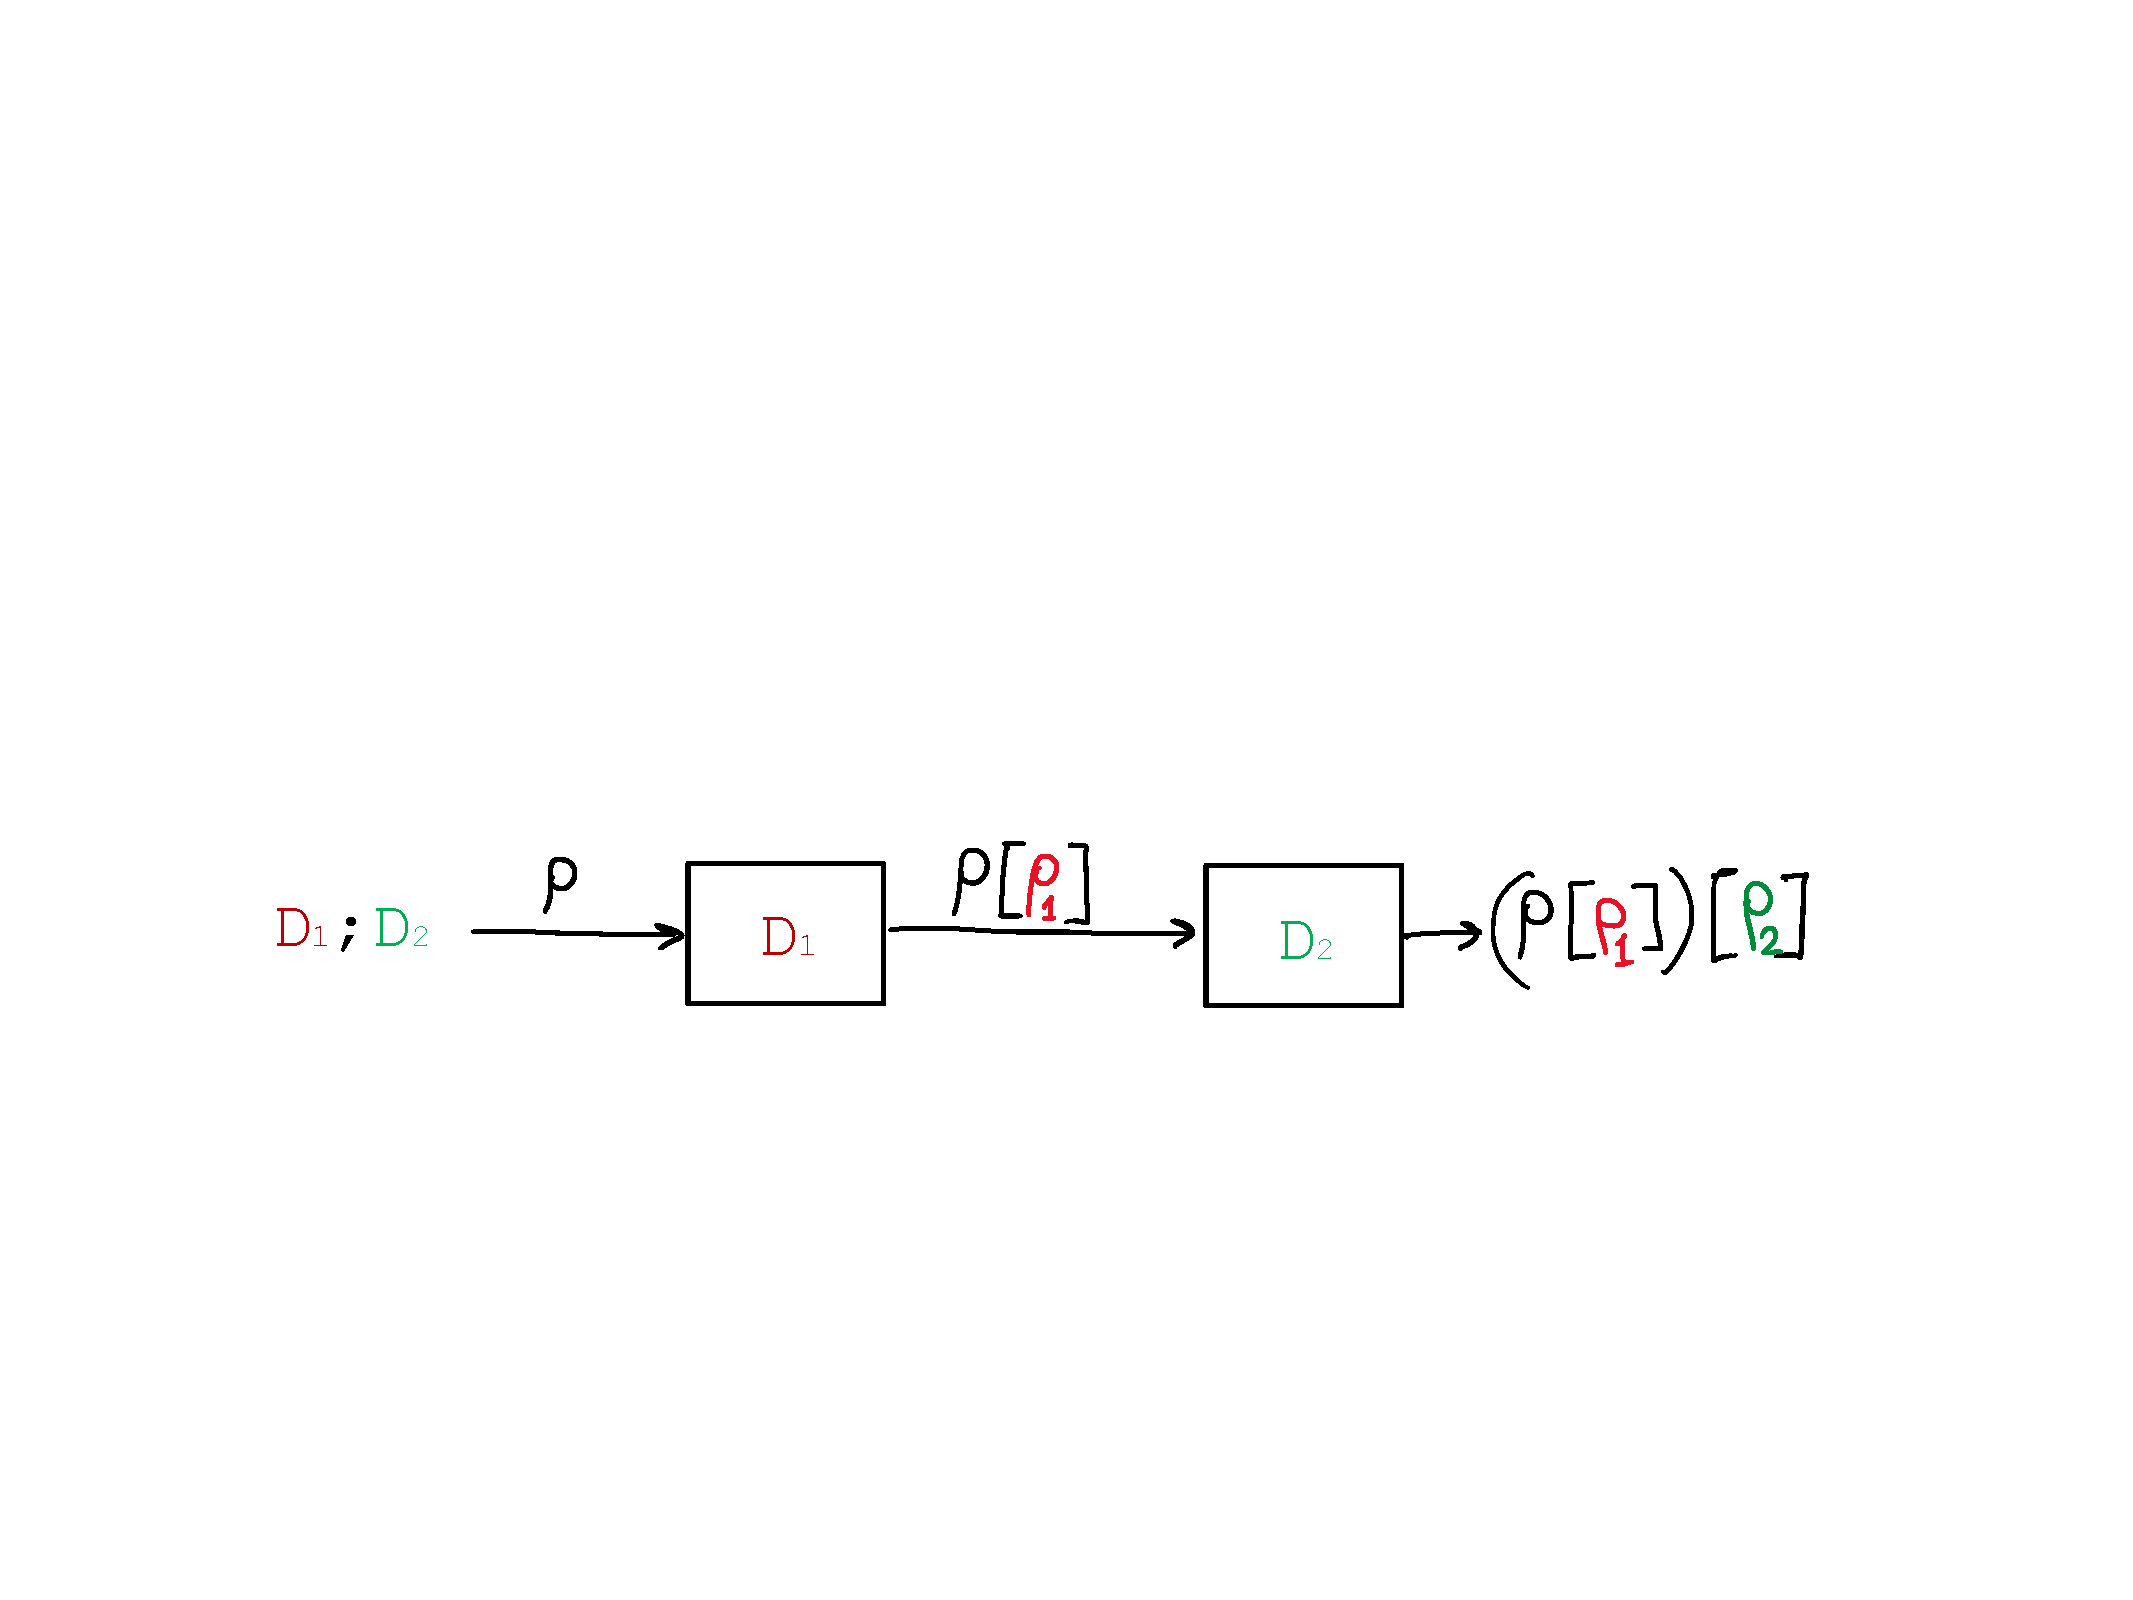
\includegraphics[width=\textwidth]{img/composizione_sequenziale.pdf}
	\end{figure}

	\noindent
	Un \textcolor{Green4}{\textbf{esempio}} di \textbf{composizione sequenziale}:
	\begin{figure}[!htp]
		\centering
		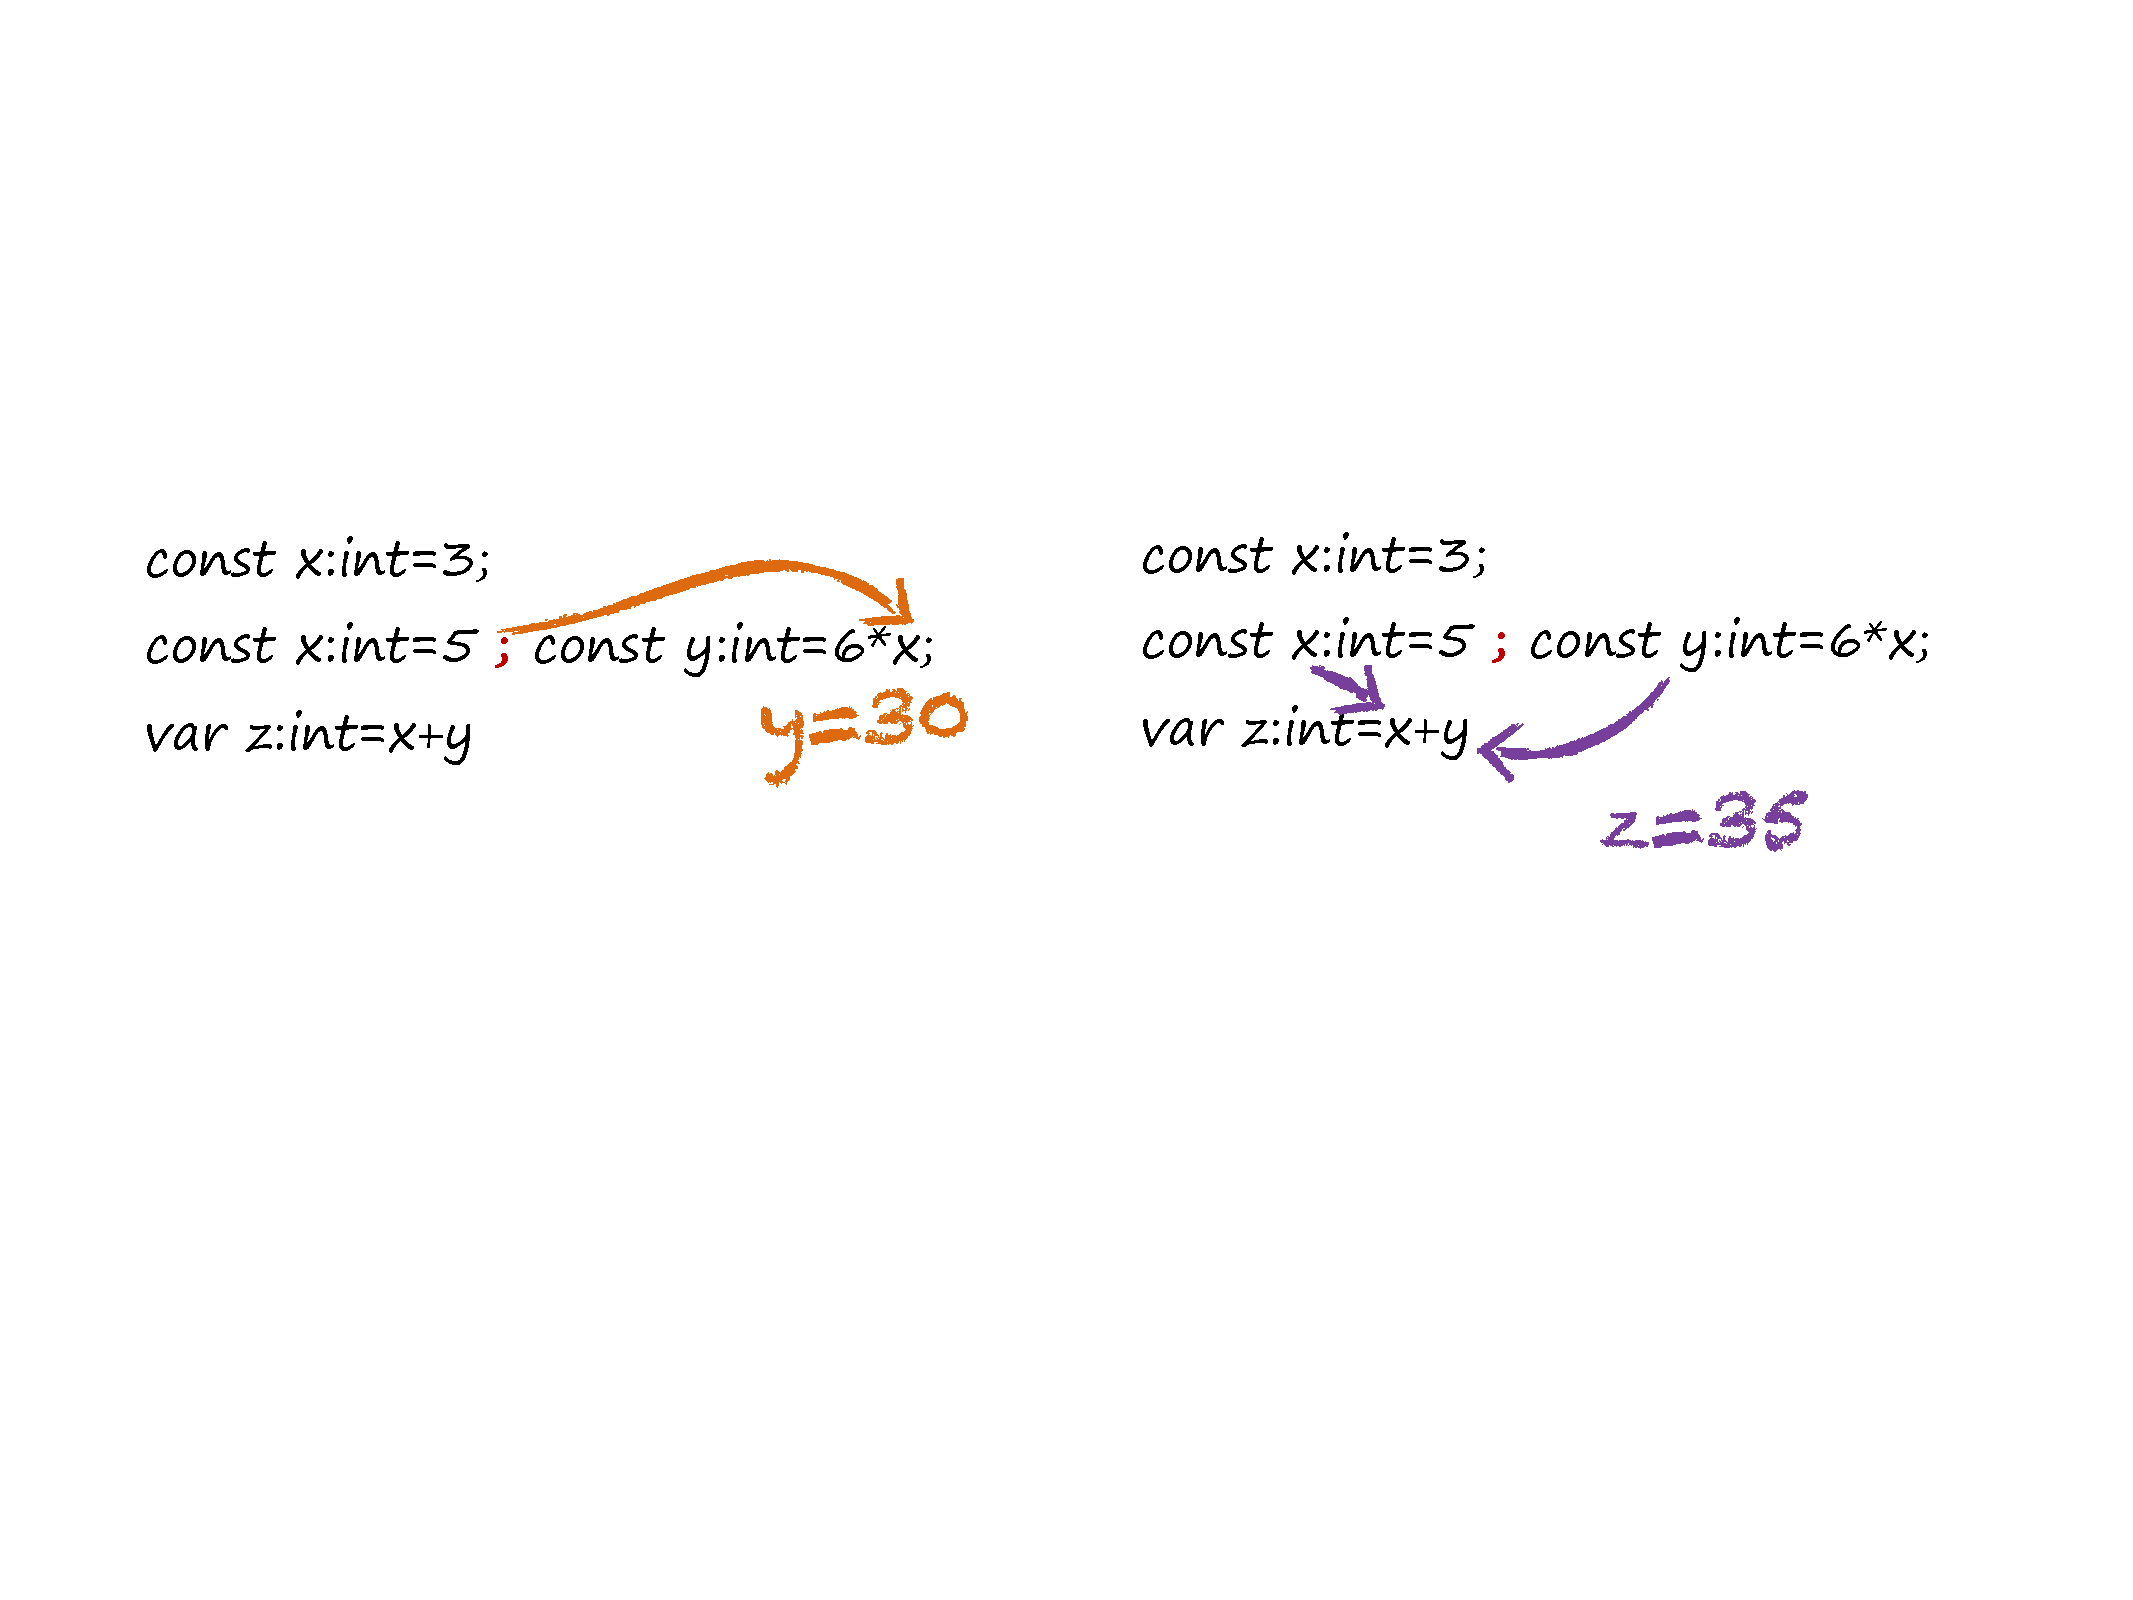
\includegraphics[width=\textwidth]{img/esempio_composizione_sequenziale.pdf}
	\end{figure}
	
	\noindent
	Al contrario, nella \textbf{composizione privata} la prima dichiarazione è appunto privata, esclusiva, per la seconda:
	\begin{figure}[!htp]
		\centering
		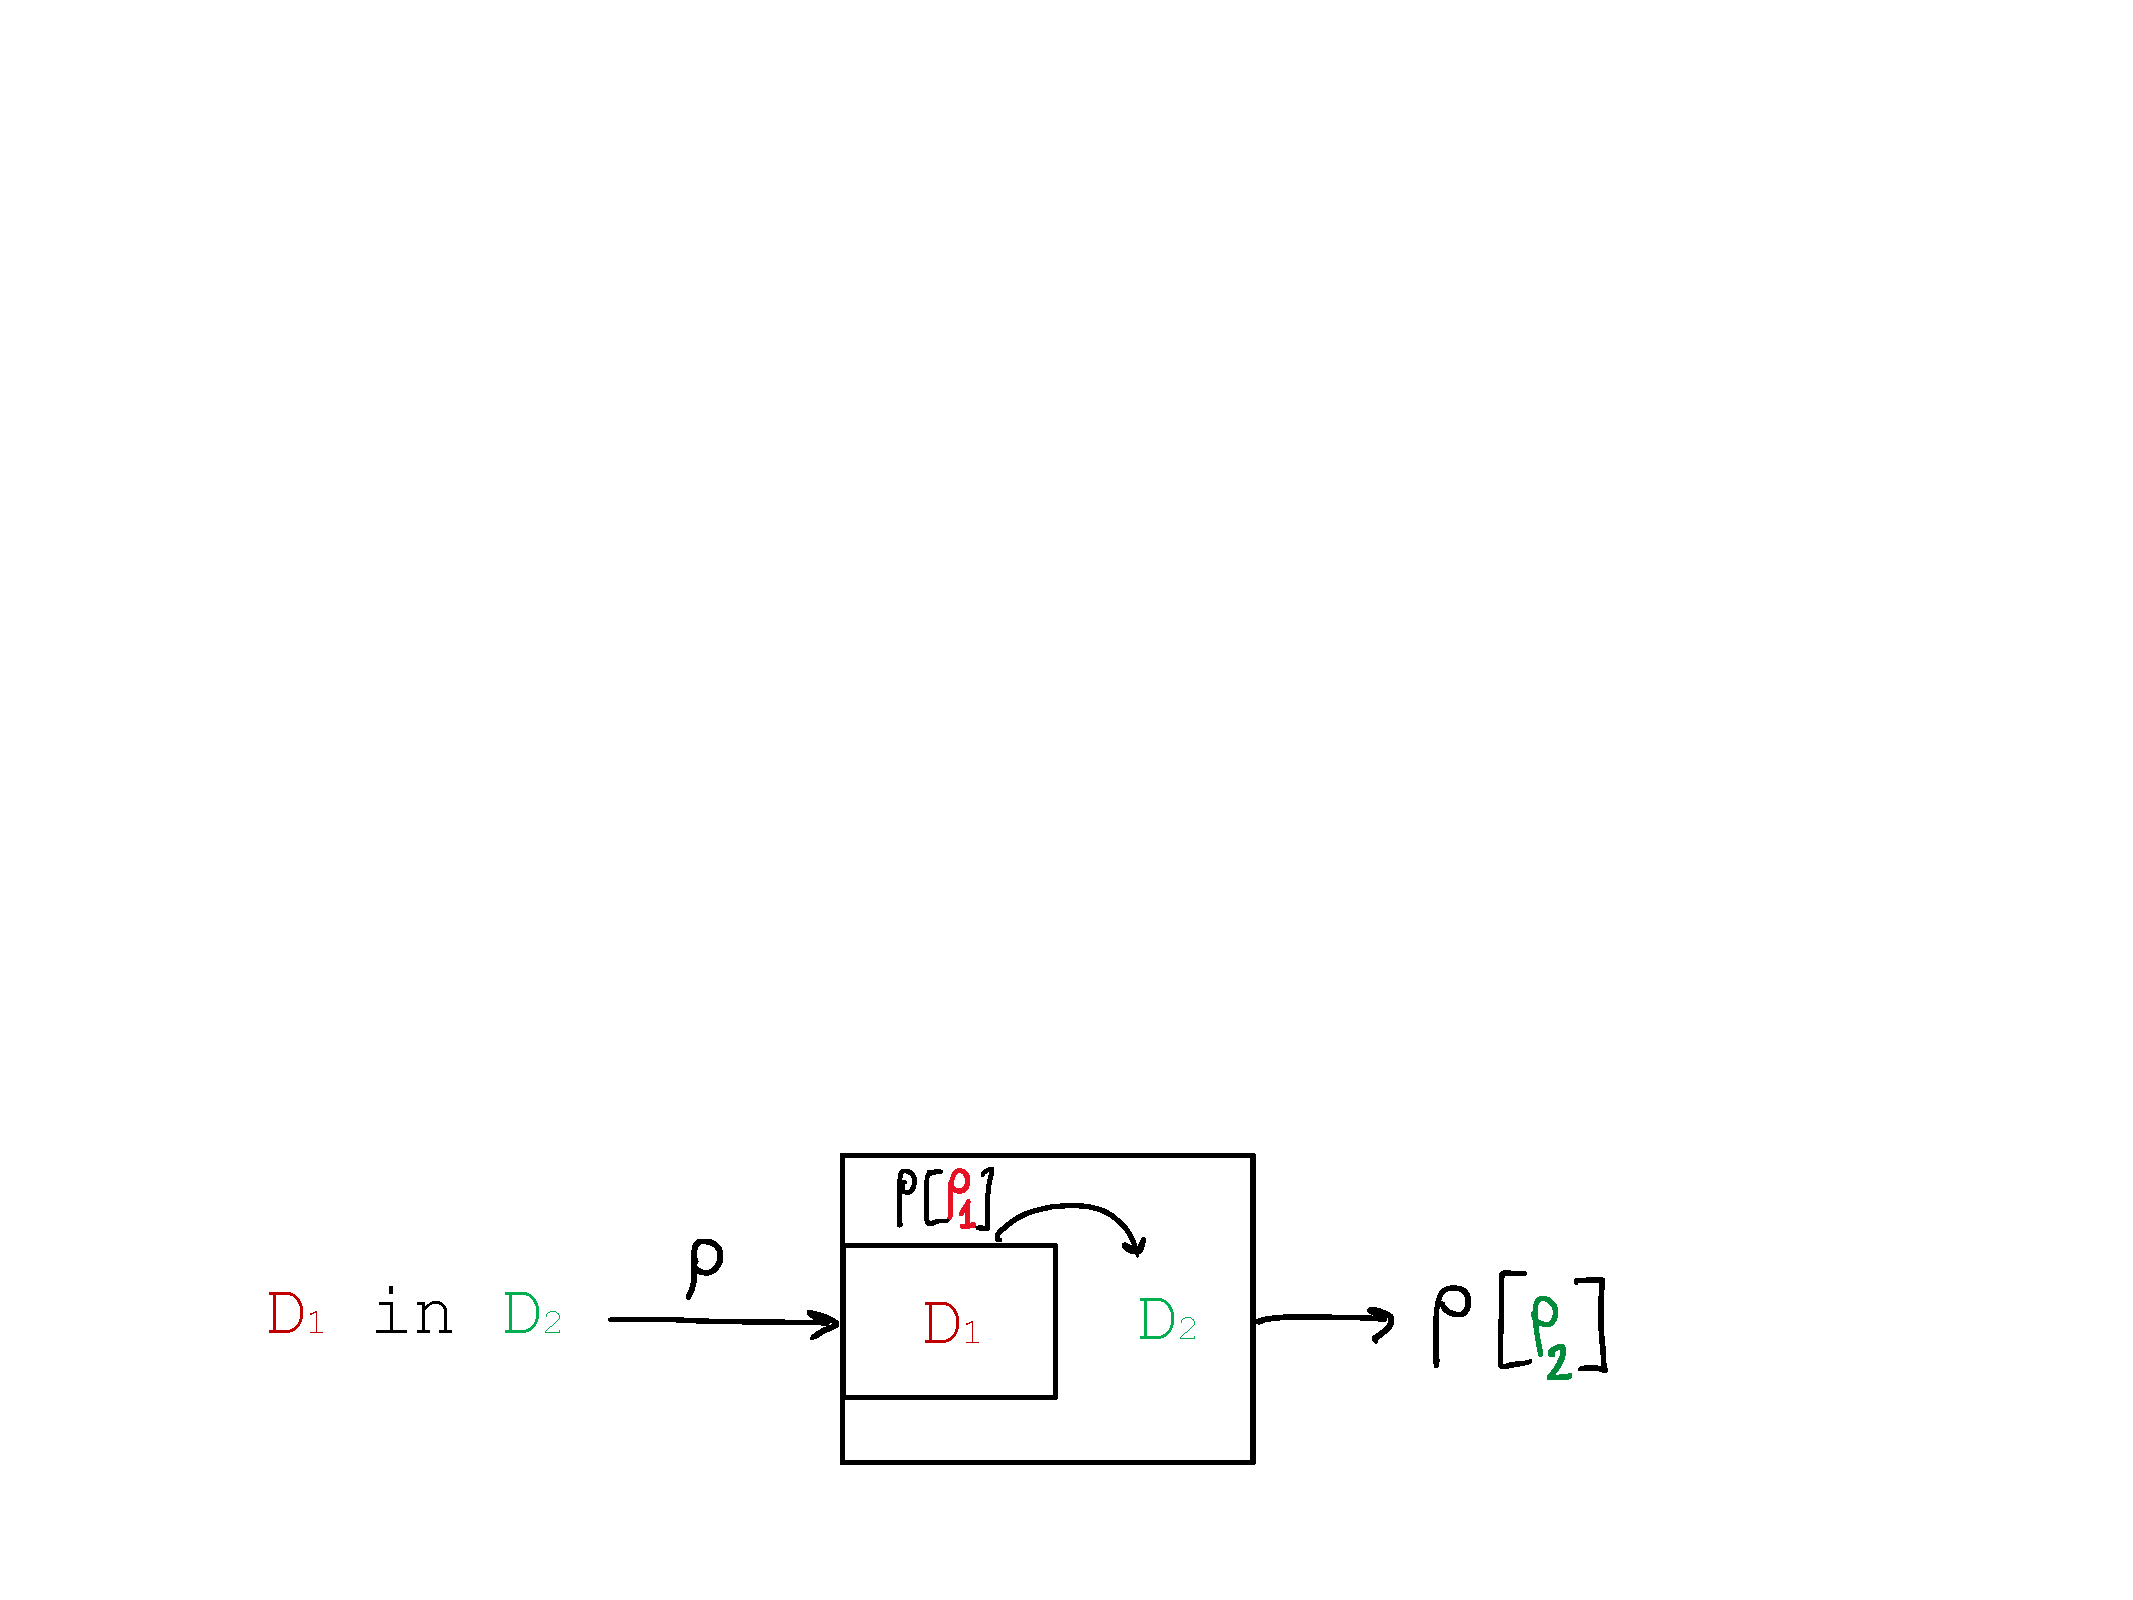
\includegraphics[width=\textwidth]{img/composizione_privata.pdf}
	\end{figure}

	\noindent
	Un \textcolor{Green4}{\textbf{esempio}} di \textbf{composizione privata}:
	\begin{figure}[!htp]
		\centering
		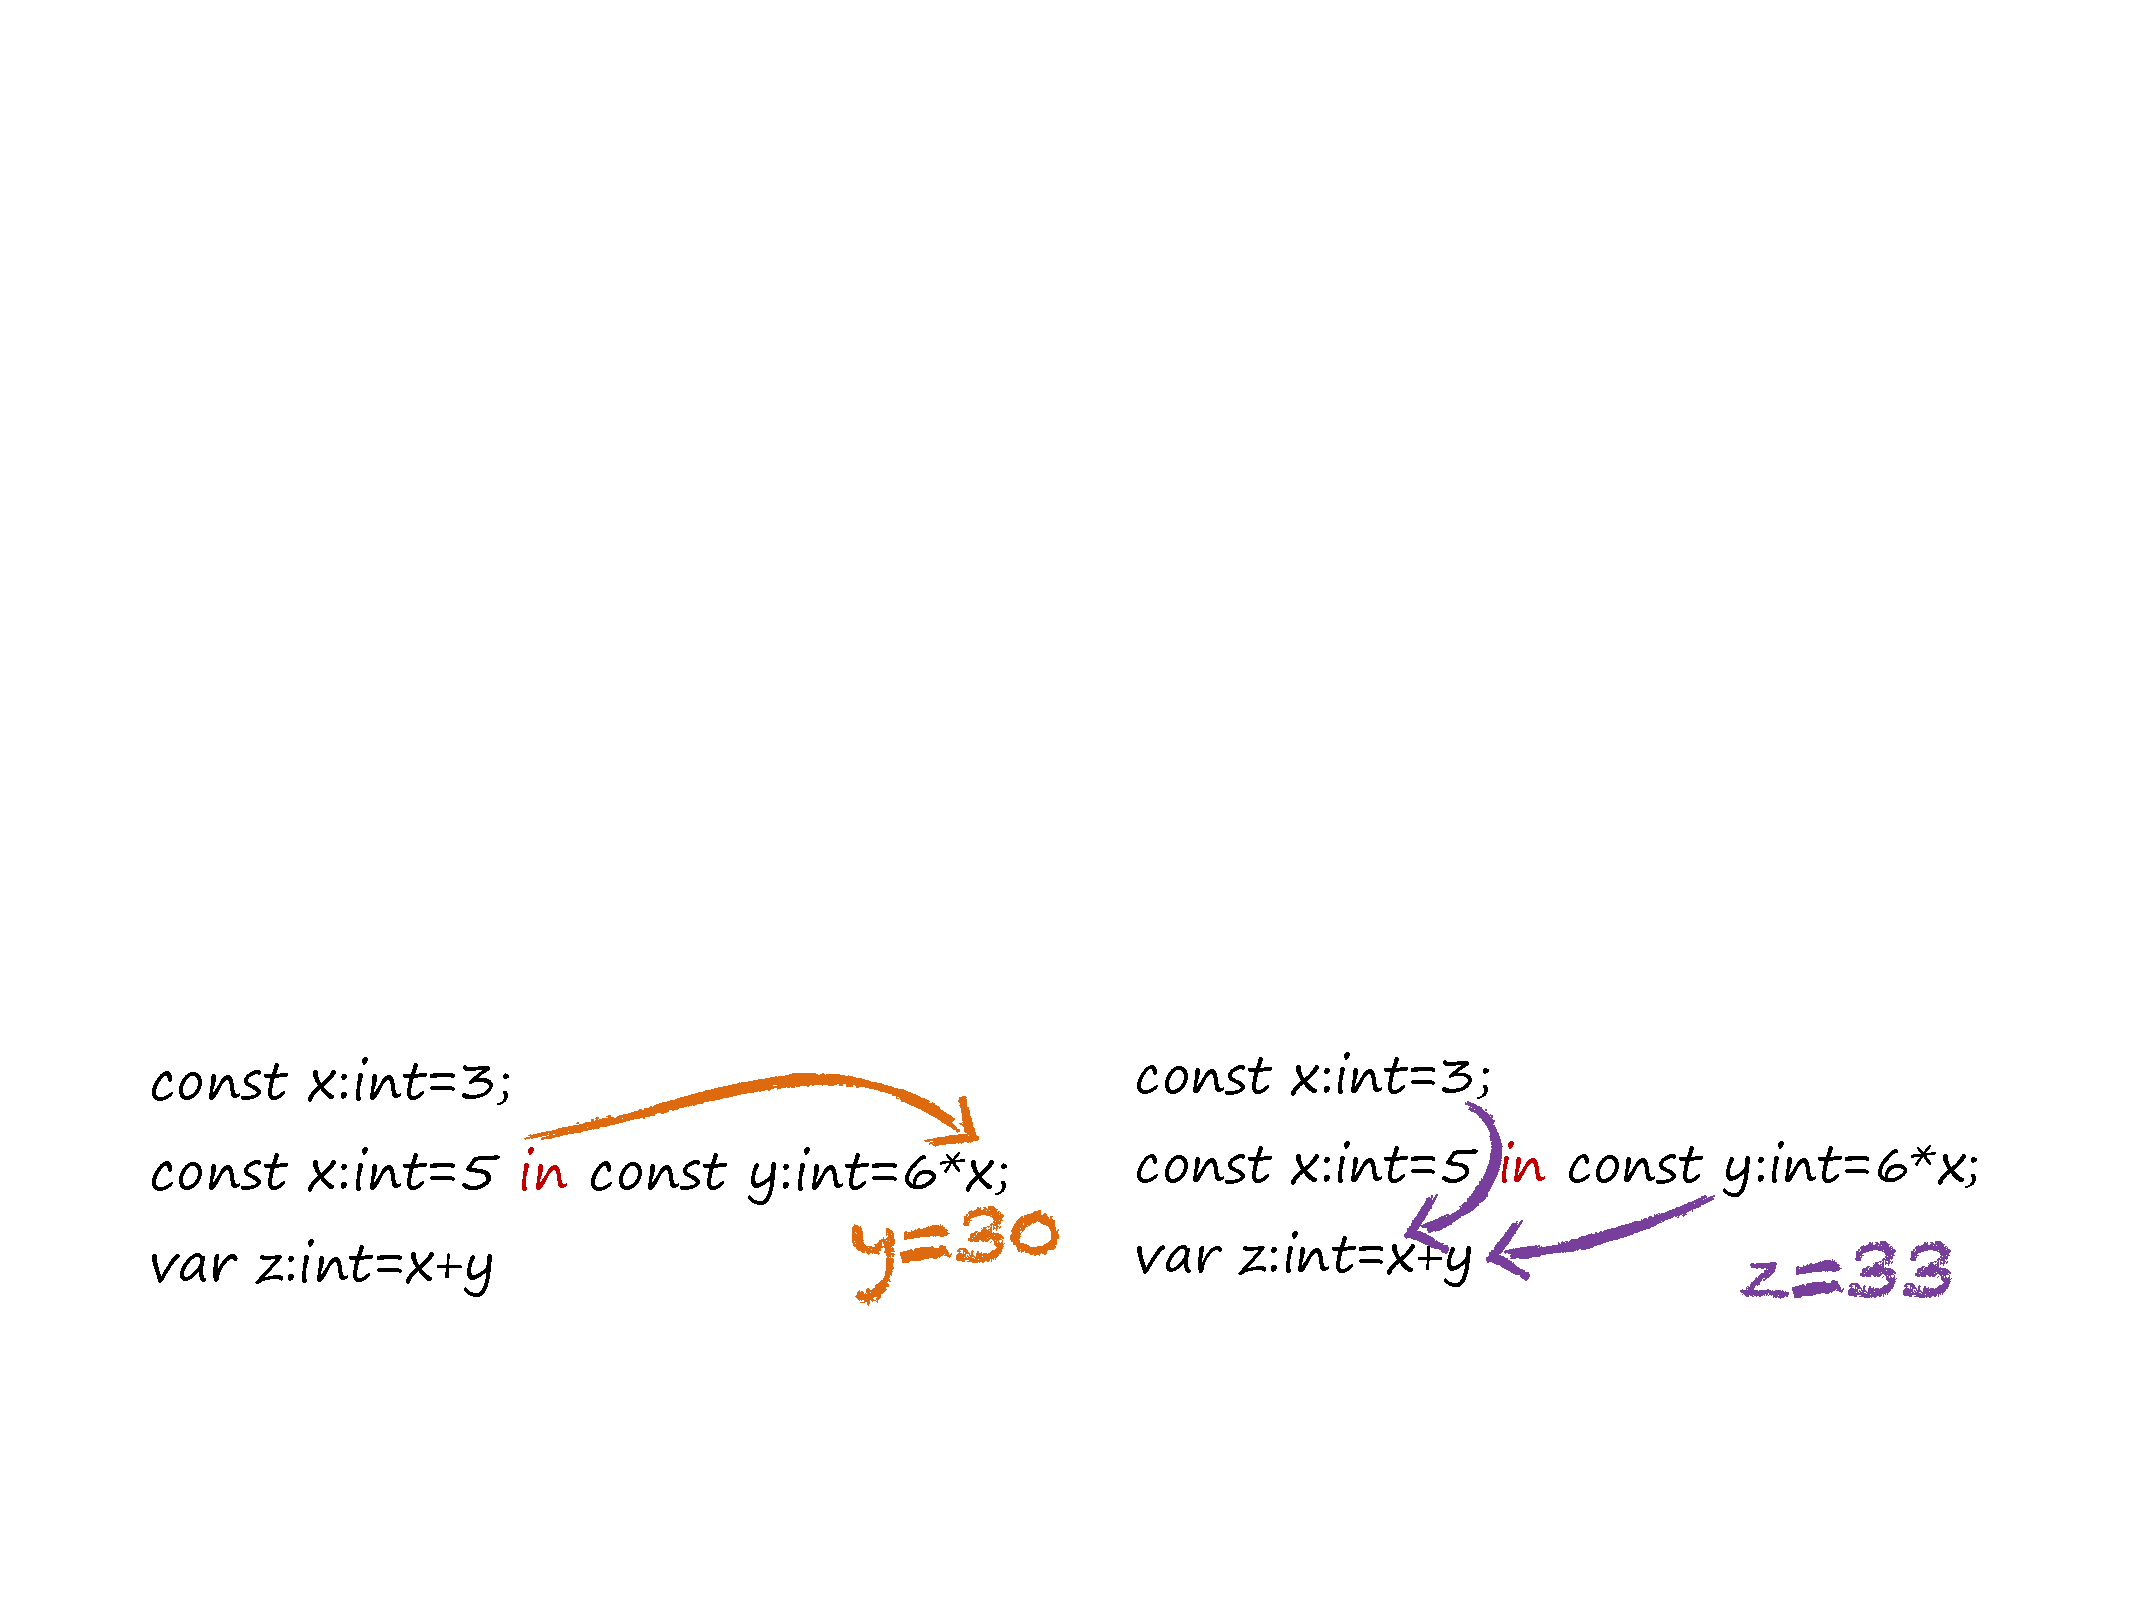
\includegraphics[width=\textwidth]{img/esempio_composizione_privata.pdf}
	\end{figure}\newpage
	
	\subsubsection{Identificatori definiti nelle dichiarazioni}\label{identificatori definiti}
	
	Si introducono gli \textcolor{Red3}{\textbf{identificatori definiti}}, ovvero identificatori in posizione di definizione. Si ricorda che l'obbiettivo primario delle dichiarazioni è quello di definire identificatori.\newline
	
	\noindent
	Quindi si definisce la funzione $DI$ (\emph{definite identificators}) che \textbf{associa ad ogni dichiarazione l'insieme degli identificatori} che definisce:
	\begin{equation*}
		DI: Dic \longrightarrow \wp\left(ID\right)
	\end{equation*}
	La definizione è induttiva sulla struttura delle dichiarazioni:
	\begin{itemize}
		\item La \textbf{\underline{dichiarazione nulla}} non definisce identificatori ed è un insieme vuoto:
		\begin{equation*}
			DI\left(\mathsf{nil}\right) = \emptyset
		\end{equation*}
		
		\item La \textbf{\underline{dichiarazione di costante}} definisce precisamente l'identificatore che sta dichiarando. Questo significa che dove questa dichiarazione è visibile, l'identificatore $x$ è legato a questa definizione:
		\begin{equation*}
			DI\left(\mathbf{const} \: \mathsf{x}: \tau = \mathrm{e}\right) = \left\{x\right\}
		\end{equation*}
		
		\item La \textbf{\underline{composizione sequenziale}} definisce tutto ciò che è definito nelle due dichiarazioni. Questo significa che all'esterno della composizione tutte le occorrenze di identificatori qui definiti sono legate:
		\begin{equation*}
			DI\left(d_{1} ; d_{2}\right) = DI\left(d_{1}\right) \cup DI\left(d_{2}\right)
		\end{equation*}
		
		\item La \textbf{\underline{composizione privata}} è particolare. Ciò che viene definito nella prima dichiarazione $d_{1}$ rimane privato e quindi non risulta legato all'esterno della composizione. Fuori dalla composizione è legato solo ciò che viene definito nella seconda dichiarazione $d_{2}$:
		\begin{equation*}
			DI\left(d_{1} \: \mathsf{in} \: d_{2}\right) = DI\left(d_{2}\right)
		\end{equation*}
		
		\item Il \textbf{\underline{valore terminale}}, ovvero gli ambienti, definiscono tutti gli identificatori per i quali hanno una associazione:
		\begin{equation*}
			DI\left(\rho\right) = V
		\end{equation*}
		Dove $V$ è il dominio di $\rho$.
	\end{itemize}\newpage
	
	\subsubsection{Identificatori liberi nelle dichiarazioni}\label{identificatori liberi}
	
	Al contrario degli identificatori definiti, gli \textcolor{Red3}{\textbf{identificatori liberi}} si trovano fuori dallo scope di una qualche dichiarazione/definizione.\newline
	
	\noindent
	Gli \textbf{identificatori liberi}, calcolati dalla funzione $FI$ (\emph{free identificators}), si possono ottenere anche sulle dichiarazioni, per induzione sulla struttura della grammatica. In questo caso, $FI$ \textbf{applicata ad una dichiarazione restituisce l'insieme degli identificatori liberi nella dichiarazione}:
	\begin{equation*}
		FI: Dic \longrightarrow \wp\left(Id\right)
	\end{equation*}
	In particolare:
	\begin{itemize}
		\item La \textbf{\underline{dichiarazione nulla}} non ha identificatori e non ne ha liberi dunque:
		\begin{equation*}
			FI\left(\mathsf{nil}\right) = \emptyset
		\end{equation*}
		
		\item La \textbf{\underline{identificatori liberi}} della dichiarazione di costante sono tutti quelli usati nell'espressione che inizializza l'identificatore. Questi identificatori devono essere definiti nell'ambiente di elaborazione perché si possa valutare l'espressione:
		\begin{equation*}
			FI\left(\mathbf{const} \: \mathsf{x}: \tau = \mathrm{e}\right) = FI\left(\mathrm{e}\right)
		\end{equation*}
		
		\item Il \textbf{\underline{caso delle due composizioni}} sono sicuramente liberi tutti gli identificatori della prima dichiarazione $d_{1}$. Sono inoltre liberi tutti gli identificatori che sono liberi nella seconda dichiarazione $d_{2}$ ma che non vengono definiti in $d_{1}$:
		\begin{gather*}
			FI\left(d_{1} ; d_{2}\right) = FI\left(d_{1}\right) \cup \left(FI\left(d_{2}\right) \setminus DI\left(d_{1}\right)\right) \\
			FI\left(d_{1} \: \mathsf{in} \: d_{2}\right) = FI\left(d_{1}\right) \cup \left(FI\left(d_{2}\right) \setminus DI\left(d_{1}\right)\right)
		\end{gather*}
		
		\item Un \textbf{\underline{ambiente non ha identificatori liberi}}, in quanto gli unici identificatori che contiene sono quelli per cui definisce delle associazioni:
		\begin{equation*}
			FI\left(\rho\right) = \emptyset
		\end{equation*}
	\end{itemize}\newpage
	
	\subsubsection{Semantica statica delle dichiarazioni}
	
	Per le dichiarazioni, la \textbf{semantica statica deve associare un ambiente statico ad ogni dichiarazione scritta correttamente} (chiamata ben formata). Le regole, sempre per quanto riguarda le dichiarazioni, dovranno avere la seguente forma:
	\begin{equation*}
		\mathcal{D}\mathrm{s}_{\mathrm{i}}: \:\: \textcolor{Red3}{\Delta\vdash_{V}} \:\: \mathrm{d}:\Delta
	\end{equation*}
	
	\noindent
	Vuol dire che nel sistema di regole è possibile associare l'ambiente statico $\Delta$ alla dichiarazione $d$, se questa è ben formata.\newline
	
	\noindent
	Si introducono qua di seguito le \textbf{regole}:
	\begin{itemize}
		\item La \textbf{dichiarazione vuota} genera un ambiente vuoto:
		\begin{equation*}
			\mathcal{D}\mathrm{s}_{1}: \:\: \textcolor{Red3}{\vdash} \:\: \mathrm{nil}:\emptyset
		\end{equation*}
		
		\item Con un \textbf{ambiente dinamico}, l'ambiente statico associato è quello compatibile, ovvero quello che associa agli identificatori esattamente i tipi dei valori che l'ambiente dinamico associa:
		\begin{equation*}
			\mathcal{D}\mathrm{s}_{2}: \:\: \textcolor{Red3}{\vdash} \:\: \rho:\Delta \hspace{1em} \mathrm{se} \hspace{1em} \rho \vdash_{\Delta}
		\end{equation*}
		
		\item Nella \textbf{dichiarazione di costante}, il tipo da associare è stabilito esplicitamente dalla dichiarazione. Quest'ultima viene detta ben formata se rispetta quanto scritto a pagina~\ref{ben formata} ed è esattamente del tipo $\tau$ presente nella dichiarazione. In tal caso l'ambiente statico corrispondente è esattamente l'associazione di $\tau$ all'identificatore definito $x$:
		\begin{equation*}
			\mathcal{D}\mathrm{s}_{3} : \dfrac{
				\Delta\vdash_{\mathrm{V}} \:\: \mathrm{e}:\tau
			}{
				\Delta\vdash_{\mathrm{V}} \:\: \mathbf{const} \:\: \mathrm{x}:\tau = \mathrm{e} : \left[\mathrm{x} \leftarrow \tau\right]
			}
		\end{equation*}
	\end{itemize}\newpage

	\noindent
	Si considerino due ambiente $\beta$, $\beta' \in Env$ dove $\beta : V, \beta' : V'$ (cioè compatibili) con $V,V' \subseteq Id$, dove:
	\begin{itemize}
		\item $\beta$ è definito sugli identificatori in $V$	
		\item $\beta'$ è definito sull'insieme di identificatori $V'$
	\end{itemize}
	L'aggiornamento dell'ambiente $\beta$ mediante l'ambiente $\beta'$ dà come risultato l'ambiente $\beta''\in Env$, denotato con $\beta\left[\beta'\right]$, definito come:
	\begin{equation*}
		\beta''\left(I\right) = \begin{cases}
			\beta'\left(I\right)	& \text{se } I \in V' \\
			\beta\left(I\right)		& \text{altrimenti}
		\end{cases}
	\end{equation*}
	In altre parole, \textbf{l'ambiente che aggiorna ha la precedenza, tutto quello di cui questo ambiente non parla rimane inalterato}.\newline
	
	\noindent
	Quindi, la regola della \textbf{\underline{composizione privata}} è la seguente:
	\begin{equation*}
		\mathcal{D}\mathrm{s}_{4} : \dfrac{
			\Delta\vdash_{\mathrm{V}} \: \mathrm{d}_{1}:\Delta_{1} \hspace{1em} \Delta\left[\Delta_{1}\right] \vdash_{V \cup V'} \: \mathrm{d}_{2} : \Delta_{2}
		}{
			\Delta\vdash_{\mathrm{V}} \: \mathrm{d}_{1} \hspace{1em} \mathbf{in} \hspace{1em} \mathrm{d}_{2}:\Delta_{2}
		}
	\end{equation*}
	
	\noindent
	In cui $V'$ è il dominio dell'ambiente $\Delta_{1}$. Nelle premesse si trova:
	\begin{itemize}
		\item L'ambiente statico $\Delta_{1}$ associato alla dichiarazione $d_{1}$ se questa è ben formata. Successivamente, questo ambiente viene utilizzato per aggiornare l'ambiente contestuale con le nuove associazioni create da $d_{1}$.
		
		\item L'ambiente statico risultante viene utilizzato per associare l'ambiente $\Delta_{2}$ alla dichiarazione $d_{2}$. A questo punto, l'ambiente associato alla dichiarazione composta è solo l'ambiente associato alla dichiarazione $d_{2}$, in quanto $d_{1}$ (e quindi $\Delta_{1}$) è esclusivamente visibile/utilizzabile per l'elaborazione di $d_{2}$.
	\end{itemize}

	\noindent
	La \textbf{semantica statica per la \underline{composizione sequenziale}} ha la seguente regola:
	\begin{equation*}
		\mathcal{D}\mathrm{s}_{5} : \dfrac{
			\Delta\vdash_{\mathrm{V}} \: \mathrm{d}_{1}:\Delta_{1} \hspace{1em} \Delta\left[\Delta_{1}\right] \vdash_{V \cup V'} \: \mathrm{d}_{2} : \Delta_{2}
		}{
			\Delta\vdash_{\mathrm{V}} \: \mathrm{d}_{1} \mathbf{;} \mathrm{d}_{2}:\Delta_{1}\left[\Delta_{2}\right]
		}
	\end{equation*}
	
	\noindent
	In cui $V'$ è il dominio dell'ambiente $\Delta_{1}$. Nelle premesse:
	\begin{itemize}
		\item Si associa l'ambiente statico $\Delta_{1}$ corrispondente alla dichiarazione $d_{1}$;
		
		\item Si aggiorna l'ambiente esterno $\Delta$ con l'ambiente (punto precedente) $\Delta_{1}$ e quindi nell'ambiente risultante $\Delta\left[\Delta_{1}\right]$ si elabora la dichiarazione $d_{2}$, la quale viene associata all'ambiente $\Delta_{2}$.
		
		\item Quindi, l'ambiente che si associa alla dichiarazione composta sequenzialmente è esattamente $\Delta_{1}$ aggiornato da $\Delta_{2}$, ovvero $\Delta_{1}\left[\Delta_{2}\right]$
	\end{itemize}
	Questo significa che tutto quello che vene dichiarato nella dichiarazione composta è visibile all'esterno, tranne ciò che viene definito nella prima dichiarazione $d_{1}$ e ridefinito nella seconda dichiarazione $d_{2}$.\newpage
	
	\noindent
	Ad \textcolor{Green4}{\textbf{esempio}}, in $d_{1}$ un identificatore $x$ viene dichiarato booleano, mentre dentro $d_{2}$ lo stesso identificatore $x$ viene dichiarato intero. Questa seconda definizione riscrive la prima e all'esterno della composizione $x$ è visibile come intero e non più come booleano. Questo è quello che avviene:
	\begin{equation*}
		\begin{array}{lll}
			d_{1} & \mathsf{const} & x:\mathrm{bool} = true; \\
			d_{2} & \mathsf{const} & x:\mathrm{int} = 5; \: \mathsf{const} \hspace{1em} y: \mathrm{int} = 6*x
		\end{array}
	\end{equation*}
	
	\begin{figure}[!htp]
		\centering
		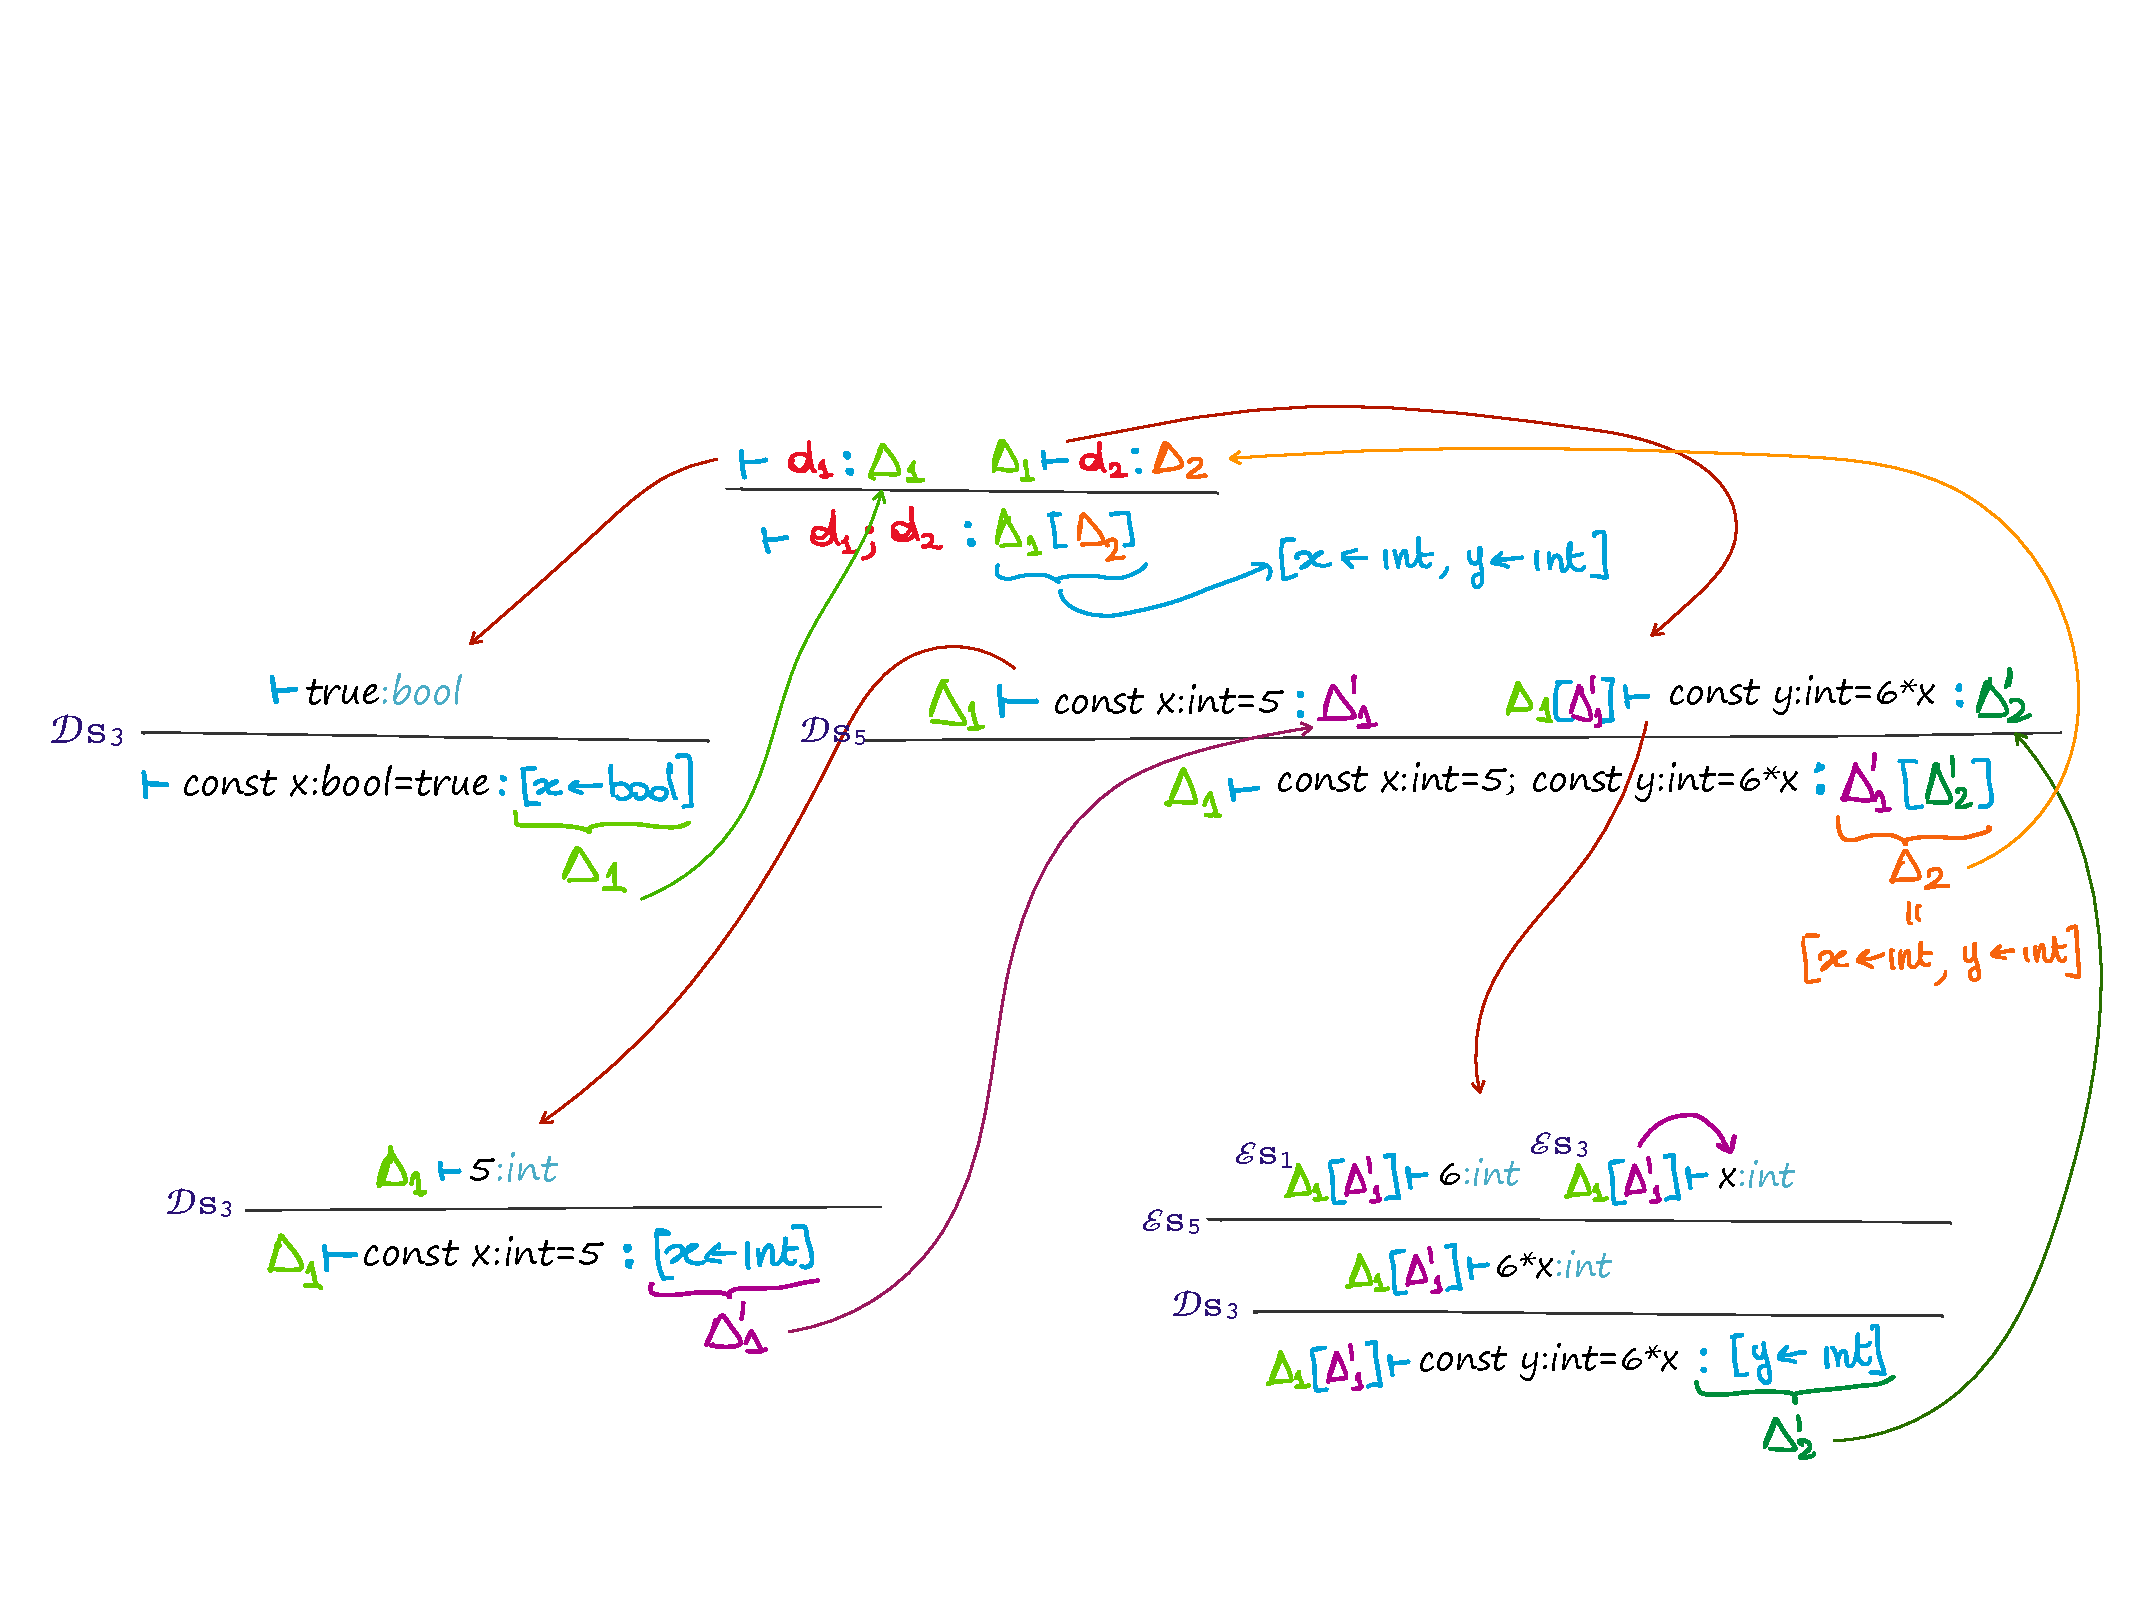
\includegraphics[width=1.3\textwidth]{img/semantica_statica_dichiarazioni-eg.pdf}
	\end{figure}\newpage
	
	\subsubsection{Semantica dinamica delle dichiarazioni}
	
	Si definisce l'insieme $\mathcal{D}$ come l'\textbf{insieme delle dichiarazioni con identificatori} (non con variabili) \textbf{da elaborare in ambienti dinamici}, ovvero in insiemi di associazioni tra identificatori e valori con metavariabile $d$.
	
	\begin{boxdef}
		L'\textbf{insieme delle dichiarazioni} $\mathcal{D}$ \textbf{è l'insieme di associazioni tra identificatori e valori (oggetti denotati) derivabili nella grammatica}: $d$.
	\end{boxdef}

	\noindent
	L'insieme dei valori derivabili è già stato definito e viene denotato $DVal$ (pagina~\pageref{DVal}), che per il momento può solo contenere interi, booleani e il tipo degli identificatori non definiti. Quindi, si definisce:
	\begin{itemize}
		\item L'\textbf{insieme delle configurazioni} $\Gamma$ come l'insieme delle configurazioni $\mathcal{D}$ da elaborare in ambienti;
		
		\item L'\textbf{insieme delle configurazioni} terminali $T$ sono ovviamente gli ambienti dinamici, i quali non hanno elementi da elaborare/valutare ulteriormente.
	\end{itemize}
	
	\begin{boxdef}
		Si definisce il \textcolor{Red3}{\textbf{sistema di transizione}} come:
		\begin{equation*}
			\Gamma = \mathcal{D}, T = Env
		\end{equation*}
	\end{boxdef}

	\noindent
	Le regole del sistema di transizione vanno definite induttivamente sulla struttura sintattica delle dichiarazioni. Le \textbf{regole} avranno la forma:
	\begin{equation*}
		\mathcal{D}_{\mathrm{i}} : \textcolor{Red3}{\rho \:\: \vdash_{\Delta}} \:\: \mathrm{d} \rightarrow_{\mathrm{d}} \mathrm{d}'
	\end{equation*}

	\begin{itemize}
		\item $\rho$ è l'\textbf{ambiente} nel quale viene elaborata la dichiarazione compatibile con l'ambiente statico $\Delta$;
		
		\item Il pedice $d$ della freccia serve ad indicare che la \textbf{regola è del sistema di transizione delle dichiarazioni}.
	\end{itemize}\newpage
	
	\subsection{Regole per l'elaborazione delle dichiarazioni}
	
	\begin{itemize}
		\item La prima regola è un \textbf{assioma} che evidenzia come la dichiarazione nulla viene elaborata nell'ambiente dinamico vuoto:
		\begin{equation*}
			\mathcal{D}_{1} : \:\: \vdash \:\: \mathbf{nil} \:\: \rightarrow_{\mathrm{d}} \emptyset
		\end{equation*}
	
		\item La seconda regola è un'\textbf{assioma} che evidenzia come la dichiarazione costante (ben formata) viene elaborata nell'ambiente che associa all'identificatore definito dalla dichiarazione, il valore inserito nella dichiarazione per l'inizializzazione.\newline
		Ovviamente, se nella dichiarazione l'identificatore viene inizializzato con un'espressione non valutata, è necessario prima valutare l'espressione così da arrivare ad un valore costante e poter applicare l'assioma:
		\begin{equation*}
			\mathcal{D}_{2}: \:\: \rho \:\: \vdash_{\Delta} \:\: \mathbf{const} \:\: \mathrm{x} : \tau = \mathrm{k} \rightarrow_{\mathrm{d}} \left[\mathrm{x} = \mathrm{k}\right]
		\end{equation*}
	
		\item La terza regola:
		\begin{equation*}
			\mathcal{D}_{3}: \dfrac{
				\rho \:\: \vdash_{\Delta} \:\: \mathrm{e} \rightarrow_{\mathrm{e}} \mathrm{e}'
			}{
				\rho \:\: \vdash_{\Delta} \:\: \mathbf{const} \:\: \mathrm{x} : \tau = \mathrm{e} \:\: \rightarrow_{\mathrm{d}} \:\: \mathbf{const} \:\: \mathrm{x} : \tau = \mathrm{e}'
			}
		\end{equation*}
	\end{itemize}
	Le seguenti regole riguardano la \textbf{composizione sequenziale}:
	\begin{itemize}
		\item La quarta regola dice di elaborare completamente la dichiarazione a sinistra in un ambiente $\rho$:
		\begin{equation*}
			\mathcal{D}_{4}: \dfrac{
				\rho \:\: \vdash_{\Delta} \:\: \mathrm{d} \rightarrow_{\mathrm{d}} \mathrm{d}'
			}{
				\rho \:\: \vdash_{\Delta} \:\: \mathrm{d} ; \mathrm{d}_{1} \rightarrow_{\mathrm{d}} \mathrm{d}'; \mathrm{d}_{1}
			}
		\end{equation*}
		
		\item La quinta regola segue la precedente poiché qui è necessario valutare la dichiarazione a destra ed elaborarla in un ambiente esterno $\rho$ aggiornato da quello restituito dalla prima dichiarazione $\rho_{0}$, ovvero $\rho\left[\rho_{0}\right]$:
		\begin{equation*}
			\mathcal{D}_{5} : \dfrac{
				\rho\left[\rho_{0}\right] \:\: \vdash_{\Delta\left[\Delta_{0}\right]} \:\: \mathrm{d}_{1} \rightarrow_{\mathrm{d}} \mathrm{d}_{1'}
			}{
				\rho \:\: \vdash_{\Delta} \:\: \rho_{0} ; \mathrm{d}_{1} \rightarrow_{\mathrm{d}} \rho_{0} ; \mathrm{d}_{1'}
			}
		\end{equation*}
		
		\item La sesta regola conclude la composizione sequenziale ed è un \textbf{assioma} che consente di ottenere l'ambiente associato alla prima dichiarazione $\rho_{0}$ aggiornato dall'ambiente associato alla seconda dichiarazione $\rho_{1}$, ovvero $\rho_{0}\left[\rho_{1}\right]$:
		\begin{equation*}
			\mathcal{D}_{6} : \:\: \rho \:\: \vdash_{\Delta} \:\: \rho_{0} ; \rho_{1} \rightarrow_{\mathrm{d}} \rho_{0}\left[\rho_{1}\right]
		\end{equation*}
	\end{itemize}\newpage
	
	\noindent
	Per la \textbf{composizione privata}, le regole sono le stesse della composizione sequenziale. L'unica differenza è che quando entrambe le dichiarazioni sono state elaborate, solo l'ambiente associato alla seconda dichiarazione $\rho_{1}$ viene restituito come ambiente risultante:
	\begin{itemize}
		\item La settima regola:
		\begin{equation*}
			\mathcal{D}_{7} : \dfrac{
				\rho \:\: \vdash_{\Delta} \:\: \mathrm{d} \rightarrow_{\mathrm{d}} \mathrm{d}'
			}{
				\rho \:\: \vdash_{\Delta} \:\: \mathrm{d} \:\: \mathbf{in} \:\: \mathrm{d}_{1} \rightarrow_{\mathrm{d}} \mathrm{d}' \:\: \mathbf{in} \:\: \mathrm{d}_{1}
			}
		\end{equation*}
		
		\item L'ottava regola:
		\begin{equation*}
			\mathcal{D}_{8} : \dfrac{
				\rho\left[\rho_{0}\right] \:\: \vdash_{\Delta\left[\Delta_{0}\right]} \:\: \mathrm{d}_{1} \rightarrow_{\mathrm{d}} \mathrm{d}_{1'}
			}{
				\rho \:\: \vdash_{\Delta} \:\: \rho_{0} \:\: \mathbf{in} \:\: \mathrm{d}_{1} \rightarrow_{\mathrm{d}} \rho_{0} \:\: \mathbf{in} \:\: \mathrm{d}_{1'}
			}
		\end{equation*}
		
		\item La nona regola:
		\begin{equation*}
			\mathcal{D}_{9} : \:\: \rho \:\: \vdash_{\Delta} \:\: \rho_{0} \:\: \mathbf{in} \:\: \rho_{1} \rightarrow_{\mathrm{d}} \rho_{1}
		\end{equation*}
	\end{itemize}\newpage
	
	\subsection{Valutazione de equivalenza}
	
	Le regole elencate nel precedente paragrafo, definiscono formalmente cosa significa elaborare una dichiarazione.\newline
	
	\noindent
	Sia $\rho$ un ambiente dinamico appartenente all'insieme $Env$. Allora l'\textbf{elaborazione} è una funzione che prende una \textbf{dichiarazione sintattica}, ovvero un elemento nell'insieme $\mathcal{D}$, e gli \textbf{associa l'ambiente che esso rappresenta}.
	
	\begin{boxdef}
		L'\textcolor{Red3}{\textbf{elaborazione delle dichiarazioni}} formalmente si descrive nel seguente modo. \textbf{La valutazione è una funzione}:
		\begin{equation*}
			Elab: \mathcal{D} \longrightarrow Env
		\end{equation*}
		\textbf{Che descrive il comportamento dinamico delle dichiarazioni restituendo l'ambiente in cui esse sono elaborate:}
		\begin{equation*}
			Elab\left(d\right) = \rho \iff d \longrightarrow^{*} \rho
		\end{equation*}
	\end{boxdef}\:\newline

	\noindent
	Due dichiarazioni sono \textbf{equivalenti} quando potenzialmente sono \textbf{scritte con diversa sintassi}, ma \textbf{rappresentano lo stesso ambiente}, ovvero hanno lo stesso significato.
	
	\begin{boxdef}
		L'\textcolor{Red3}{\textbf{equivalenza di dichiarazioni}} formalmente si descrive nel seguente modo. \textbf{L'equivalenza di dichiarazioni è una relazione del tipo:}
		\begin{equation*}
			\equiv \subseteq \mathcal{D} \times \mathcal{D}
		\end{equation*}
		\textbf{Definita come segue:}
		\begin{equation*}
			d_{0} \equiv d_{1} \iff Elab\left(d_{0}\right) = Elab\left(d_{1}\right)
		\end{equation*}
	\end{boxdef}\:\newline
	
	\noindent
	Per \textcolor{Green4}{\textbf{esempio}}, la dichiarazione:
	\begin{equation*}
		\mathsf{const} \hspace{1em} x: \mathrm{int} = \left(3+5\right)*2
	\end{equation*}
	È equivalente alla dichiarazione:
	\begin{equation*}
		\mathsf{const} \hspace{1em} x: \mathrm{int} = \left(1+3\right)*4
	\end{equation*}
	Pur essendo due dichiarazioni \underline{sintatticamente} diverse.\newpage
	
	\subsection{Esempio completo di utilizzo delle regole}
	
	Solitamente, la risoluzione degli esercizi si concentra sul \textbf{partire da cosa dimostrare} e, ricorsivamente, arrivare a \textbf{determinare fatti sempre più semplici da dimostrare}, i quali \textbf{combinati danno la dimostrazione} iniziale cercata.\newline
	
	\noindent
	Questo sistema è deterministico, nel senso che in ogni istante è noto quale regola applicare. Quindi, si ottiene uno stile di prova logico-matematico basato su un sistema di transizione deterministico.\newline
	
	\noindent
	Qui di seguito viene proposto un esempio di come usare le regole della semantica dinamica per elaborare una dichiarazione.\newline
	
	\noindent
	Si consideri la seguente dichiarazione:
	\begin{figure}[!htp]
		\centering
		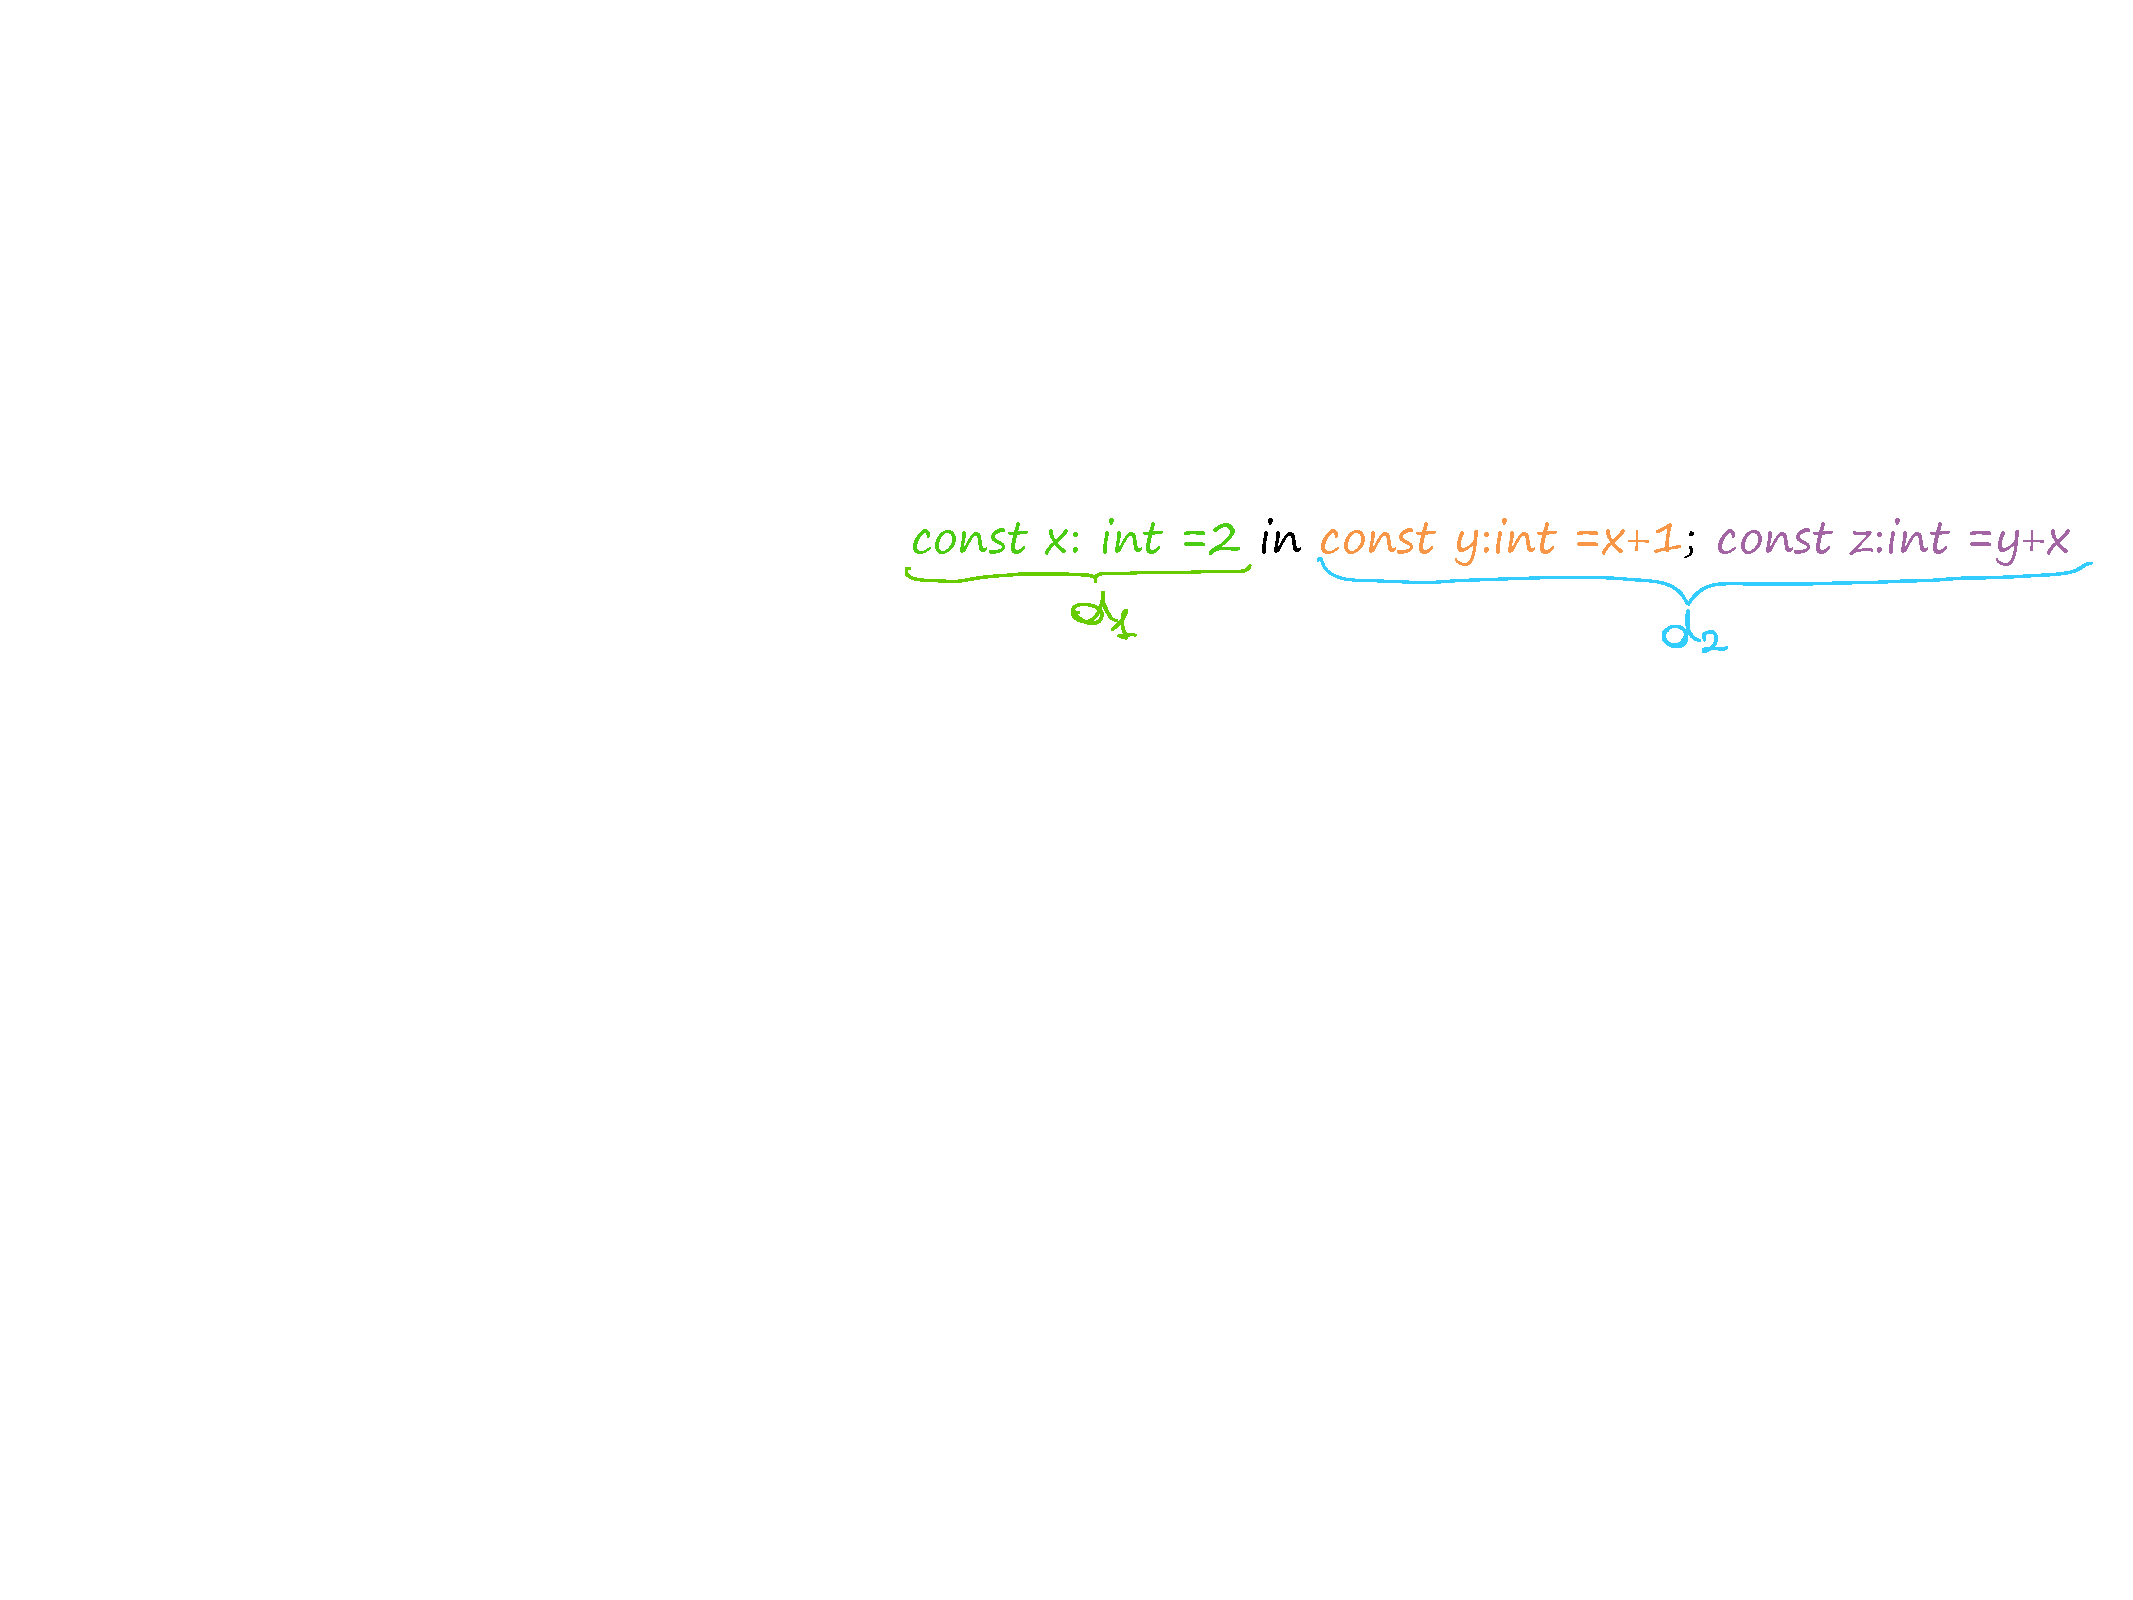
\includegraphics[width=.8\textwidth]{img/regola_dichiarazione-ex1.pdf}
	\end{figure}
	
	\noindent
	Si ha una composizione privata tra due dichiarazioni, di cui la seconda è a sua volta una composizione sequenziale di dichiarazioni. I passi saranno:
	\begin{enumerate}
		\item Elaborare $d_{1}$ in un ambiente;
		\item Elaborare $d_{2}$ utilizzando l'ambiente usato per $d_{1}$. Per farlo, viene elaborata prima la dichiarazione a sinistra e poi quella a destra nell'ambiente aggiornato.
	\end{enumerate}
	
	\begin{figure}[!htp]
		\centering
		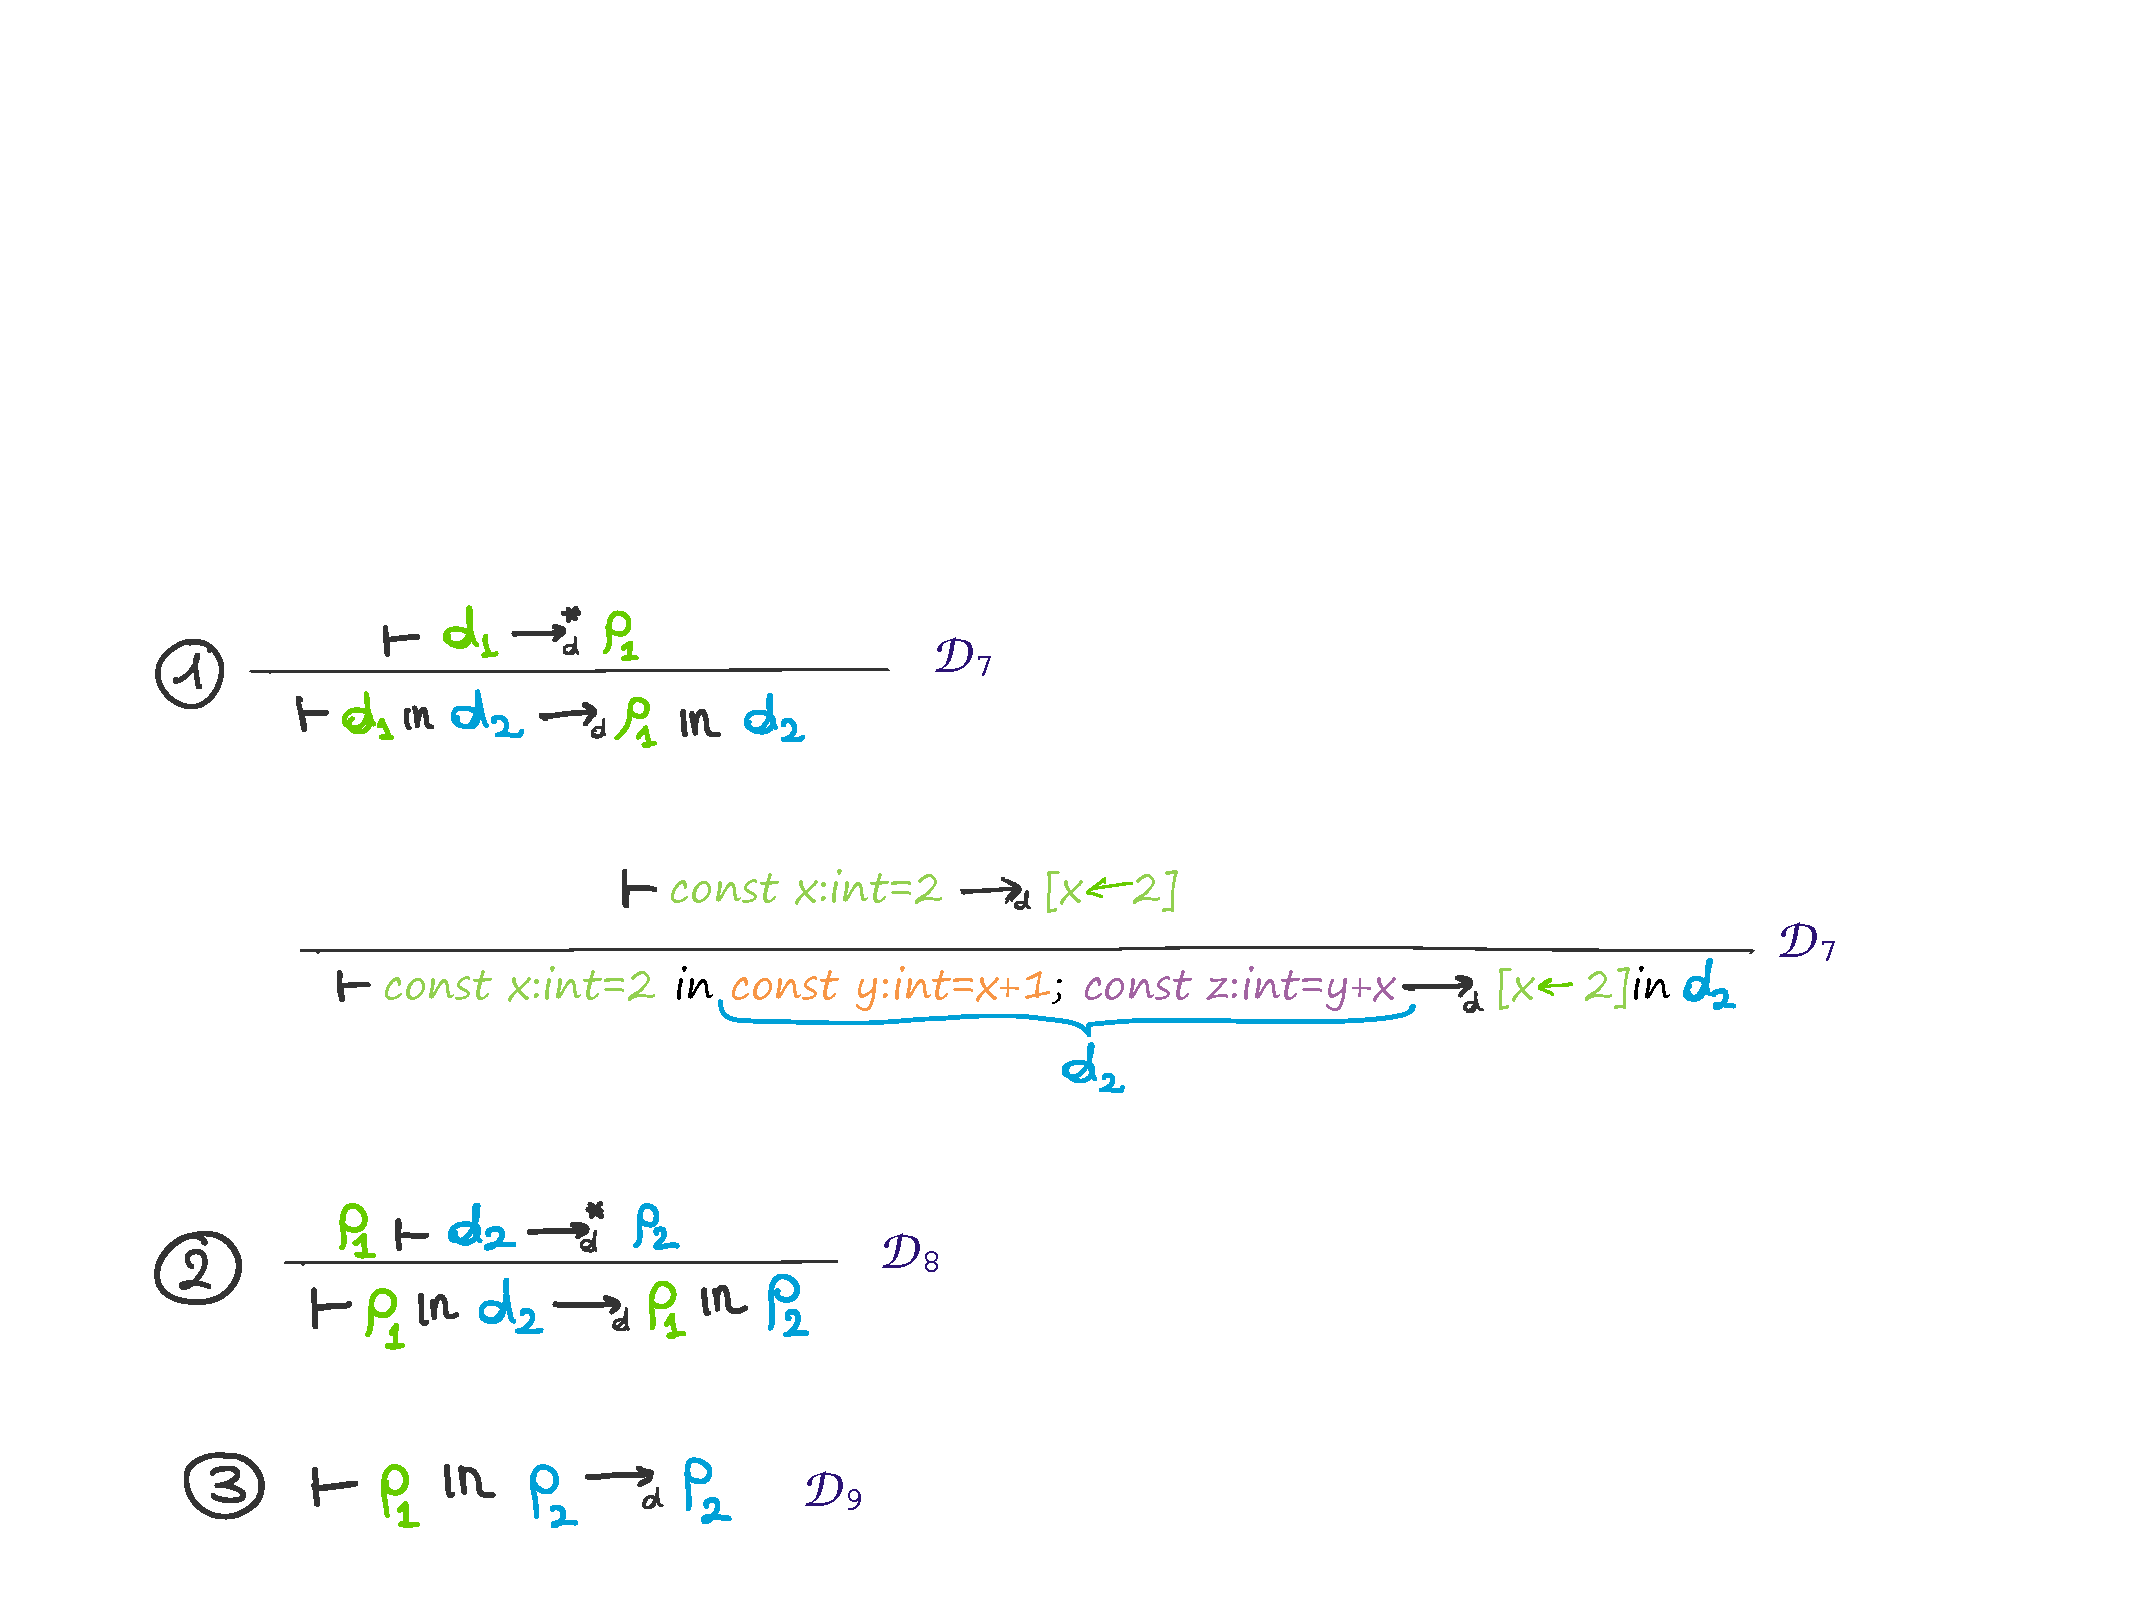
\includegraphics[width=\textwidth]{img/regola_espressione-ex2.pdf}
	\end{figure}\newpage

	\begin{figure}[!htp]
		\centering
		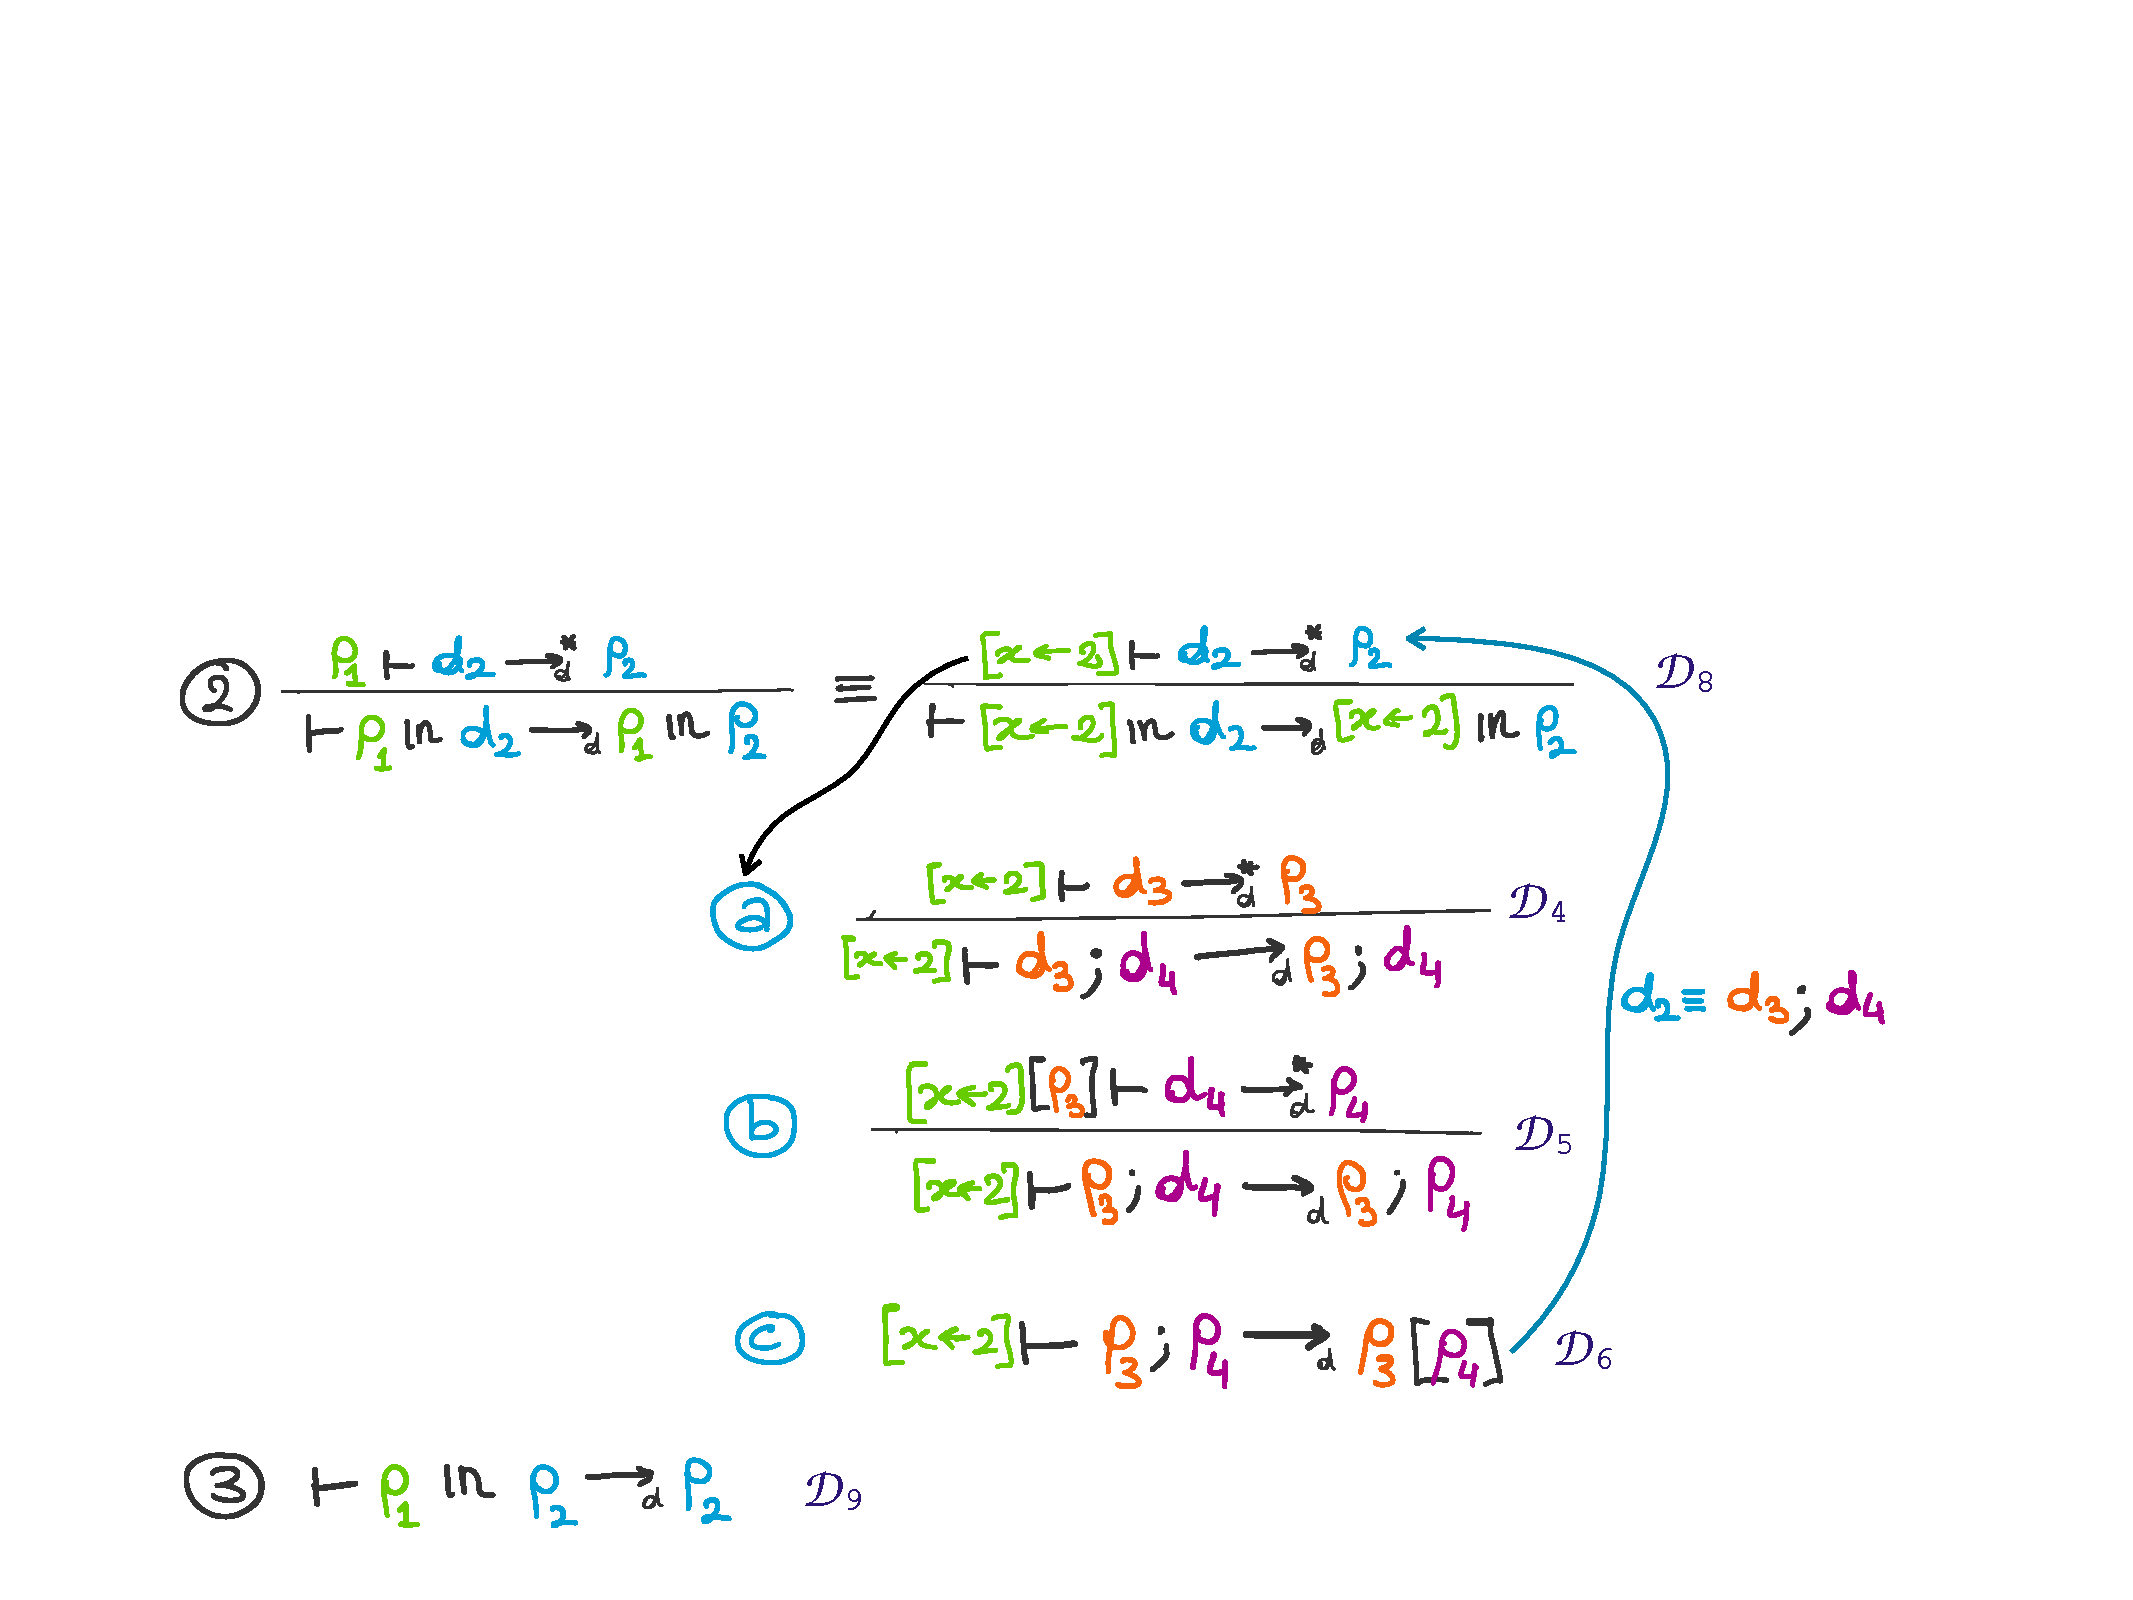
\includegraphics[width=\textwidth]{img/regola_espressione-ex3.pdf}
	\end{figure}

	\noindent
	Adesso si vuole dimostrare:
	
	\begin{figure}[!htp]
		\centering
		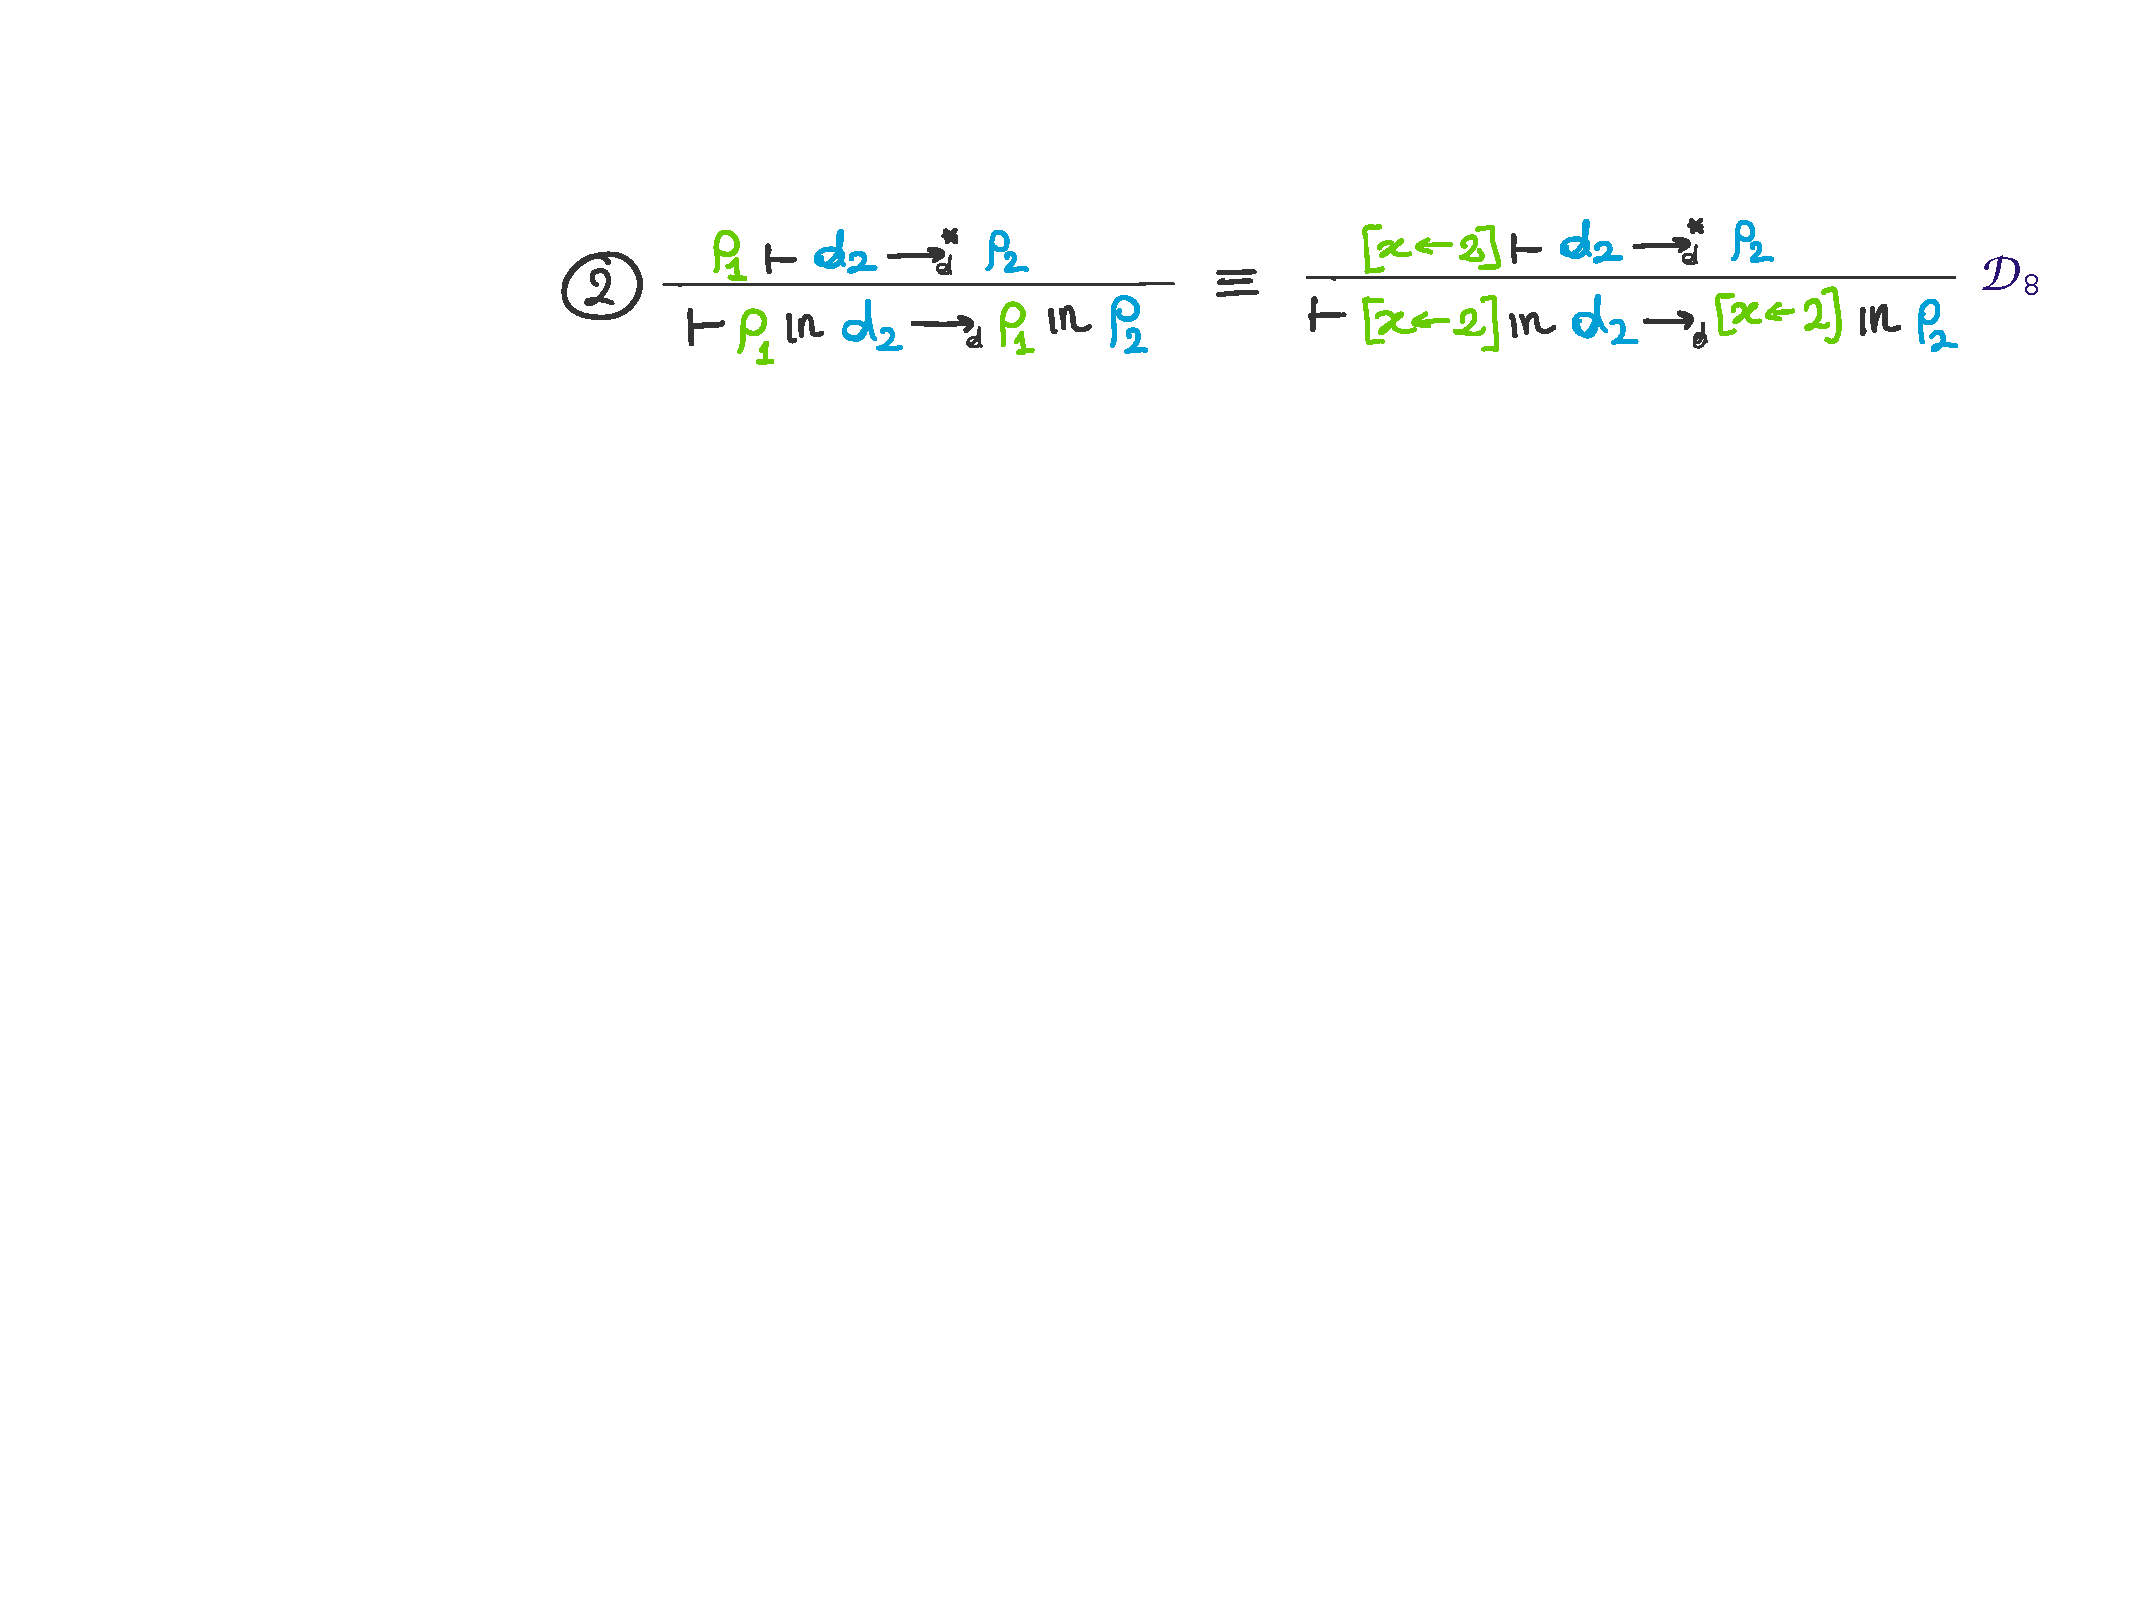
\includegraphics[width=\textwidth]{img/regola_espressione-ex4.pdf}
	\end{figure}
	
	\noindent
	Quindi, la dimostrazione per passi:
	
	\begin{figure}[!htp]
		\centering
		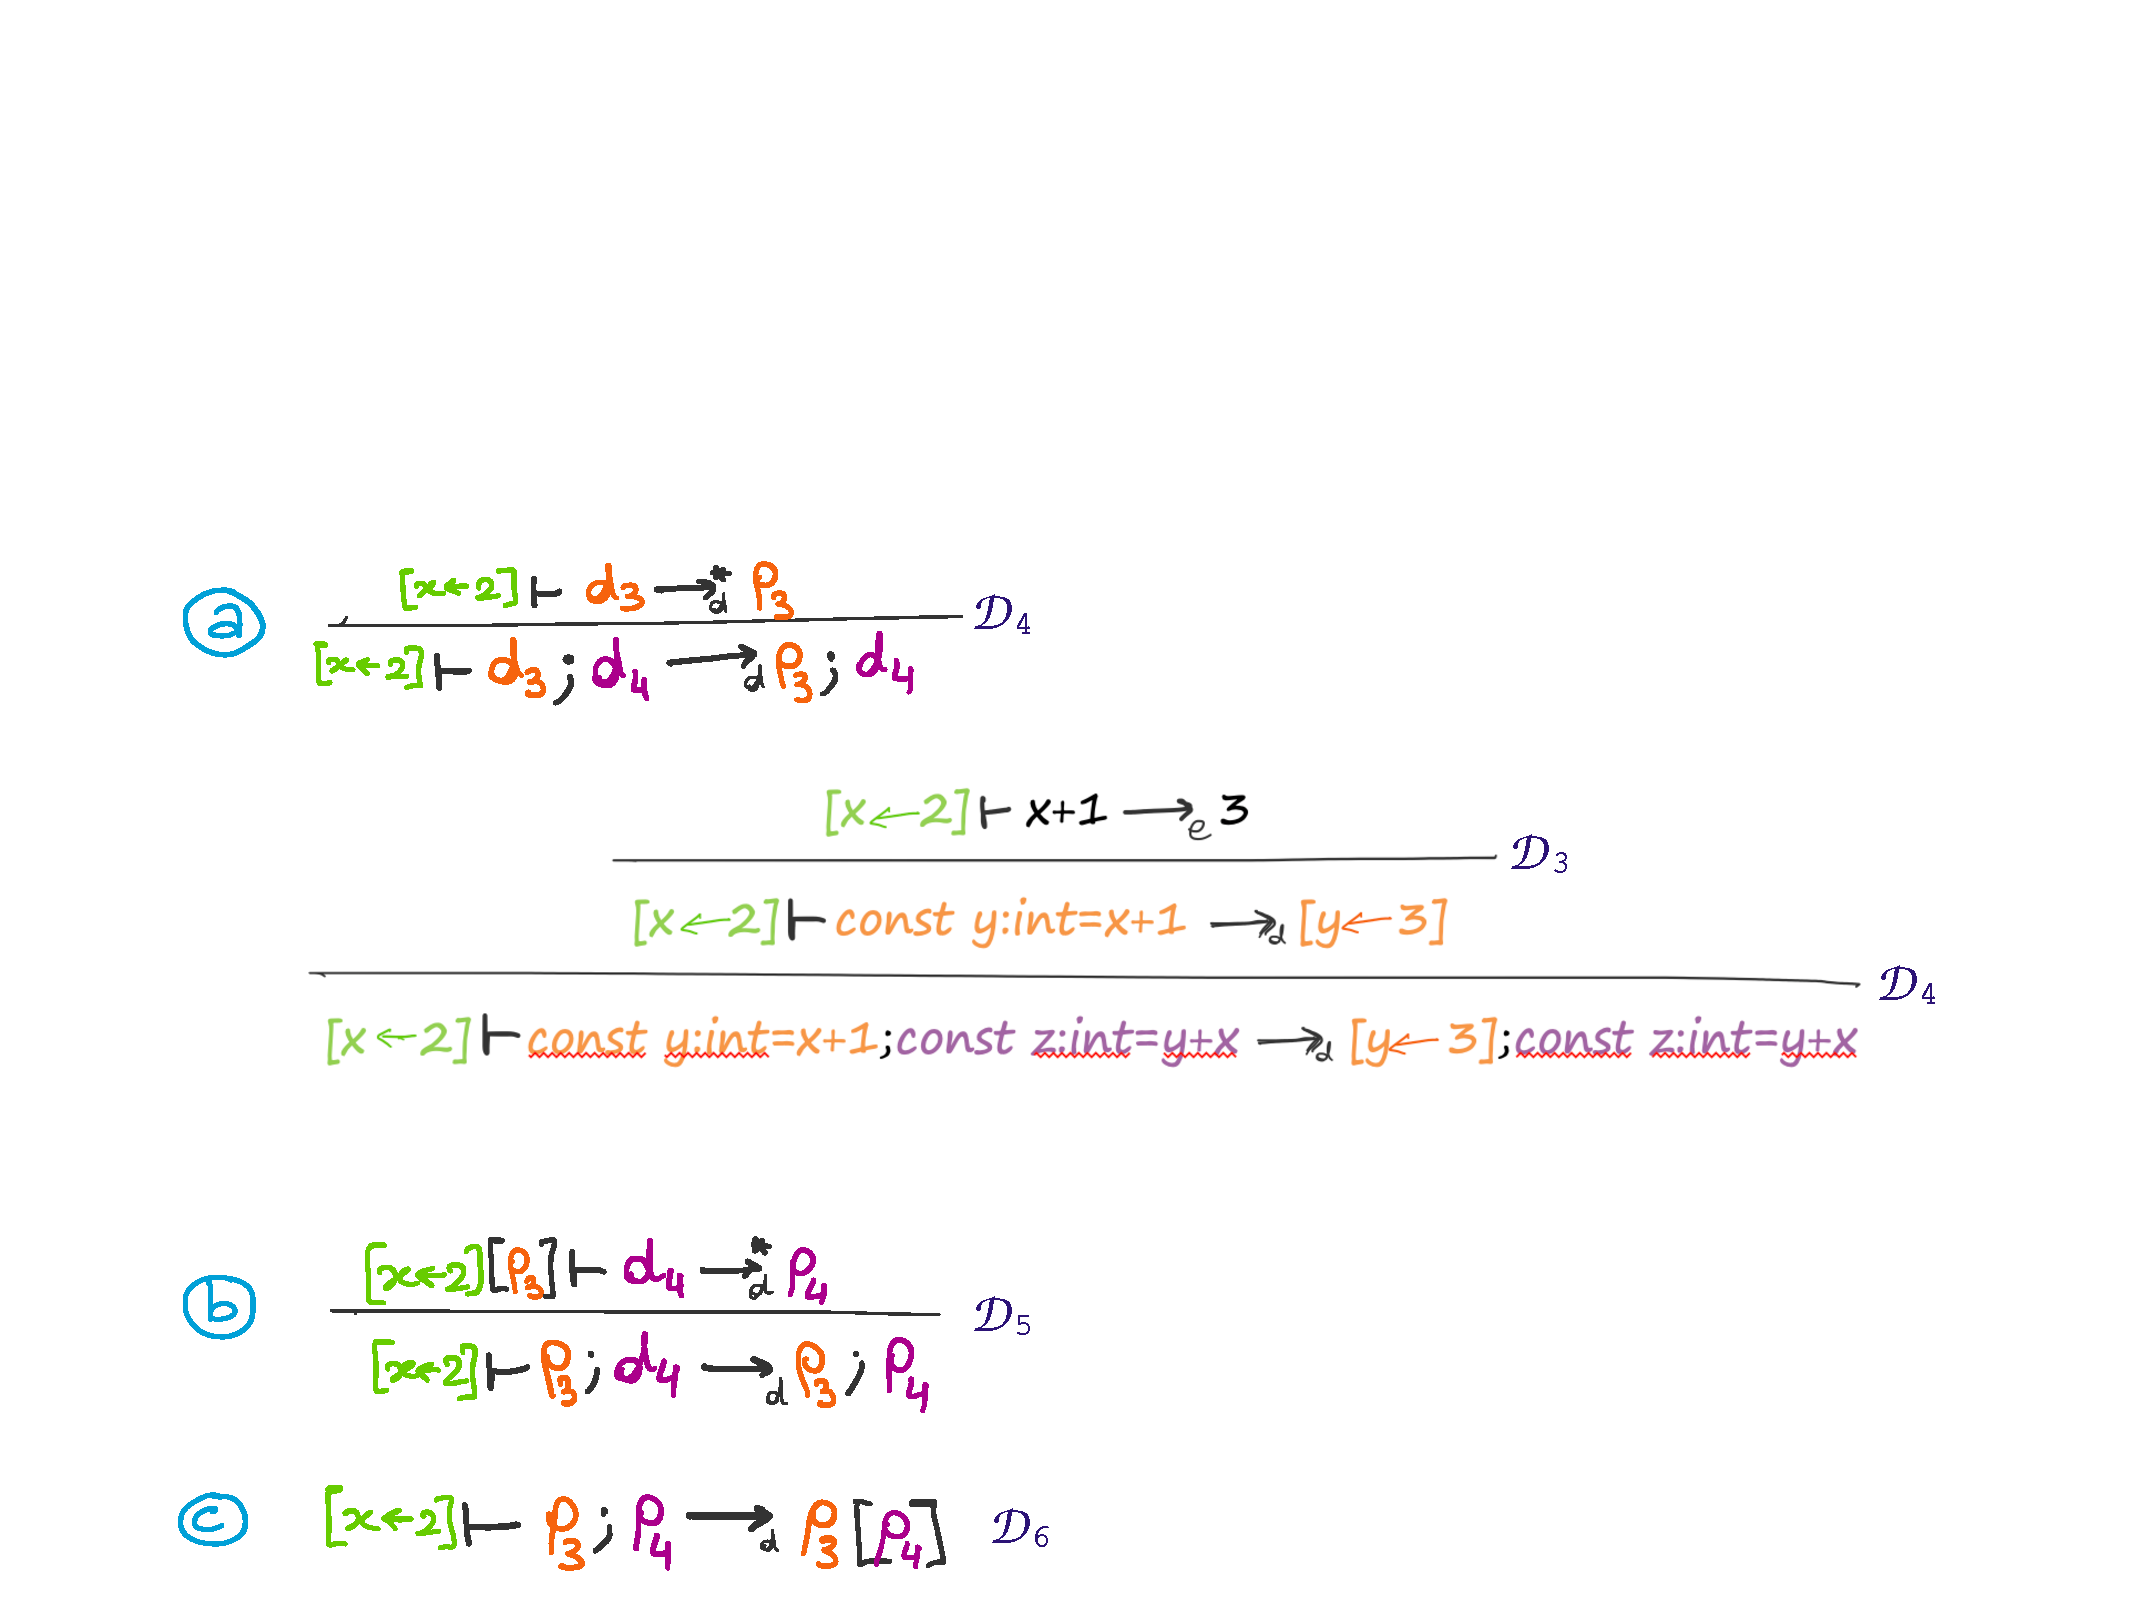
\includegraphics[width=\textwidth]{img/regola_espressione-ex5.pdf}
	\end{figure}\newpage

	\begin{figure}[!htp]
		\centering
		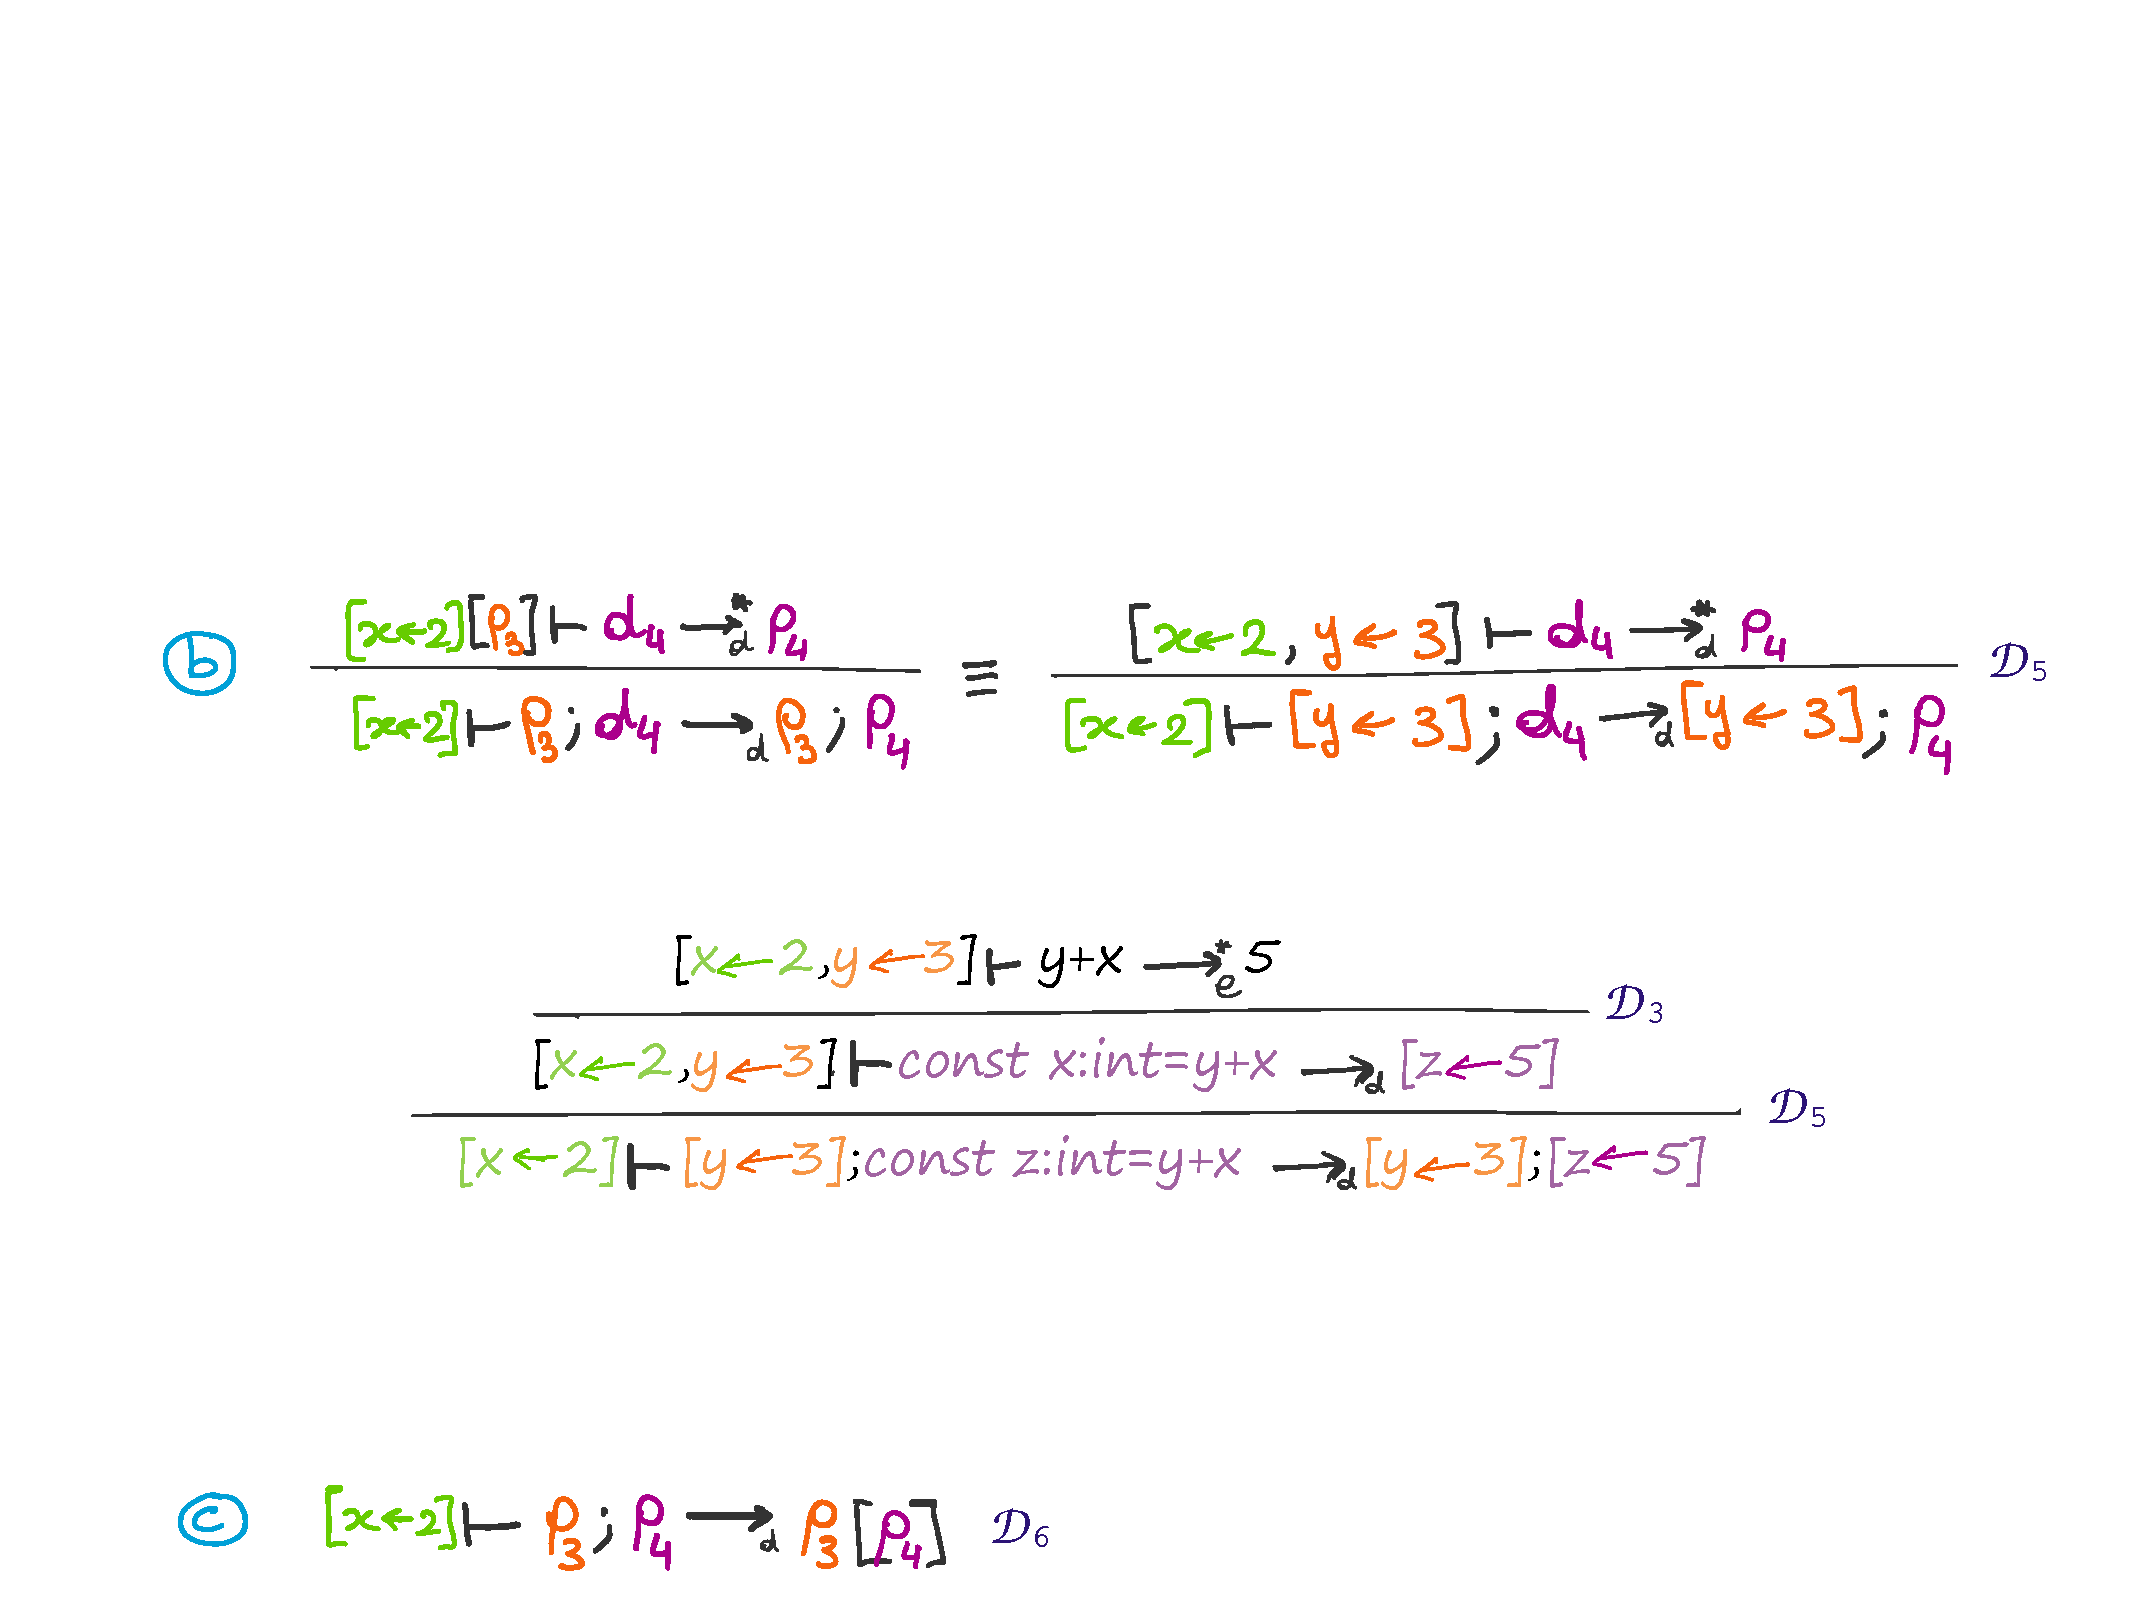
\includegraphics[width=\textwidth]{img/regola_espressione-ex6.pdf}
	\end{figure}

	\noindent
	Si conclude la dimostrazione:
	
	\begin{figure}[!htp]
		\centering
		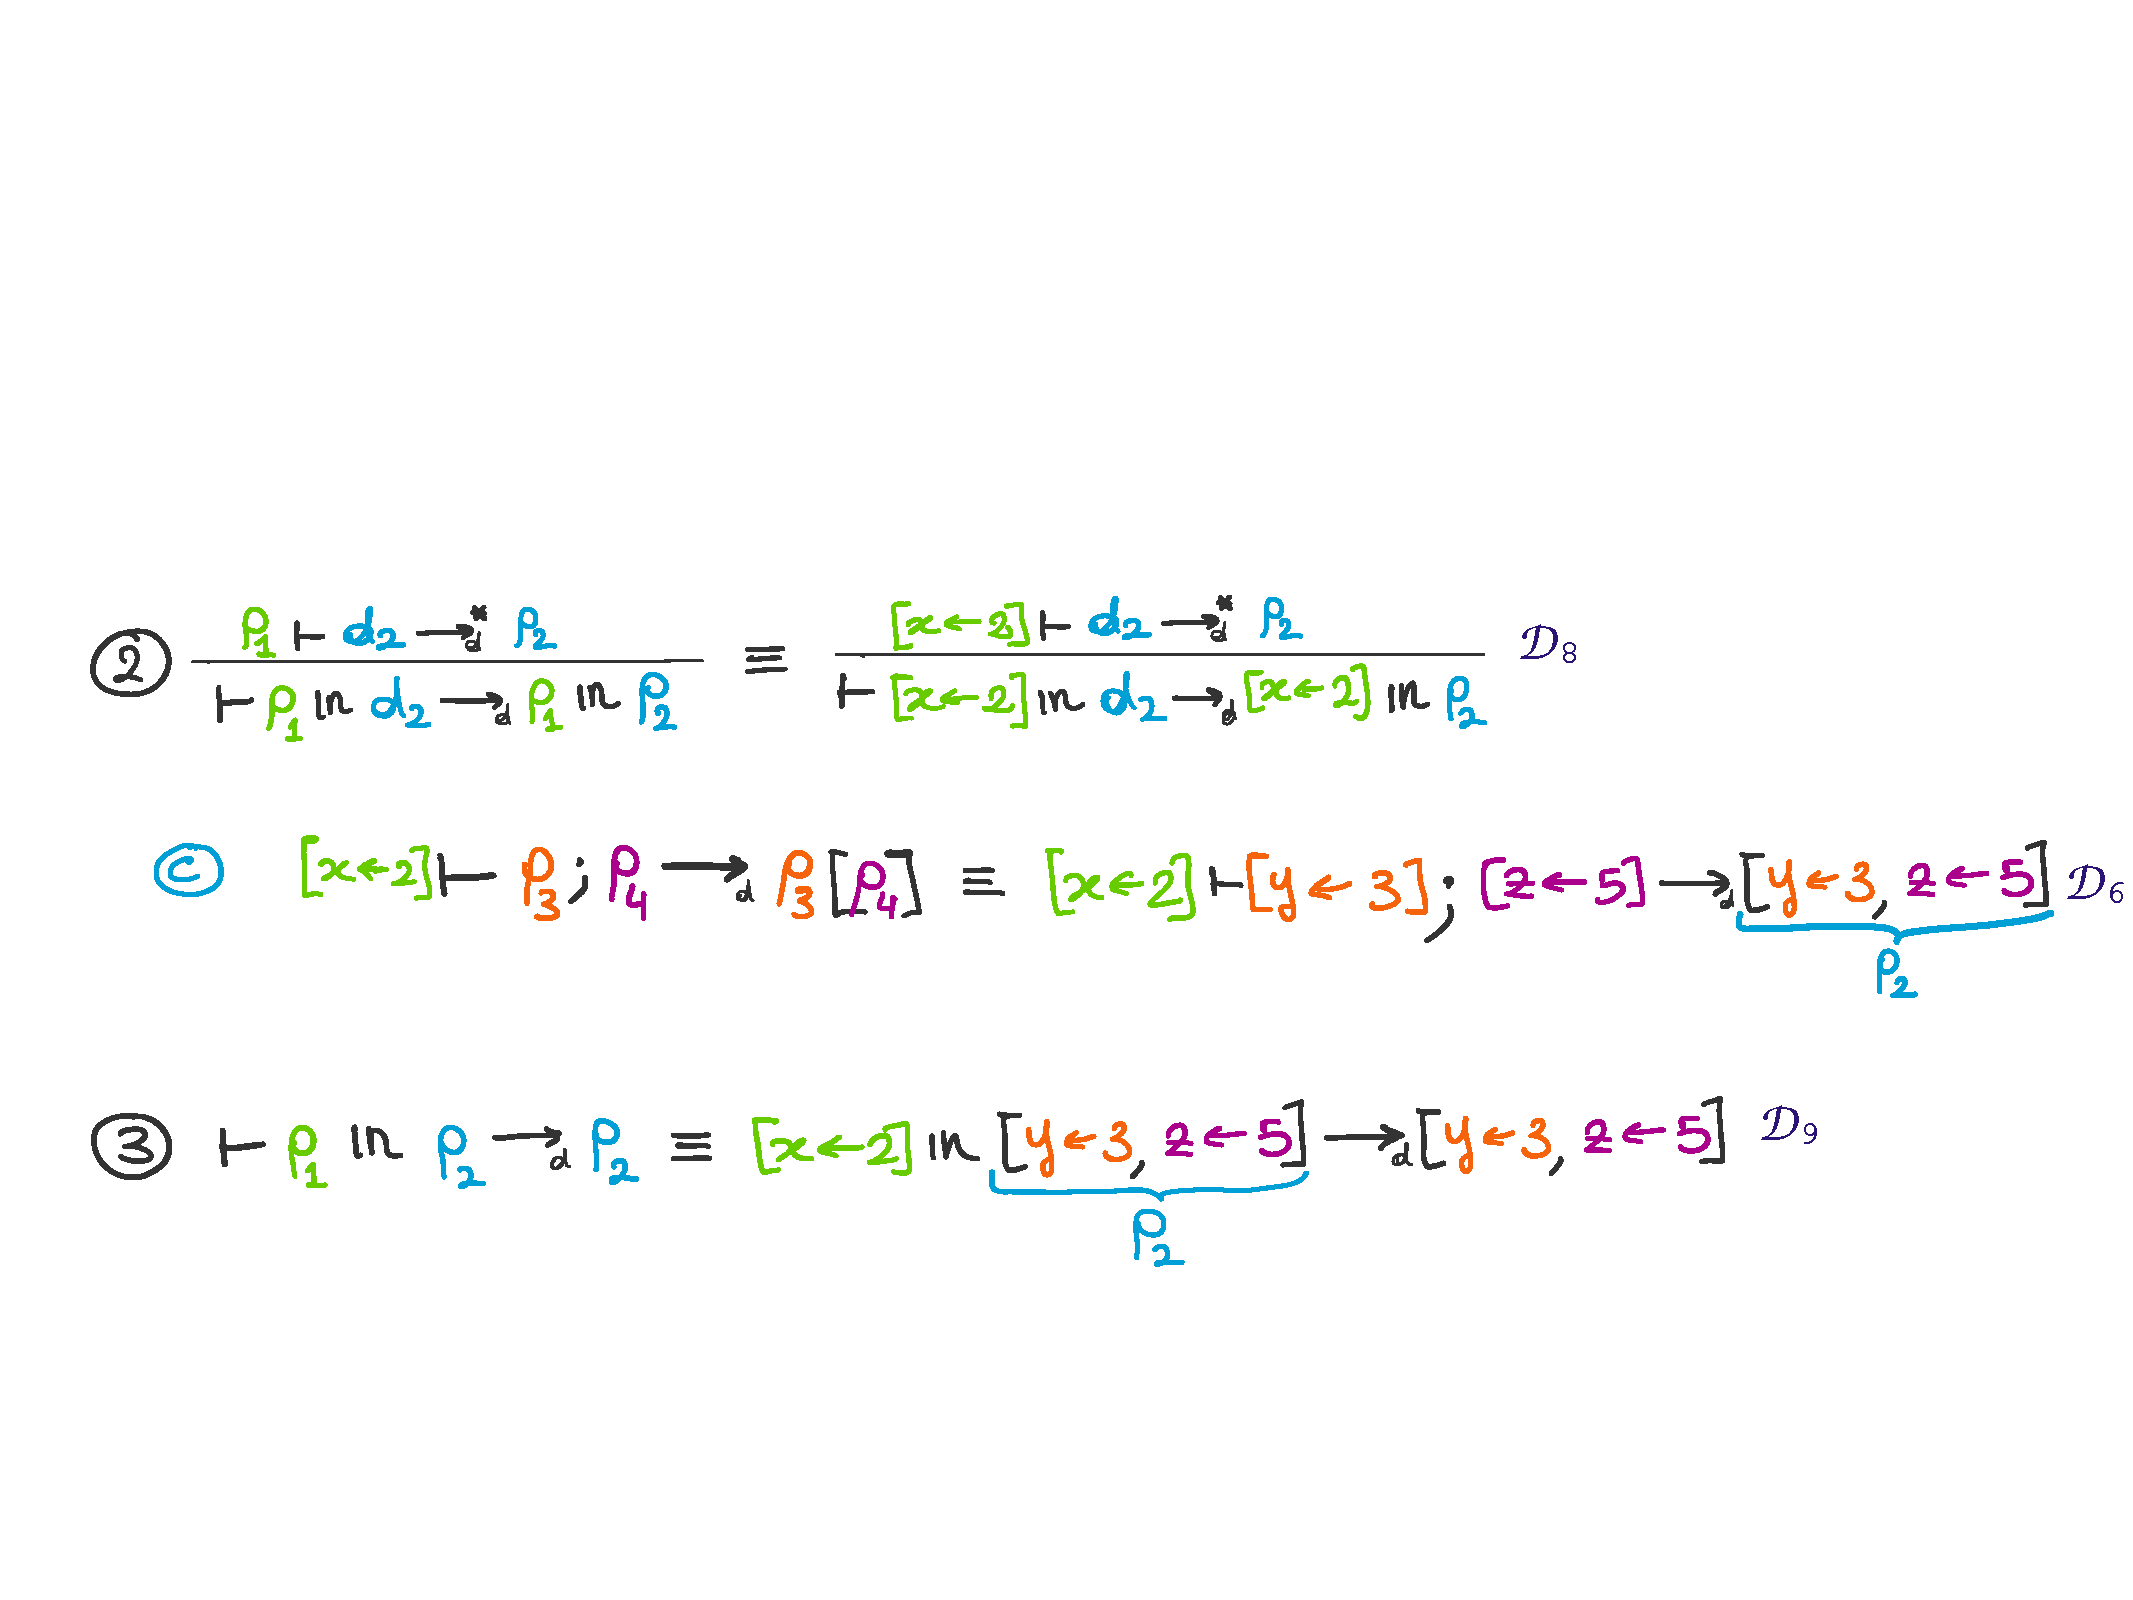
\includegraphics[width=\textwidth]{img/regola_espressione-ex7.pdf}
	\end{figure}\newpage

	\section{Comandi}
	
	\subsection{Introduzione ai concetti}
	
	Qua di seguito vengono introdotti un po' di concetti utili per il capitolo sui comandi:
	\begin{itemize}
		\item La \textcolor{Red3}{\textbf{memoria}} è un \textbf{insieme di associazioni tra locazioni e valori}. È possibile immaginarla come un \emph{array} illimitato in cui ogni indice rappresenta una locazione e il valore corrispondente è il contenuto della locazione.\newline
		Per \textbf{trasformare lo stato della memoria}, è necessario un meccanismo presente nei linguaggi imperativi chiamato \textbf{assegnamento}. Esso consente di modificare il contenuto della memoria.
		
		\item Le \textcolor{Red3}{\textbf{variabili}} sono \textbf{identificatori associati a locazioni}, le quali a loro volta, nella memoria, sono associate a valori che possono cambiare durante l'esecuzione.\newline
		La loro introduzione è stata necessaria poiché un programma sarebbe dipendente dall'implementazione fisica lavorando con gli indirizzi di memoria.
		
		\item I \textcolor{Red3}{\textbf{comandi}} contengono \textbf{costrutti necessari per la composizione e il controllo del flusso di esecuzione}.
	\end{itemize}\newpage

	\subsection{Memoria e locazioni}
	
	Ogni nuovo oggetto può usufruire di una nuova locazione. Questo perché viene reso possibile che una \textbf{variabile possa avere indirizzi differenti in differenti momenti dell'esecuzione}, oppure che una \textbf{variabile posso avere indirizzi differenti in diversi punti del programma}. Nel caso in cui, nello stesso momento, due nomi di variabili possono essere usati per accedere alla stessa locazione, allora questi sono detti \textbf{alias}.\newline
	Quindi, la \textbf{locazione associata ad una variabile astrae l'indirizzo di memoria in cui il valore della variabile si trova}.\newline
	
	\noindent
	Lo \textbf{stato di ogni macchina viene rappresentato attraverso la sua memoria}, ovvero attraverso l'insieme di associazioni tra locazioni (riferibili mediante variabili) e valori memorizzabili.
	
	Quindi, la \textbf{memoria è lo strumento utilizzato per tenere traccia dell'evoluzione dei valori delle variabili}, attraverso la descrizione dei valori che stanno nelle locazioni associate alle variabili.\:\newline
	
	\noindent	
	\begin{boxdef}
		\textbf{La} \textcolor{Red3}{\textbf{locazione/indirizzo}} \textbf{è un contenitore per i valori che può essere inutilizzata, indefinita o definita.}
	\end{boxdef}\:\newline
	
	\noindent
	\begin{boxdef}
		\textbf{La} \textcolor{Red3}{\textbf{memoria}} \textbf{è una collezione di associazioni con gli identificatori, che vengono aggiornate dinamicamente, fotografate in un istante.}
	\end{boxdef}\:\newline

	\noindent
	Il \textbf{tempo di vita} di una \textbf{locazione} è determinato dallo \emph{scope} (visibilità) della dichiarazione. Invece, il modo con cui si \textbf{rilascia la locazione determina la reversibilità dei cambiamenti}:
	\begin{itemize}
		\item Se il rilascio è \textbf{implicito} (automatico) il cambiamento è reversibile.
		
		\item Se il rilascio è \textbf{esplicito} (allocazione dinamica) allora anche questi cambiamenti diventano non reversibili.
	\end{itemize}\newpage

	\subsection{Nuova grammatica per le dichiarazioni: aggiornamento della sintassi}
	
	Con l'introduzione della memoria, è necessario aggiungere una dichiarazione alla grammatica delle dichiarazioni, così che consenta di definite un nuovo oggetto sintattico:
	\begin{equation*}
		\begin{array}{rrll}
			\mathcal{D}^{V}: \mathrm{<Dec>} \: \mathrm{D} \: \rightarrow & \mathrm{nil} & | & \mathrm{const} \:\: \mathrm{I}:\tau = \mathrm{e} \:\: | \\
			& \mathrm{var} \:\: \mathrm{I}:\tau = \mathrm{e} & | & \\
			& \mathrm{D} \:\: \mathrm{in} \:\: \mathrm{D} & | & D \:\: ; \:\: \mathrm{D} \:\: | \:\: \rho
		\end{array}
	\end{equation*}

	\noindent
	Dove $\mathcal{D}^{V}$ è l'\textbf{insieme di dichiarazioni con variabili}, che nella semantica costituiscono l'insieme delle configurazioni del sistema di transizione.
	
	La nuova grammatica definisce un identificatore $x$ come una variabile di tipo $\tau$ ed inizializzata al valore denotato dall'espressione $e$.\newline
	
	\noindent
	Le \textbf{funzioni definite sulla sintassi}, ovvero $DI$ (identificatori definiti, paragrafo~\ref{identificatori definiti}) e $FI$ (identificatori liberi, paragrafo~\ref{identificatori liberi}), vengono aggiornate (in rosso gli aggiornamenti) nel seguente modo (le spiegazioni si trovano nei paragrafi indicati):
	\begin{equation*}
		\begin{array}{lll}
			DI\left(\mathsf{nil}\right) & = & \emptyset \\
			DI\left(\mathbf{const} \: \mathsf{x}: \tau = \mathrm{e}\right) & = & \textcolor{Red3}{DI\left(\mathbf{var} \: \mathsf{x}: \tau = \mathrm{e}\right)} = \left\{x\right\} \\
			DI\left(d_{0} ; d_{1}\right) & = & DI\left(d_{0}\right) \cup DI\left(d_{1}\right) \\
			DI\left(d_{0} \: \mathsf{in} \: d_{1}\right) & = & DI\left(d_{1}\right) \\
			DI\left(\rho\right) & = & I, \hspace{1em} \text{con } \rho : I \\
			\\
			FI\left(\mathsf{nil}\right) & = & \emptyset \\
			FI\left(\mathbf{const} \: \mathsf{x}: \tau = \mathrm{e}\right) & = & \textcolor{Red3}{FI\left(\mathbf{var} \: \mathsf{x}: \tau = \mathrm{e}\right)} = FI\left(\mathrm{e}\right) \\
			FI\left(d_{0} ; d_{1}\right) & = & FI\left(d_{0} \: \mathsf{in} \: d_{1}\right) = FI\left(d_{0}\right) \cup \left(FI\left(d_{1}\right) \setminus DI\left(d_{0}\right)\right) \\
			FI\left(\rho\right) & = & \emptyset
		\end{array}
	\end{equation*}\newpage

	\subsection{Le variabili}
	
	Le \textcolor{Red3}{\textbf{variabili}} sono caratterizzate da vari aspetti, i quali sono \textbf{\underline{in comune} con gli identificatori costanti}:
	\begin{itemize}
		\item \textbf{Nome/identificatore}, rappresenta la sequenza di caratteri utilizzati per \textbf{riferirsi all'oggetto denotato};
		
		\item \textbf{Tipo}, rappresenta l'\textbf{insieme dei valori riferibili dalla variabile}, ovvero quei valori memorizzabili nella locazione legata all'identificatore, e dalle \textbf{operazioni possibili su questi valori};
		
		\item \textbf{Valore}, rappresenta l'\textbf{oggetto memorizzato nella locazione associato all'identificatore}. Ovviamente deve essere tra quelli identificati dal tipo della variabile.
	\end{itemize}
	Invece, le \textbf{caratteristiche \underline{differenti} da un identificatore costante}, e quindi proprie delle variabili, sono:
	\begin{itemize}
		\item \textbf{Indirizzo/locazione}, rappresenta l'\textbf{astrazione della cella di memoria} in cui il valore associato viene memorizzato. È l'oggetto denotabile legato all'identificatore della variabile;
		
		\item \textbf{Scope}, rappresenta il \textbf{range dei comandi a cui la variabile è visibile}, ovvero dove è visibile la sua dichiarazione;
		
		\item \textbf{Tempo di vita}, rappresenta il \textbf{tempo in cui il \emph{binding} con la locazione è attivo}.
	\end{itemize}\newpage
	
	\subsubsection{Semantica statica per le variabili e nuove regole}
	
	Viene introdotto un nuovo tipo così da \textbf{distinguere gli identificatori variabili e costanti}. Si definisce il tipo $\mathsf{\tau loc}$ utilizzato per gli identificatori variabili di tipo $\tau$:
	\begin{equation*}
		\begin{array}{rll}
			\tau \in \mathrm{DTyp} & = & \left\{\mathsf{int}, \mathsf{bool}, \bot\right\} \\
			\mathsf{\tau loc} \in \mathrm{DTypLoc} & = & \left\{\mathsf{intloc}, \mathsf{boolloc}\right\} \\
			\mathrm{Typ} & = & \mathrm{DTyp} \cup \mathrm{DTypLoc}
		\end{array}
	\end{equation*}
	Le regole di semantica statica date nel paragrafo~\ref{semantica statica delle espressioni} sono esattamente le stesse. Tuttavia, viene \textbf{aggiunta la regola per la nuova dichiarazione}:
	\begin{equation*}
		\mathcal{D}\mathrm{s}_{6} : \dfrac{
			\Delta\vdash \:\: \mathrm{e} : \textcolor{Red3}{\tau}
		}{
			\Delta\vdash \:\: \mathbf{var} \:\: \mathrm{x}:\textcolor{Red3}{\tau} = \mathrm{e} : \left[\mathrm{x} \leftarrow \textcolor{Red3}{\tau} \mathrm{loc}\right]
		}
	\end{equation*}

	\noindent
 	Dato che $\tau \in \mathrm{DTyp}$, si dice che la dichiarazione è \textbf{ben formata} (come per le costanti) \textbf{se il tipo dichiarato coincide con il tipo dell'espressione usata per inizializzare}. In tal caso, l'ambiente statico ottenuto associa alla variabile $x$ il tipo $\tau \mathrm{loc}$.\newline
 	
 	\noindent
 	Per \textcolor{Green4}{\textbf{esempio}}, se viene dichiarata una variabile $x$ di tipo $int$ e viene inizializzata con il valore $3$, allora la dichiarazione è ben formata e l'ambiente statico associa ad $x$ il tipo $intloc$.\newline
 	
 	\noindent
 	Questa modifica \textbf{cambia} anche la \textbf{regola semantica statica per gli identificatori che ora possono essere di tipo variabile}:
 	\begin{equation*}
 		\mathcal{E}\mathrm{s}_{3} : \:\: \Delta \vdash_{V} \:\: \mathrm{I} : \textcolor{Red3}{\tau} \hspace{1em} \mathrm{se} \:\: \Delta\left(\mathrm{I}\right) \in \left\{\textcolor{Red3}{\tau}, \textcolor{Red3}{\tau}\mathrm{loc}\right\}, \: \mathrm{I} \in \mathrm{V}
 	\end{equation*}\newpage
 
 	\subsection{Memoria e locazioni in $IMP$}
 	
 	Le \textbf{locazioni} sono modellate come un insieme finito ma illimitato di elementi che rappresentano celle di memoria:
 	\begin{boxdef}
 		\textbf{L'insieme} $Loc$ \textbf{è una collezione illimitata di locazioni:}
 		\begin{equation*}
 			L \subseteq Loc \hspace{2em} New\left(L\right) \in Loc \setminus L
 		\end{equation*}
 	\end{boxdef}
 	
 	\noindent
 	Dove la funzione $New$ \textbf{prende un insieme di locazioni già utilizzate e ne genera una nuova da utilizzare}.\newline
 	
 	\noindent
 	Siano $MVal$ i valori memorizzabili, ovvero quelli che possono essere associati ad una locazione. Si definiscono come $MVal$ i valori interi e booleani:
 	\begin{equation*}
 		MVal = \mathcal{N} \cup \mathcal{B}
 	\end{equation*}
 	Allora è possibile definire formalmente il concetto di memoria.
 	
 	\begin{boxdef}
 		Una \textcolor{Red3}{\textbf{memoria formalmente}} \textbf{è un elemento dello spazio di funzioni} $Mem$ definito da:
 		\begin{equation*}
 			Mem = \bigcup_{L\subseteq_{f} Loc} Mem_{L}
 		\end{equation*}
 		\textbf{Dove}:
 		\begin{equation*}
 			Mem_{L} : L \longrightarrow MVal
 		\end{equation*}
 		\textbf{Ha una metavariabile} $\sigma$ \textbf{e} $MVal$ \textbf{sono i valori memorizzabili.}
 	\end{boxdef}
 
 	\noindent
 	Dove $Loc_{\tau}$ è l'unione degli insiemi $Loc$ delle locazioni che possono memorizzare valori di tipo $\tau$.\newline
 	
 	\noindent
 	Si considerino due memoria $\sigma$, $\sigma' \in Mem$ dove $\sigma: L$ (sigma è compatibile con $L$) e $\sigma' : L' \left(L, L' \subseteq Loc\right)$, ovvero $\sigma$ è definito sulle locazioni in $L$ e $\sigma'$ è definito sull'insieme di locazioni.
 	
 	L'\textbf{aggiornamento della memoria} $\sigma$ mediante la memoria $\sigma'$ è la memoria $\sigma''\in Mem$, denotato con $\sigma\left[\sigma'\right]$ e definito come:
 	\begin{equation*}
 		\sigma''\left(l\right) = \begin{cases}
 			\sigma'\left(l\right)	& \text{se } l \in L' \\
 			\sigma\left(l\right)	& \text{altrimenti}
 		\end{cases}
 	\end{equation*}
 	In altre parole, \textbf{la memoria che aggiorna ha la precedenza, tutto quello di cui questa memoria non parla rimane inalterato}.\newpage
 	
 	\subsection{Aggiungere la memoria nei sistemi di transizione e nelle regole}
 	
 	\begin{boxdef}
 		Le \textcolor{Red3}{\textbf{espressioni}} hanno il seguente \textbf{sistema di transizione}:
 		\begin{equation*}
 			I^{V} = \mathcal{E}^{V} \times Mem, \hspace{1em} T^{V} = \left(\mathcal{N} \cup \mathcal{B}\right) \times Mem
 		\end{equation*}
 	\end{boxdef}
 	
 	\noindent
 	Le regole assumono la seguente struttura:
	\begin{equation*}
		\mathcal{E}_{\mathrm{i}}: \:\: \rho \:\: \vdash_{\Delta} \:\: \left\langle \mathrm{e},\textcolor{Red3}{\sigma} \right\rangle \rightarrow_{\mathrm{e}} \left\langle \mathrm{e}', \textcolor{Red3}{\sigma} \right\rangle
	\end{equation*}
 
 	\noindent
 	L'unica regola che \textbf{cambia} è quella di \textbf{valutazione degli identificatori}, la quale deve considerare il caso in cui l'identificatore sia una variabile:
 	\begin{equation*}
 		\mathcal{E}_{2} : \:\: \rho\vdash_{\Delta} \:\: \left\langle \mathrm{I}, \sigma \right\rangle \rightarrow_{\mathrm{e}} \left\langle \mathrm{n}, \sigma \right\rangle \:\: \mathrm{se} \:\: \rho\left(\mathrm{I}\right) = \mathrm{n} \:\:\: \mathrm{o} \:\:\: \overbrace{\left(\rho\left(\mathrm{I}\right) = \mathrm{l} \: \mathrm{e} \: \sigma\left(\mathrm{l}\right) = \mathrm{n}\right)}
 	\end{equation*}
 	
 	\noindent
 	Per le \textbf{altre regole}, basta aggiungere la memoria nella regola. Tuttavia, si osserva che tale memoria non può essere trasformata dalla valutazione, la quale accede in memoria sempre e solo in lettura.\newline
 	
 	\noindent
 	\begin{boxdef}
 		Le \textcolor{Red3}{\textbf{dichiarazioni}} hanno il seguente \textbf{sistema di transizione}:
 		\begin{equation*}
 			I^{V} = \mathcal{D}^{V} \times Mem, \hspace{1em} T^{V} = Env \times Mem
 		\end{equation*}
 	\end{boxdef}
 	
 	\noindent
 	Le regole assumono la seguente struttura:
	\begin{equation*}
		\mathcal{D}_{\mathrm{i}} : \:\: \rho \:\: \vdash_{\Delta} \:\: \left\langle \mathrm{d}, \textcolor{Red3}{\sigma} \right\rangle \rightarrow_{\mathrm{d}} \left\langle \mathrm{d}', \textcolor{Red3}{\sigma'} \right\rangle
	\end{equation*}
 	
 	\noindent
 	Dopo la transazione, la \textbf{memoria può essere diversa} poiché le dichiarazioni, \textbf{inizializzando le variabili}, \textbf{modificano la memoria}.\newpage
 	
 	\subsubsection{Regole definitive delle espressioni con variabili}
 	
 	Vengono riportate qua di seguito le regole aggiornate con la memoria:
 	\begin{itemize}
 		\item La prima regola:
 		\begin{gather*}
 			\mathcal{E}_{1}: \:\: \rho \:\: \vdash_{\Delta} \:\: \left\langle \mathrm{m} \:\: \mathbf{op} \:\: \mathrm{n}, \textcolor{Red3}{\sigma} \right\rangle \rightarrow_{\mathrm{e}} \left\langle \mathrm{k}, \textcolor{Red3}{\sigma} \right\rangle \\
 			\mathrm{se} \hspace{1em} \mathrm{m} \:\: \mathrm{op} \:\: \mathrm{n} = \mathrm{k}, \hspace{1em} \mathrm{m,n} \in \mathcal{N} \hspace{1em} \mathrm{k} \in \mathcal{N} \cup \mathcal{B}
 		\end{gather*}
 		
 		\item La seconda regola:
 		\begin{gather*}
 			\mathcal{E}_{2} : \:\: \rho \:\: \vdash_{\Delta} \:\: \left\langle \mathrm{I}, \textcolor{Red3}{\sigma} \right\rangle \rightarrow_{\mathrm{e}} \left\langle \mathrm{n}, \textcolor{Red3}{\sigma} \right\rangle \\
 			\mathrm{se} \hspace{1em} \rho\left(\mathrm{I}\right) = \mathrm{n} \hspace{1em} \mathrm{o} \hspace{1em} \textcolor{Red3}{\left(\rho\left(\mathrm{I}\right) = \mathrm{l} \:\: \mathrm{e} \:\: \sigma\left(\mathrm{l}\right) = \mathrm{n}\right)}
 		\end{gather*}
 		
 		\item La terza regola:
 		\begin{equation*}
 			\mathcal{E}_{3} : \dfrac{
 				\rho \:\: \vdash_{\Delta} \:\: \left\langle \mathrm{e}, \textcolor{Red3}{\sigma} \right\rangle \rightarrow_{\mathrm{e}} \left\langle \mathrm{e}', \textcolor{Red3}{\sigma} \right\rangle
 			}{
 				\rho \:\: \vdash_{\Delta} \:\: \left\langle \mathrm{e} \:\: \mathbf{op} \:\: \mathrm{e}_{0}, \textcolor{Red3}{\sigma} \right\rangle \rightarrow_{\mathrm{e}} \left\langle \mathrm{e}' \:\: \mathbf{op} \:\: \mathrm{e}_{0}, \textcolor{Red3}{\sigma} \right\rangle
 			}
 		\end{equation*}
 		
 		\item La quarta regola:
 		\begin{equation*}
 			\mathcal{E}_{4} : \dfrac{
 				\rho \:\: \vdash_{\Delta} \:\: \left\langle \mathrm{e}, \textcolor{Red3}{\sigma} \right\rangle \rightarrow_{\mathrm{e}} \left\langle \mathrm{e}', \textcolor{Red3}{\sigma} \right\rangle
 			}{
 				\rho \:\: \vdash_{\Delta} \:\: \left\langle \mathrm{m} \:\: \mathbf{op} \:\: \mathrm{e}, \textcolor{Red3}{\sigma} \right\rangle \rightarrow_{\mathrm{e}} \left\langle \mathrm{m} \:\: \mathbf{op} \:\: \mathrm{e}', \textcolor{Red3}{\sigma} \right\rangle
 			}
 		\end{equation*}
 		
 		\item La quinta regola:
 		\begin{gather*}
 			\mathcal{E}_{5} : \rho \:\: \vdash_{\Delta} \:\: \left\langle \mathrm{t}_{1} \:\: \mathbf{bop} \:\: \mathrm{t}_{2}, \textcolor{Red3}{\sigma} \right\rangle \rightarrow_{\mathrm{e}} \left\langle \mathrm{t}, \textcolor{Red3}{\sigma} \right\rangle \\
 			\mathrm{se} \hspace{1em} \mathrm{t}_{1} \:\: \mathrm{op} \:\: \mathrm{t}_{2} = \mathrm{t}, \hspace{1em} \mathrm{t_{1}, t_{2}, t} \in \mathcal{B}
 		\end{gather*}
 		
 		\item La terza regola aggiornata:
 		\begin{equation*}
 			\mathcal{E}_{3'} : \dfrac{
 				\rho \:\: \vdash_{\Delta} \:\: \left\langle \mathrm{e}, \textcolor{Red3}{\sigma} \right\rangle \rightarrow_{\mathrm{e}} \left\langle \mathrm{e}', \textcolor{Red3}{\sigma} \right\rangle
 			}{
 				\rho \:\: \vdash_{\Delta} \:\: \left\langle \mathrm{e} \:\: \mathbf{bop} \:\: \mathrm{e}_{0}, \textcolor{Red3}{\sigma} \right\rangle \rightarrow_{\mathrm{e}} \left\langle \mathrm{e}' \:\: \mathbf{bop} \:\: \mathrm{e}_{0}, \textcolor{Red3}{\sigma} \right\rangle
 			}
 		\end{equation*}
 		
 		\item La sesta regola:
 		\begin{equation*}
 			\mathcal{E}_{6} : \dfrac{
 				\rho \:\: \vdash_{\Delta} \:\: \left\langle \mathrm{e}, \textcolor{Red3}{\sigma} \right\rangle \rightarrow_{\mathrm{e}} \left\langle \mathrm{e}', \textcolor{Red3}{\sigma} \right\rangle
 			}{
 				\rho \:\: \vdash_{\Delta} \:\: \left\langle \mathrm{t} \:\: \mathbf{bop} \:\: \mathrm{e}, \textcolor{Red3}{\sigma} \right\rangle \rightarrow_{\mathrm{e}} \left\langle \mathrm{t} \:\: \mathbf{bop} \:\: \mathrm{e}', \textcolor{Red3}{\sigma} \right\rangle
 			}
 		\end{equation*}
 		
 		\item La settima regola:
 		\begin{gather*}
 			\mathcal{E}_{7} : \:\: \rho \:\: \vdash_{\Delta} \:\: \left\langle \mathbf{not} \:\: \mathrm{t}_{1}, \textcolor{Red3}{\sigma} \right\rangle \rightarrow_{\mathrm{e}} \left\langle \mathrm{t}, \textcolor{Red3}{\sigma} \right\rangle \\
 			\mathrm{se} \hspace{1em} \mathrm{not} \:\: \mathrm{t}_{1} = \mathrm{t}, \hspace{1em} \mathrm{t}_{1} \in \mathcal{B}
 		\end{gather*}
 		
 		\item L'ottava regola:
 		\begin{equation*}
 			\mathcal{E}_{8} : \dfrac{
 				\rho \:\: \vdash_{\Delta} \:\: \left\langle \mathrm{e}, \textcolor{Red3}{\sigma} \right\rangle \rightarrow_{\mathrm{e}} \left\langle \mathrm{e}', \textcolor{Red3}{\sigma} \right\rangle
 			}{
 				\rho \:\: \vdash_{\Delta} \:\: \left\langle \mathbf{not} \:\: \mathrm{e}, \textcolor{Red3}{\sigma} \right\rangle \rightarrow_{\mathrm{e}} \left\langle \mathbf{not} \:\: \mathrm{e}', \textcolor{Red3}{\sigma} \right\rangle
 			}
 		\end{equation*}
 	\end{itemize}\newpage
 	
 	\subsubsection{Regole definitive delle espressioni con chiusura transitiva}
 	
 	Un sistema di regole equivalente al paragrafo precedente ma che utilizza la chiusura transitiva nelle premesse:
 	\begin{itemize} 		
 		\item La seconda regola:
 		\begin{gather*}
 			\textcolor{Red3}{\mathcal{E}_{2}} : \:\: \rho \:\: \vdash_{\Delta} \:\: \left\langle \mathrm{I}, \textcolor{Red3}{\sigma} \right\rangle \rightarrow_{\mathrm{e}} \left\langle \mathrm{n}, \textcolor{Red3}{\sigma} \right\rangle \\
 			\mathrm{se} \:\: \rho \left(\mathrm{I}\right) = \mathrm{n} \:\: \mathrm{o} \:\: \textcolor{Red3}{\left(\rho\left(\mathrm{I}\right) = \mathrm{l} \:\: \mathrm{e} \:\: \sigma\left(\mathrm{l}\right) = \mathrm{n}\right)}
 		\end{gather*}
 		
 		\item La terza e la quarta regola:
 		\begin{equation*}
 			\mathcal{E}_{3\text{-}4} : \dfrac{
 				\rho \:\: \vdash_{\Delta} \:\: \left\langle \mathrm{e}, \textcolor{Red3}{\sigma} \right\rangle \rightarrow^{*}_{\mathrm{e}} \left\langle \mathrm{m}, \textcolor{Red3}{\sigma} \right\rangle
 			}{
 				\rho \:\: \vdash_{\Delta} \:\: \left\langle \mathrm{e} \:\: \mathbf{op} \:\: \mathrm{e}_{0}, \textcolor{Red3}{\sigma} \right\rangle \rightarrow_{\mathrm{e}} \left\langle \mathrm{k} \:\: \mathbf{op} \:\: \mathrm{e}_{0}, \textcolor{Red3}{\sigma} \right\rangle
 			}
 		\end{equation*}
 		
 		\item La quarta e la prima regola:
 		\begin{gather*}
 			\mathcal{E}_{4\text{-}1} : \dfrac{
 				\rho \:\: \vdash_{\Delta} \:\: \left\langle \mathrm{e}, \textcolor{Red3}{\sigma} \right\rangle \rightarrow^{*}_{\mathrm{e}} \left\langle \mathrm{n}, \textcolor{Red3}{\sigma} \right\rangle
 			}{
 				\rho \:\: \vdash_{\Delta} \:\: \left\langle \mathrm{m} \:\: \mathbf{op} \:\: \mathrm{e}, \textcolor{Red3}{\sigma} \right\rangle \rightarrow_{\mathrm{e}} \left\langle \mathrm{k}, \textcolor{Red3}{\sigma} \right\rangle
 			} \\
 			\\
 			\mathrm{m} \:\: \mathrm{op} \:\: \mathrm{n} = \mathrm{k} \hspace{2em} \mathrm{m,n} \in \mathcal{N} \hspace{2em} \mathrm{k} \in \mathcal{N}
 		\end{gather*}
 		
 		\item La terza regola aggiornata e la sesta:
 		\begin{equation*}
 			\mathcal{E}_{3'\text{-}6} : \dfrac{
 				\rho \:\: \vdash_{\Delta} \:\: \left\langle \mathrm{e}, \textcolor{Red3}{\sigma} \right\rangle \rightarrow_{\mathrm{e}}^{*} \left\langle \mathrm{t}, \textcolor{Red3}{\sigma} \right\rangle
 			}{
 				\rho \:\: \vdash_{\Delta} \:\: \left\langle \mathrm{e} \:\: \mathbf{bop} \:\: \mathrm{e}_{0}, \textcolor{Red3}{\sigma} \right\rangle \rightarrow_{\mathrm{e}} \left\langle \mathrm{t} \:\: \mathbf{bop} \:\: \mathrm{e}_{0}, \textcolor{Red3}{\sigma} \right\rangle
 			}
 		\end{equation*}
 		
 		\item La sesta e la quinta regola:
 		\begin{gather*}
 			\mathcal{E}_{6\text{-}5} : \dfrac{
 				\rho \:\: \vdash_{\Delta} \:\: \left\langle \mathrm{e}, \textcolor{Red3}{\sigma} \right\rangle \rightarrow_{\mathrm{e}}^{*} \left\langle \mathrm{t}_{2}, \textcolor{Red3}{\sigma} \right\rangle
 			}{
 				\rho \:\: \vdash_{\Delta} \:\: \left\langle \mathrm{t}_{1} \:\: \mathbf{bop} \:\: \mathrm{e}, \textcolor{Red3}{\sigma} \right\rangle \rightarrow_{\mathrm{e}} \left\langle \mathrm{t}, \textcolor{Red3}{\sigma} \right\rangle
 			} \\
 			\\
 			\mathrm{se} \hspace{1em} \mathrm{t}_{1} \:\: \mathrm{op} \:\: \mathrm{t}_{2} = \mathrm{t}, \hspace{2em} \mathrm{t_{1}, t_{2}, t} \in \mathcal{B}
 		\end{gather*}
 		
 		\item L'ottava e la settima regola:
 		\begin{gather*}
 			\mathcal{E}_{8\text{-}7} : \dfrac{
 				\rho \:\: \vdash_{\Delta} \:\: \left\langle \mathrm{e}, \textcolor{Red3}{\sigma} \right\rangle \rightarrow_{\mathrm{e}}^{*} \left\langle \mathrm{t}_{1}, \textcolor{Red3}{\sigma} \right\rangle
 			}{
 				\rho \:\: \vdash_{\Delta} \:\: \left\langle \mathbf{not} \:\: \mathrm{e}, \textcolor{Red3}{\sigma} \right\rangle \rightarrow_{\mathrm{e}} \left\langle \mathrm{t}, \textcolor{Red3}{\sigma} \right\rangle
 			} \\
 			\\
 			\mathrm{se} \hspace{1em} \mathrm{not} \:\: \mathrm{t}_{1} = \mathrm{t}, \hspace{2em} \mathrm{t}_{1} \in \mathcal{B}
 		\end{gather*}
 	\end{itemize}\newpage
 	
 	\subsubsection{Espressioni: valutazione ed equivalenza con variabili}
 	
 	La \textbf{funzione di valutazione} non cambia concettualmente ma solo formalmente, in quanto è necessario considerare anche le memorie.
 	
 	\begin{boxdef}
 		La \textcolor{Red3}{\textbf{valutazione delle espressioni con variabili}} è la seguente. \textbf{La valutazione è una funzione:}
 		\begin{equation*}
 			Eval: \mathcal{E}^{V} \times Mem \longrightarrow \mathbb{N} \cup \mathbb{B} \times Mem
 		\end{equation*}
 		\textbf{Che descrive il comportamento dinamico delle espressioni restituendo il valore in cui esse sono valutate (insieme alla memoria):}
 		\begin{equation*}
 			Eval\left(\langle e, \rho \rangle\right) = k \iff \langle e,\rho \rangle \longrightarrow^{*} \langle k,\rho \rangle
 		\end{equation*}
 	\end{boxdef}\:\newline
 
 	\noindent
 	L'\textbf{equivalenza} cambia poiché il valore risultante dipende potenzialmente dalla memoria da cui si parte. Allora c'è equivalenza se e solo se il valore risultante è lo stesso per tutte le possibili memorie iniziali:
 	
 	\begin{boxdef}
 		\textbf{L'}\textcolor{Red3}{\textbf{equivalenza di espressioni con variabili}} \textbf{è una relazione:}
 		\begin{equation*}
 			\equiv \subseteq \mathcal{E}^{V} \times \mathcal{E}^{V}
 		\end{equation*}
 		\textbf{Definita come segue:}
 		\begin{equation*}
 			e_{0} \equiv e_{1} \iff \forall \sigma. \: Eval\left(\langle e_{0},\sigma \rangle\right) = Eval\left( \langle e_{1},\sigma \rangle \right)
 		\end{equation*}
 	\end{boxdef}\newpage
 	
 	\subsubsection{Semantica dinamica per le variabili e regole delle dichiarazioni con variabili}
 	
 	Per la semantica dinamica, vengono introdotte \textbf{due nuove regole necessarie per la dichiarazione}:
 	\begin{itemize}
 		\item La prima regola:
 		\begin{equation*}
 			\mathcal{D}_{1}: \:\: \vdash \:\: \left\langle \mathbf{nil}, \sigma \right\rangle \rightarrow_{\mathrm{d}} \left\langle \emptyset, \sigma \right\rangle
 		\end{equation*}
 	
 		\item La seconda regola:
 		\begin{equation*}
 			\mathcal{D}_{2} : \:\: \rho \:\: \vdash_{\Delta} \:\: \left\langle \mathbf{const} \:\: \mathrm{x} : \tau = \mathrm{k}, \sigma \right\rangle \rightarrow_{\mathrm{d}} \left\langle \left[ \mathrm{x} \leftarrow \mathrm{k} \right], \sigma \right\rangle
 		\end{equation*}
 	
 		\item La terza regola:
 		\begin{equation*}
 			\mathcal{D}_{3} : \dfrac{
 				\rho \:\: \vdash_{\Delta} \:\: \left\langle \mathrm{e}, \sigma \right\rangle \rightarrow_{\mathrm{e}} \left\langle \mathrm{e}', \sigma \right\rangle
 			}{
 				\rho \:\: \vdash_{\Delta} \:\: \left\langle \mathbf{const} \:\: \mathrm{x}:\tau = \mathrm{e}, \sigma \right\rangle \rightarrow_{\mathrm{d}} \left\langle \mathbf{const} \:\: \mathrm{x}:\tau = \mathrm{e}', \sigma \right\rangle
 			}
 		\end{equation*}
 	
 		\item La quarta regola:
 		\begin{equation*}
 			\mathcal{D}_{4} : \dfrac{
 				\rho \:\: \vdash_{\Delta} \:\: \left\langle \mathrm{d}, \sigma \right\rangle \rightarrow_{\mathrm{d}} \left\langle \mathrm{d}', \sigma' \right\rangle
 			}{
 				\rho \:\: \vdash_{\Delta} \:\: \left\langle \mathrm{d} \: \mathbf{;} \: \mathrm{d}_{1}, \sigma \right\rangle \rightarrow_{\mathrm{d}} \left\langle \mathrm{d}' \: \mathbf{;} \: \mathrm{d}_{1}, \sigma' \right\rangle
 			}
 		\end{equation*}
 		
 		\item La quinta regola:
 		\begin{equation*}
 			\mathcal{D}_{5} : \dfrac{
 				\rho\left[\rho_{0}\right] \:\: \vdash_{\Delta\left[\Delta_{0}\right]} \:\: \left\langle \mathrm{d}_{1}, \sigma \right\rangle \rightarrow_{\mathrm{d}} \left\langle \mathrm{d}_{1}', \sigma' \right\rangle
 			}{
 				\rho \:\: \vdash_{\Delta} \:\: \left\langle \rho_{0} \: \mathbf{;} \: \mathrm{d}_{1}, \sigma \right\rangle \rightarrow_{\mathrm{d}} \left\langle \rho_{0} \: \mathbf{;} \: \mathrm{d}_{1}', \sigma' \right\rangle
 			}
 		\end{equation*}
 		
 		\item La sesta regola:
 		\begin{equation*}
 			\mathcal{D}_{6} : \:\: \rho \:\: \vdash_{\Delta} \:\: \left\langle \rho_{0} \: \mathbf{;} \: \rho_{1}, \sigma \right\rangle \rightarrow_{\mathrm{d}} \left\langle \rho_{0} \left[\rho_{1}\right], \sigma \right\rangle
 		\end{equation*}
 	
 		\item La settima regola:
 		\begin{equation*}
 			\mathcal{D}_{7} : \dfrac{
 				\rho \:\: \vdash_{\Delta} \:\: \left\langle \mathrm{d}, \sigma \right\rangle \rightarrow_{\mathrm{d}} \left\langle \mathrm{d}', \sigma' \right\rangle
 			}{
 				\rho \:\: \vdash_{\Delta} \:\: \left\langle \mathrm{d} \:\: \mathbf{in} \:\: \mathrm{d}_{1}, \sigma \right\rangle \rightarrow_{\mathrm{d}} \left\langle \mathrm{d}' \:\: \mathbf{in} \:\: \mathrm{d}_{1}, \sigma' \right\rangle
 			}
 		\end{equation*}
 	
 		\item L'ottava regola:
 		\begin{equation*}
 			\mathcal{D}_{8} : \dfrac{
 				\rho\left[\rho_{0}\right] \:\: \vdash_{\Delta\left[\Delta_{0}\right]} \:\: \left\langle \mathrm{d}_{1}, \sigma \right\rangle \rightarrow_{\mathrm{d}} \left\langle \mathrm{d}_{1}', \sigma' \right\rangle
 			}{
 				\rho \:\: \vdash_{\Delta} \:\: \left\langle \rho_{0} \:\: \mathbf{in} \:\: \mathrm{d}_{1}, \sigma \right\rangle \rightarrow_{\mathrm{d}} \left\langle \rho_{0} \:\: \mathbf{in} \:\: \mathrm{d}_{1}', \sigma' \right\rangle
 			}
 		\end{equation*}
 	
 		\item La nona regola:
 		\begin{equation*}
 			\mathcal{D}_{9} : \:\: \rho \:\: \vdash_{\Delta} \:\: \left\langle \rho_{0} \:\: \mathbf{in} \:\: \rho_{1}, \sigma \right\rangle \rightarrow_{\mathrm{d}} \left\langle \rho_{1}, \sigma \right\rangle
 		\end{equation*}\newpage
 	
 		\item La decima regola viene utilizzata per inizializzare una variabile. Una volta che l'espressione è stata valutata ad un valore costante $k$, allora è possibile allocare spazio per la nuova variabile. In particolare, si prende una nuova locazione $I$ di tipo $\tau$. La configurazione generata consiste nella coppia composta:
 		\begin{itemize}
 			\item Dall'ambiente dinamico che associa all'identificatore la nuova locazione $I$;
 			\item Dalla memoria iniziale aggiornata con l'associazione $I$ e il valore $k$.
 		\end{itemize}
 		\begin{gather*}
 			\mathcal{D}_{10} : \:\: \rho \:\: \vdash_{\Delta} \:\: \left\langle \mathbf{var} \:\: \mathrm{x}:\tau = \mathrm{k}, \sigma \right\rangle \rightarrow_{\mathrm{d}} \left\langle \left[x \leftarrow \mathrm{l}\right], \sigma\left[\mathrm{l} \leftarrow \mathrm{k}\right] \right\rangle \\
 			\mathrm{l} \in \mathrm{Loc}_{\tau} \:\: \text{nuova locazione}
 		\end{gather*}
 		
 		\item L'undicesima regola indica la nuova associazione rispetto a quella iniziale:
 		\begin{equation*}
 			\mathcal{D}_{11} : \dfrac{
 				\rho \:\: \vdash_{\Delta} \:\: \left\langle \mathrm{e}, \sigma \right\rangle \rightarrow_{\mathrm{e}} \left\langle \mathrm{e}', \sigma \right\rangle
 			}{
 				\rho \:\: \vdash_{\Delta} \:\: \left\langle \mathbf{var} \:\: \mathrm{x}:\tau = \mathrm{e}, \sigma \right\rangle \rightarrow_{\mathrm{d}} \left\langle \mathbf{var} \:\: \mathrm{x}:\tau = \mathrm{e}', \sigma \right\rangle
 			}
 		\end{equation*}
	\end{itemize}\newpage
 	
 	\subsubsection{Regole delle dichiarazioni con variabili e chiusura transitiva}
 	
 	Le regole che utilizzano la chiusura transitiva nelle premesse:
 	\begin{itemize}
 		\item La prima regola:
 		\begin{equation*}
 			\mathcal{D}_{1} : \:\: \vdash \:\: \left\langle \mathbf{nil}, \sigma \right\rangle \rightarrow_{\mathrm{d}} \left\langle \emptyset, \sigma \right\rangle
 		\end{equation*}
 	
 		\item La quarta e la quinta regola:
 		\begin{equation*}
 			\mathcal{D}_{4\text{-}5} : \dfrac{
 				\rho \:\: \vdash_{\Delta} \:\: \left\langle \mathrm{d}, \sigma \right\rangle \rightarrow_{\mathrm{d}}* \left\langle \rho_{0}, \sigma' \right\rangle
 			}{
 				\rho \:\: \vdash_{\Delta} \:\: \left\langle \mathrm{d} \: \mathbf{;} \: \mathrm{d}_{1}, \sigma \right\rangle \rightarrow_{\mathrm{d}} \left\langle \rho_{0} \: \mathbf{;} \: \mathrm{d}_{1}, \sigma' \right\rangle
 			}
 		\end{equation*}
 	
 		\item La quinta e la sesta regola:
 		\begin{equation*}
 			\mathcal{D}_{5\text{-}6} : \dfrac{
 				\rho\left[\rho_{0}\right] \:\: \vdash_{\Delta\left[\Delta_{0}\right]} \:\: \left\langle \mathrm{d}_{1}, \sigma \right\rangle \rightarrow_{\mathrm{d}}^{*} \left\langle \rho_{1}, \sigma' \right\rangle
 			}{
 				\rho \:\: \vdash_{\Delta} \:\: \left\langle \rho_{0} \: \mathbf{;} \: \mathrm{d}_{1}, \sigma \right\rangle \rightarrow_{\mathrm{d}} \left\langle \rho_{0}\left[\rho_{1}\right], \sigma' \right\rangle
 			}
 		\end{equation*}
 		
 		\item L'undicesima e la decima regola:
 		\begin{equation*}
 			\mathcal{D}_{11\text{-}10} : \dfrac{
 				\rho \:\: \vdash_{\Delta} \:\: \left\langle \mathrm{e}, \sigma \right\rangle \rightarrow_{\mathrm{e}}^{*} \left\langle \mathrm{k}, \sigma \right\rangle
 			}{
 				\rho \:\: \vdash_{\Delta} \:\: \left\langle \mathbf{var} \:\: \mathrm{x}:\tau = \mathrm{e}, \sigma \right\rangle \rightarrow_{\mathrm{d}} \left\langle \left[\mathrm{x} \leftarrow \mathrm{l}\right], \sigma\left[\mathrm{l} \leftarrow \mathrm{k}\right] \right\rangle
 			}
 		\end{equation*}
 	
 		\item La terza e la seconda regola:
 		\begin{equation*}
 			\mathcal{D}_{3\text{-}2} : \dfrac{
 				\rho \:\: \vdash_{\Delta} \:\: \left\langle \mathrm{e}, \sigma \right\rangle \rightarrow_{\mathrm{e}}^{*} \left\langle \mathrm{k}, \sigma \right\rangle
 			}{
 				\rho \:\: \vdash_{\Delta} \:\: \left\langle \mathbf{const} \:\: \mathrm{x}:\tau = \mathrm{e}, \sigma \right\rangle \rightarrow_{\mathrm{d}} \left\langle \left[\mathrm{x} \leftarrow \mathrm{k}\right], \sigma \right\rangle
 			}
 		\end{equation*}
 	
 		\item La settima e l'ottava regola:
 		\begin{equation*}
 			\mathcal{D}_{7\text{-}8} : \dfrac{
 				\rho \:\: \vdash_{\Delta} \:\: \left\langle \mathrm{d}, \sigma \right\rangle \rightarrow_{\mathrm{d}}^{*} \left\langle \rho_{0}, \sigma' \right\rangle
 			}{
 				\rho \:\: \vdash_{\Delta} \:\: \left\langle \mathrm{d} \:\: \mathbf{in} \:\: \mathrm{d}_{1}, \sigma \right\rangle \rightarrow_{\mathrm{d}} \left\langle \rho_{0} \:\: \mathbf{in} \:\: \mathrm{d}_{1}, \sigma' \right\rangle
 			}
 		\end{equation*}
 		
 		\item L'ottava e la nona regola:
 		\begin{equation*}
 			\mathcal{D}_{8\text{-}9} : \dfrac{
 				\rho\left[\rho_{0}\right] \:\: \vdash_{\Delta\left[\Delta_{0}\right]} \:\: \left\langle \mathrm{d}_{1}, \sigma \right\rangle \rightarrow^{*}_{\mathrm{d}} \left\langle \rho_{1}, \sigma' \right\rangle
 			}{
 				\rho \:\: \vdash_{\Delta} \:\: \left\langle \rho_{0} \:\: \mathbf{in} \:\: \mathrm{d}_{1}, \sigma \right\rangle \rightarrow_{\mathrm{d}} \left\langle \rho_{1}, \sigma' \right\rangle
 			}
 		\end{equation*}
 	\end{itemize}\newpage
 	
 	\subsubsection{Dichiarazioni: valutazione ed equivalenza con variabili}
 	
 	La funzione di \textbf{elaborazione} non cambia concettualmente, ma solo formalmente poiché è necessario considerare anche le memorie.
 	
 	\begin{boxdef}
 		L'\textcolor{Red3}{\textbf{elaborazione delle dichiarazioni con variabili}} è descritta nel seguente modo. \textbf{L'elaborazione è una funzione:}
 		\begin{equation*}
 			Elab: \mathcal{D}^{V} \times Mem \longrightarrow Env \times Mem
 		\end{equation*}
 		\textbf{Che descrive il comportamento dinamico delle dichiarazioni restituendo l'ambiente in cui esse sono elaborate:}
 		\begin{equation*}
 			Elab\left(\langle d,\sigma \rangle\right) = \langle \rho,\sigma \rangle \iff \langle d,\sigma \rangle \longrightarrow^{*} \langle \rho,\sigma' \rangle
 		\end{equation*}
 	\end{boxdef}\:\newline
 	
 	\noindent
 	L'\textbf{equivalenza} cambia concettualmente. Infatti, dato che l'ambiente risultante dipende potenzialmente dalla memoria da cui si parte, allora si avrà equivalenza se e solo se l'ambiente risultato è lo stesso per tutte le possibili memorie iniziali.
 	
 	\begin{boxdef}
 		L'\textcolor{Red3}{\textbf{equivalenza delle dichiarazioni con variabili}} è descritta nel seguente modo. \textbf{L'equivalenza di dichiarazioni con variabili è una relazione:}
 		\begin{equation*}
 			\equiv \subseteq \mathcal{D}^{V} \times \mathcal{D}^{V}
 		\end{equation*}
 		\textbf{Definita come segue:}
 		\begin{equation*}
 			d_{0} \equiv d_{1} \iff \forall \sigma. \: Elab\left(\langle d_{0},\sigma \rangle\right) = Elab\left(\langle d_{1},\sigma \rangle\right)
 		\end{equation*}
 	\end{boxdef}\newpage
 	
 	\subsection{Comandi in $IMP$}
 	
 	Si introducono i comandi nel linguaggio $IMP$ presentando la grammatica:
 	\begin{equation*}
 		\begin{array}{lll}
 			\mathbf{\mathcal{E}^{V}}  \hspace{1.5em} \mathbf{<Com>} \hspace{1.5em} \textcolor{Orange2}{\mathbf{C}} & \textcolor{Orange2}{\boldsymbol{\rightarrow}} & \mathbf{skip} \:\: \textcolor{Red3}{\boldsymbol{|}} \:\: \mathbf{I} \:\: \boldsymbol{\coloneq} \:\: \mathbf{E} \:\: \textcolor{Red3}{\boldsymbol{|}} \:\: \textcolor{Orange2}{\mathbf{C}} \:\: \boldsymbol{;} \:\: \textcolor{Orange2}{\mathbf{C}} \:\: \textcolor{Red3}{\boldsymbol{|}} \\
 			\\
 			&& \mathbf{if} \:\: \textcolor{Blue3}{\mathbf{B}} \:\: \mathbf{then} \:\: \textcolor{Orange2}{\mathbf{C}} \:\: \mathbf{else} \:\: \textcolor{Orange2}{\mathbf{C}} \:\: \textcolor{Red3}{\boldsymbol{|}} \\
 			\\
 			&& \mathbf{while} \:\: \textcolor{Blue3}{\mathbf{B}} \:\: \mathbf{do} \:\: \textcolor{Orange2}{\mathbf{C}} \:\: \textcolor{Red3}{\boldsymbol{|}} \:\: \textcolor{Purple2}{\mathbf{D}} \:\: \boldsymbol{;} \:\: \textcolor{Orange2}{\mathbf{C}}
 		\end{array}
 	\end{equation*}
 	
 	\begin{itemize}
 		\item \textsf{C} indica la \textbf{categoria sintattica dei comandi}, la quale deve operare per trasformare lo stato, cioè la memoria;
 		
 		\item \textsf{skip} è un \textbf{comando nullo} e non esegue nessuna trasformazione. È utile come elemento neutro della composizione sequenziale di comandi;
 		
 		\item \textsf{I $\coloneq$ E} è l'\textbf{assegnamento}, ovvero il comando base dei linguaggi imperativi. Indica l'assegnamento del valore di un'espressione (valore a destra, chiamato \emph{r-value}) ad un identificatore (valore a sinistra, chiamato \emph{l-value}). Quindi, rappresenta il comando primitivo per l'aggiornamento delle variabili;
 		
 		\item \textsf{;} è la \textbf{composizione sequenziale}, ovvero tutte le trasformazioni eseguite dal primo comando sono il punto di partenza per le trasformazioni che deve eseguire il secondo comando;
 		
 		\item \textsf{if B then C else C} e \textsf{while B do C}, sono due comandi di \textbf{controllo sequenza}, cioè consentono di decidere tra percorsi diversi:
 		\begin{itemize}
 			\item \textsf{if B then C else C} è il comando \textbf{condizionale} e consente di scegliere quale dei due possibili comandi eseguire, in funzione del valore (booleano) di un'espressione detta guardia (chiamato anche selettore a due vie).
 			
 			\item \textsf{while B do C} è il comando \textbf{iterativo} e consente di ripete l'esecuzione di un comando finché il valore della guardia (espressione booleana) rimane vera.
 		\end{itemize}
 		
 		\item \textsf{D ; C} è il blocco che crea un ambiente locale al comando.
 	\end{itemize}\newpage
 	
 	\subsection{Semantica}
 	
 	Per dare \textcolor{Red3}{\textbf{semantica}} ai comandi, viene introdotto il sistema di transizione. Esso ha come risultato una nuova configurazione contenete i comandi rimanenti da eseguire e la memoria risultante dalla trasformazione.\newline
 	
 	\noindent
 	\begin{boxdef}
 		Il \textcolor{Red3}{\textbf{sistema di transizione}} è identificato nel seguente modo:
 		\begin{equation*}
 			I^{V} = \mathcal{E}^{V} \times \mathrm{Mem} \cup \mathrm{Mem}, T^{V} = \mathrm{Mem}
 		\end{equation*}
 	\end{boxdef}
 	
 	\noindent
 	La \textbf{struttura generale} delle regole di transizione dei comandi è:
 	\begin{equation*}
 		c_{i} : \rho \vdash_{\Delta} \left\langle \mathsf{c}, \mathsf{\sigma} \right\rangle \longrightarrow_{c} \left\langle \mathsf{c}', \mathsf{\sigma}' \right\rangle
 	\end{equation*}
 	\begin{itemize}
 		\item $\rho$ è l'\textbf{ambiente esterno dinamico} che associa valori e/o locazioni agli identificatori;
 		
 		\item $\Delta$ è l'\textbf{ambiente statico} compatibile con $\rho$ e garantisce la correttezza dei vincoli semantici, come ad esempio i vincoli di tipo.
 		
 		\item $\left\langle \mathsf{c}, \mathsf{\sigma} \right\rangle \longrightarrow_{c} \left\langle \mathsf{c}', \mathsf{\sigma}' \right\rangle$, vengono definite regole, identificate dal pedice $c$, che a partire da una configurazione che deve eseguire $c$ a partire dalla \textbf{memoria iniziale} $\mathsf{\sigma}$, restituisce $\mathsf{c}'$ e la \textbf{memoria risultante} $\mathsf{\sigma}'$ potenzialmente trasformata.
 	\end{itemize}
 	
 	\longline
 	
 	\subsection{Assegnamento e semantica statica/dinamica}
 	
 	L'esecuzione di un \textcolor{Red3}{\textbf{assegnamento}} non restituisce un valore ma produce \textbf{trasformazioni irreversibili della memoria}. Nei linguaggi può essere rappresentato con il simbolo $=$, e in questo caso il test di uguaglianza è rappresentato con $==$, oppure con il simbolo $\coloneq$. A sinistra viene denotata una locazione (\emph{l-value}) e a destra il contenuto di una locazione (\emph{r-value}).\newline
 	
 	\noindent
 	L'\textbf{assegnamento}, nella semantica, è l'unico comando \dquotes{\textbf{atomico}}, cioè \textbf{non viene scritto in termini di altri comandi}. Tuttavia, utilizza un'altra grammatica, cioè quella delle espressioni.\newline
 	
 	\noindent
 	L'assegnamento contiene tutti \textbf{identificatori liberi}, poiché esso non può contenere dichiarazioni:
 	\begin{equation*}
 		FI\left(x \coloneq e\right) = FI\left(e\right) \cup \left\{x\right\} \hspace{2em} DI\left(x \coloneq e\right) = \emptyset
 	\end{equation*}
 	Qui di seguito vengono introdotte le \textcolor{Red3}{\textbf{regole}} della semantica statica e dinamica dell'assegnamento. La regole della semantica statica per i comandi serve solamente per verificare che il comando sia ben formato, ovvero rispetti tutti i vincoli semantici del comando. 
 	
 	Con la seguente \textbf{notazione} si indica che il comando $c$ è ben formato nell'ambiente statico $\Delta$, definito sull'insieme di identificatori $V$:
 	\begin{equation*}
 		\Delta \vdash_{V} c
 	\end{equation*}\newpage
 	
 	\noindent
 	Le \textbf{regole} sono le seguenti:
 	\begin{itemize}
 		\item L'assegnamento è ben formato se l'identificatore a sinistra del simbolo di assegnamento è un identificatore variabile e se è del tipo dell'espressione assegnata. È dunque necessario valutare il tipo $\tau$ dell'espressione nello stesso ambiente statico, il quale deve coincidere con il tipo associato dall'ambiente all'identificatore, ovvero $\tau loc$:
 		\begin{equation*}
 			\mathcal{E}\mathrm{s}_{1} : \dfrac{
 				\Delta \vdash_{\mathrm{V}} \:\: \mathrm{e} : \tau
 			}{
 				\Delta \vdash_{\mathrm{V}} \:\: \mathrm{x} \coloneq \mathrm{e}
 			} \:\: , \hspace{1em} \Delta\left(\mathrm{x}\right) = \tau \mathrm{loc}
 		\end{equation*}
 		
 		\item Per la semantica dinamica, è necessario valutare l'espressione:
 		\begin{equation*}
 			\mathcal{E}_{1} : \dfrac{
 				\rho \:\: \vdash_{\Delta} \:\: \left\langle \mathrm{e}, \sigma \right\rangle \rightarrow_{\mathrm{e}} \left\langle \mathrm{e}', \sigma \right\rangle
 			}{
 				\rho \:\: \vdash_{\Delta} \:\: \left\langle \mathrm{x} \coloneq \mathrm{e}, \sigma \right\rangle \rightarrow_{\mathrm{c}} \left\langle \mathrm{x} \coloneq \mathrm{e}', \sigma \right\rangle
 			}
 		\end{equation*}
 		
 		\item Dopo che l'espressione è stata completamente valutata, è possibile aggiornare la memoria associando a $x$ il nuovo valore ottenuto e restituire quindi la memoria come configurazione terminale:
 		\begin{equation*}
 			\mathcal{E}_{2} : \rho \:\: \vdash_{\Delta} \:\: \left\langle \mathrm{x} \coloneq \mathrm{k}, \sigma \right\rangle \rightarrow_{\mathrm{c}} \sigma\left[\mathrm{l} \leftarrow \mathrm{k}\right], \hspace{1em} \rho\left(\mathrm{x}\right) = \mathrm{l}
 		\end{equation*}
 	\end{itemize}
 	Per \textcolor{Green4}{\textbf{esempio}}, data l'espressione di assegnamento \textsf{x $\coloneq$ x*y}, e gli stati:
 	\begin{equation*}
 		\begin{array}{lll}
 			\rho	& = & \left[x \leftarrow l_{x}, y \leftarrow 2 \right] \\
 			\sigma	& = & \left[l_{x} \leftarrow 3\right] \\
 			\Delta	& = & \left[x \leftarrow \mathsf{intloc}, y \leftarrow \textsf{int}\right]
 		\end{array}
 	\end{equation*}
 	La dimostrazione della semantica statica è la seguente:
 	\begin{figure}[!htp]
 		\centering
 		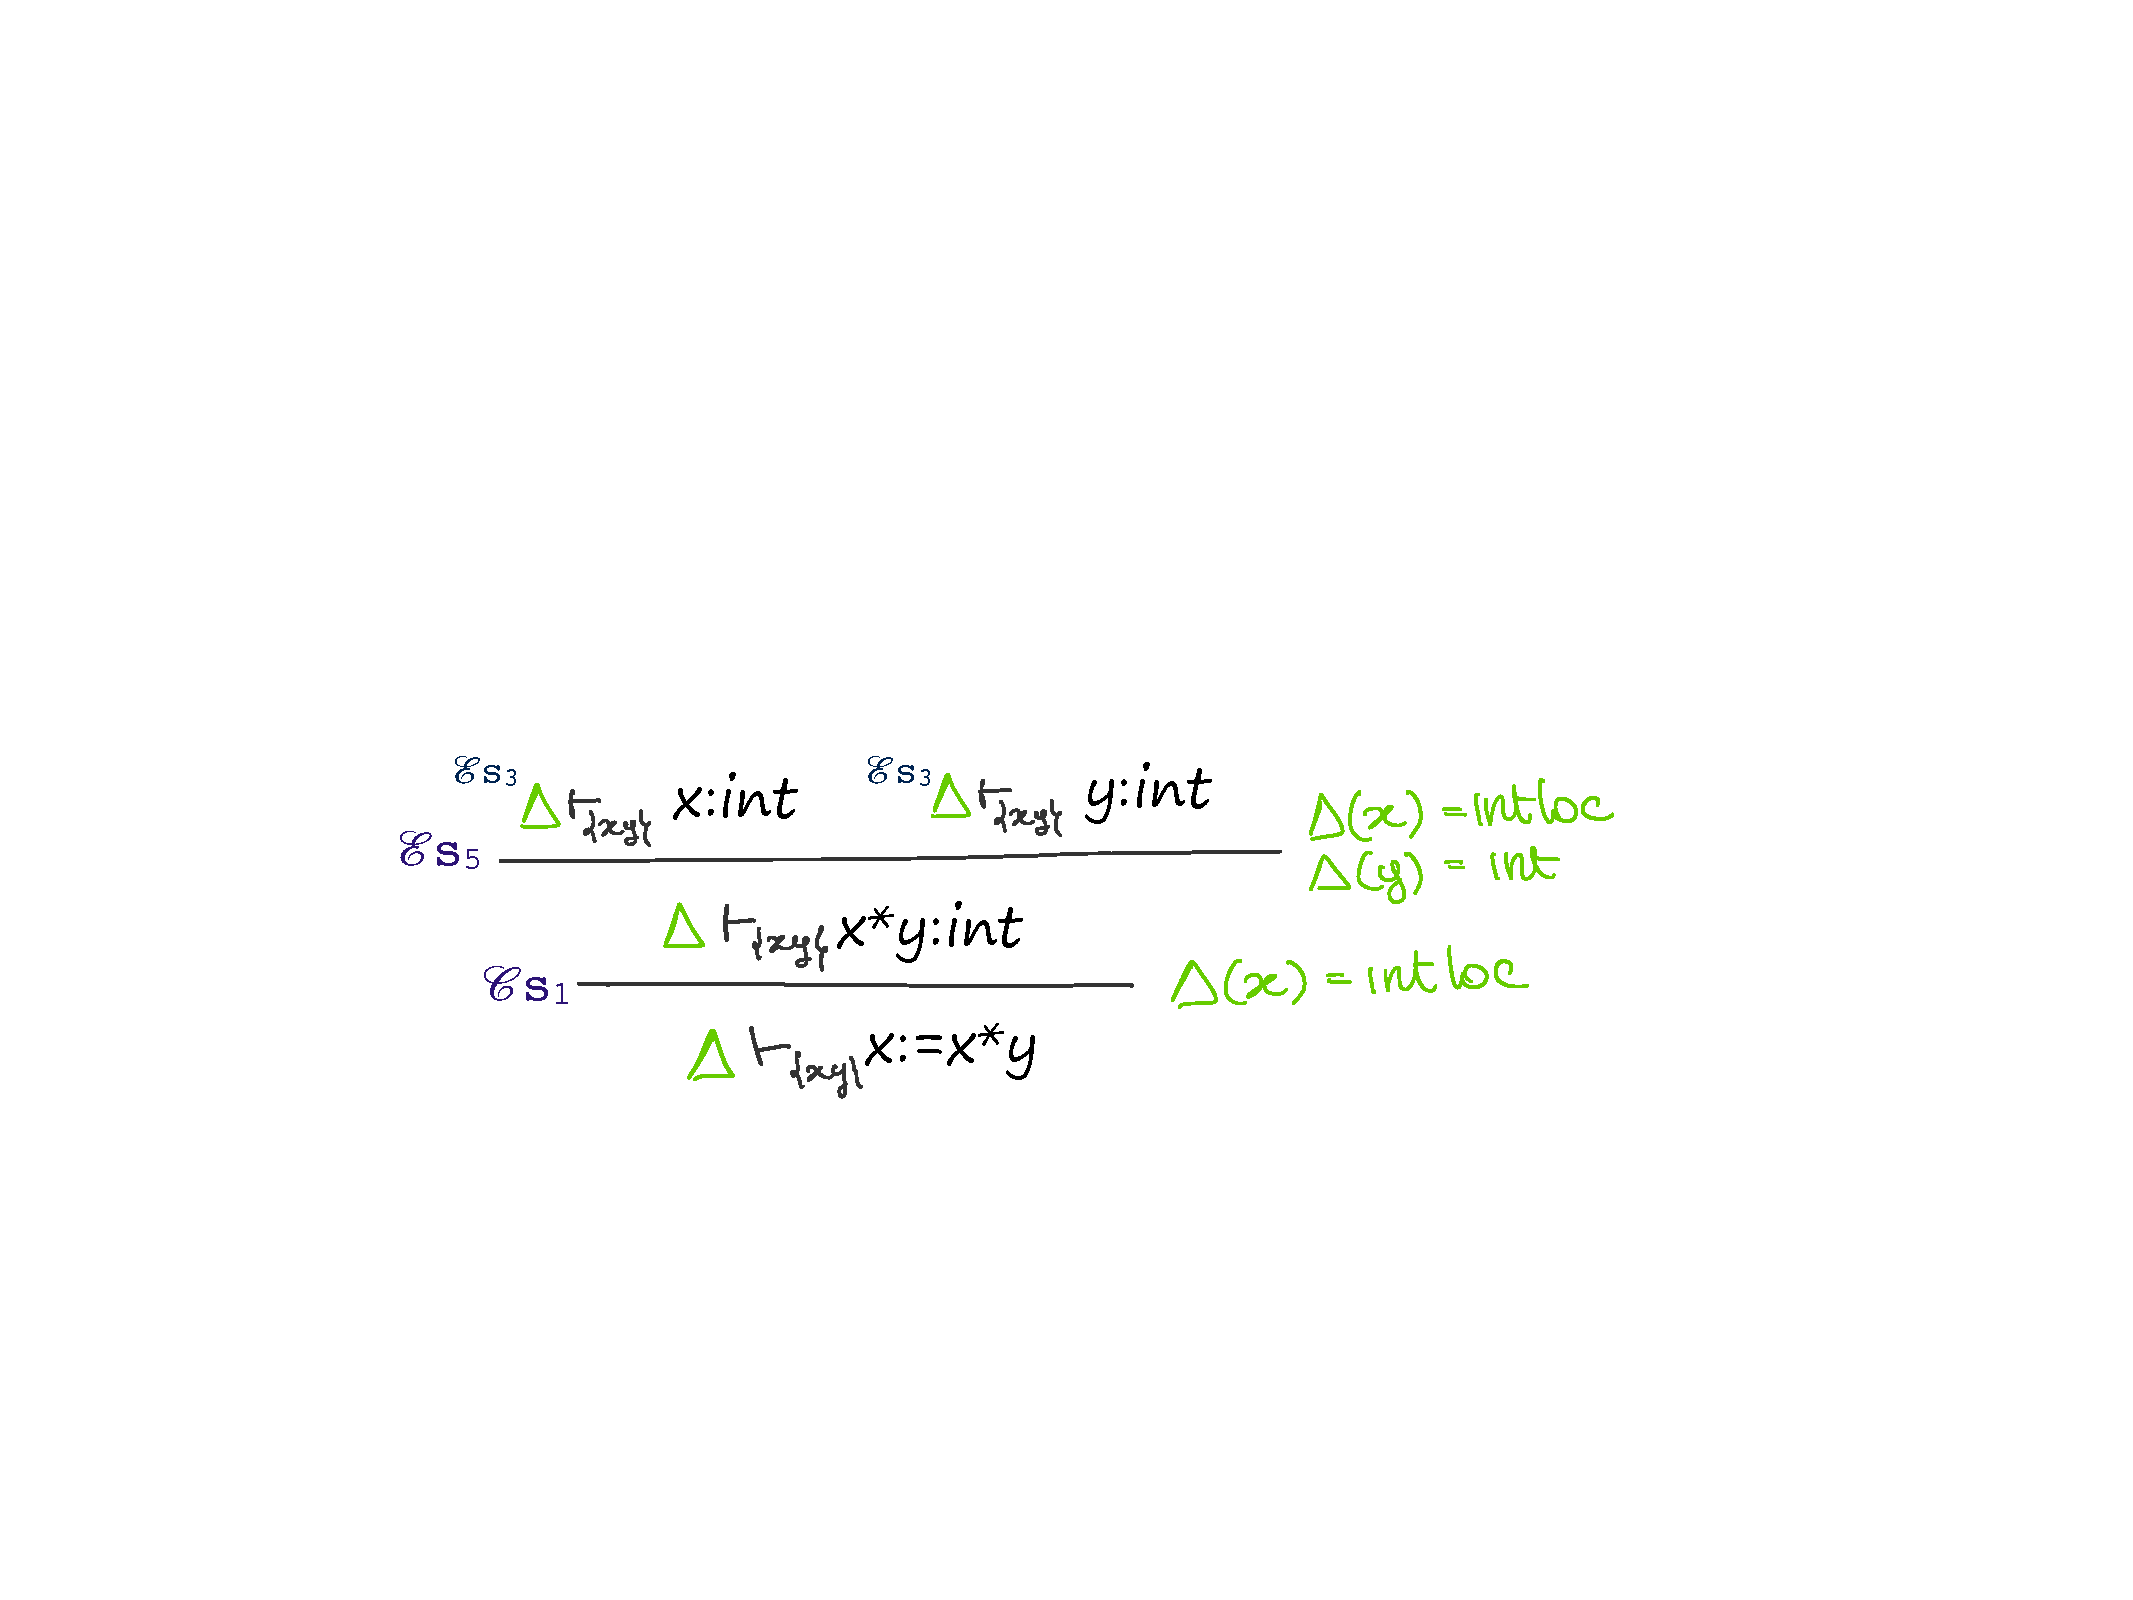
\includegraphics[width=.8\textwidth]{img/esempio_assegnamento_sem-statica.pdf}
 	\end{figure}\newpage
 	
 	\noindent
 	Mentre la dimostrazione per la semantica dinamica:
 	\begin{figure}[!htp]
 		\centering
 		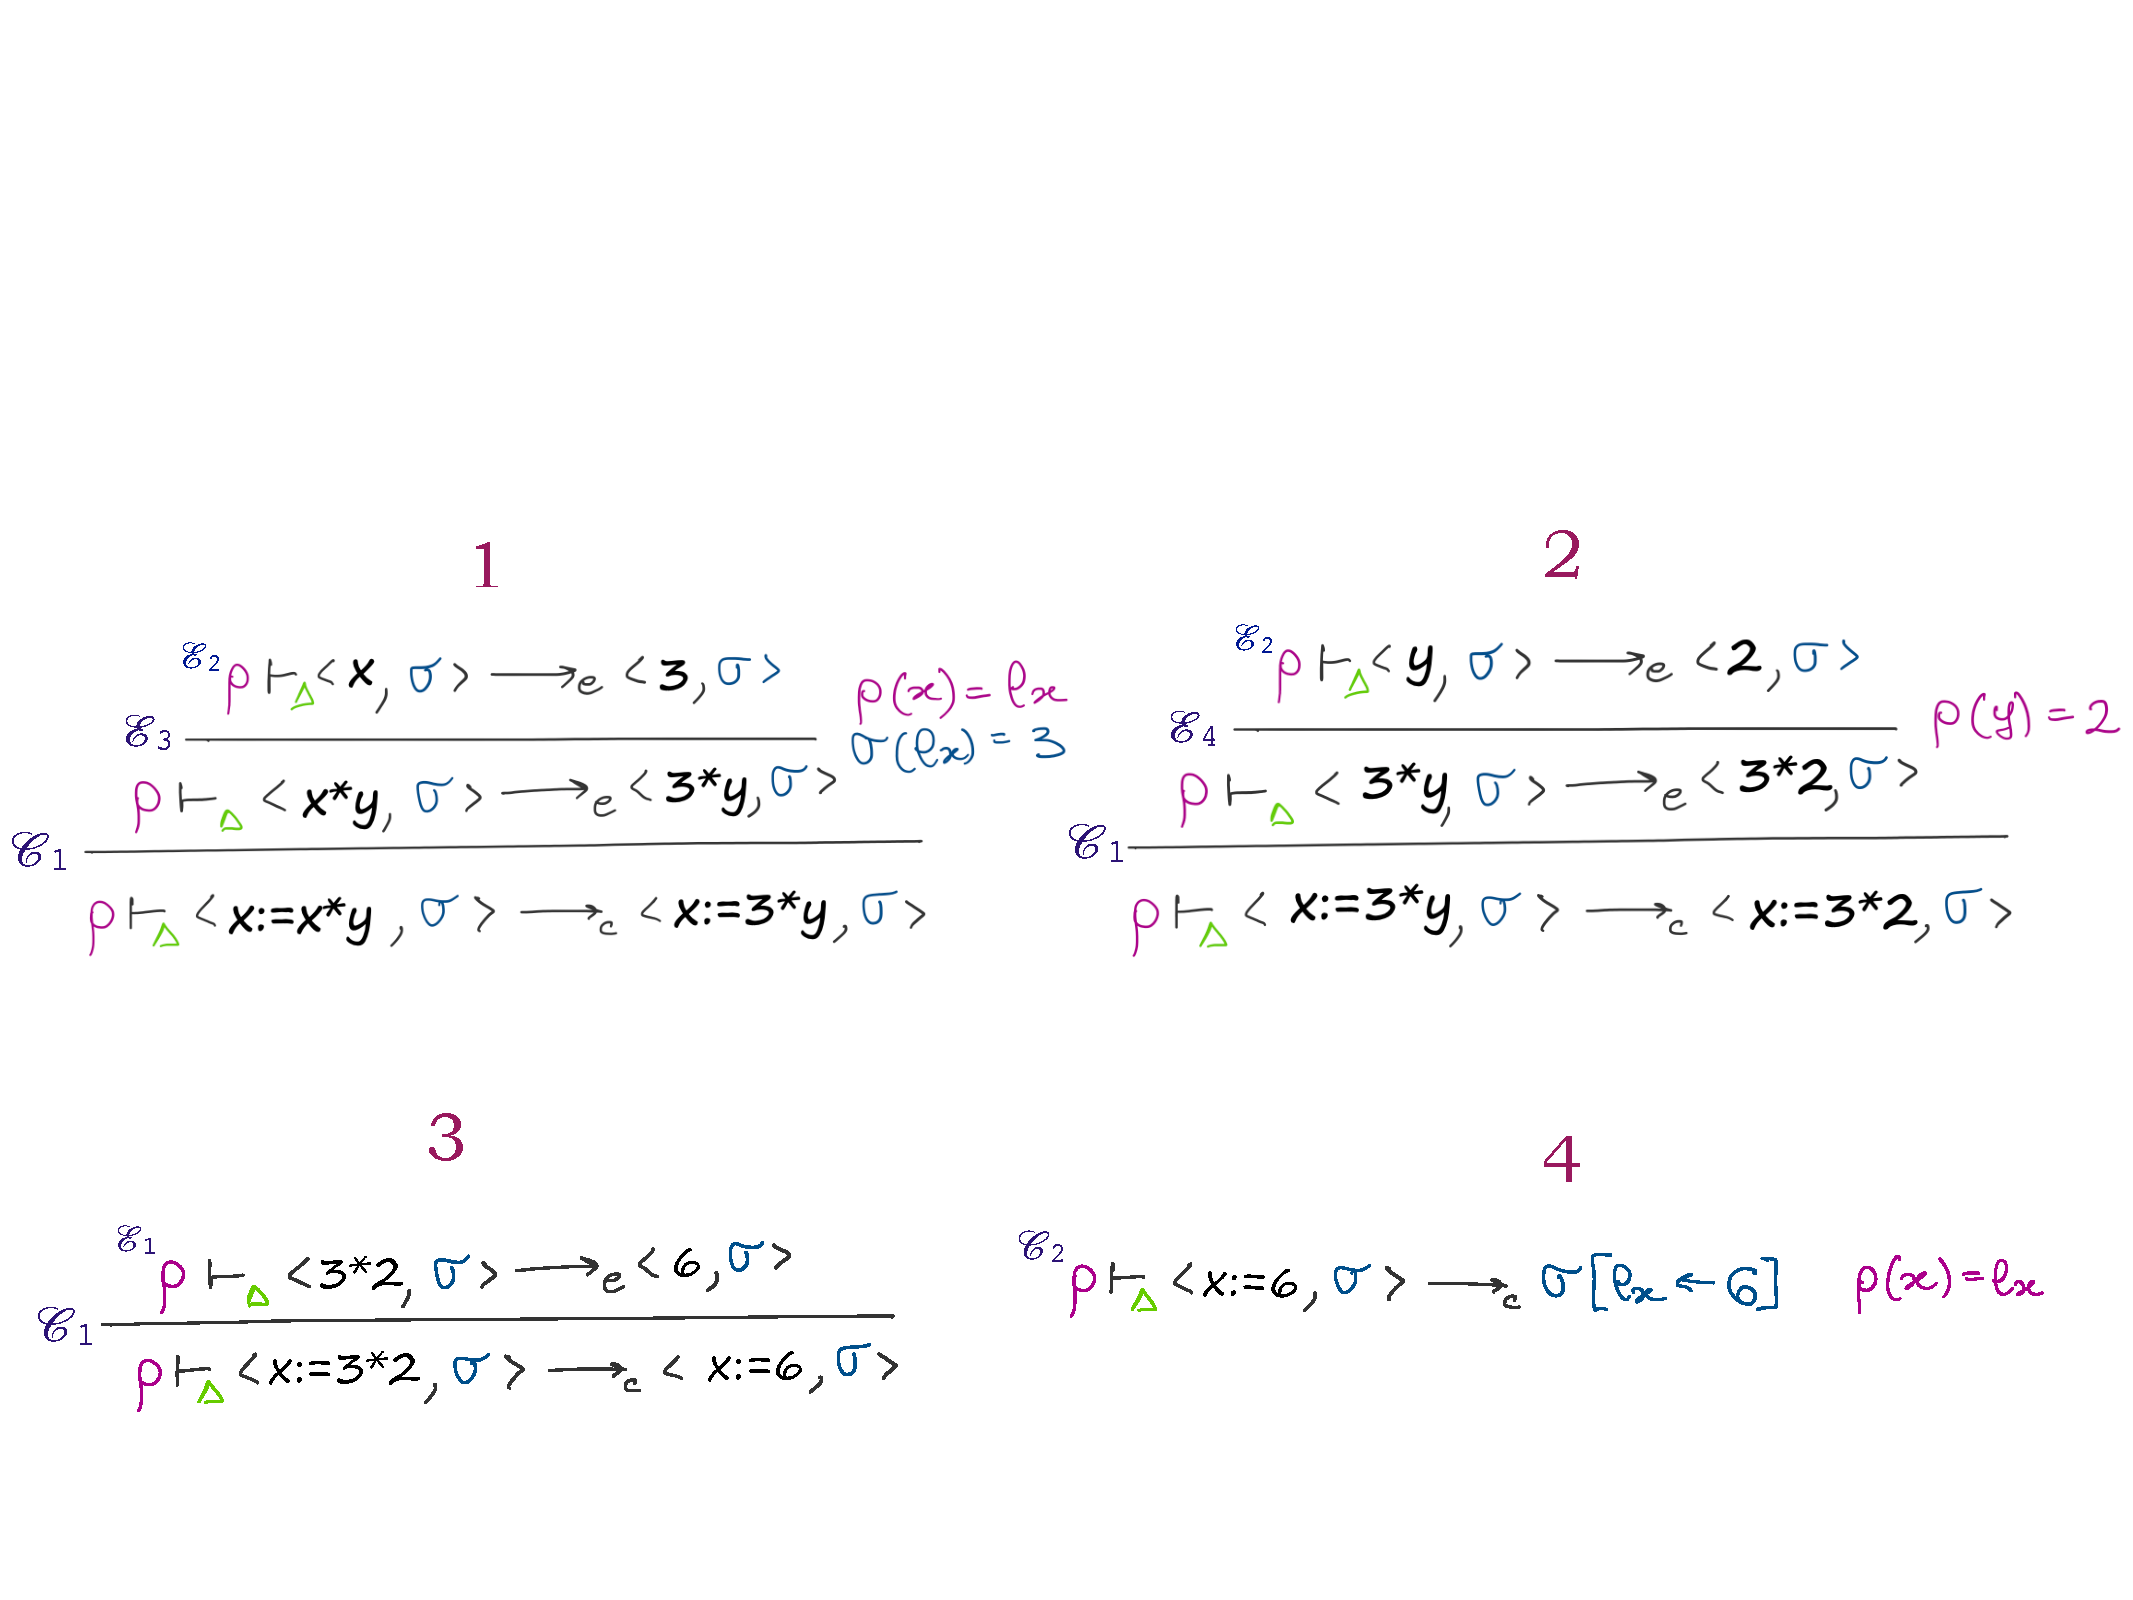
\includegraphics[width=\textwidth]{img/esempio_assegnamento_sem-dinamica.pdf}
 	\end{figure}
 	
 	\longline
 	
 	\subsection{Strutture di controllo}
 	
 	\subsubsection{Selettori}
 	
 	Il \textbf{controllo dell'esecuzione} avviene grazie a delle \textbf{strutture di controllo}, le quali sono comandi che specificano/controllano l'ordine con cui le modifiche (assegnamenti) devono essere fatte. In altre parole, specificano alternative e ripetono comandi. Le strutture di controllo possono trovarsi:
 	\begin{itemize}
 		\item Nelle espressioni;
 		\item Tra comandi;
 		\item Tra unità di programma (procedure).
 	\end{itemize}
 	Una delle \textbf{prime strutture di controllo} sono i \textcolor{Red3}{\textbf{selettori}}, ovvero comandi di selezione. Essi forniscono gli strumenti per scegliere tra due o più cammini di esecuzione: selettori a due vie (comandi condizionali) oppure selettori a più vie. In generale la sua forma è la seguente:
 	\begin{equation*}
 		\begin{array}{ll}
 			\mathsf{if} 	& control\_expression \\
 			\mathsf{then}	& clause \\
 			\mathsf{else}	& clause
 		\end{array}
 	\end{equation*}
 	Durante la progettazione, è necessario considerare alcune caratteristiches:
 	\begin{itemize}
 		\item \textbf{Forma e tipo delle espressioni di controllo}: l'espressione booleana è la più utilizzata. Tuttavia, talvolta è possibile trovare l'aritmetica e in altre occasioni è racchiusa tra parentesi tonde;
 		
 		\item \textbf{Specifica delle clausole \textsf{then} e \textsf{else}}: nei linguaggi moderni, le clausole \textsf{then} e \textsf{else} possono essere sia comandi singoli che composti. Inoltre, possono essere delimitate in vari modi a seconda dei linguaggi;
 		
 		\item \textbf{Specifica dei selettori annidati}: solitamente i linguaggi hanno regole specifiche per risolvere ambiguità in presenza di selettori annidati.
 	\end{itemize}\newpage
 	
 	\subsubsection{Condizionale in $IMP$: \emph{if-then-else}}
 	
 	Il comando condizionale che viene inserito nel linguaggio $IMP$ è il seguente:
 	\begin{equation*}
 		\textsf{if \textcolor{Blue3}{b} then \textcolor{Red3}{C} else \textcolor{Red3}{C}}
 	\end{equation*}
 	Gli identificatori, all'interno del costrutto, si trovano nella seguente posizione:
 	\begin{gather*}
 		FI\left(\mathsf{if} \: e \: \mathsf{then} \: c_{0} \: \mathsf{else} \: c_{1}\right) = FI\left(c_{0}\right) \cup FI\left(c_{1}\right) \cup FI\left(e\right) \\
 		DI\left(\mathsf{if} \: e \: \mathsf{then} \: c_{0} \: \mathsf{else} \: c_{1}\right) = DI\left(c_{0}\right) \cup DI\left(c_{1}\right)
 	\end{gather*}
 	L'insieme degli \textbf{identificatori liberi} sono l'unione di tutti i singoli identificatori liberi presenti nell'espressione e nei due rami condizionali. Mentre gli \textbf{identificatori definiti} sono l'unione di quelli definiti nei comandi (che possono contenere dichiarazioni).\newline
 	
 	\noindent
 	Le \textbf{regole} in questo caso sono le seguenti:
 	\begin{itemize}
 		\item Per la \textbf{semantica statica} è necessario verificare se il comando è ben formato. I vincoli da verificare sono l'espressione di tipo booleano e che i comandi dei rami condizionali siano ben formati:
 		\begin{equation*}
 			\mathcal{E}\mathrm{s}_{2} : \dfrac{
 				\Delta\vdash_{\mathrm{V}} \:\: \mathrm{e:bool} \hspace{1em} \Delta\vdash_{\mathrm{V}} \: \mathrm{c}_{0} \hspace{1em} \Delta\vdash_{\mathrm{V}} \: \mathrm{c}_{1}
 			}{
 				\Delta\vdash_{\mathrm{V}} \:\: \mathbf{if} \:\: \mathrm{e} \:\: \mathbf{then} \:\: \mathrm{c}_{0} \:\: \mathbf{else} \:\: \mathrm{c}_{1}
 			}
 		\end{equation*}
 		
 		\item Per la \textbf{semantica dinamica} è necessario valutare l'espressione di guardia. Se è vera (\emph{true}), allora si prosegue con l'esecuzione di $c_{0}$, altrimenti si prosegue con l'esecuzione di $c_{1}$:
 		\begin{itemize}
 			\item La terza regola:
 			\begin{equation*}
 				\mathcal{E}_{3} : \dfrac{
 					\rho \:\: \vdash_{\Delta} \:\: \left\langle \mathrm{e}, \sigma \right\rangle \rightarrow_{\mathrm{e}} \left\langle \mathrm{e}', \sigma \right\rangle
 				}{
 					\rho \:\: \vdash_{\Delta} \:\: \left\langle \mathbf{if} \:\: \mathrm{e} \:\: \mathbf{then} \:\: \mathrm{c}_{0} \:\: \mathbf{else} \:\: \mathrm{c}_{1}, \sigma \right\rangle \rightarrow_{\mathrm{c}} \left\langle \mathbf{if} \:\: \mathrm{e}' \:\: \mathbf{then} \:\: \mathrm{c}_{0} \:\: \mathbf{else} \:\: \mathrm{c}_{1}, \sigma \right\rangle
 				}
 			\end{equation*}
 			
 			\item La quarta regola:
 			\begin{equation*}
 				\mathcal{E}_{4} : \:\: \rho \:\: \vdash_{\Delta} \:\: \left\langle \mathbf{if} \:\: \mathrm{true} \:\: \mathbf{then} \:\: \mathrm{c}_{0} \:\: \mathbf{else} \:\: \mathrm{c}_{1}, \sigma \right\rangle \rightarrow_{\mathrm{c}} \left\langle \mathrm{c}_{0}, \sigma \right\rangle
 			\end{equation*}
 			
 			\item La quinta regola:
 			\begin{equation*}
 				\mathcal{E}_{5} : \:\: \rho \:\: \vdash_{\Delta} \:\: \left\langle \mathbf{if} \:\: \mathrm{false} \:\: \mathbf{then} \:\: \mathrm{c}_{0} \:\: \mathbf{else} \:\: \mathrm{c}_{1}, \sigma \right\rangle \rightarrow_{\mathrm{c}} \left\langle \mathrm{c}_{1}, \sigma \right\rangle
 			\end{equation*}
 		\end{itemize}
 	\end{itemize}\newpage
 	
 	\noindent
 	Si presenta un \textcolor{Green4}{\textbf{esempio}} della seguente struttura di controllo:
 	\begin{equation*}
 		\textsf{if x=y then x $\coloneq$ 5 else x $\coloneq$ 6}
 	\end{equation*}
 	Supponendo che ci sia il seguente stato iniziale:
 	\begin{equation*}
 		\begin{array}{lll}
 			\rho 		& = & \left[x \leftarrow l_{x}, y \leftarrow 2\right] \\
 			\sigma_{1}	& = & \left[l_{x} \leftarrow 3\right] \\
 			\sigma_{2}	& = & \left[l_{x} \leftarrow 2\right] \\
 			\Delta		& = & \left[x \leftarrow \mathsf{intloc}, y \leftarrow \mathsf{int}\right]
 		\end{array}
 	\end{equation*}
 	
 	\noindent
 	Si dimostra la semantica statica:
 	\begin{figure}[!htp]
 		\centering
 		\includegraphics[width=\textwidth]{img/esempio_assegnamento_imp-1.pdf}
 	\end{figure}
 	
 	\noindent
 	Successivamente la semantica dinamica con $\sigma_{1}$:
 	\begin{figure}[!htp]
 		\centering
 		\includegraphics[width=\textwidth]{img/esempio_assegnamento_imp-2.pdf}
 	\end{figure}\newpage
 	
 	\noindent
 	E $\sigma_{2}$:
 	\begin{figure}[!htp]
 		\centering
 		\includegraphics[width=\textwidth]{img/esempio_assegnamento_imp-3.pdf}
 	\end{figure}
 	
 	\longline
 	
 	\subsection{Composizione e regole transitive}
 	
 	La \textcolor{Red3}{\textbf{composizione sequenziale}}, denotata con il simbolo \dquotes{;}, consente di specificare in modo diretto la composizione di comando denotando il fatto che il comando a destra del simbolo di composizione inizia dopo che il comando a sinistra ha completato l'esecuzione:
 	\begin{equation*}
 		\textsf{C ; C}
 	\end{equation*}
 	La \textbf{semantica della composizione} viene presentata tramite l'introduzione degli identificatori:
 	\begin{gather*}
 		FI\left(c_{0} ; c_{1}\right) = FI\left(c_{0}\right) \cup FI\left(c_{1}\right) \\
 		DI\left(c_{0} ; c_{1}\right) = DI\left(c_{0}\right) \cup DI\left(c_{1}\right)
 	\end{gather*}
 	E delle relative regole riguardanti la semantica statica e dinamica:
 	\begin{itemize}
 		\item Per la \textbf{semantica statica} si ha:
 		\begin{itemize}
 			\item La corretta formattazione (ben formati) dei comandi:
 			\begin{equation*}
 				\mathcal{E}\mathrm{s}_{3} : \dfrac{
 					\Delta\vdash_{\mathrm{V}} \: \mathrm{c}_{0} \hspace{1.5em} \Delta\vdash_{\mathrm{V}} \: \mathrm{c}_{1}
 				}{
 					\Delta\vdash_{\mathrm{V}} \: \mathrm{c}_{0} \: \boldsymbol{;} \: \mathrm{c}_{1}
 				}
 			\end{equation*}
 			
 			\item Il comando nullo, elemento neutro della composizione:
 			\begin{equation*}
 				\mathcal{E}\mathrm{s}_{4} : \Delta\vdash_{\mathrm{V}} \: \mathbf{skip}
 			\end{equation*}
 		\end{itemize}\newpage
 		
 		\item Per la \textbf{semantica dinamica} vi è la composizione che esegue $c_{0}$ e poi a partire dalla memoria risultante, viene eseguito $c_{1}$:
 		\begin{itemize}
 			\item La sesta regola:
 			\begin{equation*}
 				\mathcal{E}_{6} : \:\: \rho \:\: \vdash_{\Delta} \:\: \left\langle \mathbf{skip}, \sigma \right\rangle \rightarrow_{\mathrm{c}} \sigma
 			\end{equation*}
 			
 			\item La settimana regola:
 			\begin{equation*}
 				\mathcal{E}_{7} : \dfrac{
 					\rho \:\: \vdash_{\Delta} \:\: \left\langle \mathrm{c}, \sigma \right\rangle \rightarrow_{\mathrm{c}} \left\langle \mathrm{c}', \sigma' \right\rangle
 				}{
 					\rho \:\: \vdash_{\Delta} \:\: \left\langle \mathrm{c} \: \boldsymbol{;} \: \mathrm{c}_{0}, \sigma \right\rangle \rightarrow_{\mathrm{c}} \left\langle \mathrm{c}' \: \boldsymbol{;} \: \mathrm{c}_{0}, \sigma' \right\rangle
 				}
 			\end{equation*}
 			
 			\item L'ottava regola:
 			\begin{equation*}
 				\mathcal{E}_{8} : \dfrac{
 					\rho \:\: \vdash_{\Delta} \:\: \left\langle \mathrm{c, \sigma} \right\rangle \rightarrow_{\mathrm{c}} \sigma'
 				}{
 					\rho \:\: \vdash_{\Delta} \:\: \left\langle \mathrm{c} \: \boldsymbol{;} \: \mathrm{c}_{0}, \sigma \right\rangle \rightarrow_{\mathrm{c}} \left\langle \mathrm{c}_{0}, \sigma' \right\rangle
 				}
 			\end{equation*}
 		\end{itemize}
 	\end{itemize}
 	Le \textcolor{Red3}{\textbf{regole transitive}} sono le seguenti:
 	\begin{itemize}
 		\item La prima e seconda:
 		\begin{equation*}
 			\mathcal{E}_{1\text{-}2} : \dfrac{
 				\rho \:\: \vdash_{\Delta} \:\: \left\langle \mathrm{e}, \sigma \right\rangle \longrightarrow^{*}_{\mathrm{e}} \left\langle \mathrm{k}, \sigma \right\rangle  
			}{
				\rho \:\: \vdash_{\Delta} \:\: \left\langle \mathrm{x} \coloneq \mathrm{e}, \sigma \right\rangle \longrightarrow_{\mathrm{c}} \sigma\left[\mathrm{l} \leftarrow \mathrm{k}\right]
			} \hspace{1em} \rho\left(\mathrm{x}\right) = 1
 		\end{equation*}
 		
 		\item La terza e quarta:
 		\begin{equation*}
 			\mathcal{E}_{3\text{-}4} : \dfrac{
 				\rho \:\: \vdash_{\Delta} \:\: \left\langle \mathrm{e}, \sigma \right\rangle \longrightarrow^{*}_{\mathrm{e}} \left\langle \mathbf{true}, \sigma \right\rangle
			}
 			{
 				\rho \:\: \vdash_{\Delta} \:\: \left\langle \mathbf{if} \:\: \mathrm{e} \:\: \mathbf{then} \:\: \mathrm{c}_{0} \:\: \mathbf{else} \:\: \mathrm{c}_{1}, \sigma \right\rangle \longrightarrow_{\mathrm{c}} \left\langle \mathrm{c}_{0}, \sigma \right\rangle
			}
 		\end{equation*}
 		
 		\item La terza e quinta:
 		\begin{equation*}
 			\mathcal{E}_{3\text{-}5} : \dfrac{
 				\rho \:\: \vdash_{\Delta} \:\: \left\langle \mathrm{e}, \sigma \right\rangle \longrightarrow^{*}_{\mathrm{e}} \left\langle \mathbf{false}, \sigma \right\rangle
 			}
 			{
 				\rho \:\: \vdash_{\Delta} \:\: \left\langle \mathbf{if} \:\: \mathrm{e} \:\: \mathbf{then} \:\: \mathrm{c}_{0} \:\: \mathbf{else} \:\: \mathrm{c}_{1}, \sigma \right\rangle \longrightarrow_{\mathrm{c}} \left\langle \mathrm{c}_{1}, \sigma \right\rangle
 			}
 		\end{equation*}
 		
 		\item La sesta:
 		\begin{equation*}
 			\mathcal{E}_{6}: \:\: \rho \:\: \vdash_{\Delta} \:\: \left\langle \mathbf{skip}, \sigma \right\rangle \rightarrow_{\mathrm{c}} \sigma
 		\end{equation*}
 		
 		\item La settima e ottava:
 		\begin{equation*}
 			\mathcal{E}_{7\text{-}8} : \dfrac{
 				\rho \:\: \vdash_{\Delta} \:\: \left\langle \mathrm{c}, \sigma \right\rangle \rightarrow_{\mathrm{c}}^{*} \sigma'
 			}{
 				\rho \:\: \vdash_{\Delta} \:\: \left\langle \mathrm{c} \: \boldsymbol{;} \: \mathrm{c}_{0}, \sigma \right\rangle \rightarrow_{\mathrm{c}} \left\langle \mathrm{c}_{0}, \sigma' \right\rangle
 			}
 		\end{equation*}
 	\end{itemize}\newpage
 	
 	\subsection{Altre strutture di controllo}
 	
 	\subsubsection{Comandi iterativi}
 	
 	L'iterazione consente di eseguire uno o più comandi ripetutamente. Esistono due \textbf{tipi di iterazione}:
 	\begin{itemize}
 		\item Iterazione \textcolor{Red3}{\textbf{indeterminata}} quando i cicli sono \textbf{controllati logicamente}, ovvero su un'espressione booleana (\textsf{while}, \textsf{repeat}, ...);
 		
 		\item Iterazione \textcolor{Red3}{\textbf{determinata}} quando i cicli sono \textbf{controllati numericamente}, con numero di ripetizioni determinate al momento dell'inizio del ciclo (\textsf{for}, \textsf{do}, ...).
 	\end{itemize}
 	
 	\longline
 	
 	\subsubsection{Iterazione in $IMP$: \emph{while}}
 	
 	Un comando iterativo nel linguaggio $IMP$ è:
 	\begin{equation*}
 		\textsf{while \textcolor{Blue3}{b} do \textcolor{Red3}{C}}
 	\end{equation*}
 	Gli identificatori di questo costrutto sono:
 	\begin{gather*}
 		FI\left(\mathsf{while} \: e \: \mathsf{do} \: c\right) = FI\left(c\right) \cup FI\left(e\right) \\
 		DI\left(\mathsf{while} \: e \: \mathsf{do} \: c\right) = DI\left(c\right)
 	\end{gather*}
 	Come risulta evidente dagli identificatori, il comando iterativo non altera né l'insieme degli identificatori liberi, che sono l'unione di tutti gli identificatori liberi nell'espressione e nel corpo, né l'insieme degli identificatori definiti, che sono quelli definiti nel corpo.\newline
 	
 	\noindent
 	Le \textbf{regole} nell'iterazione sono:
 	\begin{itemize}
 		\item Per la \textbf{semantica statica} è necessario verificare se il comando è ben formato. I vincoli da verificare sono che l'espressione sia di tipo booleano e che il comando nel corpo sia ben formato:
 		\begin{equation*}
 			\mathcal{E}\mathrm{s}_{5} : \dfrac{
 				\Delta\vdash{\mathrm{V}} \: \mathrm{e:bool} \hspace{1.5em} \Delta\vdash_{\mathrm{V}} \: \mathrm{c}
 			}{
 				\Delta\vdash{\mathrm{V}} \:\: \mathbf{while} \:\: \mathrm{e} \:\: \mathbf{do} \:\: \mathrm{c}
 			}
 		\end{equation*}
 		
 		\item Per la \textbf{semantica dinamica} è necessario valutare l'espressione di guardia e nel caso in cui sia vera (\emph{true}), viene scelto di eseguire $c$, seguito dalla riesecuzione del comando \textsf{while}, altrimenti viene terminata l'esecuzione:
 		\begin{itemize}
 			\item La nona regola:
 			\begin{equation*}
 				\mathcal{E}_{9} : \dfrac{
 					\rho \:\: \vdash_{\Delta} \:\: \left\langle \mathrm{e}, \sigma \right\rangle \rightarrow_{\mathrm{e}}^{*} \left\langle \mathbf{true}, \sigma \right\rangle
 				}{
 					\rho \:\: \vdash_{\Delta} \:\: \left\langle \mathbf{while} \:\: \mathrm{e} \:\: \mathbf{do} \:\: \mathrm{c}, \sigma \right\rangle \rightarrow_{\mathrm{c}} \left\langle \mathrm{c} \: \boldsymbol{;} \: \mathbf{while} \:\: \mathrm{e} \:\: \mathbf{do} \:\: \mathrm{c}, \sigma \right\rangle
 				}
 			\end{equation*}
 			
 			\item La decima regola:
 			\begin{equation*}
 				\mathcal{E}_{10} : \dfrac{
 					\rho \:\: \vdash_{\Delta} \:\: \left\langle \mathrm{e}, \sigma \right\rangle \rightarrow_{\mathrm{e}}^{*} \left\langle \mathbf{false}, \sigma \right\rangle
 				}{
 					\rho \:\: \vdash_{\Delta} \:\: \left\langle \mathbf{while} \:\: \mathrm{e} \:\: \mathbf{do} \:\: \mathrm{c}, \sigma \right\rangle \rightarrow_{\mathrm{c}} \sigma
 				}
 			\end{equation*}
 		\end{itemize}
 	\end{itemize}\newpage
 	
 	\noindent
 	Si riporta qua di seguito un \textcolor{Green4}{\textbf{esempio}} del seguente comando di iterazione:
 	\begin{equation*}
 		\textsf{while not x=0 do x $\coloneq$ x $-$ 1}
 	\end{equation*}
 	Supponendo il seguente stato:
 	\begin{equation*}
 		\begin{array}{lll}
 			\rho 	& = & \left[x \leftarrow l_{x}, y \leftarrow 2\right] \\
 			\sigma	& = & \left[l_{x} \leftarrow 2\right] \\
 			\Delta	& = & \left[x \leftarrow \mathsf{intloc}, y \leftarrow \mathsf{int}\right]
 		\end{array}
 	\end{equation*}
 	Si inizia come sempre dalla dimostrazione della semantica statica:
 	\begin{figure}[!htp]
 		\centering
 		\includegraphics[width=\textwidth]{img/esempio_iterazione_imp-1.pdf}
 	\end{figure}\newpage
 	
 	\noindent
 	Si inizia la dimostrazione della semantica dinamica. Per farlo, si devono eseguire tre iterazioni, poiché con $x\coloneq2$ sono necessarie due iterazioni per ridurre $x$ a zero e un'ultima iterazione per uscire dal ciclo \textsf{while}. Quindi la dimostrazione della prima iterazione:
 	\begin{figure}[!htp]
 		\centering
 		\includegraphics[width=\textwidth]{img/esempio_iterazione_imp-2.pdf}
 	\end{figure}
 	
 	\noindent
 	La seconda iterazione:
 	\begin{figure}[!htp]
 		\centering
 		\includegraphics[width=\textwidth]{img/esempio_iterazione_imp-3.pdf}
 	\end{figure}\newpage
 	
 	\noindent
 	La terza e ultima iterazione:
 	\begin{figure}[!htp]
 		\centering
 		\includegraphics[width=\textwidth]{img/esempio_iterazione_imp-4.pdf}
 	\end{figure}
 	
 	\longline
 	
 	\subsection{Blocchi}\label{blocchi}
 	
 	\subsubsection{Integrazione di ambienti e memorie}
 	
 	Per eseguire un comando che coinvolge le variabili, nasce il bisogno di un costrutto che consenta di identificare l'ambiente in cui un comando viene eseguito. Questo costrutto è chiamato \textcolor{Red3}{\textbf{blocco}}.\newline
 	
 	\noindent
 	Un blocco è una \textbf{regione testuale} che può contenere \textbf{dichiarazioni locali e comandi}. L'\textbf{ambiente} di un blocco è costituito dalle \textbf{associazioni dichiarate localmente}. L'ambiente quindi può cambiare durante l'esecuzione ma tali cambiamenti avvengono generalmente all'entrata e all'uscita di un blocco.\newline
 	
 	\noindent
 	L'\textbf{uso} dei blocchi consente:
 	\begin{itemize}
 		\item Gestione locale dei nomi;
 		\item Aumenta la chiarezza;
 		\item Aumenta la libertà nella scelta dei nomi poiché non ci sono restrizioni;
 		\item Se viene eseguita un'allocazione opportuna, aumenta anche l'ottimizzazione dell'occupazione della memoria.
 	\end{itemize}
 	Inoltre, i blocchi sono identificati da delimitatori, come le parentesi.\newpage
 	
 	\subsubsection{Scope e regole di visibilità}
 	
 	I blocchi non possono essere parzialmente sovrapposti, ovvero o sono disgiunti o sono annidati. Inoltre, possono esistere dei vincoli di annidamento in funzione del linguaggio. Per \textcolor{Green4}{\textbf{esempio}}, in C non si possono dichiarare procedure dentro altre procedure.\newline
 	
 	\noindent
 	Il blocco \textbf{fissa la visibilità delle dichiarazioni ad un insieme di comandi}. Una \textbf{dichiarazione locale ad un blocco è visibile} (\textcolor{Red3}{\textbf{\emph{scope}}}) in quel blocco e in tutti i blocchi in esso annidati. È evidente che è importante stabilire quali sono le \textbf{regole di visibilità}:
 	\begin{boxdef}\label{regola di visibilità}
 		La \textcolor{Red3}{\textbf{regola di visibilità}} è la seguente. Una dichiarazione locale ad un blocco è visibile in quel blocco e in tutti i blocchi in esso annidati, a meno che non intervenga in tali blocchi una nuova dichiarazione dello stesso nome (che nasconde, o maschera, la precedente).
 	\end{boxdef}
 	
	\noindent
	Dalla definizione si deduce che \textbf{ogni definizione annidata genera un buco nello scope precedente}, ovvero nella porzione di codice in cui il \emph{binding} è valido e il nome è utilizzabile con il significato associato.
	
	I \emph{binding} annidati creano \textbf{problemi di leggibilità}, rendono più \textbf{complesso l'individuazione del giusto \emph{binding}} e infine possono \textbf{complicare il \emph{debugging}}. Nonostante questa serie di problemi, il \emph{binding} annidato viene utilizzato date l'opportunità ai programmatori di utilizzare i propri nomi, indipendentemente da altre porzioni di codice.
	
	\begin{boxdef}
		Con \textcolor{Red3}{\textbf{scope (statico)}} ci si riferisce all'area di testo del programma (codice) nel quale tutte le occorrenze applicate di un identificatore si riferiscono alla stessa occorrenza di \emph{binding} dell'identificatore. Così facendo, permette di \textbf{legare} un identificatore al \emph{binding} a tempo di compilazione cercandolo nel blocco che testualmente lo contiene.
	\end{boxdef}\newpage
 	
 	\subsubsection{Tipi di ambienti}
 	
 	Lo \textbf{scope di una variabile (definita)} è il range di comandi ai quali è visibile. Una \textbf{variabile} può essere di \textbf{tre tipi}:
 	\begin{itemize}
 		\item Le \textcolor{Red3}{\textbf{variabili locali}} di un blocco programma sono quelle \textbf{dichiarate nel blocco stesso};
 		
 		\item Le \textcolor{Red3}{\textbf{variabili non locali}} ad un blocco sono quelle visibili al blocco ma non dichiarate in esso. Sono \textbf{dichiarate nel blocco che le contiene};
 		
 		\item Le \textcolor{Red3}{\textbf{variabili globali}} sono come variabili non locali, \textbf{dichiarate nel blocco (globale)} che contiene l'intero programma.
 	\end{itemize}
 	L'esistenza di variabili di tipo diverso rispetto alla regione in cui sono definite determina la caratterizzazione di \textbf{diversi tipi} di \textbf{ambienti}:
 	\begin{itemize}
 		\item \textcolor{Red3}{\textbf{Ambiente locale}}: le \textbf{associazioni vengono create all'ingresso} del blocco (variabili locali e parametri formali);
 		
 		\item \textcolor{Red3}{\textbf{Ambiente non locale}}: le \textbf{associazioni vengono ereditate da altri blocchi} e sono dunque visibili al blocco stesso;
 		
 		\item \textcolor{Red3}{\textbf{Ambiente globale}}: sono le \textbf{associazioni comuni a tutti i blocchi}, ovvero dichiarazioni esplicite di variabili globali, dichiarazioni del blocco più esterno e associazioni esportate da modulo, ecc.
 	\end{itemize}\newpage
 	
 	\subsubsection{Tempo di vita}
 	
 	Le variabili hanno un \textcolor{Red3}{\textbf{tempo di vita}}. Esso consiste nel \textbf{tempo di esecuzione} nel quale tutte le \textbf{occorrenze applicate}, di un identificatore, si \textbf{riferiscono alla stessa locazione di memoria} legata all'identificatore. Quindi, il \textbf{tempo di vita di una variabile inizia quando viene legata ad una specifica cella (allocazione) e termina quando il legame viene sciolto (deallocazione)}.\newline
 	
 	\noindent
 	Esiste una \textbf{differenza} tra \textbf{scope (statico)} e \textbf{tempo di vita (\emph{lifetime})}:
 	\begin{itemize}
 		\item Lo \textbf{scope} (statico) è un \textbf{concetto spaziale} e viene \textbf{definito a tempo di compilazione};
 		
 		\item Il \textbf{tempo di vita} (\emph{lifetime}) è un \textbf{concetto temporale} e viene \textbf{definito a tempo di esecuzione}.
 	\end{itemize}
 	Il \textbf{tempo di vita dipende dal tipo di allocazione} degli identificatori che può essere statico o dinamico. In particolare, durante l'esecuzione, il tempo di vita rappresenta quando un identificatore è utilizzabile. Inoltre, il \textbf{tempo di vita inizia all'entrata di un blocco} e \textbf{termina}:
 	\begin{itemize}
 		\item All'\textbf{uscita del blocco} se vi è \textbf{allocazione dinamica};
 		\item Alla \textbf{fine dell'esecuzione del programma} se vi è \textbf{allocazione statica}.
 	\end{itemize}
 	Un \textcolor{Green4}{\textbf{esempio}}:
 	\begin{figure}[!htp]
 		\centering
 		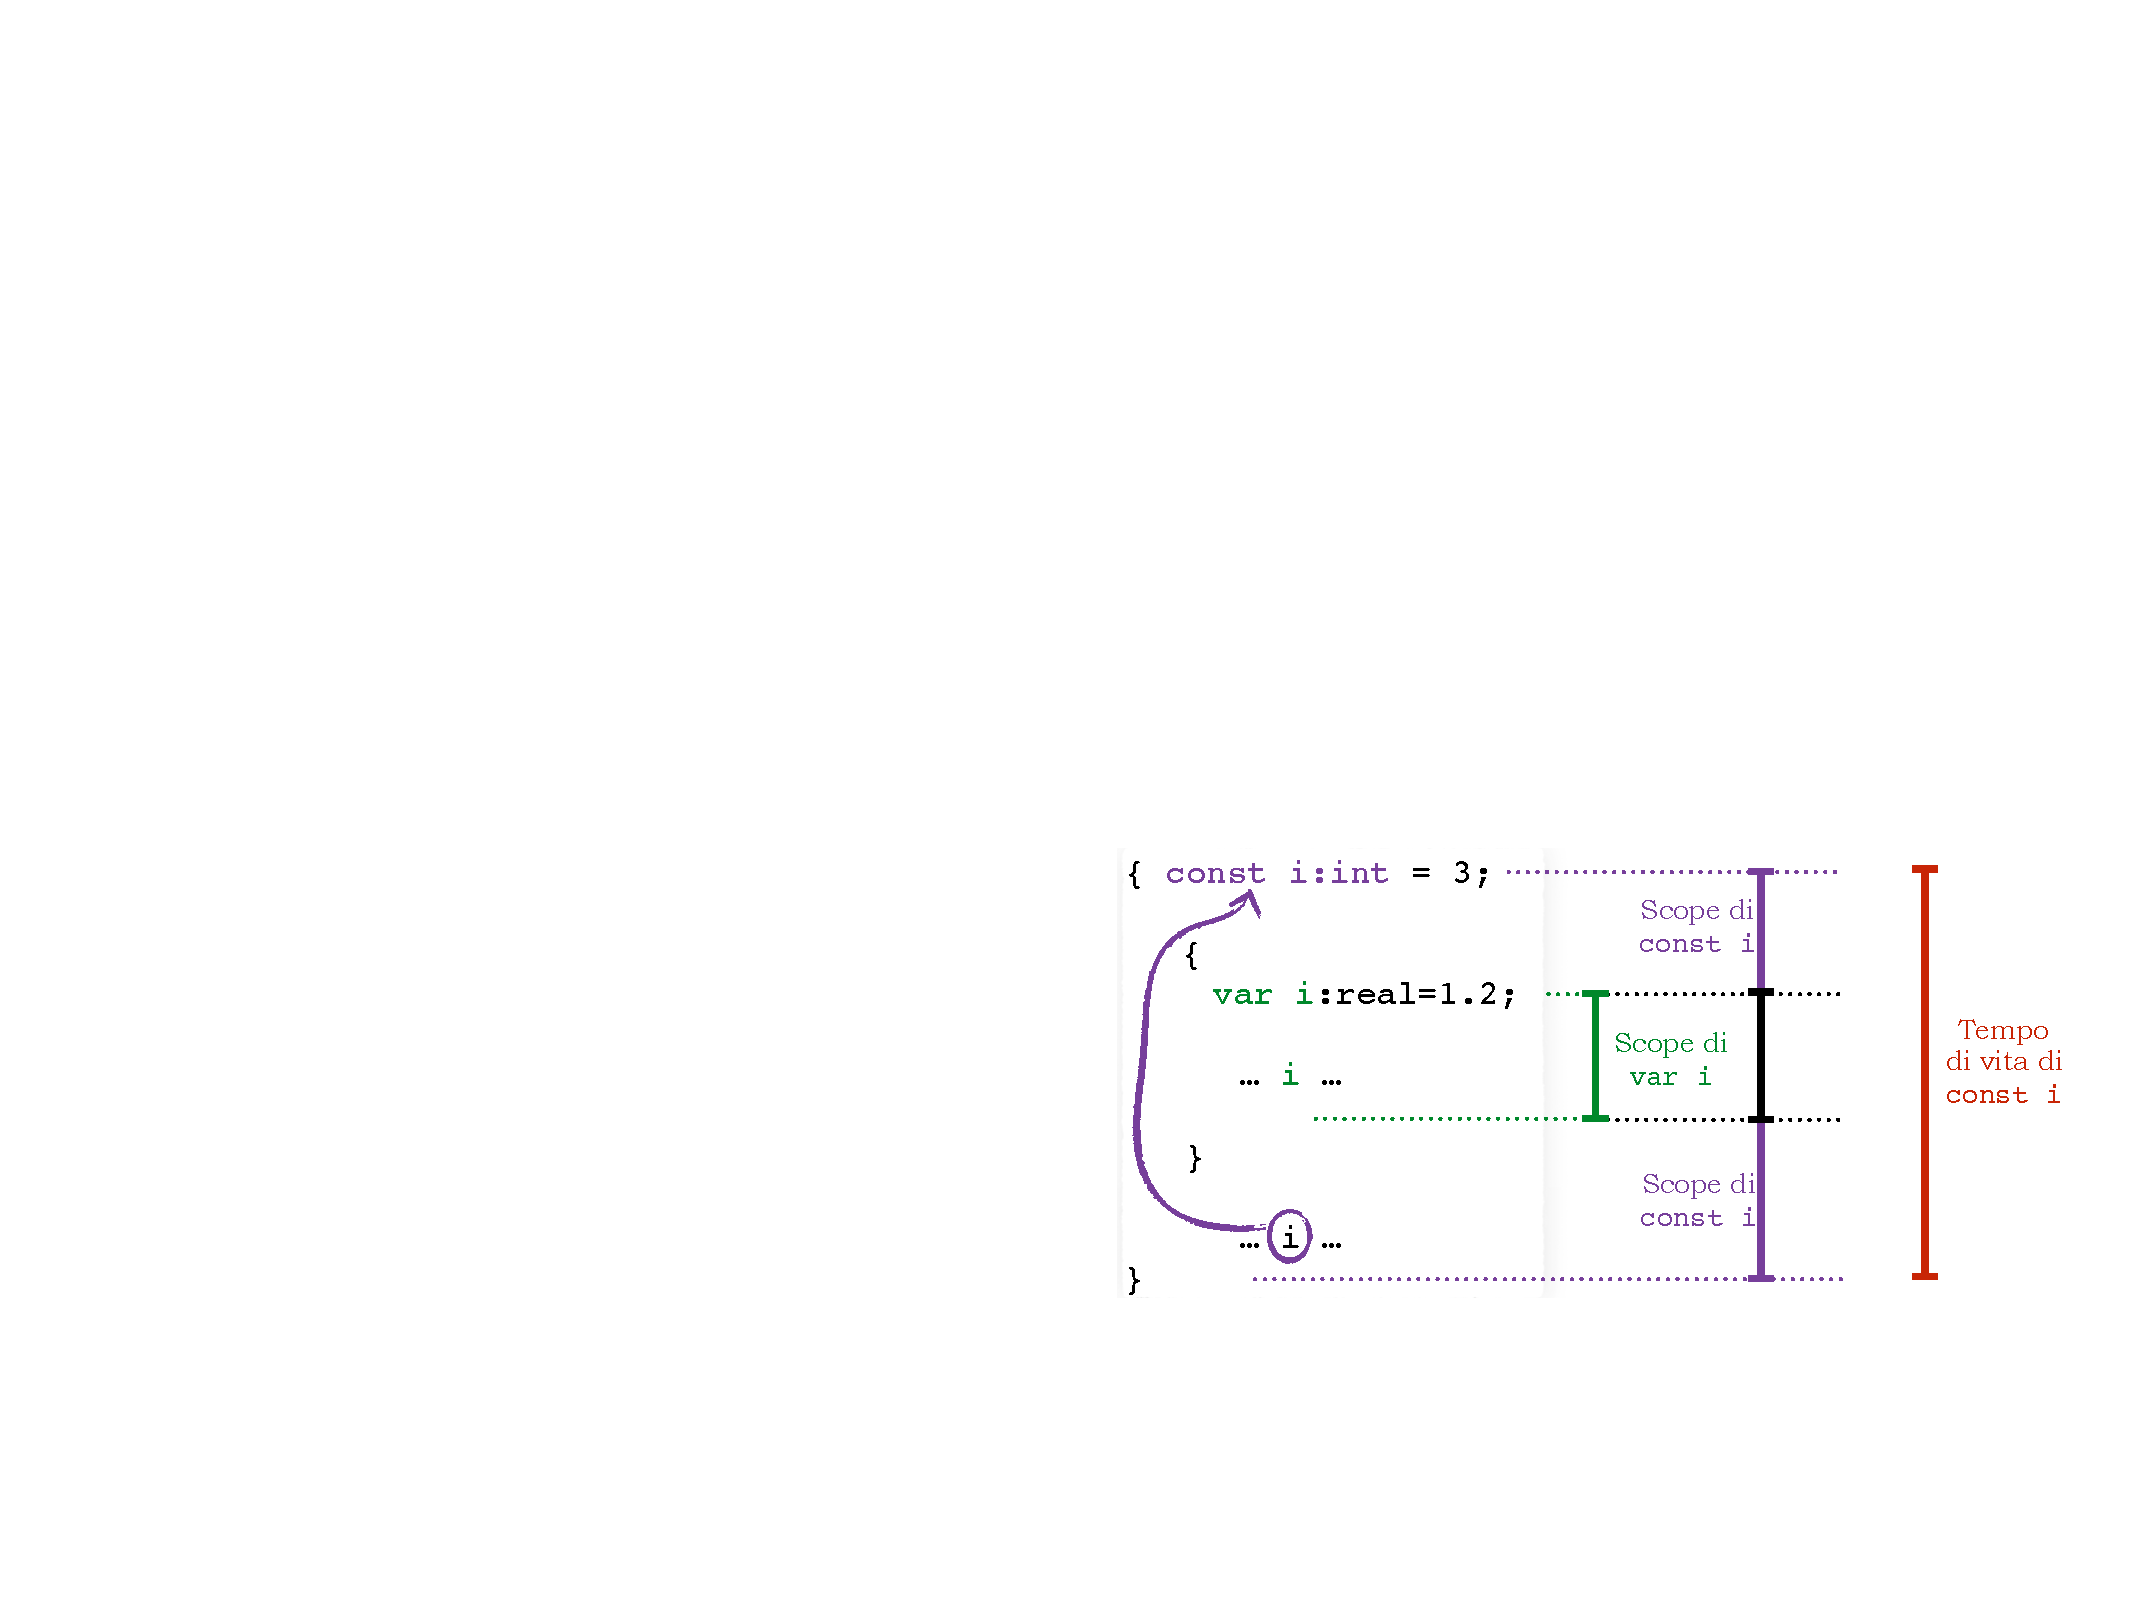
\includegraphics[width=\textwidth]{img/esempio-tempo_di_vita.pdf}
 	\end{figure}\newpage
 	
 	\noindent
 	Un altro \textcolor{Green4}{\textbf{esempio}} più completo è il seguente. Dato il programma:
 	\lstinputlisting[language=C]{code/esempio-tempo_di_vita.txt}
 	Il grafico della memoria:
 	\begin{figure}[!htp]
 		\centering
 		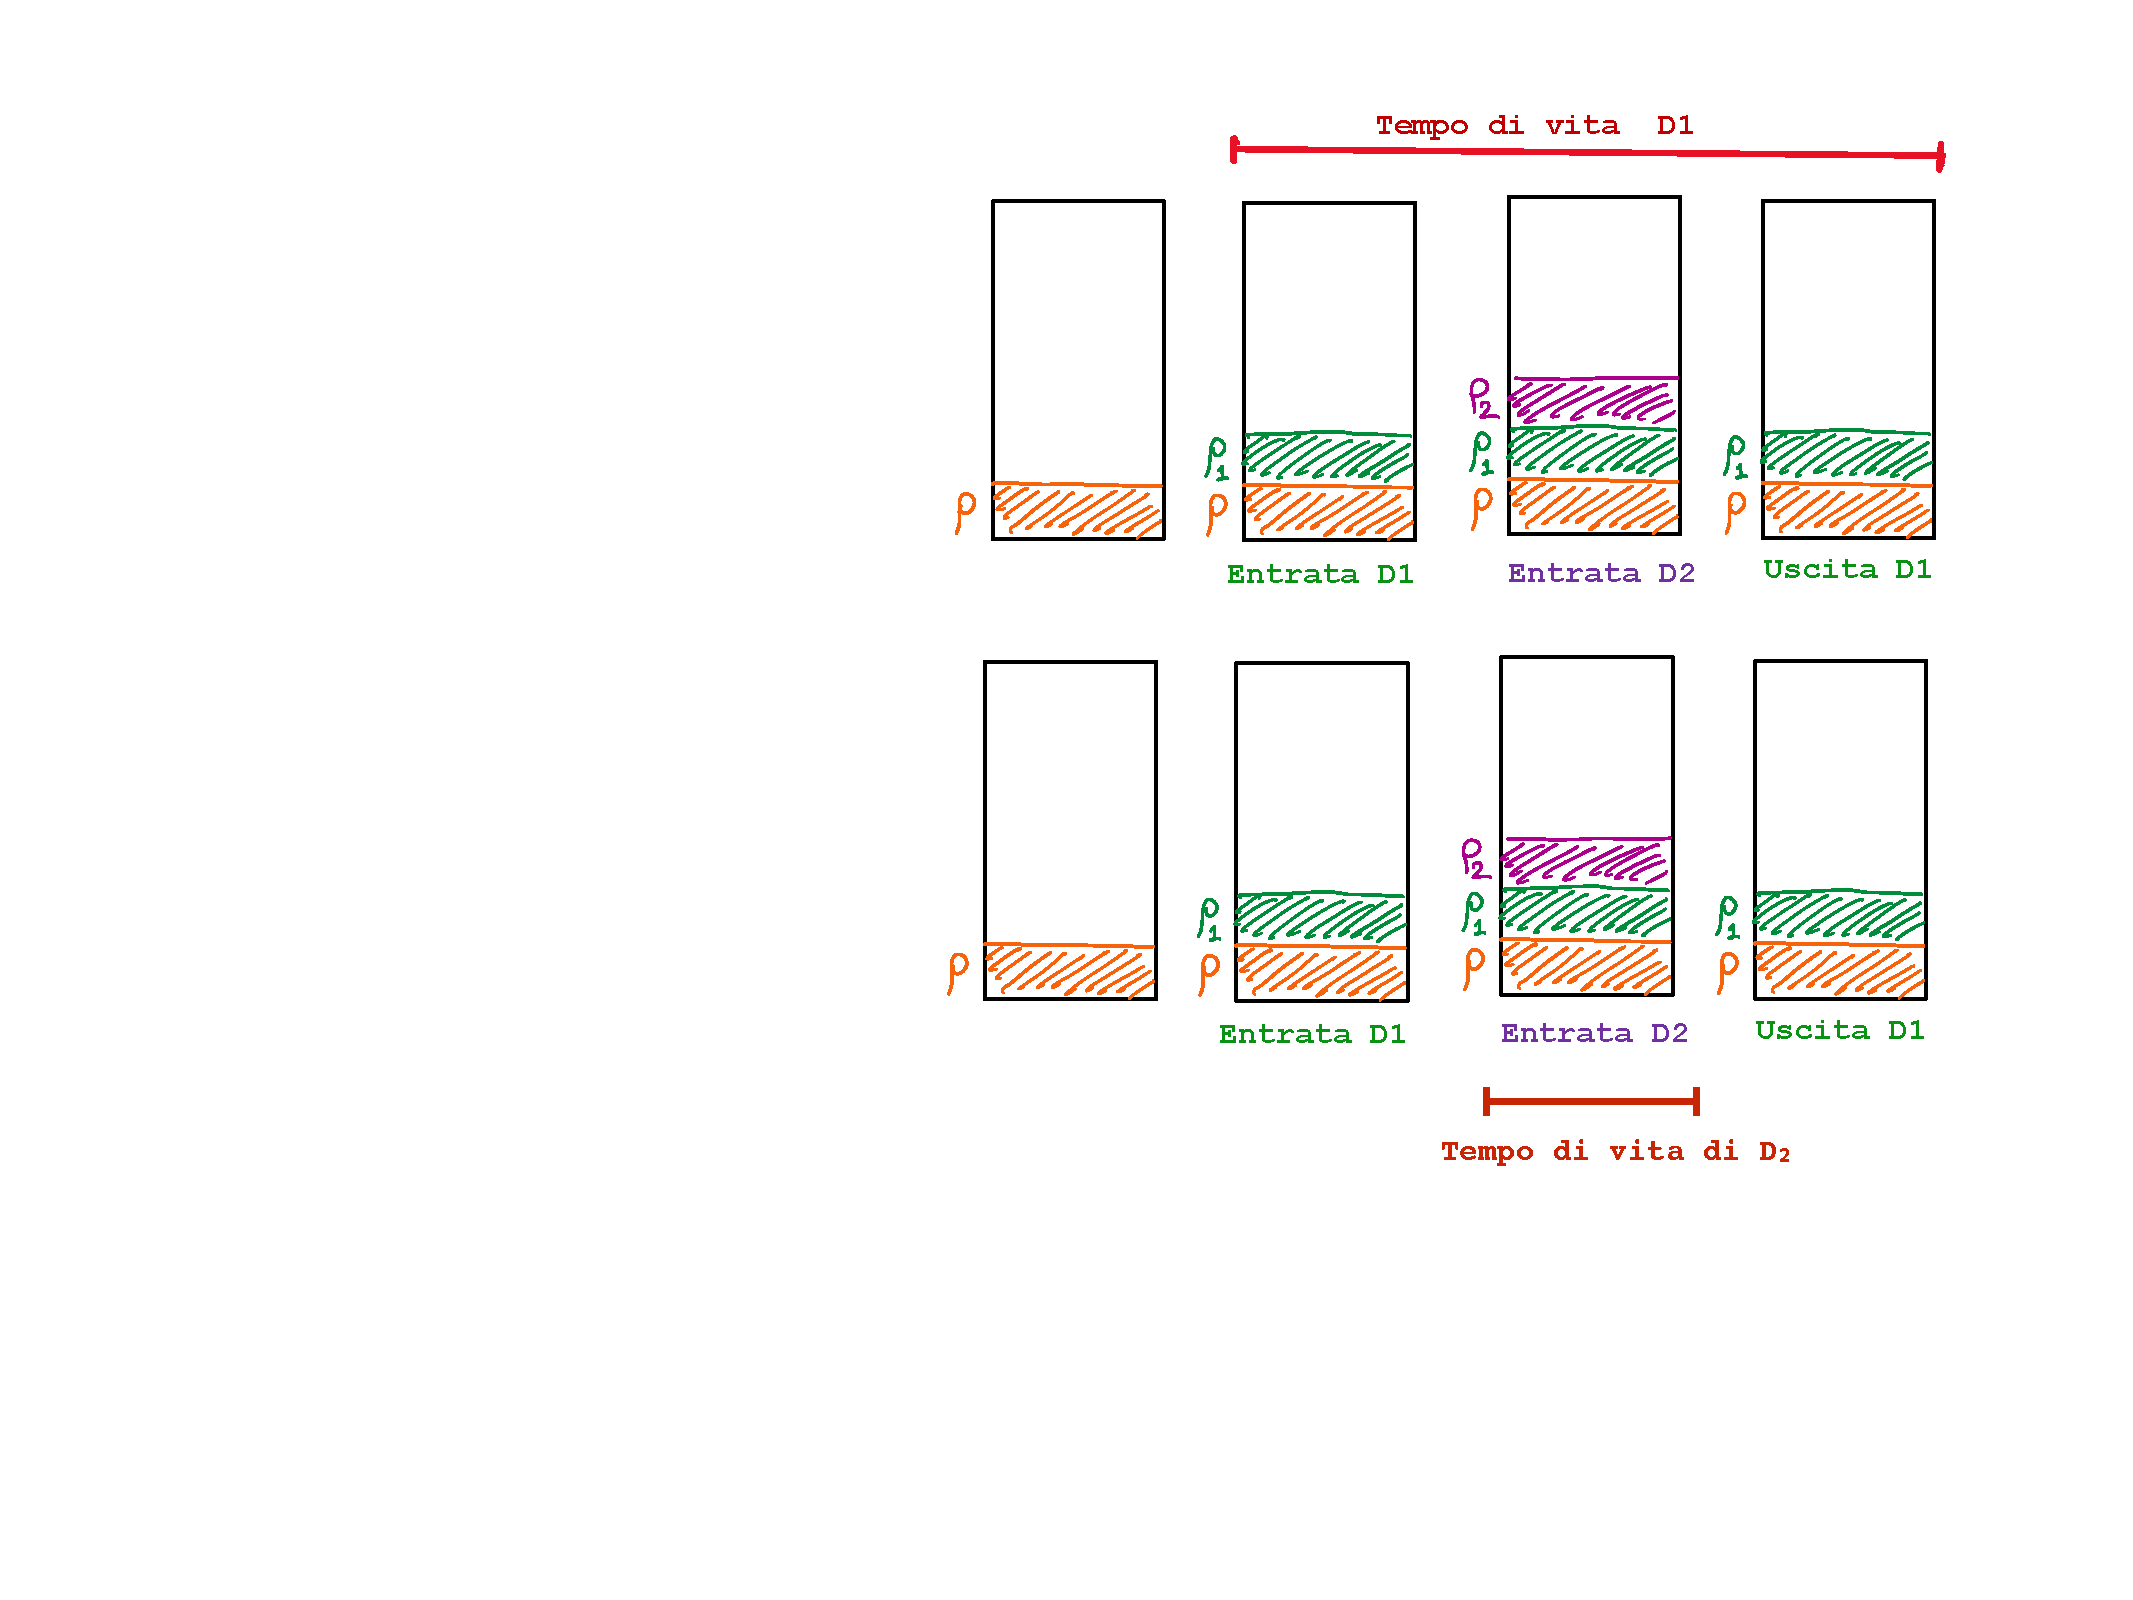
\includegraphics[width=\textwidth]{img/esempio-tempo_di_vita-2.pdf}
 	\end{figure}
 	
 	\noindent
 	Le modifiche generate dalle dichiarazioni sono reversibili. All'uscita di un blocco automaticamente tutte le modifiche fatte dalle dichiarazioni vengono annullate tornando esattamente all'ambiente valido prima di entrare nel blocco. I tempi di vita sono diversi perché, anche se i nomi sono gli stessi e legati allo stesso scope, comunque saranno legati a locazioni diversi a causa della deallocazione. Quest'ultima provoca una perdita delle locazioni precedenti e continuando ad allocare, si creano ipoteticamente nuove allocazioni.
 	
 	\longline
 	
 	\subsubsection{Blocchi in $IMP$}
 	
 	Nel linguaggio $IMP$ è stato inserito il blocco:
 	\begin{equation*}
 		\textsf{D ; C}
 	\end{equation*}
 	Il quale, ha gli identificatori in posizione:
 	\begin{equation*}
 		\begin{array}{lll}
 			FI\left(d;c\right) = FI\left(d\right) \cup \left(\frac{FI\left(c\right)}{DI\left(d\right)}\right)\\
 			DI\left(d;c\right) = DI\left(c\right) \cup DI\left(d\right)
 		\end{array}
 	\end{equation*}
 	Quindi, nel blocco, tutti gli identificatori liberi della dichiarazione sono liberi, mentre sono liberi gli identificatori del comando che non vengono definiti nella dichiarazione. Invece, per gli identificatori definiti, viene presa l'unione di quelli definiti nella dichiarazione e nel comando.\newline
 	
 	\noindent
 	Le \textbf{regole} in questo caso sono:
 	\begin{itemize}
 		\item Per la \textbf{semantica statica} è necessario generare l'ambiente statico $\Delta'$ associato alla dichiarazione $d$ e, nell'ambiente statico $\Delta$ del contesto aggiornato, da $\Delta'$, viene verificato che il comando sia ben formato:
 		\begin{equation*}
 			\mathcal{E}\mathrm{s}_{6} : \dfrac{
 				\Delta\vdash_{\mathrm{V}} \: \mathrm{d}:\Delta' \hspace{1.5em} \Delta\left[\Delta'\right] \: \vdash_{\mathrm{V} \cup \mathrm{V}'} \: \mathrm{c}
 			}{
 				\Delta\vdash_{\mathrm{V}} \: \mathrm{d} \: \boldsymbol{;} \: \mathrm{c}
 			} \:\: \Delta' \:\: \text{su} \:\: \mathrm{V}'
 		\end{equation*}
 		
 		\item Per la \textbf{semantica dinamica}, è necessario elaborare la dichiarazione, la quale può causare \emph{side effects} nella memoria a causa della potenziale definizione di variabili. Successivamente, viene eseguito il comando nell'ambiente modificato della dichiarazione:
 		\begin{itemize}
 			\item Regola undici:
 			\begin{equation*}
 				\mathcal{E}_{11}: \dfrac{
 					\rho \:\: \vdash_{\Delta} \:\: \left\langle \mathrm{d}, \sigma \right\rangle \rightarrow_{\mathrm{d}} \left\langle \mathrm{d}', \sigma' \right\rangle
 				}{
 					\rho \:\: \vdash_{\Delta} \:\: \left\langle \mathrm{d} \: \mathbf{;} \: \mathrm{c}, \sigma \right\rangle \rightarrow_{\mathrm{c}} \left\langle \mathrm{d}' \: \boldsymbol{;} \: \mathrm{c}, \sigma' \right\rangle
 				}
 			\end{equation*}
 			
 			\item In questa regola si vede il concetto di reversibilità. L'ambiente $\rho'$ è temporaneo, così come tutte le modifiche che esegue (anche alla memoria):
 			\begin{equation*}
 				\mathcal{E}_{12} : \dfrac{
 					\rho\left[\rho'\right] \:\: \vdash_{\Delta\left[\Delta'\right]} \:\: \left\langle \mathrm{c}, \sigma \right\rangle \rightarrow_{\mathrm{c}} \left\langle \mathrm{c}', \sigma' \right\rangle
 				}{
 					\rho \:\: \vdash_{\Delta} \:\: \left\langle \rho' \: \mathbf{;} \: \mathrm{c}, \sigma \right\rangle \rightarrow_{\mathrm{c}} \left\langle \rho' \: \boldsymbol{;} \: \mathrm{c}', \sigma' \right\rangle
 				} \:\: \rho' \:\: \vdash_{\Delta'}
 			\end{equation*}
 			
 			\item Regola tredici:
 			\begin{equation*}
 				\mathcal{E}_{13} : \dfrac{
 					\rho\left[\rho'\right] \:\: \vdash_{\Delta\left[\Delta'\right]} \:\: \left\langle \mathrm{c}, \sigma \right\rangle \rightarrow_{\mathrm{c}} \sigma'
 				}{
 					\rho \:\: \vdash_{\Delta} \:\: \left\langle \rho' \: \mathbf{;} \: \mathrm{c}, \sigma \right\rangle \rightarrow_{\mathrm{c}} \sigma'
 				} \:\: \rho' \:\: \vdash_{\Delta'}
 			\end{equation*}
 		\end{itemize}
 	\end{itemize}\newpage
 	
 	\noindent
 	Infine, le regole transitive:
 	\begin{itemize}
 		\item La regola undici e dodici:
 		\begin{equation*}
 			\mathcal{E}_{11\text{-}12} : \dfrac{
 				\rho \:\: \vdash_{\Delta} \:\: \left\langle \mathrm{d}, \sigma \right\rangle \rightarrow^{*}_{\mathrm{d}} \left\langle \rho', \sigma' \right\rangle
 			}{
 				\rho \:\: \vdash_{\Delta} \:\: \left\langle \mathrm{d} \: \boldsymbol{;} \: \mathrm{c}, \sigma \right\rangle \rightarrow_{\mathrm{c}} \left\langle \rho' \: \boldsymbol{;} \: \mathrm{c}, \sigma' \right\rangle
 			}
 		\end{equation*}
 		
 		\item La regola tredici e dodici:
 		\begin{equation*}
 			\mathcal{E}_{13\text{-}12} : \dfrac{
 				\rho\left[\rho'\right] \:\: \vdash_{\Delta\left[\Delta'\right]} \:\: \left\langle \mathrm{c}, \sigma \right\rangle \rightarrow_{\mathrm{c}}^{*} \sigma'
 			}{
 				\rho \:\: \vdash_{\Delta} \:\: \left\langle \rho' \: \boldsymbol{;} \: \mathrm{c}, \sigma \right\rangle \rightarrow_{\mathrm{c}} \sigma'
 			} \:\: \rho' \:\: \vdash_{\Delta'}
 		\end{equation*}
 	\end{itemize}\:\newline
 	
 	\noindent
 	Un \textcolor{Green4}{\textbf{esempio}} è data dalla seguente espressione:
 	\begin{equation*}
 		\textsf{var x:int=3; x $\coloneq$ x+1}
 	\end{equation*}
 	La dimostrazione di semantica statica:
 	\begin{figure}[!htp]
 		\centering
 		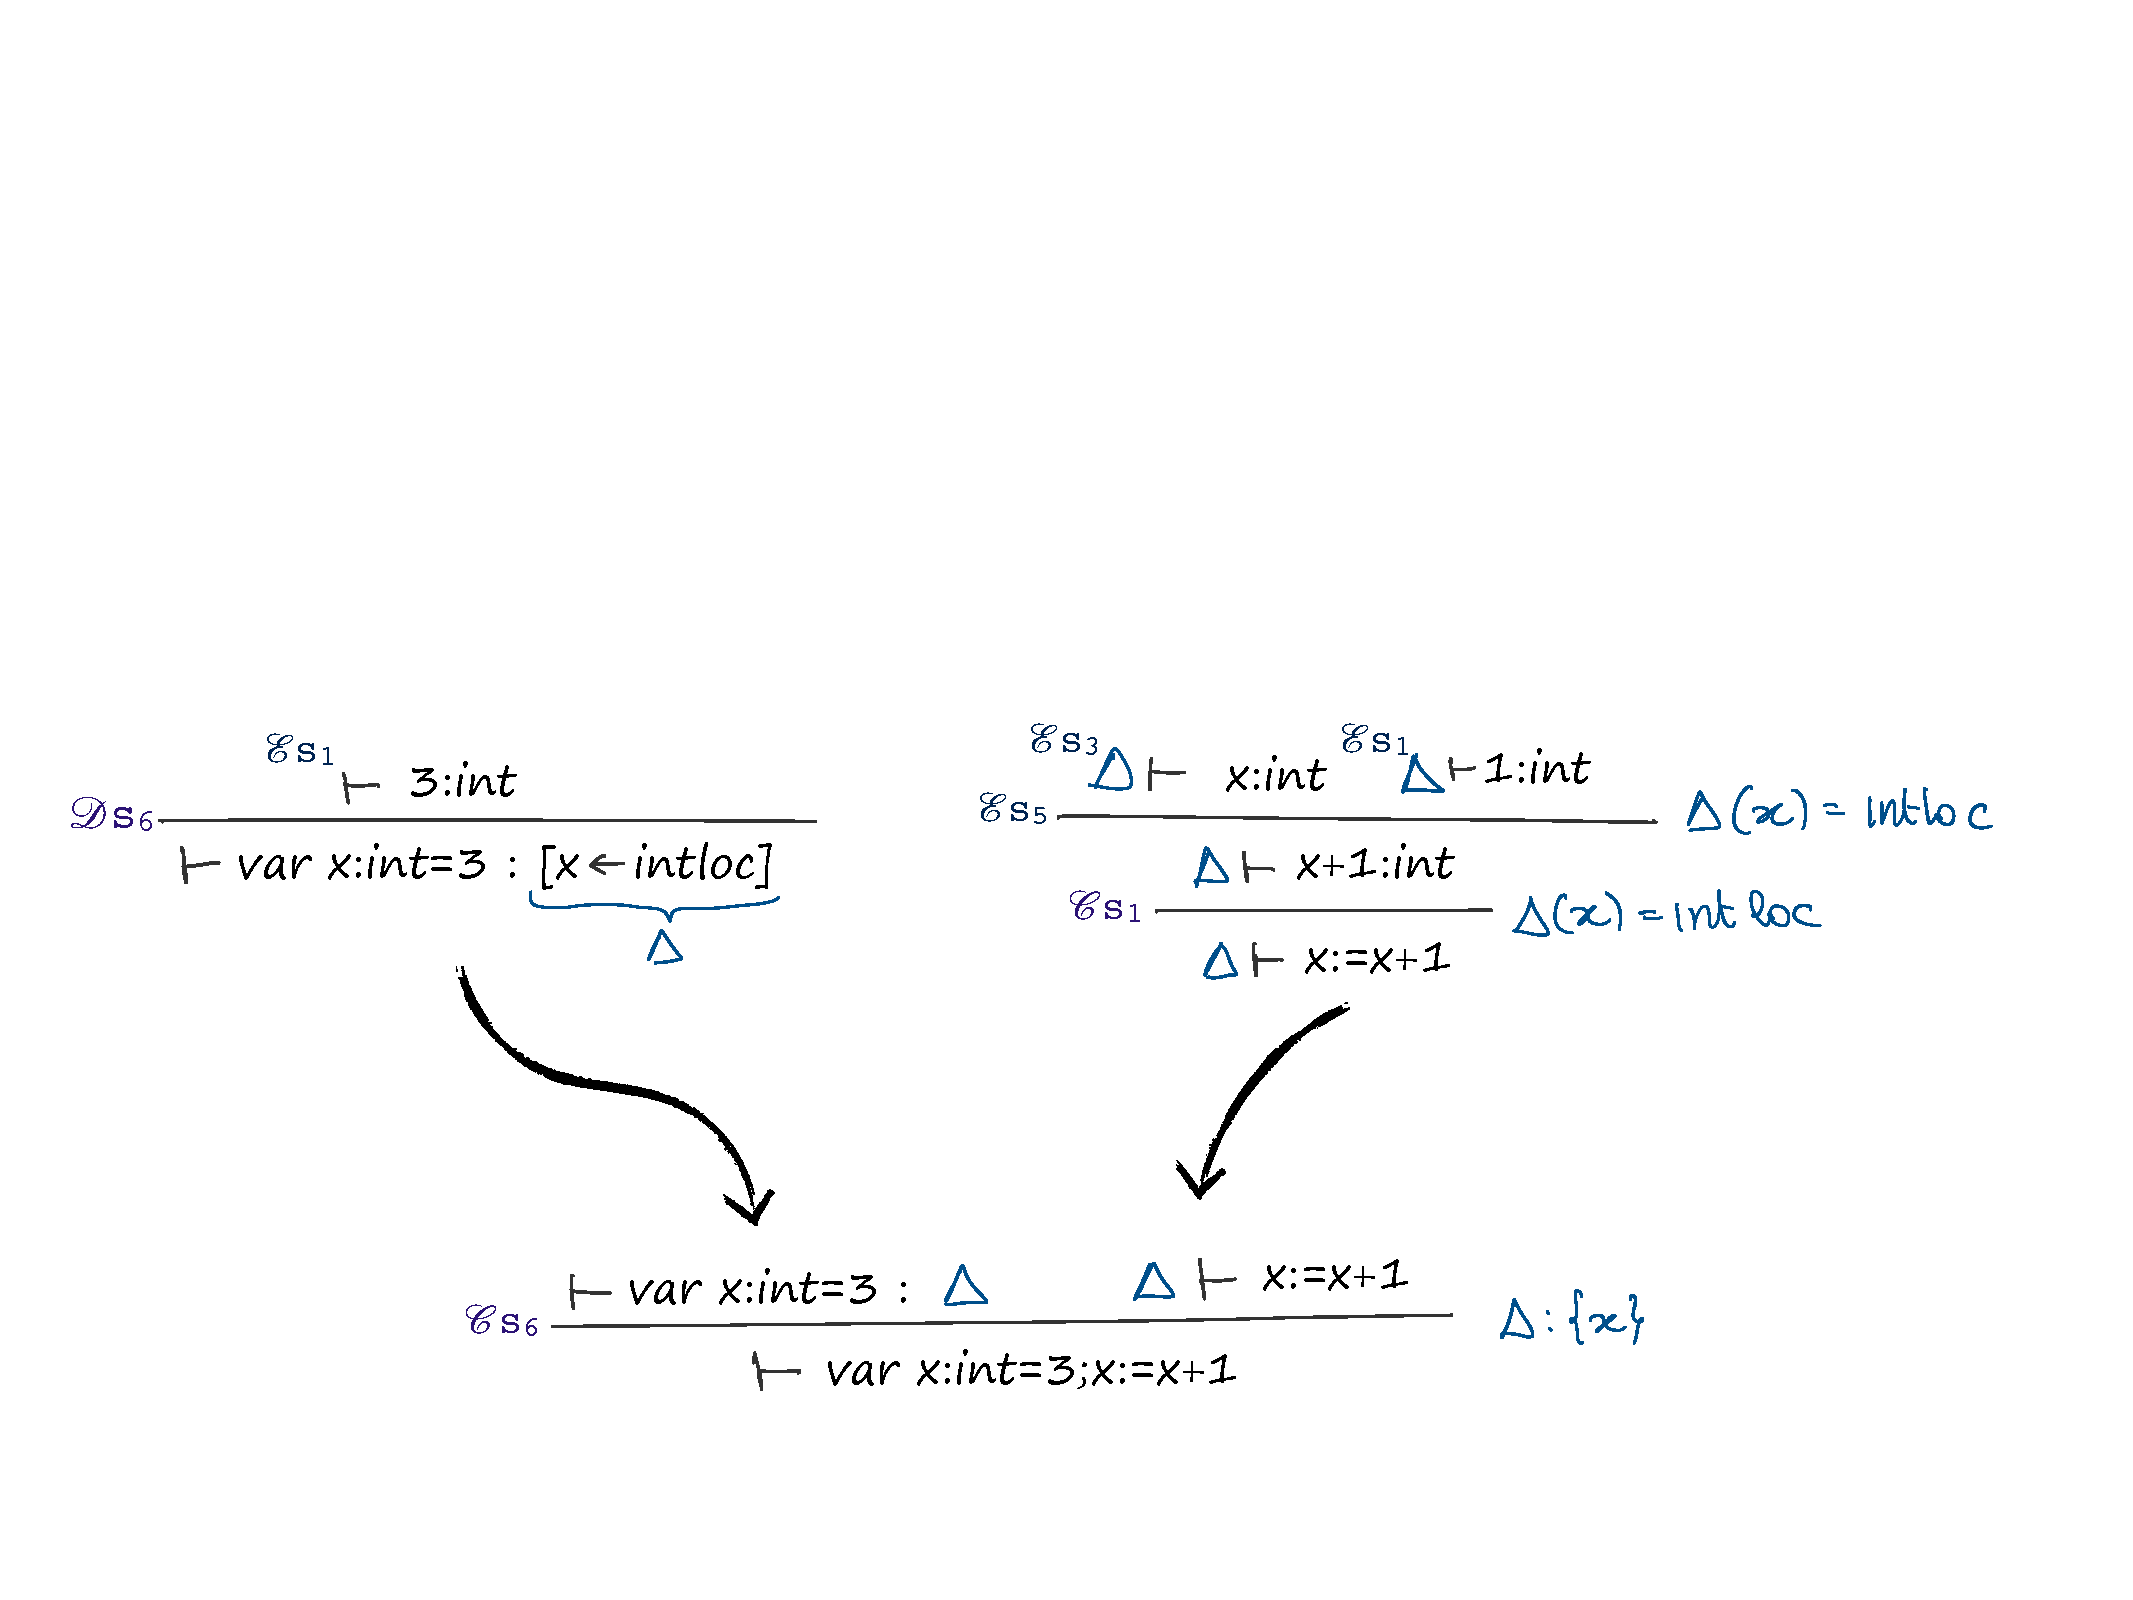
\includegraphics[width=\textwidth]{img/imp_esempio-blocchi-1.pdf}
 	\end{figure}

 	\noindent
 	E infine, la dimostrazione di semantica dinamica:
 	\begin{figure}[!htp]
 		\centering
 		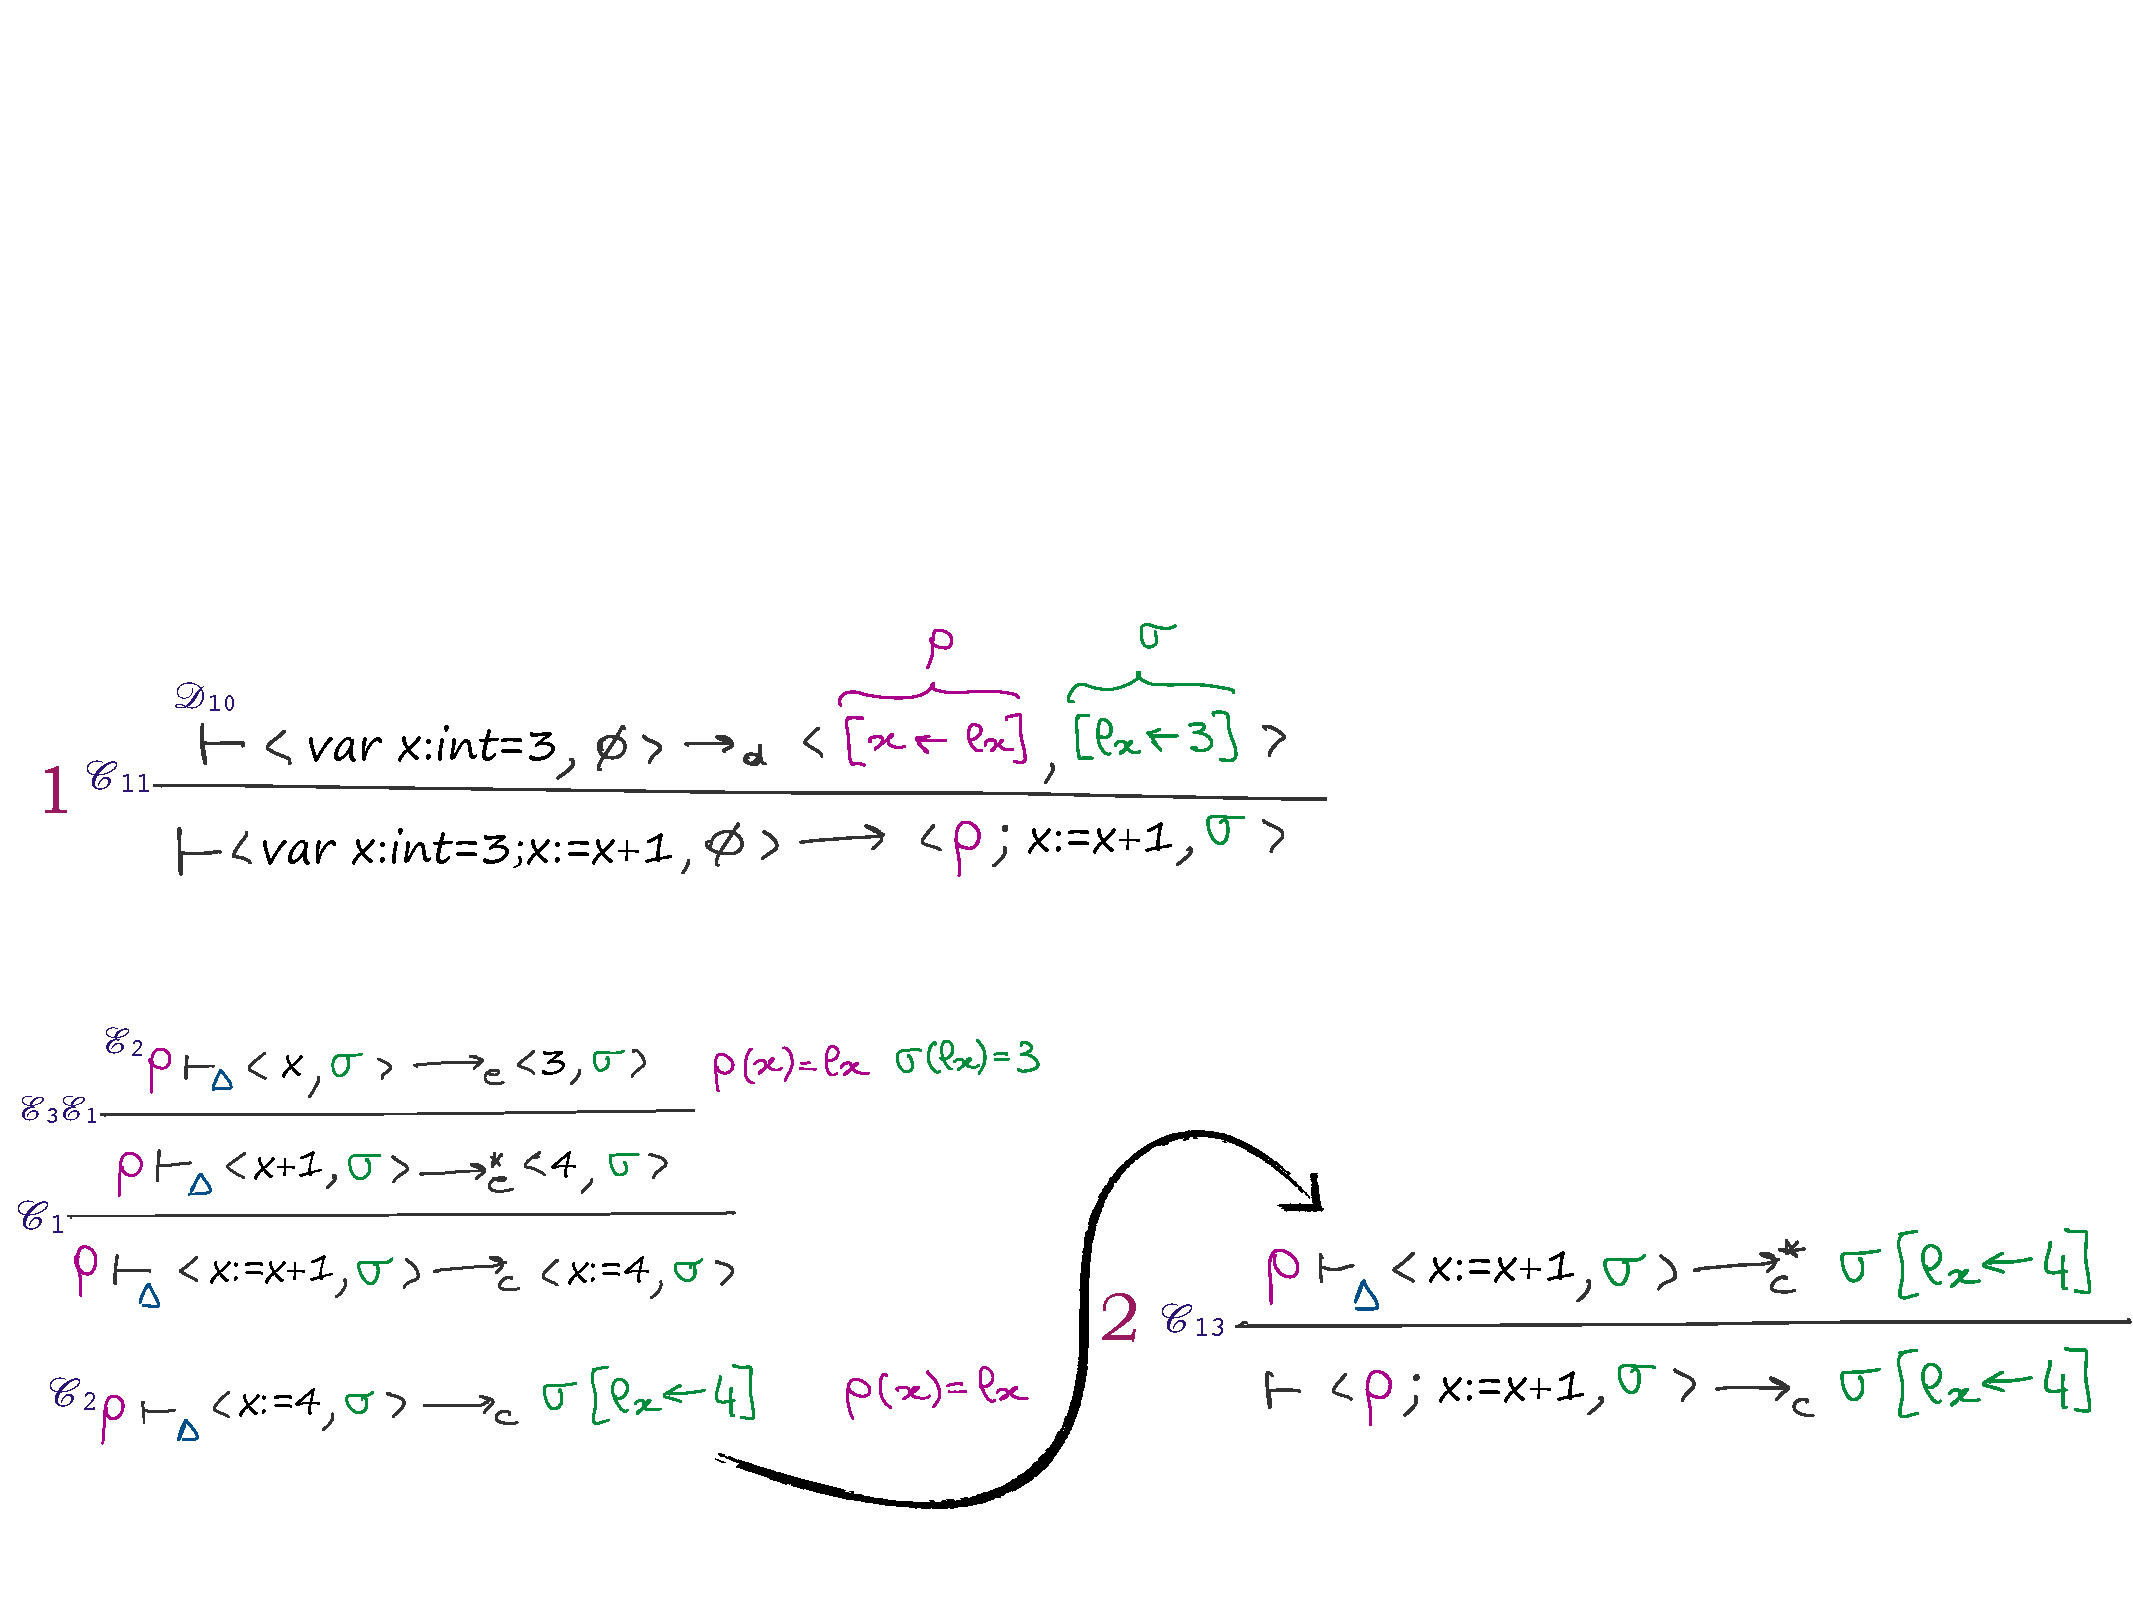
\includegraphics[width=\textwidth]{img/imp_esempio-blocchi-2.pdf}
 	\end{figure}\newpage
 	
 	\subsection{Esecuzione ed equivalenza}
 	
 	Il risultato dell'esecuzione dei comandi è una memoria (finale) con nessun altro comando da eseguire.
 	
 	\begin{boxdef}
 		L'\textcolor{Red3}{\textbf{esecuzione dei comandi}} è descritta nel seguente modo. L'elaborazione è una funzione:
 		\begin{equation*}
 			Exec: \mathcal{E}^{V} \times \mathsf{Mem} \longrightarrow \mathsf{Mem}
 		\end{equation*}
 		Che descrive il comportamento dinamico dei comandi restituendo la memoria, che rappresenta il risultato delle trasformazioni effettuate dai comandi eseguiti:
 		\begin{equation*}
 			Exec\left(\left\langle c,\sigma \right\rangle\right) = \sigma' \hspace{1em} \iff \hspace{1em} \left\langle c,\sigma \right\rangle \longrightarrow* \sigma'
 		\end{equation*}
 	\end{boxdef}
 	
 	\noindent
 	L'equivalenza ha una quantificazione universale sulle memorie iniziali, ovvero i comandi devono dare lo stesso risultato per ogni possibile memoria iniziale.
 	
 	\begin{boxdef}
 		L'\textcolor{Red3}{\textbf{equivalenza di comandi}} è descritta nel seguente modo. L'equivalenza di comandi è una relazione:
 		\begin{equation*}
 			\equiv \subseteq \mathcal{E}^{V} \times \mathcal{E}^{V}
 		\end{equation*}
 		Definita come segue:
 		\begin{equation*}
 			c_{0} \equiv c_{1} \hspace{1em} \iff \hspace{1em} \forall\sigma : Exec\left(\left\langle c_{0}, \sigma \right\rangle\right) = Exec\left(\left\langle c_{1}, \sigma \right\rangle\right)
 		\end{equation*}
 	\end{boxdef}\newpage
 	
 	\section{Procedure}
 	
 	\subsection{Astrazione del controllo}
 	
 	\subsubsection{Nomi e parametri, interfacce e corpi}
 	
 	Ogni categoria sintattica semanticamente significativa può essere utilizzata come astrazione:
 	\begin{itemize}
 		\item Le espressioni;
 		
 		\item Le dichiarazioni con i tipi di dati astratti;
 		
 		\item I comandi con le procedure, i quali sono lu strumento sintattico per l'astrazione del controllo.
 	\end{itemize}
 	La \textbf{categoria sintattica più interessante}, dal punto di vista dell'astrazione, è quella dei \textbf{comandi}. Questo perché ha come obbiettivo quello di \textbf{abbreviare la scrittura di programmi che contengono sequenze ripetute di comandi uguali}, ma che possono differire nei dati su cui operano.\newline
 	
 	\noindent
 	Le \textbf{motivazioni} per cui viene eseguita l'\textbf{astrazione} sono molteplici:
 	\begin{itemize}
 		\item Maggiore leggibilità del codice;
 		\item Utilizzo ripetuto delle stesse espressioni o gruppi di comandi;
 		\item Riduzione delle possibilità di errore.
 	\end{itemize}
 	
 	\noindent
 	Parte \textbf{fondamentale dell'astrazione} consiste nel \textbf{dare} al raggruppamento un \textcolor{Red3}{\textbf{nome}}. Infatti, l'introduzione di nomi consiste nella creazione di nuovi legami che permettano di interpretare i nomi stessi durante l'esecuzione. Per \textcolor{Green4}{\textbf{esempio}}, grazie all'uso di un nome, è possibile rappresentare un insieme di elementi complessi che vengono così trattati come un'unica entità.
 	
 	Inoltre, il \textbf{nome consente di riferirsi all'astrazione senza conoscerne i dettagli}, ma solo le caratteristiche di interesse che ne hanno determinato il raggruppamento.\newline
 	
 	\noindent
 	Per aumentare l'astrazione, vengono introdotti i \textcolor{Red3}{\textbf{parametri}}. Essi sono abbreviati con un nome e \textbf{consentono l'astrazione di tante computazioni simili}, le quali cambiano solo per alcuni input a cui vengono applicate.\newline
 	
 	\noindent
 	Unendo \emph{\textbf{nomi}} e \emph{\textbf{parametri}}, si formano le \textcolor{Red3}{\textbf{interfacce}} dell'astrazione, ovvero tutto \textbf{quello che è necessario conoscere per poter utilizzare correttamente le procedure}. Quindi, grazie alle interfacce viene reso visibile solo cosa è visibile dall'astrazione, nascondendo tutti gli altri dettagli. Vengono enfatizzate le similarità delle diverse istanze raggruppate nascondendo le differenze.\newline
 	
 	\noindent
 	Il \textcolor{Red3}{\textbf{corpo}} è \textbf{ciò che viene valutato, elaborato ed eseguito, ogni qualvolta il nome viene richiamato (con eventuali parametri) in qualche punto del programma}. Il corpo è analogo ai blocchi senza nome (par.~\ref{blocchi}), ovvero incapsula una sequenza di comandi in un'interfaccia.\newpage
 	
 	\subsubsection{Funzioni e procedure}
 	
 	Durante l'astrazione esistono due tipologie di categorie di \textbf{sottoprogrammi} con nome che possono essere definite:
 	\begin{itemize}
 		\item Le \textbf{\emph{procedure}} sono collezioni di comandi che definiscono una computazione parametrizzata.\newline
 		Le procedure sono ogni forma di astrazione di comandi che ha un nome e non viene necessariamente restituito un risultato. L'\textbf{obbiettivo principale è che eseguano una modifica di stato}.
 		
 		\item Le \textbf{\emph{funzioni}} sono strutturalmente simili alle procedure ma semanticamente sono modellate come le classiche funzioni.\newline
 		Le funzioni, a differenza delle procedure, eseguono sia una modifica di stato sia una modifica di stato. Inoltre, talvolta è possibile che venga prodotto \href{https://en.m.wikipedia.org/wiki/Side_effect_(computer_science)}{\emph{side effects}}.
 	\end{itemize}
 	Indipendentemente dall'invocazione di una funzione o una procedura, è possibile ignorare o considerare i cambiamenti di stato:
 	\begin{itemize}
 		\item Il \textbf{chiamante} (chi invoca la funzione/procedura) \textbf{ignora i cambiamenti di stato intermedi} e tiene solo lo stato di chiamata che passa allo stato di ritorno;
 		
 		\item Il \textbf{chiamante utilizza l'intero codice presente all'interno della funzione/procedura}. In questo caso, il chiamante è interessante a tutti i cambiamenti di stato intermedi.
 	\end{itemize}
 	
 	\noindent
 	\begin{boxdef}
 		Un \textcolor{Red3}{\textbf{sottoprogramma}} è un concetto base (funzione o procedura), porzione di codice identificato da un nome, dotato di un ambiente locale proprio e capace di scambiare informazioni con il resto del codice mediante fissati canali (parametri e/o valori di ritorno)
 	\end{boxdef}
 	
 	\noindent
 	La caratterizzazione di un sottoprogramma si basa sulla specifica, sulla definizione (scrittura vera e propria) e sulla chiamata (è necessario utilizzarlo). Il tutto viene fatto senza conoscerne il contesto. Quindi la sequenza è la seguente:
 	\begin{enumerate}
 		\item \textbf{Specifica} del sottoprogramma;
 		\item \textbf{Scrittura} del sottoprogramma;
 		\item \textbf{Utilizzo} del sottoprogramma.
 	\end{enumerate}\newpage
 	
 	\subsection{Visibilità con le procedure e ambienti di riferimento}
 	
 	Ricordando la regola di visibilità enunciata a pagina~\pageref{regola di visibilità}, essa è possibile estenderla alle procedure grazie al concetto di ambienti di riferimento per un comando:
 	\begin{boxdef}
 		L'\textcolor{Red3}{\textbf{ambiente di riferimento}} di un comando è la collezione di tutti i nomi che sono visibili al comando.
 	\end{boxdef}
 	
 	\noindent
 	L'ambiente di riferimento di una procedura è determinato da varie tipologie di regole:
 	\begin{itemize}
 		\item Regole di \textbf{scope} (statico o dinamico);
 		
 		\item Regole \textbf{specifiche}, per esempio quando è visibile una dichiarazione nel blocco in cui compare;
 		
 		\item Regole per il \textbf{passaggio dei parametri};
 		
 		\item Regole di \textbf{binding} (\emph{shallow} o \emph{deep}) che intervengono quando una procedura è passata come parametro ad un'altra procedura.
 	\end{itemize}
 	In particolare, \textbf{le regole di scope e di binding servono esclusivamente quando la procedura contiene un ambiente non locale}.\newpage
 	
 	\subsection{Scope statico e dinamico}
 	
 	Esistono due tipologie di scope:
 	\begin{itemize}\label{scope statico e dinamico}
 		\item \textbf{Scope statico}, dove gli \textbf{identificatori} liberi della procedura (cioè ambiente non locale), sono \textbf{\underline{staticamente} legali all'ambiente}, quindi a \textbf{tempo di compilazione}.
 		
 		Lo scope statico si basa esclusivamente sul testo del codice, e lega l'identificatore al blocco che lessicalmente lo contiene, ovvero in cui è stato dichiarato.
 		
 		\begin{boxdef}
 			Nello \textcolor{Red3}{\textbf{scope statico}} un nome non locale è risolto nel blocco che testualmente lo racchiude.
 		\end{boxdef}
 		
 		\item \textbf{Scope dinamico}, i \textbf{legami} \underline{non} sono creati a tempo di esecuzione, ma è necessario \textbf{eseguire il programma per individuarli} e \textbf{quindi i legami stessi sono dinamici}. In altre parole, viene presa in considerazione l'ultima chiamata aperta e non ancora chiusa in cui la variabile è stata definita.
 		
 		Diverse chiamate alla stessa procedura possono essere eseguite in ambienti diversi, quindi gli stessi oggetti possono essere risolti con legami differenti.
 		
 		\begin{boxdef}
 			Nello \textcolor{Red3}{\textbf{scope dinamico}} un nome non locale è risolto nella chiamata attivata più di recente e non ancora terminata.
 		\end{boxdef}
 	\end{itemize}
 	Per esempio, dato il seguente codice:
 	\lstinputlisting[language=C]{code/scope-statico_dinamico.c}
 	La chiamata \textsf{write(x);} a riga 11, con scope statico stampa 0, mentre con scope dinamico stampa 4.\newpage
 	
 	\subsubsection{Scope statico}
 	
 	Lo scope statico ha alcuni aspetti che lo caratterizzano:
 	\begin{itemize}
 		\item \textbf{Garantisce l'indipendenza del risultato della procedura dalla posizione}. Per \textcolor{Green4}{\textbf{esempio}}, si consideri il seguente codice:
 		\lstinputlisting[language=C]{code/scope_statico-ex1.c}
 		Il corpo della funzione \textsf{foo} è parte dello scope della \textsf{x} più esterna. Invece, la chiamata della funzione \textsf{foo} è compresa nello scope della \textsf{x} più interna. Nonostante \textsf{foo} possa essere chiamata in molti contesti diversi, lo scope statico è l'unico in cui essa può essere compilata in modo univoco. Facendo sempre riferimento alla \textsf{x} più esterna.
 		
 		Ovviamente, la visibilità di una dichiarazione varia a seconda delle regole fissate dal linguaggio.
 		
 		\item (\underline{svantaggio}) \textbf{Necessita di più accessi}, rispetto al necessario, a variabili e sottoprogrammi;
 		
 		\item (\underline{svantaggio}) I \textbf{sottoprogrammi diventano globali} poiché utilizzano variabili esterne.
 	\end{itemize}
 	Un \textcolor{Green4}{\textbf{esempio}} di codice scritto in Javascript:
 	\lstinputlisting[language=JavaScript]{code/scope_statico-ex2.js}
 	I valori stampati sono: 12 47. Quindi, la funzione \textsf{addn()} utilizza il valore 17, ma questo non indica che il linguaggio utilizzi lo scope dinamico. Infatti, nella seconda dichiarazione di \textsf{n} (riga 8), non vi è un blocco ma semplicemente una sovrascrizione della prima dichiarazione di \textsf{n} (riga 1).\newpage
 	
 	\noindent
 	È possibile osservare quale tipo di scope è utilizzato con il seguente codice:
 	\lstinputlisting[language=JavaScript]{code/scope_statico-ex3.js}
 	In questo caso il risultato è: 42 12. La chiamata \textsf{addn()} (riga 9) usa la prima dichiarazione di \textsf{n} (riga 1). Nel caso in cui si decommenti la riga 13, il risultato sarebbe: 43 13. \newline
 	
 	\noindent
 	Un altro \textcolor{Green4}{\textbf{esempio}} di codice scritto in Python:
 	\lstinputlisting[language=Python]{code/scope_statico-ex4.py}
 	Anche in questo caso il risultato è: 42 12. Quindi, la funzione \textsf{addn()} utilizza il valore 12. Nel caso in cui venga decommentata la riga 11, il risultato sarebbe: 43 13.\newline
 	
 	\noindent
 	Considerando un altro esempio in Python:
 	\lstinputlisting[language=Python]{code/scope_statico-ex5.py}
 	In questo caso il risultato è: 17 4. Alla riga 9 viene invocata la funzione \textsf{f} con parametro \textsf{z} che corrisponde a 3; la \textsf{x} a riga 9 è uguale a 5; la moltiplicazione a riga 5 è 12 poiché viene presa la variabile \textsf{x} esterna.\newpage
 	
 	\subsubsection{Scope dinamico}
 	
 	Lo scope dinamico ha alcune caratteristiche:
 	\begin{itemize}
 		\item È \textbf{basato sulla sequenza di chiamate del programma}, e non sulla struttura del codice. Quindi, un nome non locale viene risolto nella chiamata attivata più recente e non ancora disattivata;
 		
 		\item (\underline{vantaggio}) \textbf{Convenienza};
 		
 		\item (\underline{svantaggio}) Durante l'esecuzione del programma, le sue \textbf{variabili sono visibili a tutti i sottoprogrammi che invoca};
 		
 		\item (\underline{svantaggio}) Il \textbf{riferimento di una variabile} in un punto del programma \textbf{può variare a seconda dell'esecuzione};
 		
 		\item (\underline{svantaggio}) \textbf{Impossibile eseguire una verifica statica};
 		
 		\item (\underline{svantaggio}) \textbf{Ridotta leggibilità}, ovvero non è possibile determinare staticamente (punto precedente) il tipo di una variabile.
 	\end{itemize}
 	Per i vari svantaggi, il tipo dinamico viene utilizzato meno dello statico.\newline
 	
 	\noindent
 	Il seguente \textcolor{Green4}{\textbf{esempio}} riporta un codice nel linguaggio di programmazione Perl:
 	\lstinputlisting[language=Perl]{code/scope_dinamico-ex1.pl}
 	Il risultato visualizzato è: 47 47. Infatti, la dichiarazione dentro la funzione \textsf{set()} è globale, quindi lo scope non interviene. Per eseguire la verifica e capire quale scope viene utilizzato, è necessario dichiarare una variabile locale in \textsf{set()}. Dunque, scrivendo alla riga 8 il comando \dquotes{\textsf{local \$n = 17;}} è possibile notare che lo scope è dinamico. Il risultato muta in 47 12, quindi la chiamata \textsf{addn()} utilizza la dichiarazione \dquotes{\textsf{local \$n = 17;}} (riga 8) valida al momento delle chiamata della funzione \textsf{addn()}. Invece, esternamente il valore di \textsf{n} rimane 12.\newpage
 	
 	\subsubsection{Sintesi}
 	Lo \textbf{scope statico} è quando un nome non locale è risolto nel blocco che testualmente lo racchiude. In questo caso, le associazioni sono note a tempo di compilazione. L'implementazione è complessa ma risulta molto efficiente e soddisfa i principi di indipendenza.\newline
 	
 	\noindent
 	Lo \textbf{scope dinamico} è quando un nome non locale è risolto nella chiamata attivata più di recente e non ancora disattiva. In questo caso, l'informazione è derivata dall'esecuzione e causa programmi meno leggibili. Facile da implementare ma poco efficiente.\newline
 	
 	\noindent
 	N.B. \textbf{Se non ci sono procedure, o se nelle precedure non c'è un ambiente non locale (o se c'è ma è incluso nell'ambiente globale) allora non ha senso distinguere i due metodi, in quanto il risultato sarebbe sempre lo stesso.} Quindi i due metodi di scope differiscono solo nel contesto delle procedure con presenza congiunta di ambiente non locale e non globale.\newpage
 	
 	\subsection{Allocazione della memoria}
 	Un concetto fondamentale legato all'uso delle procedure è l'\textbf{allocazione della memoria}, ovvero come vengono allocati gli oggetti e dove vengono risolti i riferimenti (non locali). Anche in questo caso, l'allocazione di memoria si divide in \textbf{due tipi}:
	\begin{itemize}
		\item \textcolor{Red3}{\textbf{Statica}}, la \textbf{memoria allocata} a \textbf{tempo di compilazione}. Quindi, prima dell'esecuzione, i dati del programma vengono disposti in zone di memoria dove rimangono fino alla fine;
		
		\item \textcolor{Red3}{\textbf{Dinamica}}, la \textbf{memoria allocata} a \textbf{tempo di esecuzione}. Quindi, vengono utilizzate delle strutture dinamiche:
		\begin{itemize}
			\item \textbf{Pila} (\textbf{stack}), gli oggetti vengono allocati con la politica LIFO;
			
			\item \textbf{Heap}, gli oggetti vengono allocati e deallocati in qualsiasi momento.
		\end{itemize}
		Le quali durante l'esecuzione vengono continuamente allocale e deallocate.
	\end{itemize}
	
	\longline
 	
 	\subsubsection{Allocazione statica}
 	
 	L'\textbf{allocazione statica} consente di \textbf{allocare} lo spazio per tutti gli identificatori a \textbf{tempo di compilazione}. Questo metodo comporta una serie di \textbf{caratteristiche}:
 	\begin{itemize}
 		\item La \textbf{memoria rimane allocata per l'intera esecuzione};
 		
 		\item Il \textbf{tempo di vita} di tutti gli \textbf{identificatori} è pari al tempo dell'\textbf{esecuzione dell'intero programma};
 		
 		\item \textbf{Necessario conoscere a priori quanta memoria è necessaria};
 		
 		\item \textbf{Impossibile eseguire la ricorsione} poiché non è possibile stabilire a priori quante volte verrà ripetuta (\underline{limite più importante dell'allocazione statica});
 		
 		\item \textbf{Impossibile avere blocchi annidati} poiché i riferimenti sono puramente statici;
 		
 		\item \textbf{Ogni oggetto ha un indirizzo assoluto che viene mantenuto per tutta l'esecuzione del programma};
 	\end{itemize}
 	Le allocazioni statiche sono eseguite su:
 	\begin{itemize}
 		\item Variabili globali;
 		\item Variabili locali nei sottoprogrammi (senza ricorsione);
 		\item Costanti determinabili a tempo di compilazione;
 		\item Tabelle usate dal supporto a run-time (e.g. \emph{garbage collection})
 	\end{itemize}
 	\textcolor{Green4}{\textbf{Esempi}} di linguaggi che utilizzano l'allocazione statica sono COBOL e FORTRAN.\newline
 	
 	\noindent
 	Nonostante le caratteristiche apparentemente negative, l'allocazione statica consente \textbf{esecuzioni più veloci} poiché è possibile utilizzare indirizzi assoluti e quindi il dato si troverà sempre nella stessa posizione.\newpage
 	
 	\subsubsection{Allocazione dinamica}
 	L'\textbf{allocazione dinamica} supera i limiti imposti dall'allocazione statica e consente di creare \textcolor{Red3}{\textbf{record di attivazione}} (\textbf{RdA} o \textbf{frame}), per ogni istanza di un sottoprogramma a run-time, contenente le informazioni relative a tale istanza. La struttura dati preferita per gestire i record di attivazione è la \textcolor{Red3}{\textbf{pila (stack)}}, poiché consente di implementare la struttura a blocchi dei programmi\footnote{Si intende, per esempio, che una volta entrati in A e poi in B, è necessario prima uscire da B e solo dopo da A.}.\newline
 	
 	\noindent
 	Le caratteristiche positive e negative sono:
 	\begin{itemize}
 		\item \textbf{Consente la ricorsione};
 		\item \textbf{Aumento dell'overhead} per allocazione e deallocazione effettuata, questo comporta un'\textbf{esecuzione più lenta};
 	\end{itemize}
 	
 	\longline
 	
 	\subsubsection{Record di attivazione}
 	
 	La pila viene gestita eseguendo una serie di operazioni:
 	\begin{itemize}
 		\item Sequenza di chiamata;
 		\item Prologo;
 		\item Epilogo;
 		\item Sequenza di ritorno.
 	\end{itemize}
 	Inoltre, dato che l'indirizzo viene calcolato a tempo di esecuzione, la sua \textbf{gestione} viene effettuata \textbf{tramite un puntatore} RdA, chiamato \textbf{Stack Pointer} (SP), il quale \textbf{punta} al Record di Attivazione del blocco attivo, ovvero quello \textbf{in cima allo stack}.\newline
 	
 	\noindent
 	Le \textbf{informazioni contenute all'interno dei Record di Attivazione} sono accessibili tramite l'uso dello Stack Pointer in combinazione con l'\emph{offset} (determinato staticamente). Queste informazioni sono:
 	\begin{itemize}
 		\item \textbf{Link di controllo}, ovvero puntatori che puntano ai Record di Attivazione precedenti nella catena;
 		
 		\item \textbf{Indirizzo di ritorno}, ovvero l'indirizzo dell'istruzione da eseguire al termine della procedura;
 		
 		\item \textbf{Indirizzo del risultato}, ovvero l'indirizzo dove depositare il risultato della procedura se presente;
 		
 		\item \textbf{Parametri attuali della funzione}, ovvero i valori passati come input alla procedura;
 		
 		\item \textbf{Risultati intermedi}, valori calcolati durante l'esecuzione della procedura chiamata.
 	\end{itemize}\newpage
 	
 	\begin{figure}[!htp]
 		\centering
 		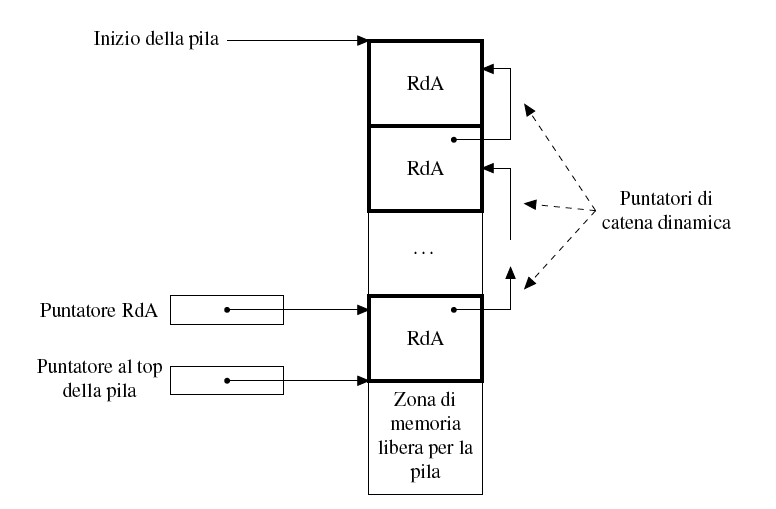
\includegraphics[width=\textwidth]{img/record_di_attivazione.png}
 		\caption{Struttura di un record di attivazione.}
 	\end{figure}
 	
 	\longline
 	
 	\subsection{Semantica delle chiamate}\label{semantica delle chiamate}
 	
 	La \textcolor{Red3}{\textbf{semantica delle chiamate}} \textbf{ad un sottoprogramma} si basa su \textbf{vari passi} che vanno implementati:
 	\begin{itemize}
 		\item \textbf{Metodi di passaggio di parametri};
 		
 		\item \textbf{Allocazione dinamico} sullo stack delle variabili locali;
 		
 		\item \textbf{Salvataggio dello stato di esecuzione} del programma chiamante;
 		
 		\item \textbf{Trasferimento del controllo} e \textbf{preparazione del ritorno};
 		
 		\item Se è supportato l'annidamento di sottoprogrammi, deve essere \textbf{gestito l'accesso a variabili non locali}.
 	\end{itemize}
 	Anche la \textcolor{Red3}{\textbf{semantica del ritorno}} \textbf{da un sottoprogramma} si basa sull'implementazione di vari passi:
 	\begin{itemize}
 		\item I \textbf{parametri} per valore e per valore-risultato \textbf{devono restituire il loro valore};
 		
 		\item \textbf{Deallocazione dello stack} per le variabili non locali;
 		
 		\item \textbf{Recupero dello stato di esecuzione} del chiamante;
 		
 		\item \textbf{Ritorno del controllo} al chiamante.
 	\end{itemize}
 	Inoltre, l'\textbf{insieme dei link dinamici presenti nello stack e validi in ogni punto di esecuzione}, viene chiamato \textcolor{Red3}{\textbf{catena dinamica}}.\newline
 	
 	\noindent
 	Infine, è possibile accedere alle variabili locali, presenti dentro i Record di Attivazione, attraverso il loro \emph{offset} (chiamato anche \emph{local\_offset}) dall'inizio del RdA.\newline
 	
 	\noindent
 	Un \textcolor{Green4}{\textbf{esempio}} di codice in cui la funzione \textsf{main} invoca \textsf{fun1}, la quale invoca \textsf{fun2}, la quale invoca \textsf{fun3}:
	\begin{lstlisting}[language=C]
void fun1(float r) {
	int s, t;
	...
	fun2(s);
	...
}
void fun2(int x) {
	int y;
	...
	fun3(y);
	...
}
void fun3(int q) {
	...
}
void main() {
	float p;
	...
	fun1(p);
	...
}\end{lstlisting}
	\begin{figure}[!htp]
		\centering
		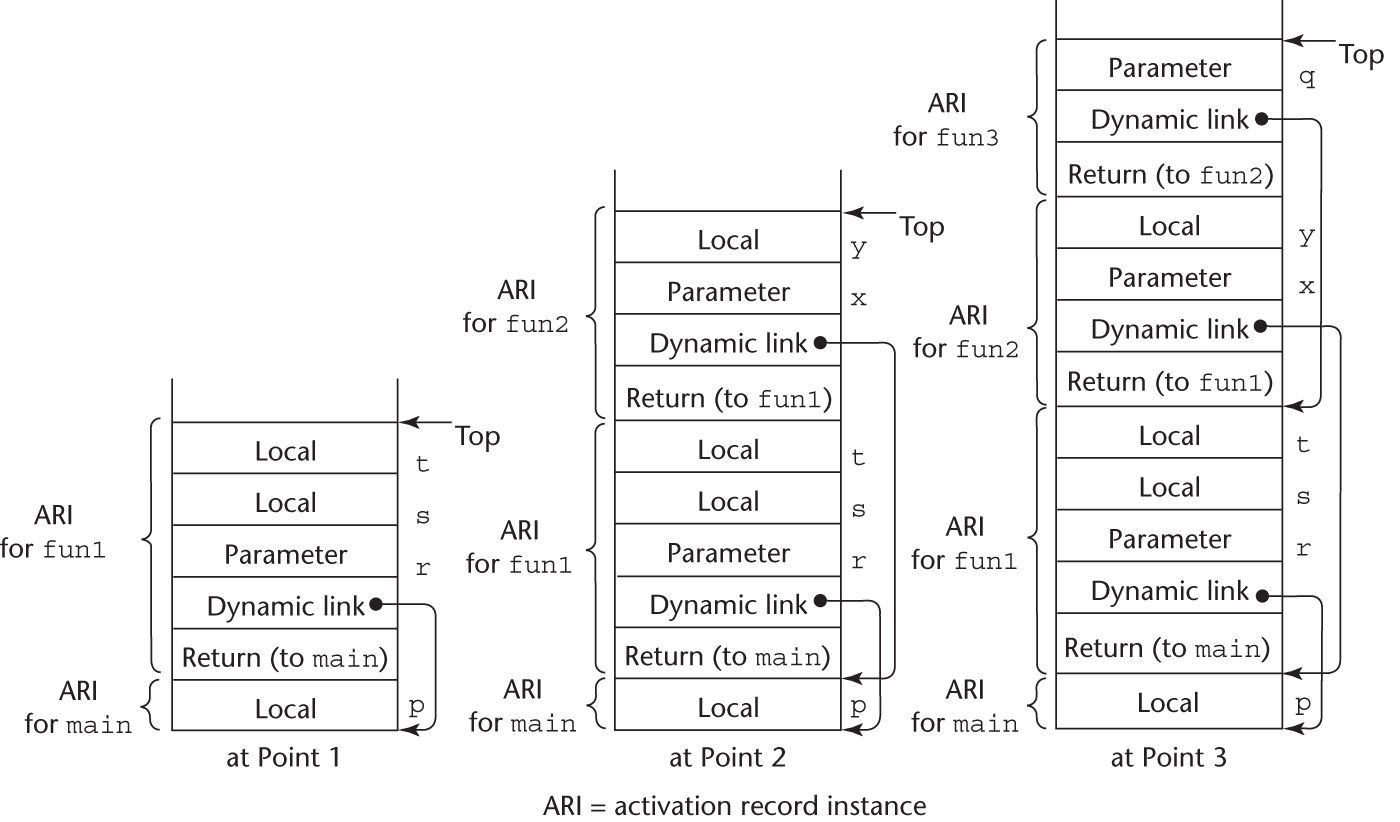
\includegraphics[width=\textwidth]{img/eg-allocazione_memoria.png}
		\caption{Stato della memoria nel tempo.}
	\end{figure}\newpage
	
	\noindent
	Qui di seguito, viene presentato invece un \textcolor{Green4}{\textbf{esempio}} tenendo in considerazione la ricorsione:
	\begin{lstlisting}[language=C]
int factorial (int n) {
	// punto 1
	if (n <= 1) return 1;
	else return (n * factorial(n - 1));
	// punto 2
}
void main() {
	int value;
	value = factorial(3);
	// punto 3
}\end{lstlisting}
	\begin{figure}[!htp]
		\centering
		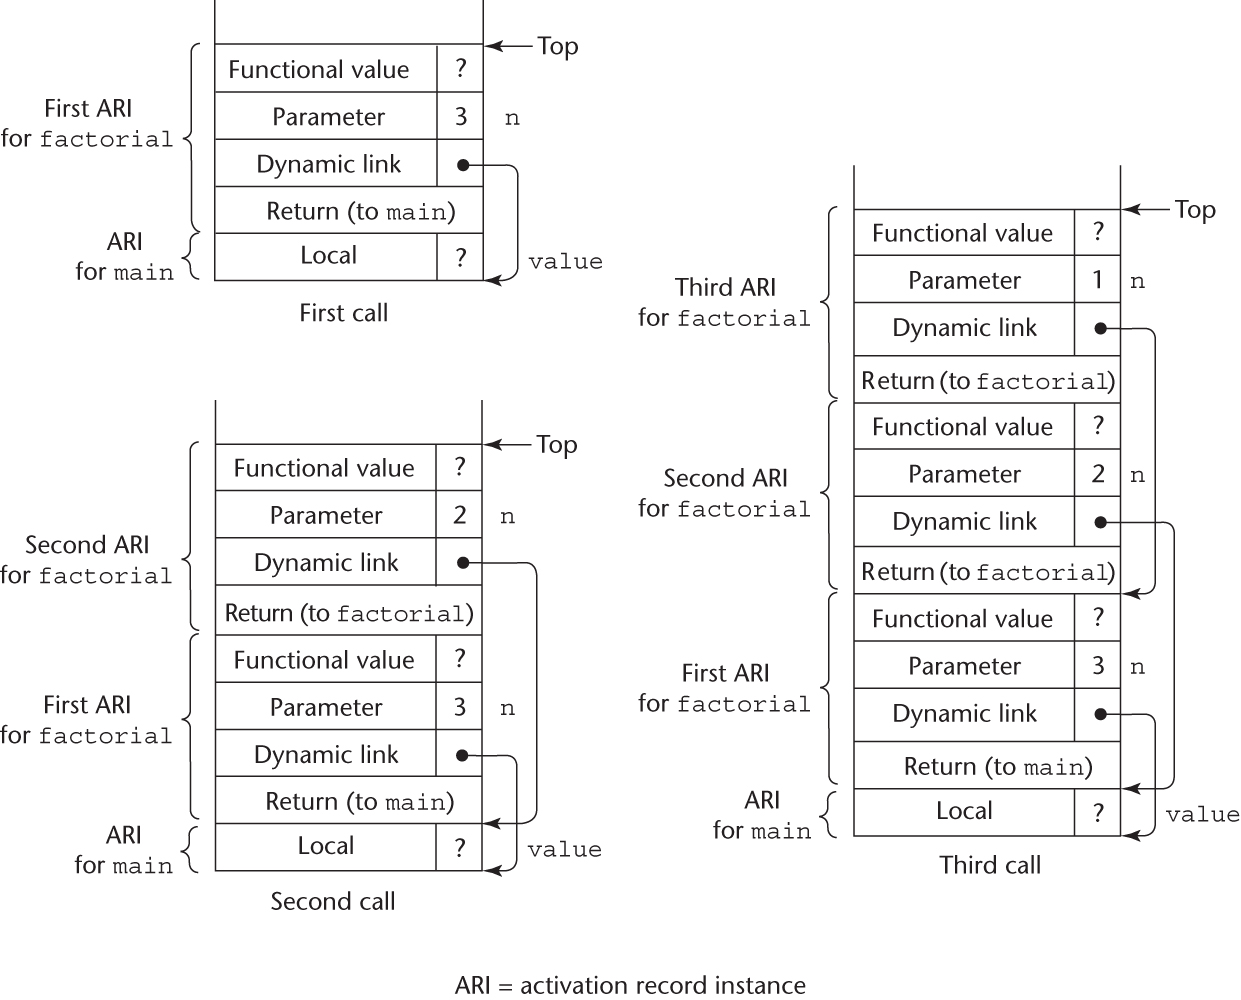
\includegraphics[width=\textwidth]{img/eg-allocazione_memoria-1.png}
		\caption{Evoluzione della Pila dopo ogni chiamata, quindi fase di chiamata.}
	\end{figure}\newpage
	
	\begin{figure}[!htp]
		\centering
		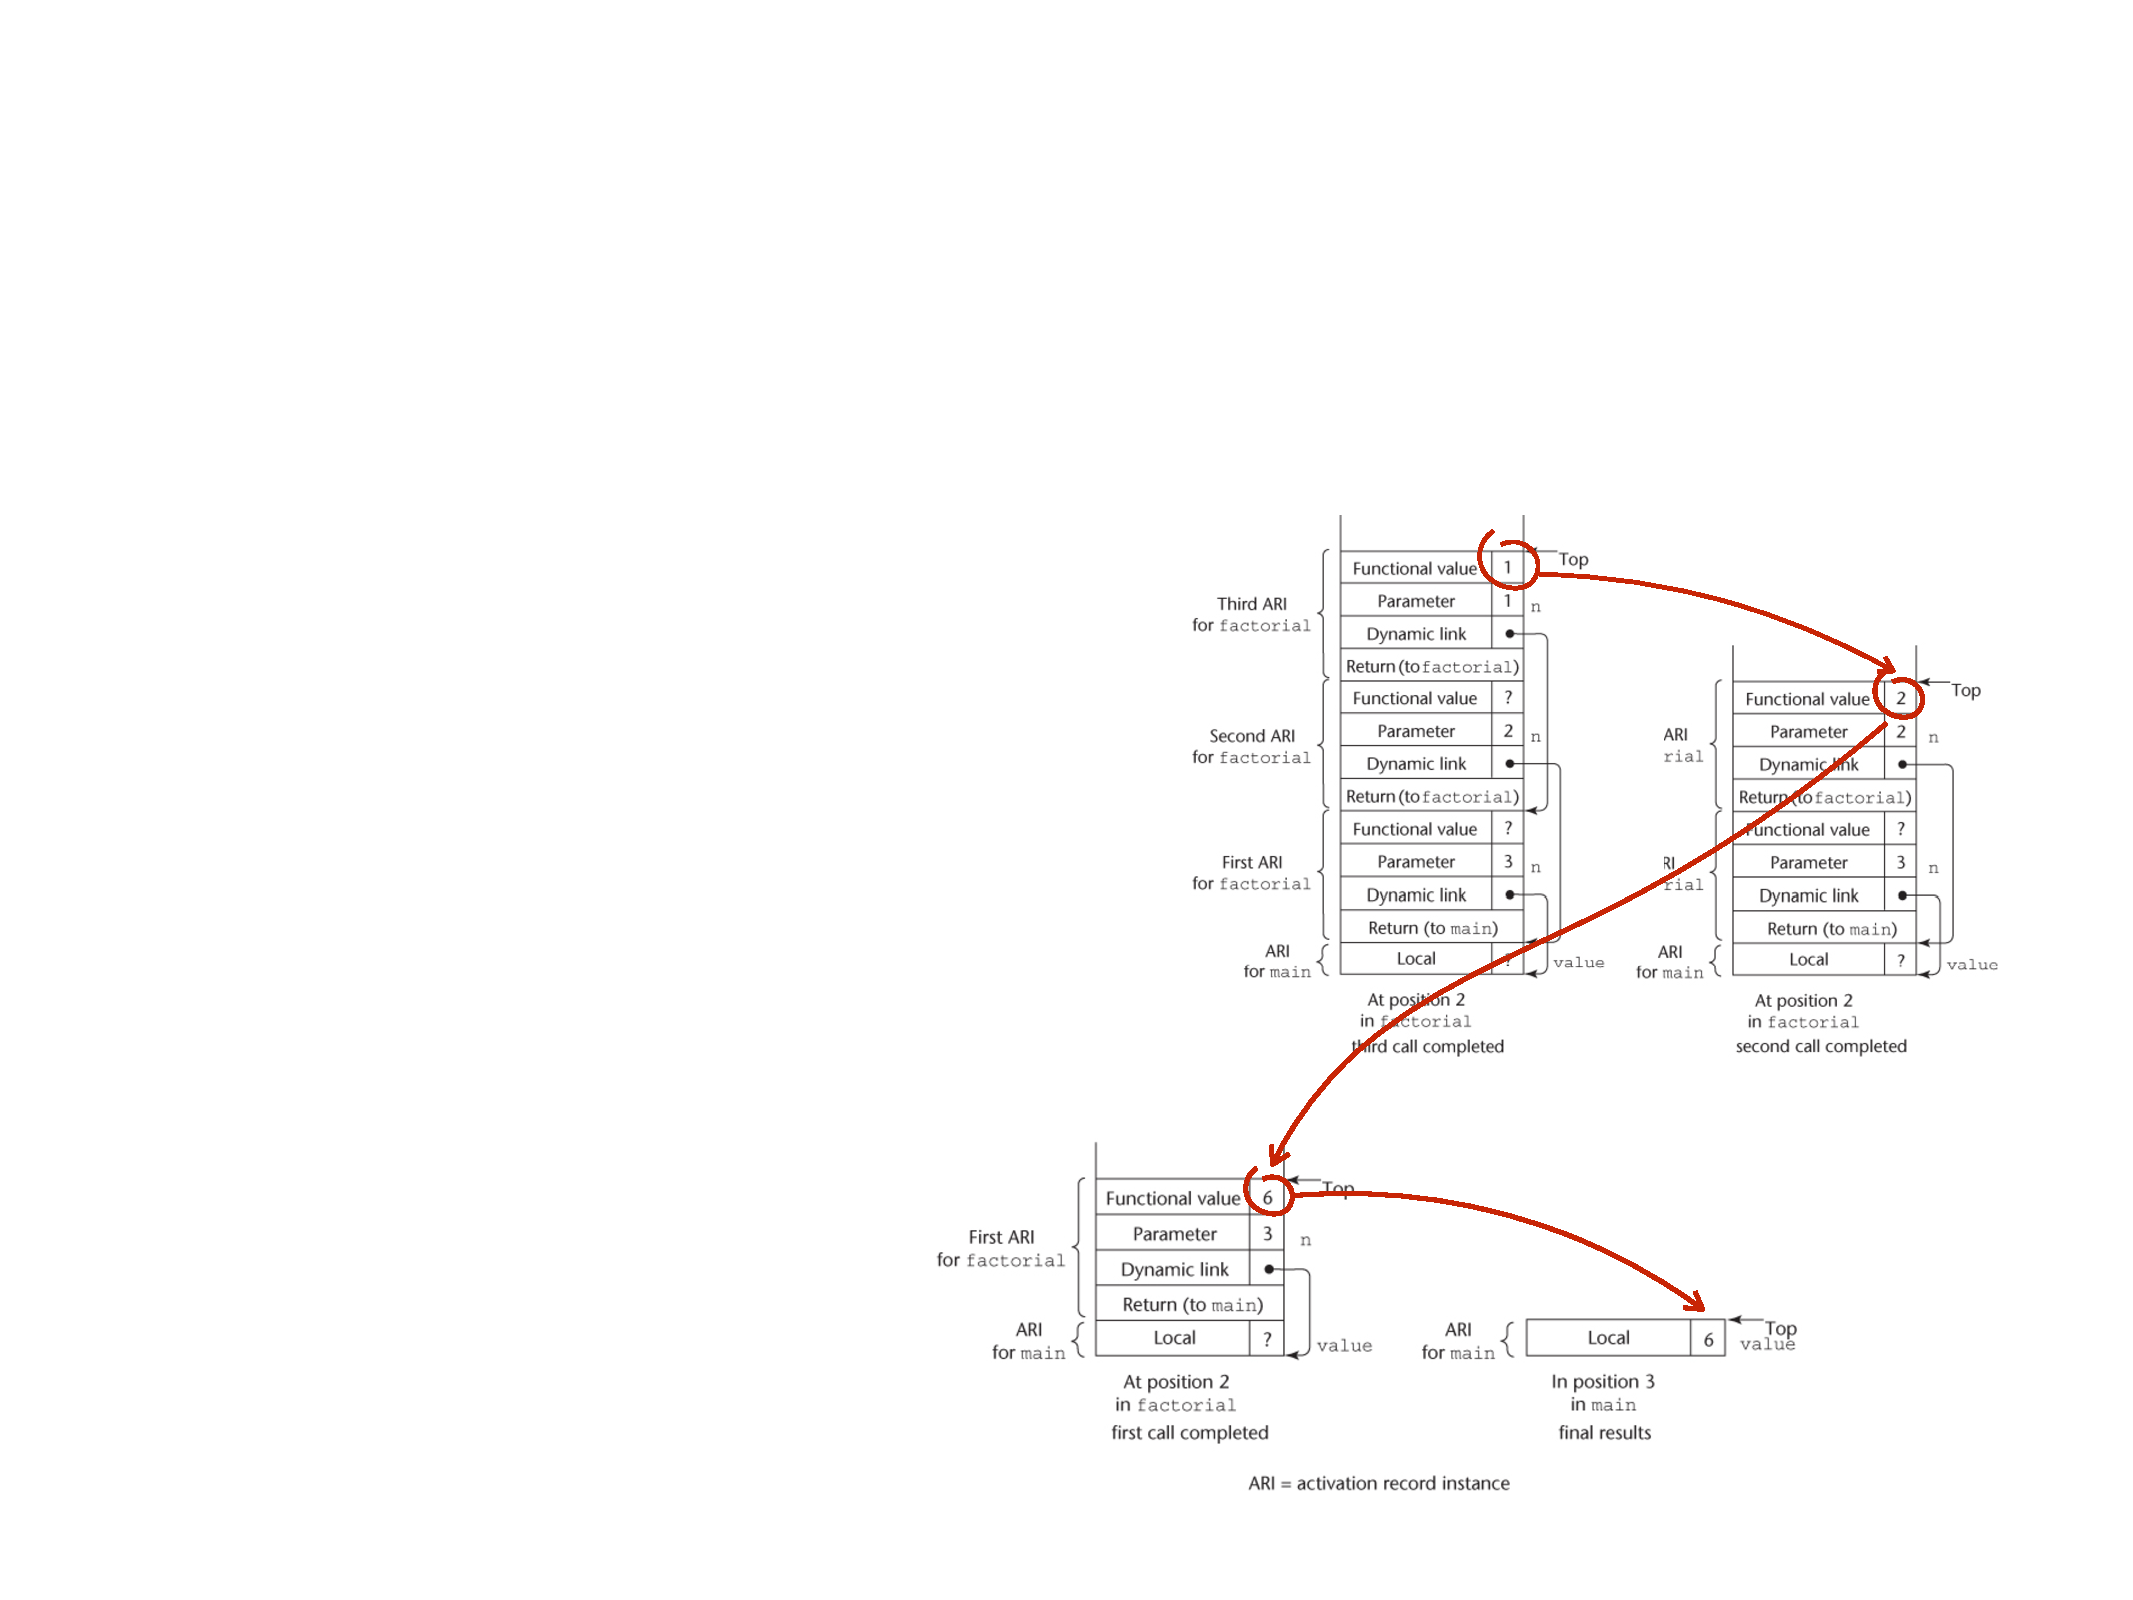
\includegraphics[width=\textwidth]{img/eg-allocazione_memoria-2.pdf}
		\caption{Evoluzione della pila dopo aver effettuato tutte le chiamate, quindi fase di ritorno.}
	\end{figure}\newpage
	
	\subsection{Implementare lo scope statico}
	
	L'\textcolor{Red3}{\textbf{implementazione dello scope statico}} è realizzabile tramite due tecniche:
	\begin{enumerate}
		\item La \textcolor{Red3}{\textbf{catena statica}} (approfondita);
		\item Il display (non trattato).
	\end{enumerate}
	Si ricorda che il Record di Attivazione possiede due link in testa: uno dinamico (spiegato nel paragrafo~\ref{semantica delle chiamate}) e uno statico. Il \textbf{link statico} è un \textbf{puntatore}, al Record di Attivazione, \textbf{del blocco che contiene il testo della parte in esecuzione}. Al contrario del link dinamico che dipende dalla sequenza di esecuzione del programma, il \textbf{link statico dipende dall'annidamento statico delle dichiarazioni delle procedure}.\newline
	
	\noindent
	Dato che lo scope statico soddisfa il principio di indipendenza, il riferimento ad un identificatore \textsf{x} deve accedere sempre allo stesso ambiente per \textsf{x}, determinato staticamente, indipendentemente dall'ambiente chiamate. Questo è anche il \textbf{motivo del tenere traccia dei link statici} e della conseguente creazione della catena statica.\newline
	
	\noindent
	In sintesi:
	\begin{itemize}
		\item La \textbf{catena statica}, abbreviata in \textbf{CS}, è la \textbf{catena di link statici che collegano le istanze} del Record di Attivazione;
		
		\item Il \textbf{link statico} in un Record di Attivazione per il sottoprogramma A, è quel puntatore che punta al Record di Attivazione, antenato di A, che sintatticamente contiene A (chiamato genitore statico di A);
		
		\item La \textbf{catena statica} da un RdA lo collega a tutti gli antenati statici;
		
		\item La \textbf{profondità statica} (Sd) è un intero associato nello scope statico ad ogni RdA, il cui valore è la \textbf{profondità di annidamento della definizione della procedura corrispondente al RdA}.
	\end{itemize}\newpage
	
	\subsubsection{Link statici}
	
	Si considera il seguente \textcolor{Green4}{\textbf{esempio}} di link statici. Nella seguente rappresentazione è possibile vedere che A è la procedura \textsf{main}, nella quale vengono definite le procedure B e C; dentro B non viene definita nessuna procedura, mentre dentro C vengono definite D ed E. Le profondità statiche (Sd) sono:
	\begin{gather*}
		Sd\left(A\right) = 0 \\
		Sd\left(B\right) = Sd\left(C\right) = 1 \\
		Sd\left(D\right) = Sd\left(E\right) = 2
	\end{gather*}
	E la rappresentazione grafica è la seguente:
	\begin{figure}[!htp]
		\centering
		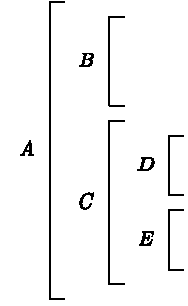
\includegraphics[width=.25\textwidth]{img/link-statici.pdf}
	\end{figure}
	
	\noindent
	In generale, se un \textbf{sottoprogramma è annidato al livello \emph{k}, allora la catena statica da quel sottoprogramma è lunga \emph{k}}.\newline
	
	\noindent
	Inoltre, è il \textbf{chiamate (Ch) a determinare il link statico del chiamato} usando le informazioni che ha a disposizione. Come per esempio l'annidamento statico dei blocchi e l'indirizzo del proprio Record di Attivazione. Il \textbf{processo eseguito dal chiamante viene effettuato determinando la catena statica del chiamante un numero di volte pari alla profondità di annidamento}, calcolata a tempo di compilazione, come \textbf{differenza} tra la \textbf{profondità statica del chiamante} e la \textbf{profondità statica del sottoprogramma} nel quale il chiamato viene definito.\newpage
	
	\subsubsection{Come determinare i link statici}
	
	Data una procedura \textbf{chiamante} Ch che chiama un'\textbf{altra procedura} P, Ch è in grado di determinare:
	\begin{itemize}
		\item Se $k = 0$, e di capire quindi che P è immediatamente inclusa nel chiamante Ch.\newline
		Nella pratica Ch passa a P il proprio puntatore (indirizzo) come link statico;
		
		\item Se $k > 0$, e di capire quindi che P è inclusa in un blocco che si trova $k$ passi fuori/prima di Ch.\newline
		Nella pratica, il chiamante Ch risale la propria catena statica di $k$ passi e passa il corrispondente puntatore (indirizzo) come link statico di P.
	\end{itemize}
	Il \textcolor{Red3}{\textbf{calcolo per ottenere}} $k$ da parte del chiamante:
	\begin{equation*}
		k = Sd\left(Ch\right) - Sd\left(P\right) + 1
	\end{equation*}
	\begin{itemize}
		\item $Sd\left(Ch\right)$ è la \textbf{profondità statica} (di annidamento) del \textbf{chiamante} \textbf{Ch};
		
		\item $Sd\left(P\right)$ è la \textbf{profondità statica} della \textbf{procedura} chiamata P.
	\end{itemize}
	Considerando come \textcolor{Green4}{\textbf{esempio}} la rappresentazione grafica presentata nella pagina precedente:
	\begin{enumerate}
		\item $A$ è la procedura \textsf{main} che chiama la procedura $B$. Al momento della chiamata da parte del chiamante $A$, Ch, cioè $A$, calcola:
		\begin{equation*}
			k = Sd\left(A\right) - Sd\left(B\right) + 1 = 0 - 1 + 1 = 0
		\end{equation*}
		Quindi, il link statico CS della procedura $B$ è pari a quello del chiamante $A$. Infatti, $A$ passa a $B$ il proprio indirizzo;
		
		\item La procedura chiamante $B$ chiama la procedura $C$ ed esegue il calcolo:
		\begin{equation*}
			k = Sd\left(B\right) - Sd\left(C\right) + 1 = 1 - 1 + 1 = 1
		\end{equation*}
		Quindi, significa che la procedura $B$ risale di $1$ la sua catena statica (raggiungendo la procedura $A$) e restituisce il link statico della procedura $C$ al Record di Attivazione raggiunto, cioè $A$;
		
		\item La procedura chiamante $C$ chiama la procedura $D$ ed esegue il calcolo:
		\begin{equation*}
			k = Sd\left(C\right) - Sd\left(D\right) + 1 = 1 - 2 + 1 = 0
		\end{equation*}
		Quindi, significa che la procedura chiamante $C$ passa il proprio indirizzo come link statico per raggiungere la procedura $D$;
		
		\item La procedura chiamante $D$ chiama la procedura $E$ ed esegue il calcolo:
		\begin{equation*}
			k = Sd\left(D\right) - Sd\left(E\right) + 1 = 2 - 2 + 1 = 1
		\end{equation*}
		Quindi, significa che la procedura $D$ risale di $1$ la propria catena statica, raggiungendo la procedura $C$, e restituisce il link statico della procedura $E$ al Record di Attivazione raggiunto, cioè $C$;
		
		\item La procedura chiamante $E$ chiama la procedura $C$ ed esegue il calcolo:
		\begin{equation*}
			k = Sd\left(E\right) - Sd\left(C\right) + 1 = 2 - 1 + 1 = 2
		\end{equation*}
		Quindi, significa che la procedura $E$ risale di $2$ la propria catena statica, seguendo prima il link che porta dalla procedura $E$ alla procedura $C$, e successivamente il link che porta dalla procedura $C$ alla procedura $A$. In questo modo, raggiunge la procedura $A$ e restituisce il link come statico della procedura $C$ al Record di Attivazione raggiunto, cioè $A$.
	\end{enumerate}
	E ancora, si porta qua di seguito un altro \textcolor{Green4}{\textbf{esempio}}, riportando prima il codice:\label{esempio risolvere riferimenti}
	\begin{lstlisting}[language=C]
void main() {
	int x;
	void A() {
		x = x + 1;
	}
	void B() {
		int x;
		void C(int y) {
			int x;
			x = y + 2;
			A();
		}
		x = 0;
		A();
		C(3);
	}
	x = 10;
	B();
}\end{lstlisting}
	Le relative profondità statiche iniziali e la rappresentazione grafica è la seguente:
	\begin{figure}[!htp]
		\centering
		\includegraphics[width=.8\textwidth]{img/link-statici-2.pdf}
	\end{figure}\newpage
	
	\noindent
	Le profondità statiche dopo le varie esecuzioni in ordine cronologico:
	\begin{enumerate}
		\item $B: Sd\left(\textsf{main}\right) - Sd\left(B\right) + 1 = 0$;\newline
		Il link statico di $B$ è l'indirizzo \textsf{main}: $CS\left(B\right) = \text{Indirizzo}\left(\textsf{main}\right)$;
		
		\item $A: Sd\left(B\right) - Sd\left(A\right) + 1 = 1$;\newline
		Il link statico di $A$ è l'indirizzo statico restituito da $B$: $CS\left(A\right) = \text{Indirizzo}\left(CS\left(B\right)\right)$;
		
		\item $C: Sd\left(B\right) - Sd\left(C\right) + 1 = 0$;\newline
		Il link statico di $C$ è l'indirizzo $B$: $CS\left(C\right) = \text{Indirizzo}\left(B\right)$;

		\item $A: Sd\left(C\right) - Sd\left(A\right) + 1 = 2$;\newline
		Il link statico di $A$ è l'indirizzo statico restituito da $C$ dell'indirizzo statico restituito da $B$: $CS\left(A\right) = \underbrace{\text{Indirizzo}\left(CS\left(CS\left(C\right)\right)\right)}_{\text{Risalita della catena statica}}$;
	\end{enumerate}
	Il Record di attivazione durante tutta l'esecuzione:
	\begin{figure}[!htp]
		\centering
		\includegraphics[width=.3\textwidth]{img/link-statici-3.pdf}
	\end{figure}\newpage

	\subsubsection{Risolvere i riferimenti}
	Nel paragrafo precedente è stata calcolata la catena statica, adesso viene spiegato come \textbf{risolvere i riferimenti}.\newline
	
	\noindent
	Dato che è noto dove viene definita ogni variabile, cioè è noto staticamente quali sono i sottoprogrammi che la definiscono, allora è \textbf{possibile determinare quale è il sottoprogramma più vicino} (nella catena di annidamento) che definisce la variabile. Per identificare tale programma, viene utilizzato un \textbf{valore} $N$ che \textbf{rappresenta il numero di volte necessario per risalire la catena statica}:
	\begin{equation*}
		N = Sd\left(P\right) - Sd\left(D\right)
	\end{equation*}
	\begin{itemize}
		\item $Sd\left(P\right)$ è la profondità statica del sottoprogramma $P$ in cui viene \textbf{utilizzato un identificatore};
		\item $Sd\left(D\right)$ è la profondità statica del sottoprogramma $D$ più vicino che \textbf{definisce un identificatore}.
	\end{itemize}
	Dato che per ogni identificatore utilizzato nel sottoprogramma $P$, l'antenato statico più vicino che definisce tale identificatore è $D$, allora il valore $N$ \textbf{indica quante volte è necessario risalire la catena statica per trovare esattamente il Record di Attivazione} di $D$.
	
	Al raggiungimento del Record di Attivazione, viene applicato (\textbf{sommato}) l'\emph{\textbf{offset}} così da trovare l'\textbf{esatta locazione da utilizzare}, cioè colei che contiene il valore dell'identificatore.\newline
	
	\noindent
	Questo metodo apporta un \textcolor{Green4}{\textbf{grande vantaggio}} poiché la ricerca dell'identificatore \underline{non} avviene più cercando in ogni antenato statico, ma trovando \underline{direttamente} l'antenato corretto contenente il giusto identificatore.\newpage
	
	\noindent
	Si prenda come \textcolor{Green4}{\textbf{esempio}} il programma nelle pagine precedenti (\pageref{esempio risolvere riferimenti}), in cui la sequenza di chiamate era: \textsf{main}, $B$, $A$, $C$, $A$.\newline
	\begin{minipage}{.4\textwidth}
		\begin{lstlisting}[language=C]
void main() {
	int x;
	void A() {
		x = x + 1;
	}
	void B() {
		int x;
		void C(int y) {
			int x;
			x = y + 2;
			A();
		}
		x = 0;
		A();
		C(3);
	}
	x = 10;
	B();
}\end{lstlisting}
	\end{minipage}
	\begin{minipage}{.6\textwidth}
		\begin{center}
			\includegraphics[width=.6\textwidth]{img/link-statici-3.pdf}
		\end{center}
	\end{minipage}
	
	\begin{enumerate}
		\item Nel \textsf{main} viene usata la variabile \textsf{x} che è locale e inizialmente inizializzata a 10;
		
		\item In $B$ viene usata una variabile \textsf{x}, anch'essa locale, che viene inizializzata a 0;
		
		\item $B$ esegue la chiamata alla procedura $A$, la quale usa una variabile \textsf{x} non locale. Quindi, è necessario eseguire il calcolo per capire di quanto risalire la catena statica per trovare l'identificatore \textsf{x}. L'antenato statico più vicino ad $A$ che definisce \textsf{x} è il \textsf{main} e infatti il calcolo eseguito è:
		\begin{equation*}
			N = Sd\left(A\right) - Sd\left(\textsf{main}\right) = 1 - 0 = 1
		\end{equation*}
		Quindi, nello stack, il link statico di $A$ punta esattamente al Record di Attivazione in cui è presente la \textsf{x} corretta.\newline
		Dopo questa verifica, $A$ esegue la sua procedura incrementando la \textsf{x} di 1 ($= 11$).
		
		\item In $C$ viene usata una variabile \textsf{x}, anch'essa locale, che viene inizializzata a 5;
		
		\item $C$ esegue la chiamata alla procedura $A$, la quale usa una variabile \textsf{x} non locale. Quindi, è necessario eseguire il calcolo per capire di quanto risalire la catena statica per trovare l'identificatore \textsf{x}. L'antenato statico più vicino ad $A$ che definisce \textsf{x} è il \textsf{main} e infatti il calcolo eseguito è:
		\begin{equation*}
			N = Sd\left(A\right) - Sd\left(\textsf{main}\right) = 1 - 0 = 1
		\end{equation*}
		Quindi, nello stack, il link statico di $A$ punta esattamente al Record di Attivazione in cui è presente la \textsf{x} corretta.\newline
		Dopo questa verifica, $A$ esegue la sua procedura incrementando la \textsf{x} di 1 ($= 12$).
	\end{enumerate}\newpage
	
	\subsection{Implementare lo scope dinamico}
	
	Nello \textbf{scope dinamico}, i riferimenti vanno risolti nell'ultimo blocco aperto e non ancora chiuso. Quindi, l'associazione nomi-oggetti denotabili dipende dal flusso del controllo a tempo di esecuzione, ovvero dall'ordine con cui i sottoprogrammi sono chiamati (definizione~\ref{scope statico e dinamico}).\newline
	
	\noindent
	La \textbf{regola generale} da seguire \textbf{per implementare lo scope dinamico} è la seguente: \textbf{l'associazione corrente per un nome è quella determinata per ultima nell'esecuzione e non ancora distrutta}.\newline
	
	\noindent
	L'\textbf{implementazione} può essere eseguita tramite due tecniche:
	\begin{itemize}
		\item \textcolor{Red3}{\textbf{Deep Access}} è l'implementazione più semplice e prevede che le \textbf{variabili non locali vengano trovate cercando nei Record di Attivazione lungo la catena dinamica}.\newline
		I \textbf{problemi} riscontrati sono molteplici e gravi:
		\begin{itemize}
			\item La lunghezza della catena non può essere determinata staticamente;
			\item Ogni Record di Attivazione deve avere i nomi delle variabili per poterli cercare risalendo la catena dinamica delle chiamate.
		\end{itemize}
		
		\item \textcolor{Red3}{\textbf{Shallow Access}} è la soluzione migliore in cui le \textbf{variabili locali vengono poste in strutture dati centrali}. Quindi, viene costruito uno stack per ogni nome di variabile e viene mantenuta una tabella centrale con una \emph{entry} per ogni nome di variabile.
	\end{itemize}\newpage
	
	\subsubsection{Implementazione Shallow Access: Tabella centrale dei riferimenti (CRT)}
	
	Una possibile \textbf{implementazione} della tecnica \emph{Shallow Access} è l'uso della \textcolor{Red3}{\textbf{tabella centrale dei riferimenti (CRT)}}. Essa è una \textbf{tabella} e ha le seguenti caratteristiche:
	\begin{itemize}
		\item Una \textbf{\emph{entry} per ogni variabile} presente nel programma;
		
		\item Le \textbf{\emph{entry} puntano ad una lista} di elementi;
		
		\item Le \textbf{liste di elementi} contengono le \textbf{informazioni necessarie per accedere ad un} possibile \textbf{ambiente} di riferimento.
	\end{itemize}
	L'\textbf{\underline{aggiornamento} della CRT} è il seguente. All'\textbf{aggiunta di un Record di Attivazione sullo stack}, \textbf{in cima} alla tabella viene \textbf{aggiunto un elemento} che fa \textbf{riferimento all'ambiente della procedura chiamata}. Il numero di elementi aggiunti dipende dal numero di identificatori definiti nella procedura chiamata.
		
	Quindi, per ogni identificatore del programma, l'ambiente di riferimento attivo è sempre quello in cima alla lista corrispondente all'identificatore nella tabella.\newline
	
	\noindent
	L'\textbf{\underline{utilizzo} della CRT} è il seguente. Viene \textbf{eseguito un accesso alla testa della sua lista} nella tabella e vengono \textbf{recuperate le informazioni necessarie per reperire nello stack l'ambiente di riferimento corretto}. Ad \textbf{ogni uscita da una procedura}, è importante \textbf{eliminare} anche dalla \textbf{tabella} gli \textbf{elementi in testa} che si riferiscono alla procedura terminata.\newline
	
	\noindent
	Per \textcolor{Green4}{\textbf{esempio}}, nel seguente schema, quando la procedura $D$ termina è necessario eliminare la testa della lista corrispondente a $w$.
	\begin{figure}[!htp]
		\centering
		\includegraphics[width=\textwidth]{img/CRT.pdf}
	\end{figure}\newpage
	
	\noindent
	I diversi \textcolor{Green4}{\textbf{vantaggi}} dell'implementazione della CRT:
	\begin{itemize}
		\item Vengono \textbf{evitate} le \textbf{lunghe scansioni di liste};
		
		\item La \textbf{tabella ha dimensione costante} se i nomi delle variabili sono noti staticamente;
		
		\item L'\textbf{accesso è in tempo costante} nonostante i costi di gestione in ingresso e uscita.
	\end{itemize}
	Un altro \textcolor{Green4}{\textbf{esempio}} è il seguente codice:
	\lstinputlisting[language=C]{code/esempio-CRT.c}\newpage
	
	\noindent
	Con il relativo grafico in cui è possibile verificare l'andamento:	
	\begin{figure}[!htp]
		\centering
		\includegraphics[width=\textwidth]{img/CRT-ex1.pdf}
	\end{figure}\newpage
	
	\subsection{Aggiunta delle procedure a $IMP$}
	
	Nel seguente paragrafo vengono aggiunte le procedure al linguaggio $IMP$.\newline
	
	\noindent
	Le \textbf{procedure} devono essere \textbf{dichiarate}, ovvero è necessario \textbf{definire l'associazione tra nome e astrazione nell'ambiente}. Quindi, deve essere modificata la categoria sintattica delle dichiarazioni:
	\begin{equation*}
		\begin{array}{rll}
			\mathrm{<Dec>} & & \\
			\mathrm{D} & \rightarrow & \mathrm{nil} \:\: | \:\: \textsf{const} \: \mathrm{I}:\tau = \mathrm{e} \:\: | \:\: \textsf{var} \: \mathrm{I} : \tau = \mathrm{e} \\
			&& \mathrm{D} \: \mathrm{in} \: \mathrm{D} \:\: | \:\: \mathrm{D} \: ; \: \mathrm{D} \:\: | \:\: \rho \\
			&& \textsf{proc} \: \mathrm{P()} \: \mathrm{C}
		\end{array}
	\end{equation*}
	Questa modifica rappresenta l'aggiunta della dichiarazione di procedura dove $P$ è il \textbf{nome della procedura}, mentre $C$ è il \textbf{corpo}, ovvero il codice da eseguire quando la procedura $P$ viene utilizzata.\newline
	
	\noindent
	Oltre alla dichiarazione, le \textbf{procedure} devono essere richiamate per essere \textbf{eseguite}. Il controllo deve passare alla procedura quando viene richiesto, quindi viene modificata la categoria sintattica dei comandi:
	\begin{equation*}
		\begin{array}{rll}
			\mathrm{<Com>} & & \\
			\mathrm{C} & \rightarrow & \mathrm{skip} \:\: | \:\: \mathrm{I} \coloneq \mathrm{e} \:\: | \:\: C \: ; \: C \:\: \\
			&& \textsf{if} \:\: \mathrm{B} \:\: \textsf{then} \:\: \mathrm{C} \:\: \textsf{else} \:\: \mathrm{C} \:\: | \\
			&& \textsf{while} \:\: \mathrm{B} \:\: \textsf{do} \:\: \mathrm{C} \:\: | \:\: \left\{\mathrm{D \: ; \: \mathrm{C}}\right\} \:\: | \:\: \mathrm{P()}
		\end{array}
	\end{equation*}
	Questa modifica rappresenta l'aggiunta di un comando per chiamare la procedura di nome $P$ durante l'esecuzione.\newpage
	
	\subsubsection{Semantica delle dichiarazioni}
	
	Per l'elaborazione di una dichiarazione, è necessario costruire l'ambiente statico corrispondente alla dichiarazione. Quindi, viene introdotto un \textbf{nuovo tipo} che consente di identificare gli identificatori che si riferiscono a procedure:
	\begin{equation*}
		\mathrm{DTyp} = \left\{\mathrm{int}, \mathrm{intloc}, \mathrm{bool}, \mathrm{boolloc}, \mathbf{proc}\right\}
	\end{equation*}
	Si definisce l'\textbf{ambiente statico} corrispondente ad una \textbf{dichiarazione di procedura} e si \textbf{stabilisce quando} una \textbf{tal dichiarazione è ben formata}:
	\begin{equation*}
		\mathcal{D}\mathrm{s}_{7} : \dfrac{
			\Delta \vdash_{\mathrm{V}} \: \mathrm{C}
		}{
			\Delta\vdash_{\mathrm{V}} \: \textsf{proc} \:\:\: \mathrm{P()} \: \mathrm{C}:\left[\mathrm{P} = \textsf{proc}\right]
		}
	\end{equation*}
	Quindi, se la procedura è ben formata, l'ambiente statico determinato dalla dichiarazione è quello che associa al nome P il tipo \textsf{proc}.\newline
	
	\noindent
	La \textbf{semantica dinamica} riguarda l'\textbf{elaborazione di una dichiarazione}, la quale ha l'obbiettivo, partendo da una determinata memoria iniziale, di \textbf{ottenere un ambiente dinamico determinato dalla dichiarazione stessa}.
	
	Tuttavia, la regola deve essere costruita tenendo in considerazione anche il tipo di scope:
	\begin{itemize}
		\item Scope \emph{statico}, è necessario \dquotes{\textbf{congelare}} e avere \textbf{sempre a disposizione l'ambiente valido al momento della definizione}, così da utilizzarlo quando la procedura viene chiamata.
		
		\item Scope \emph{dinamico}, la \textbf{procedura viene eseguita nell'ambiente valido al momento della chiamata}, quindi non è necessario il procedimento fatto per lo scope statico.
	\end{itemize}
	Quindi, la regola è la seguente:
	\begin{equation*}
		\mathcal{D}_{12} : \:\: \rho \: \vdash_{\mathrm{V}} \: \left\langle \textsf{proc} \:\: \mathrm{P()} \: \mathrm{C}, \sigma \right\rangle \longrightarrow_{\mathrm{d}} \left\langle \left[\mathrm{P} \leftarrow \lambda \varepsilon . \mathrm{C}'\right], \sigma \right\rangle
	\end{equation*}
	In cui $\mathrm{C}'$ è determinato dallo scope:
	\begin{itemize}
		\item Statico: $\mathrm{C}' = \rho_{|F|\left(C\right)} \: ; \: \mathrm{C}$
		
		\item Dinamico: $\mathrm{C}' = \mathrm{C}$
	\end{itemize}
	Quindi, nello scope statico viene preso l'ambiente valido al momento della definizione e viene fissato come ambiente in cui eseguire il corpo componendolo sequenzialmente con il corpo stesso.\newpage
	
	\subsubsection{Semantica dei comandi}
	
	L'\textbf{esecuzione di una chiamata} è un processo strutturato in più passaggi:
	\begin{enumerate}
		\item Stabilire quando una chiamata è ben formata (semantica statica);
		
		\item Passare il controllo dal chiamante al corpo della procedura (semantica dinamica).
	\end{enumerate}
	La \textbf{chiamata di una procedura è ben formata} quando \textbf{utilizza} un identificatore che ha \textbf{come tipo \textsf{proc}}, cioè il \dquotes{tipo procedura}:
	\begin{equation*}
		\mathcal{E}\mathrm{s}_{7}: \:\: \Delta\vdash_{\mathrm{V}} \: \mathrm{P()} \:\:\: \Delta\left(\mathrm{P}\right) = \textsf{proc}
	\end{equation*}
	Quindi, non esiste nessun vincolo statico, eccetto la restrizione del tipo del nome utilizzato.\newline
	
	\noindent
	Per la \textbf{semantica dinamica}, vi è il passaggio di controllo dal comando chiamante al corpo della procedura:
	\begin{equation*}
		\mathcal{E}_{14} : \:\: \rho \: \vdash_{\Delta} \: \left\langle \mathrm{P()}, \sigma \right\rangle \longrightarrow_{\mathrm{c}} \left\langle \mathrm{C}', \sigma \right\rangle \:\:\: \rho\left(\mathrm{P}\right) = \lambda\varepsilon . \mathrm{C}'
	\end{equation*}
	Per \textcolor{Green4}{\textbf{esempio}}, si definisce la seguente procedura:
	\begin{lstlisting}[language=C]
proc esempio() {	
	var x: int = 5;	
	z := x + y		
}\end{lstlisting}
	In cui tutta la procedura è rappresentata dalla lettera $d$, mentre il corpo dalla lettera $c$. La sua definizione è la seguente:
	\begin{gather*}
		\left[y \leftarrow 3\right] \: \vdash \left\langle d, \sigma \right\rangle \longrightarrow_{d} \left[\text{esempio} \leftarrow \lambda\varepsilon . \mathrm{C}'\right] \\
		\begin{array}{lll}
			\text{scope statico} 	&:&	\mathrm{C}' = \left[y \leftarrow 3\right] \: ; \: \mathrm{C} \\
			\text{scope dinamico} 	&:& \mathrm{C}' = \mathrm{C}
		\end{array}
	\end{gather*}
	Invece, la sua chiamata è la seguente:
	\begin{gather*}
		\left[y \leftarrow 4\right] \: \vdash \: \left\langle \text{esempio}(), \sigma \right\rangle \longrightarrow_{\mathrm{c}} \left\langle \mathrm{C}', \sigma \right\rangle \\
		\begin{array}{lll}
			\text{scope statico riferito a } \mathrm{C}' 	&:&	\left[y \leftarrow 4\right] \: \vdash \: \left\langle \left[y \leftarrow 3\right] \: ; \: \mathrm{C}, \sigma \right\rangle \longrightarrow_{\mathrm{C}} \cdots \\
			\text{scope dinamico riferito a } \mathrm{C}' 	&:& \left[y \leftarrow 4\right] \: \vdash \: \left\langle \mathrm{C}, \sigma \right\rangle \longrightarrow_\mathrm{C} \cdots
		\end{array}
	\end{gather*}\newpage
	
	\subsection{Parametrizzare le procedure}
	
	Oltre alle procedure, durante la loro definizione e chiamata, esistono altri valori, come i \textbf{parametri}, che hanno un'importanza significativa.\newline
	
	\noindent
	Durante la \textbf{definizione di una procedura}, i parametri vengono chiamati \textcolor{Red3}{\textbf{parametri formali}}. Un parametro formale è una \textbf{variabile listata nell'header} (interfaccia) e \textbf{utilizzata nel codice che definisce il sottoprogramma}. Un \textcolor{Green4}{\textbf{esempio}}:
	\begin{equation*}
		\textsf{int} \:\: \textsf{f} \:\: \left(\textsf{int} \:\: \textsf{n}\right) \hspace{1em} \left\{\textsf{return} \:\: \textsf{n}+1;\right\}
	\end{equation*}
	Dove la \textsf{n} è un parametro formale.\newline
	
	\noindent
	Durante la \textbf{chiamata di una procedura}, i parametri vengono chiamati \textcolor{Red3}{\textbf{parametri attuali}}. Un parametro attuale è un \textbf{valore} o un \textbf{indirizzo usato nel comando di chiamata per istanziare i parametri formali al valore da utilizzare quando il sottoprogramma viene eseguito}. Un \textcolor{Green4}{\textbf{esempio}}:
	\begin{equation*}
		\textsf{x} = \textsf{f}(\textsf{y} + 3);
	\end{equation*}
	Dove \textsf{y+3} è un parametro attuale.\newline
	
	\noindent
	Un altro aspetto da considerare è il \textbf{\emph{binding} effettuato tra parametri attuali e formali}. Questo può essere realizzato in due modi:
	\begin{itemize}
		\item \textcolor{Red3}{\textbf{Posizionale}}, il \emph{binding} tra \textbf{parametri attuali e formali è dato dalla posizione} (il primo parametro attuale è legato al primo formale e così via).\newline
		Questa metodologia è \textbf{sicura} ed \textbf{effettiva}.
		
		\item \textcolor{Red3}{\textbf{Keyword}}, il \textbf{nome del parametro formale} a cui un parametro attuale si riferisce, \textbf{è specificato insieme al parametro attuale al momento della chiamata}.\newline
		\textcolor{Green4}{\textbf{Vantaggio:}} i parametri possono apparire in qualunque ordine, evitando errori di corrispondenza.\newline
		\textcolor{Red4}{\textbf{Svantaggio:}} l'utente deve conoscere i nomi dei parametri formali.
	\end{itemize}
	Infine, è bene precisare che alcuni linguaggi ammettono \textbf{parametri attuali di default} nel caso in cui non vengano passati esplicitamente.\newpage
	
	\subsection{Passaggio dei parametri}
	
	Il \textbf{legame tra parametri attuali e parametri formali} avviene tramite modelli di comunicazione o modelli concettuali:
	\begin{itemize}
		\item \textcolor{Red3}{\textbf{Modelli di comunicazione}}, specifica quale direzione si sposta l'informazione tra chiamante e chiamato:
		\begin{itemize}
			\item \textcolor{Red3}{\textbf{\emph{In-mode}}}: $\textsf{main} \Rightarrow \textsf{proc}$.\newline
			L'\textbf{informazione viaggia in un'unica direzione dal chiamante al sottoprogramma}, il quale è chiamato mediante l'uso dei parametri. Anche l'ambiente non locale contribuisce al passaggio.
			
			\item \textcolor{Red3}{\textbf{\emph{Out-mode}}}: $\textsf{main} \Leftarrow \textsf{proc}$.\newline
			L'\textbf{informazione viagga in un'unica direzione dal chiamato al chiamante} sempre mediante l'uso dei parametri. Sia l'ambiente non locale che la possibilità di restituire un valore contribuiscono al passaggio.
			
			\item \textcolor{Red3}{\textbf{\emph{InOut-mode}}}: $\textsf{main} \iff \textsf{proc}$.\newline
			L'\textbf{informazione viaggia in entrambe le direzioni tra chiamante e chiamato}, sia mediante i parametri che mediante l'ambiente non locale e il valore di ritorno.
		\end{itemize}
		
		\item \textcolor{Red3}{\textcolor{Red3}{\textbf{Modelli concettuali}}}, specifica come il valore, fisicamente parlando, si sposta tra chiamante e chiamato:
		\begin{itemize}
			\item \textbf{Spostare fisicamente il valore mediante una copia del valore nel parametro formale};
			
			\item \textbf{Spostare un accesso al valore}.
		\end{itemize}
	\end{itemize}
	
	\begin{figure}[!htp]
		\centering
		\includegraphics[width=\textwidth]{img/passaggio_dei_parametri.png}
	\end{figure}\newpage
	
	\subsubsection{Passaggio per valore}\label{passaggio per valore}
	
	Il \textcolor{Red3}{\textbf{passaggio per valore}} \textbf{implementa un passaggio \emph{in-mode}} (dal chiamante al sottoprogramma) che richiede la valutazione completa del parametro prima del passaggio, come per \textcolor{Green4}{\textbf{esempio}} nel linguaggio C.\newline
	
	\noindent
	Quindi, durante la \textbf{chiamata di una procedura}, il \textbf{parametro attuale} può essere \textbf{esclusivamente un'espressione}, ovvero un \emph{r-value} (rappresentazione di un valore). Al contrario, durante la \textbf{definizione di una procedura}, il \textbf{parametro formale} deve essere un \textbf{riferimento}, ovvero un \emph{l-value}.\newline
	
	\noindent
	Alla \textbf{chiamata di una procedura}, l'\textbf{ambiente locale} della procedura viene \textbf{esteso} con l'associazione tra parametri attuali e parametri formali. Quest'ultimi vengono visti come variabili locali, ovvero vengono inizializzati con il valore dei parametri attuali.
	
	Il \textbf{passaggio di informazione è una semplice inizializzazione}, ovvero le \textbf{modifiche} dei \textbf{parametri formali} \underline{\textbf{non}} si \textbf{riflettono nei parametri attuali}. Quindi, non vi è un ritorno di informazione al chiamante mediante i parametri e questa è una \textcolor{Green4}{\textbf{caratteristica positiva}} che si adatta perfettamente alle funzioni matematiche, poiché \underline{non} genera \emph{side-effects}.\newline
	
	\noindent
	La \textbf{semantica} di questo metodo è la seguente: il \textbf{corpo non ha necessità di conoscere come la procedura verrà chiamata} (\textcolor{Red3}{\textbf{trasparenza referenziale}}), ma richiede \textbf{altri meccanismi} per permettere una comunicazione \emph{out-mode}.\newline
	
	\noindent
	L'\textbf{implementazione} avviene con la \textbf{creazione di una copia del valore} in quanto la trasmissione di un cammino richiederebbe una trasmissione protetta in scrittura.\newline
	
	\noindent
	Il passaggio per valore ha vantaggi e svantaggi:
	\begin{itemize}
		\item Il \textcolor{Green4}{\textbf{\underline{vantaggio}}} principale è la \textbf{velocità di passaggio per valori scalari};
		
		\item Lo \textcolor{Red3}{\textbf{\underline{svantaggio}}} principale è il \textbf{costo in spazio quando si passano valori di grandi dimensioni}.
	\end{itemize}
	Per \textcolor{Green4}{\textbf{esempio}}:
	\begin{lstlisting}[language=C]
void foo(int x) {
	x = x + 1;
}
...
y = 1;
foo(y + 1); // Qua y vale 1\end{lstlisting}
	Il parametro formale \textsf{x} è una variabile locale (sulla pila), alla chiamata, mentre il parametro attuale \textsf{y+1} è valutato e corrisponde al valore assegnato al parametro formale. Non viene creato nessun legame tra \textsf{x} nel corpo di \textsf{foo()} e \textsf{y} nel chiamante, ma solo una semplice copia del valore. Al ritorno dalla funzione \textsf{foo()}, il parametro formale \textsf{x} viene distrutto, ovvero tolto dalla pila.
	
	Questo procedimento implica che non è possibile trasmettere informazioni dalla funzione \textsf{foo()} al chiamante mediante il parametro.\newpage
	
	\noindent
	Un altro \textcolor{Green4}{\textbf{esempio}} è il seguente. Dato il seguente codice:
	\begin{lstlisting}[language=C]
void snap(value int a, value int b) {
	int tmp = a;
	a = b;
	b = tmp;
}
...
snap(c, d)\end{lstlisting}
	La situazione iniziale della memoria è la seguente:
	\begin{equation*}
		\sigma = \left[\textsf{c} \mapsto 3, \textsf{d} \mapsto 4\right]
	\end{equation*}
	Ovvero, la variabile \textsf{c} è uguale a $3$ e la variabile \textsf{d} è uguale a $4$. Le fasi del programma sono:
	\begin{enumerate}
		\item Alla \textbf{chiamata} della funzione \textsf{snap()}, il record di attivazione della funzione \textsf{snap()} diventa:
		\begin{equation*}
			\begin{array}{lll}
				\textsf{tmp}&\longrightarrow& \left[ \:\:\: \right] \\
				\textsf{a}	&\longrightarrow& \left[ 3 \right] \\
				\textsf{b}	&\longrightarrow& \left[ 4 \right]
			\end{array}
		\end{equation*}
		
		\item Al momento dell'\textbf{esecuzione} della funzione \textsf{snap()}, il record di attivazione diventa:
		\begin{equation*}
			\begin{array}{lll}
				\textsf{tmp}&\longrightarrow& \left[ 3 \right] \\
				\textsf{a}	&\longrightarrow& \left[ 4 \right] \\
				\textsf{b}	&\longrightarrow& \left[ 3 \right]
			\end{array}
		\end{equation*}
		
		\item Alla fine, ovvero nel momento in cui la funzione \textsf{foo()} \textbf{ritorna}, il record di attivazione viene eliminato e viene dunque liberato spazio in memoria.
	\end{enumerate}\newpage
	\begin{table}[!htbp]
		\centering
		\begin{tabular}{@{} l p{19em} @{}}
			\toprule
			Caratteristica & Descrizione \\
			\midrule
			\emph{In-mode} e valutazione parametri & Passaggio \emph{in-mode} (chiamante $\rightarrow$ sottoprogramma) e valutazione completa dei parametri. \\ [0.5em]
			Parametri attuali e formali & Il parametro attuale è un'espressione (\emph{r-value}) e il parametro formale è un riferimento (\emph{l-value}). \\ [0.5em]
			Inizializzazione semplice	& Il passaggio di informazione è una semplice inizializzazione, quindi le modifiche dei parametri formali non si riflettono nei parametri attuali. \\ [0.5em]
			Trasparenza referenziale	& Il corpo non ha necessità di conoscere come la procedura verrà chiamata. \\ [0.5em]
			Copia valore				& L'implementazione è una copia banale del valore. \\ [0.5em]
			Vantaggio: velocità			& Il vantaggio principale è la velocità di passaggio dei valori scalari. \\ [0.5em]
			Svantaggio: costo			& Lo svantaggio principale è il costo, in termini di spazio, dei valori di grandi dimensioni. \\
			\bottomrule
		\end{tabular}
		\caption{Caratteristiche del passaggio per valore.}
	\end{table}\newpage
	
	\subsubsection{Passaggio per risultato}\label{passaggio per risultato}
	
	Il \textcolor{Red3}{\textbf{passaggio per risultato}} prevede che \textbf{nessun valore venga trasmesso al sottoprogramma}. La \textbf{comunicazione tra chiamante e chiamato è di sola uscita} (\emph{\textbf{out-mode}}), ovvero prima di ritornare il controllo al chiamante, il \textbf{valore del parametro formale} (variabile locale) viene \textbf{copiato nel parametro attuale}. L'unica comunicazione possibile nella direzione opposta è usando l'ambiente globale.\newline
	
	\noindent
	Data la modalità \emph{out-mode}, il \textbf{parametro formale deve essere un valore}, ovvero un \emph{r-value}, mentre il \textbf{parametro attuale deve essere un riferimento}, cioè un \emph{l-value}.\newline
	
	\noindent
	Questa tecnica presenta \textcolor{Red3}{\textbf{vari problemi}} quali:
	\begin{itemize}
		\item \textbf{Collisione}. Il passaggio di due volte dello stesso parametro, il quale viene ricevuto in due parametri formali diversi.\newline
		Per \textcolor{Green4}{\textbf{esempio}}, la funzione \textsf{sub(p1, p1)} prende due parametri, ma in questo caso vengono passati due valori identici.
		
		\item \textbf{Ordine di valutazione dei parametri}. A seconda dell'ordine di valutazione dei parametri, la procedura può calcolare valori diversi.\newline
		Per \textcolor{Green4}{\textbf{esempio}}, la funzione definita:
		\begin{lstlisting}[language=C]
void fixer(out int x, out int y) {
	x = 17;
	y = 35;
}
...
fixer(out a, out a)\end{lstlisting}
		Se viene valutato prima \textsf{x} e poi \textsf{y} (nei parametri), allora il valore di \textsf{a} sarà 35, altrimenti sarà 17.
		
		\item L'implementazione sfrutta la copia del valore, quindi risulta \textbf{costoso} per dati di grandi dimensioni.
	\end{itemize}
	Per \textcolor{Green4}{\textbf{esempio}}, si consideri un'altra funzione:
	\begin{lstlisting}[language=C]
void foo(result int x) {
	x = 8;
}
...
y = 1;
foo(y); // Qui y vale 8\end{lstlisting}
	Il parametro formale è una variabile locale (sulla pila) e al ritorno dalla funzione \textsf{foo()}, il valore di \textsf{x} è assegnato al parametro attuale \textsf{y}. Non vi è nessun legame tra \textsf{x} nel corpo della funzione \textsf{foo()} e \textsf{y} nel chiamante. Al ritorno dalla funzione \textsf{foo()}, la \textsf{x} viene distrutta (rimossa dalla pila). Quindi, non vi è più possibile trasmettere informazioni dal chiamante alla funzione \textsf{foo()} mediante il parametro.\newpage
	
	\begin{table}[!htbp]
		\centering
		\begin{tabular}{@{} l p{18em} @{}}
			\toprule
			Caratteristica 	& Descrizione \\
			\midrule
			\emph{Out-mode} 			& Nessun valore viene trasmesso al sottoprogramma, la comunicazione tra chiamante e chiamato è di sola uscita. \\ [0.5em]
			Valore di ritorno			& Il valore del parametro formale (variabile locale) viene copiato nel parametro attuale e questo consente di ritornare un valore. \\ [0.5em]
			Valore - Riferimento		& Il parametro formale deve essere un valore (\emph{r-value}), mentre il parametro attuale deve essere un riferimento (\emph{l-value}). \\ [0.5em]
			Problema grave: collisione 	& Il passaggio di due volte dello stesso parametro, il quale viene ricevuto in due parametri formali diversi, crea alcune criticità. \\ [0.5em]
			Problema potenziale: ordine	& A seconda dell'ordine di valutazione dei parametri, la procedura può calcolare valori diversi. \\ [0.5em]
			Implementazione costosa		& L'implementazione sfrutta la copia del valore, quindi risulta costosa per dati di grandi dimensioni. \\
			\bottomrule
		\end{tabular}
		\caption{Caratteristiche del passaggio per risultato.}
	\end{table}\newpage
	
	\subsubsection{Passaggio per valore-risultato}
	
	Il \textcolor{Red3}{\textbf{passaggio per valore-risultato}} è un metodo \emph{InOut-mode}, ovvero consente una \textbf{comunicazione bidirezionale mediante i parametri}. Infatti, è un ibrido tra il passaggio per valore (paragrafo~\ref{passaggio per valore}) e il passaggio per risultato (paragrafo~\ref{passaggio per risultato}).\newline
	
	\noindent
	Nel caso di un passaggio per valore, il parametro attuale è anche un \emph{l-value}, ovvero una singola variabile. Quindi, \textsf{x+3} risulta inutilizzabile. Inoltre, \textbf{sia i parametri attuali che i parametri formali}, devono essere sia \emph{r-value} che \emph{l-value}, cioè \textbf{variabili}.\newline
	
	\noindent
	Un \textbf{potenziale effetto indesiderato} è il \emph{\textbf{side-effect}}. Esso si presenta solo al ritorno e indica che tutte le modifiche intermedie non sono visibili.\newline
	
	\noindent
	Il \textbf{valore del parametro attuale} viene utilizzato \textbf{solamente} per \textbf{inizializzare il parametro formale}, il quale successivamente agisce da variabile locale (\emph{local storage}). Al \textbf{termine dell'esecuzione del sottoprogramma}, il valore del \textbf{parametro formale è trasmesso all'attuale}.\newline
	
	\noindent
	Gli \textcolor{Red3}{\textbf{svantaggi}} e i \textcolor{Red3}{\textbf{potenziali problemi}} sono gli stessi dei due passaggi per valore e risultato. Rimane anche il problema delle copie di grandi dimensioni.\newline
	
	\noindent
	Nel seguente \textcolor{Green4}{\textbf{esempio}}, il parametro formale \textsf{x} è una variabile locale (sulla pila). Alla chiamata, il valore del parametro attuale è assegnato al parametro formale. Analogamente, al ritorno, il valore del parametro formale è assegnato al parametro attuale. Di conseguenza, non viene fissato nessun legame tra \textsf{x} nel corpo della funzione \textsf{foo()} e \textsf{y} nel chiamante. Al ritorno da \textsf{foo()}, la \textsf{x} viene distrutta, cioè rimossa dalla pila.
	\begin{lstlisting}[language=C]
void foo(value-result int x) {
	x = x + 1;
}
...
y = 8;
foo(y); // Qui y vale 9
	\end{lstlisting}\newpage
	
	\noindent
	Si propone qua di seguito un altro \textcolor{Green4}{\textbf{esempio}} con il seguente codice:
	\begin{lstlisting}[language=C]
void swap(value int a, values int b) {
	int tmp = a;
	a = b;
	b = tmp;
}
...
swap(c, d)\end{lstlisting}
	La situazione iniziale è la seguente:
	\begin{equation*}
		\sigma = \left[\textsf{c} \mapsto 3, \textsf{d} \mapsto 4\right]
	\end{equation*}
	Le fasi del programma sono:
	\begin{enumerate}
		\item La \textbf{chiamata} della funzione \textsf{swap} provoca il seguente cambio di memoria (copia valore):
		\begin{equation*}
			\begin{array}{lll}
				\textsf{tmp} &\longrightarrow& \left[ \:\:\: \right] \\
				\textsf{a} 	 &\longrightarrow& \left[ 3 \right] \\
				\textsf{b} 	 &\longrightarrow& \left[ 4 \right]
			\end{array}
		\end{equation*}

		\item All'\textbf{esecuzione} della funzione \textsf{swap}, i valori mutano nel seguente modo:
		\begin{equation*}
			\begin{array}{lll}
				\textsf{tmp} &\longrightarrow& \left[ 3 \right] \\
				\textsf{a} 	 &\longrightarrow& \left[ 4 \right] \\
				\textsf{b} 	 &\longrightarrow& \left[ 3 \right]
			\end{array}
		\end{equation*}

		\item Al \textbf{ritorno} dalla funzione \textsf{swap}, i valori nel \textsf{main} sono mutati e dunque diventano:
		\begin{equation*}
			\begin{array}{lll}
				\textsf{tmp} &\longrightarrow& \left[ 3 \right] \\
				\textsf{a} 	 &\longrightarrow& \cancel{\left[ 3 \right]} \dashrightarrow \left[4\right] \\
				\textsf{b} 	 &\longrightarrow& \cancel{\left[ 4 \right]} \dashrightarrow \left[3\right]
			\end{array}
		\end{equation*}
	\end{enumerate}
	\begin{table}[!htp]
		\centering
		\begin{tabular}{@{} l p{20em} @{}}
			\toprule
			Caratteristica & Descrizione \\
			\midrule
			\emph{InOut-mode}			& Comunicazione bidirezionale tramite l'uso di parametri. \\ [0.5em]
			Parametri sono variabili	& Sia i parametri attuali che i parametri formali devono essere variabili, ovvero \emph{r-value} e \emph{l-value}. \\ [0.5em]
			\emph{Side-effect}			& Effetto che si presenta solo al ritorno poiché tutte le modifiche intermedie non sono visibili. \\ [0.5em]
			Scopo del parametro attuale	& Il valore del parametro attuale è usato per inizializzare il parametro formale, poiché quest'ultimo viene usato come variabile locale. \\ [0.5em]
			Valore di ritorno			& Al termine dell'esecuzione del sottoprogramma, il valore del parametro formale viene trasmesso al parametro attuale. \\
			\bottomrule
		\end{tabular}
		\caption{Caratteristiche del passaggio per valore-risultato.}
	\end{table}\newpage
	
	\subsubsection{Passaggio per riferimento}
	
	Nel \textcolor{Red3}{\textbf{passaggio per riferimento}} viene \textbf{passato un cammino di accesso al parametro attuale}. Grazie a questa caratteristica, questo metodo prende anche il nome di \textcolor{Red3}{\textbf{passaggio per condivisione}} e la metodologia di comunicazione utilizzata è la \textbf{\emph{InOut-mode}} tramite i parametri.\newline
	
	\noindent
	In questo caso, i \textbf{parametri attuali devono essere riferimenti} (\emph{l-value}) e i \textbf{parametri formali prendono il riferimento} dato dagli attuali. Durante l'esecuzione, \textbf{tutti i riferimenti al valore} (\emph{r-value}) \textbf{del parametro formale}, sono \textbf{riferimenti al valore} (\emph{r-value}) \textbf{del parametro attuale}. Quindi, tutti i cambiamento effettuati dal parametro formale, avvengono anche nel parametro attuale.\newline
	
	\noindent
	Il \textbf{parametro formale è un indirizzo del parametro attuale} e quindi ogni utilizzo viene effettuato accedendo all'indirizzo presente nell'ambiente del chiamante. È chiaro dunque che le \textbf{modifiche avvengono dentro la locazione del parametro attuale}.\newline
	
	\noindent
	L'\textbf{implementazione} è \textbf{efficiente} poiché non esegue copie, \textbf{tuttavia può creare \emph{alias}}. Quindi, il \textcolor{Green4}{\textbf{principale vantaggio}} è l'efficienza del processo di passaggio poiché non avviene nessuna copia o duplicazione di \emph{storage}.\newline
	
	\noindent
	Al contrario, gli \textcolor{Red3}{\textbf{svantaggi}} possono essere molteplici:
	\begin{itemize}
		\item Accesso più lento ai parametri formali (rispetto agli metodi di comunicazione, come il passaggio per valore);
		
		\item Potenziali effetti collaterali (collisioni);
		
		\item Creazione di alias.
	\end{itemize}
	Per \textcolor{Green4}{\textbf{esempio}}, nel seguente codice viene definita una funzione.
	\begin{lstlisting}[language=C]
void foo(reference int x) {
	x = x + 1;
}
...
y = 1;
foo(y); // Qui y vale 2\end{lstlisting}
	Alla funzione viene passato un riferimento (indirizzo/puntatore) al parametro attuale, per questo motivo l'attuale deve essere un riferimento (\emph{l-value}). Il parametro formale \textsf{x} diventa quindi un alias di \textsf{y}. Al ritorno dalla funzione \textsf{foo()}, viene distrutto il legame tra \textsf{x} e l'indirizzo di \textsf{y}. Quindi, la trasmissione è bidirezionale tra chiamante e chiamato.\newpage
	
	\noindent
	Si propone qua di seguito un esempio con il seguente codice:
	\begin{lstlisting}[language=C]
void swap(ref int a, ref int b) {
	int tmp = a;
	a = b;
	b = tmp;
}
...
swap(c, d)\end{lstlisting}
	In cui la situazione iniziale della memoria è la seguente:
	\begin{equation*}
		\sigma = \left[\textsf{c} \mapsto 3, \textsf{d} \mapsto 4\right]
	\end{equation*}
	Le fasi del programma sono:
	\begin{enumerate}
		\item La \textbf{chiamata} della funzione \textsf{swap()} crea una serie di puntatori:
		\begin{equation*}
			\begin{array}{lllll}
				\textsf{tmp} &\longrightarrow& \left[ \:\:\: \right] \\
				\textsf{a} 	 &\longrightarrow& \left[ ^{*}\textsf{c} \right] &\longrightarrow^{*}& \textsf{c} = \left[3\right] \\
				\textsf{b} 	 &\longrightarrow& \left[ ^{*}\textsf{d} \right] &\longrightarrow^{*}& \textsf{d} = \left[4\right]
			\end{array}
		\end{equation*}

		\item L'\textbf{esecuzione} della funzione \textsf{swap()} cambia i valori che si trovano nelle locazioni a cui puntano \textsf{a} e \textsf{b}:
		\begin{equation*}
			\begin{array}{lllll}
				\textsf{tmp} &\longrightarrow& \left[ 3 \right] \\
				\textsf{a} 	 &\longrightarrow& \left[ ^{*}\textsf{c} \right] &\longrightarrow^{*}& \textsf{c} = \cancel{\left[3\right]} \dashrightarrow \left[4\right] \\
				\textsf{b} 	 &\longrightarrow& \left[ ^{*}\textsf{d} \right] &\longrightarrow^{*}& \textsf{d} = \cancel{\left[4\right]} \dashrightarrow \left[3\right]
			\end{array}
		\end{equation*}

		\item Al \textbf{ritorno} dalla funzione \textsf{swap()}, il record di attivazione viene rimosso dallo stack e quindi i puntatori vengono rimossi. Tuttavia, i parametri attuali hanno mutato il loro valore:
		\begin{equation*}
			\begin{array}{lllll}
				\cancel{\textsf{tmp}} &\cancel{\longrightarrow}& \cancel{\left[ 3 \right]} \\
				\cancel{\textsf{a}} 	 &\cancel{\longrightarrow}& \left[ ^{*}\textsf{c} \right] &\longrightarrow^{*}& \textsf{c} = \left[4\right] \\
				\cancel{\textsf{b}} 	 &\cancel{\longrightarrow}& \left[ ^{*}\textsf{d} \right] &\longrightarrow^{*}& \textsf{d} = \left[3\right]
			\end{array}
		\end{equation*}
	\end{enumerate}\newpage
	
	\noindent
	Un altro \textcolor{Green4}{\textbf{esempio}} un po' più complesso è il seguente:
	\begin{lstlisting}[language=C]
void fie(ref int x, ref int y) {
	y = 2;
	x = 5;
	if (x == y) then y = y + 2;
}
...
int a = 3;
fie(a, a);\end{lstlisting}
	Le fasi del programma sono:
	\begin{enumerate}
		\item Alla chiamata della funzione \textsf{fie()}, vengono passati due parametri attuali che si riferiscono alla stessa locazione di memoria:
		\begin{equation*}
			\begin{array}{lllll}
				\textsf{x} &\longrightarrow& \left[^{*} \textsf{a}\right] &\longrightarrow^{*}& \textsf{a} = \left[3\right] \\
				\textsf{y} &\longrightarrow& \left[^{*} \textsf{a}\right] &\longrightarrow^{*}& \textsf{a} = \left[3\right]
			\end{array}
		\end{equation*}
		
		\item All'esecuzione della funzione \textsf{fie()}, vengono eseguite una serie di operazioni:
		\begin{enumerate}
			\item Viene eseguito il comando \textsf{y = 2}:
			\begin{equation*}
				\begin{array}{lllll}
					\textsf{x} &\longrightarrow& \left[^{*} \textsf{a}\right] &\longrightarrow^{*}& \textsf{a} = \cancel{\left[3\right]} \dashrightarrow \left[2\right] \\
					\textsf{y} &\longrightarrow& \left[^{*} \textsf{a}\right] &\longrightarrow^{*}& \textsf{a} = \cancel{\left[3\right]} \dashrightarrow \left[2\right]
				\end{array}
			\end{equation*}
			
			\item Viene eseguito il comando \textsf{x = 5}:
			\begin{equation*}
				\begin{array}{lllll}
					\textsf{x} &\longrightarrow& \left[^{*} \textsf{a}\right] &\longrightarrow^{*}& \textsf{a} = \cancel{\left[2\right]} \dashrightarrow \left[5\right] \\
					\textsf{y} &\longrightarrow& \left[^{*} \textsf{a}\right] &\longrightarrow^{*}& \textsf{a} = \cancel{\left[2\right]} \dashrightarrow \left[5\right]
				\end{array}
			\end{equation*}
			
			\item Viene eseguito il comando \textsf{if (x == y) then y = y+2}:
			\begin{equation*}
				\begin{array}{lllll}
					\textsf{x} &\longrightarrow& \left[^{*} \textsf{a}\right] &\longrightarrow^{*}& \textsf{a} = \cancel{\left[5\right]} \dashrightarrow \left[7\right] \\
					\textsf{y} &\longrightarrow& \left[^{*} \textsf{a}\right] &\longrightarrow^{*}& \textsf{a} = \cancel{\left[5\right]} \dashrightarrow \left[7\right]
				\end{array}
			\end{equation*}
		\end{enumerate}
		Come si può osservare dalla mutazione della memoria, qualsiasi operazione che interessa uno dei due parametri formali, si riflette anche sull'altro.
		
		\item Al ritorno dalla funzione \textsf{fie()}, i puntatori vengono rimossi e la variabile \textsf{a} ha il valore aggiornato dopo le modifiche:
		\begin{equation*}
			\begin{array}{lllll}
				\cancel{\textsf{x}} &\cancel{\longrightarrow}& \cancel{\left[^{*} \textsf{a}\right]} &\cancel{\longrightarrow^{*}}& \textsf{a} = \left[7\right] \\
				\cancel{\textsf{y}} &\cancel{\longrightarrow}& \cancel{\left[^{*} \textsf{a}\right]} &\cancel{\longrightarrow^{*}}& \textsf{a} = \left[7\right]
			\end{array}
		\end{equation*}
	\end{enumerate}\newpage
	
	\begin{table}[!htp]
		\centering
		\begin{tabular}{@{} l p{19em} @{}}
			\toprule
			Caratteristica & Descrizione \\
			\midrule
			Passaggio per condivisione	& Al parametro attuale viene passato un cammino di accesso. \\ [0.5em]
			Parametri come riferimenti	& I parametri attuali devono essere riferimenti e i parametri formali prendono il riferimento dato dagli attuali. \\ [0.5em]
			Riferimenti bidirezionali	& Tutti i riferimenti al valore del parametro formale, sono riferimenti al valore del parametro attuale. \\ [0.5em]
			Indirizzo come parametro	& Il parametro formale è un indirizzo del parametro attuale e le modifiche avvengono dentro la locazione del parametro attuale. \\ [0.5em]
			Implementazione efficiente	& L'implementazione è efficiente poiché non esegue copie, tuttavia rimane la possibilità di eventuali alias. \\
			\bottomrule
		\end{tabular}
		\caption{Caratteristiche del passaggio per riferimento.}
	\end{table}\newpage
	
	\subsection{Aggiunta delle procedure con parametri a $IMP$}
	
	In questi paragrafi si \textbf{modificano le dichiarazioni} per consentire di dichiarare le \textbf{procedure che ricevono parametri}.\newline
	
	\noindent
	La \textbf{dichiarazione di procedura con parametri}, dove $P$ è il nome della procedura, $C$ è il corpo e \textsf{form} è la lista di parametri, è la seguente:
	\begin{equation*}
		\begin{array}{rll}
			\mathrm{<Dec>} & & \\
			\mathrm{D} & \rightarrow & \mathrm{nil} \:\: | \:\: \textsf{const} \: \mathrm{I}:\tau = \mathrm{e} \:\: | \:\: \textsf{var} \: \mathrm{I} : \tau = \mathrm{e} \\
			&& \mathrm{D} \: \mathrm{in} \: \mathrm{D} \:\: | \:\: \mathrm{D} \: ; \: \mathrm{D} \:\: | \:\: \rho \\
			&& \textsf{proc} \: \mathrm{P(\textsf{form})} \: \mathrm{C}
		\end{array}
	\end{equation*}
	Inoltre, viene \textbf{definita cosa è una lista di parametri}, ovvero una \textbf{lista di dichiarazioni di identificatori, variabili o costanti, senza inizializzazione}:
	\begin{equation*}
		form \Coloneq \bullet \:\: | \:\: \textsf{const} \:\: x : \tau, form \:\: | \:\: \textsf{var} \:\: x : \tau,form
	\end{equation*}
	In cui $\bullet$ rappresenta una lista vuota.\newline
	
	\noindent
	Alle dichiarazioni è necessario aggiungere anche una \textbf{forma di dichiarazione intermedia} che consenta di \textbf{creare}, nell'ambiente locale della procedura, le \textbf{associazioni tra i parametri formali e i parametri attuali}, descritti dalla lista \emph{ae}:
	\begin{gather*}
		ae \Coloneq \bullet \:\: | \:\: e, ae \\
		\begin{array}{rll}
			\mathrm{<Dec>} & & \\
			\mathrm{D} & \rightarrow & \mathrm{nil} \:\: | \:\: \textsf{const} \: \mathrm{I}:\tau = \mathrm{e} \:\: | \:\: \textsf{var} \: \mathrm{I} : \tau = \mathrm{e} \\
			&& \mathrm{D} \: \mathrm{in} \: \mathrm{D} \:\: | \:\: \mathrm{D} \: ; \: \mathrm{D} \:\: | \:\: \rho \\
			&& \textsf{proc} \: \mathrm{P(\textsf{form})} \: \mathrm{C} \hspace{1em} \textsf{form} = \textsf{ae}
		\end{array}
	\end{gather*}
	Dato che le procedure devono essere \textbf{chiamate}, per farlo serve utilizzare una lista di parametri attuali:
	\begin{equation*}
		\begin{array}{rll}
			\mathrm{<Com>} & & \\
			\mathrm{C} & \rightarrow & \mathrm{skip} \:\: | \:\: \mathrm{I} \coloneq \mathrm{e} \:\: | \:\: C \: ; \: C \:\: \\
			&& \textsf{if} \:\: \mathrm{B} \:\: \textsf{then} \:\: \mathrm{C} \:\: \textsf{else} \:\: \mathrm{C} \:\: | \\
			&& \textsf{while} \:\: \mathrm{B} \:\: \textsf{do} \:\: \mathrm{C} \:\: | \:\: \left\{\mathrm{D \: ; \: \mathrm{C}}\right\} \:\: | \:\: \mathrm{P(\textsf{ae})}
		\end{array}
	\end{equation*}\newpage
	
	\subsubsection{Semantica statica delle dichiarazioni}
	
	Si definiscono gli \textbf{identificatori liberi} e gli \textbf{identificatori definiti} delle nuove dichiarazioni:
	\begin{equation*}
		\begin{array}{lll}
			FI\left(\textsf{proc} \:\: P\left(form\right) C\right) &=& FI\left(C\right) \setminus DI\left(form\right) \\
			FI\left(form = ae\right) &=& FI\left(ae\right) \\
			FI\left(e, ae\right) &=& FI\left(e\right) \cup FI\left(ae\right) \\
			FI\left(\bullet\right) &=& \emptyset \\
			&& \\
			DI\left(\textsf{proc} \:\: P\left(form\right) C\right) &=& \left\{P\right\} \cup DI\left(form\right) \cup DI\left(C\right) \\
			DI\left(form = ae\right) &=& DI\left(form\right) \\
			DI\left(\textsf{const} \:\: x:\tau, form\right) &=& \left\{x\right\} \cup DI\left(form\right) \\
			DI\left(\textsf{var} \:\: x:\tau, form\right) &=& \left\{x\right\} \cup DI\left(form\right) \\
			DI\left(\bullet\right) &=& \emptyset
		\end{array}
	\end{equation*}
	La \textbf{semantica statica} corrisponde all'\textbf{ambiente statico creato dalle nuove dichiarazioni}. In particolare, l'ambiente statico viene creato dall'associazione tra parametri formali e parametri attuali. Quindi, si associa una lista di tipi formali:
	\begin{equation*}
		\begin{cases}
			\mathcal{T}\left(\bullet\right) = \bullet \\
			\\
			\mathcal{T}\left(\textsf{const} \:\: x:\tau, form\right) = \tau, \mathcal{T}\left(form\right) \\
			\\
			\mathcal{T}\left(\textsf{var} \:\: x,\tau, form\right) = \tau loc, \mathcal{T}\left(form\right)
		\end{cases}
	\end{equation*}
	Inoltre, viene \textbf{elaborata la lista di tipi di una lista di parametri attuali}:
	\begin{equation*}
		\begin{cases}
			\Delta\vdash_{I} \bullet : \bullet \\
			\\
			\dfrac{\Delta \: \vdash_{I} \: e : \tau, \: \Delta \: \vdash_{I} \: ae : aet}{\Delta \: \vdash_{I} \: e, \: ae : \tau, \: aet}
		\end{cases} \hspace{1em} aet \Coloneq \bullet \:\: | \:\: \tau, aet
	\end{equation*}
	Infine, viene \textbf{associato un ambiente statico ad una lista di parametri formali}:
	\begin{equation*}
		\begin{cases}
			\bullet : \emptyset \\
			\\
			\dfrac{form \: : \: \Delta_{0}}{\textsf{const} \:\: x:\tau, \: form : \Delta_{0} \left[x = \tau\right]}, & \Delta_{0} : I_{0}, \: x \notin I_{0} \\
			\\
			\dfrac{form \: : \: \Delta_{0}}{\textsf{var} \:\: x:\tau, \: form : \Delta_{0} \left[x = \tau loc\right]}, & \Delta_{0} : I_{0}, \: x \notin I_{0}
		\end{cases}
	\end{equation*}\newpage
	
	\noindent
	Per \textbf{elaborare una dichiarazione} è necessario costruire l'ambiente statico corrispondente. Quindi, deve essere modificata la regola per la dichiarazione di una procedura, la quale ha in generale una lista di parametri $\Delta_{0} : V'$:
	\begin{equation*}
		\mathcal{D}s_{7} : \dfrac{
			\textsf{form}:\Delta_{0} \hspace{1em} \Delta\left[\Delta_{0}\right] \vdash_{\mathrm{V} \cup \mathrm{V}'} \: \mathrm{C}
		}{
			\Delta \vdash_{\mathrm{V}} \: \textsf{proc} \:\: \textsf{P}\left(\textsf{form}\right) \textsf{C} : \left[\textsf{P} = \mathsf{F} \left(\textsf{form}\right) \textsf{proc}\right]
		}
	\end{equation*}
	L'\textbf{ambiente associato ai parametri formali} è costruito nel seguente modo. Si verifica che il corpo $C$ sia ben formato e a questo punto il tipo che viene associato alla procedura consiste nella lista dei tipi dei parametri formali seguiti dal suffisso \textsf{proc}, il quale evidenzia che l'identificatore è una procedura. Quindi, la \textbf{nuova regola per l'associazione tra parametri formali e parametri attuali}:
	\begin{equation*}
		\mathcal{D}\mathrm{s}_{8} : \dfrac{
			\textsf{form} : \Delta_{0} \hspace{1em} \Delta\vdash_{\mathrm{V}} \: \textsf{ae} : \mathcal{F}\left(\textsf{form}\right)
		}{
			\Delta\vdash_{\mathrm{V}} \: \textsf{form} = \textsf{ae} : \Delta_{0}
		}
	\end{equation*}
	Se la lista di tipi dei parametri attuali coincide con la lista dei tipi dei parametri formali ($\textsf{ae}:\mathcal{F}\left(\textsf{form}\right)$), allora l'ambiente statico generato dai parametri formali viene associato alla dichiarazione.\newpage
	
	\subsubsection{Semantica delle dichiarazioni}
	
	Per \textbf{elaborare le dichiarazioni} è necessario \textbf{aggiornare il sistema di regole considerando anche i parametri}. Quindi, nel valore associato al nome della procedura, si inseriscono anche i parametri formali. Ovviamente rimane inalterata la costruzione di $\textsf{C}'$ il quale dipende dal tipo di scope (statico/dinamico):
	\begin{equation*}
		\mathcal{D}_{13} : \:\: \rho \vdash_{\Delta} \: \left\langle \textsf{proc} \:\: \textsf{P}\left(\textsf{form}\right)\textsf{C}, \sigma \right\rangle \longrightarrow_{\mathrm{d}} \left\langle \left[P \leftarrow \lambda \textsf{form}.\textsf{C}'\right], \sigma \right\rangle
	\end{equation*}
	Si ricorda che:
	\begin{itemize}
		\item $\mathrm{C}' = \rho_{|F|\left(C\right)} ; \mathrm{C}$ per scoping statico;
		\item $\mathrm{C}' = \mathrm{C}$ per scoping dinamico.
	\end{itemize}
	Infine, è necessario \textbf{aggiungere la regola} per l'\textbf{associazione tra parametri attuali e parametri formali}, la quale richiede tutta una serie di nuove regole per la valutazione della lista dei parametri attuali:
	\begin{itemize}
		\item La regola $14$:
		\begin{equation*}
			\mathcal{D}_{14}: \dfrac{
				\rho \: \vdash_{\Delta} \: \left\langle \mathrm{e}, \sigma \right\rangle \longrightarrow_{\mathrm{e}} \left\langle \mathrm{e}', \sigma \right\rangle
			}{
				\rho \: \vdash_{\Delta} \: \left\langle \left(\mathrm{e}, \mathrm{ae}\right), \sigma \right\rangle \longrightarrow_{\mathrm{ae}} \left\langle \left(\mathrm{e}', \mathrm{ae}\right), \sigma \right\rangle
			}
		\end{equation*}
		
		\item La regola $15$:
		\begin{equation*}
			\mathcal{D}_{15}: \dfrac{
				\rho \: \vdash_{\Delta} \: \left\langle \mathrm{ae}, \sigma \right\rangle \longrightarrow_{\mathrm{ae}} \left\langle \mathrm{ae}', \sigma \right\rangle
			}{
				\rho \: \vdash_{\Delta} \: \left\langle \left(\mathrm{k}, \mathrm{ae}\right), \sigma \right\rangle \longrightarrow_{\mathrm{ae}} \left\langle \left(\mathrm{k}, \mathrm{ae}'\right), \sigma \right\rangle
			}
		\end{equation*}
		
		\item La regola $16$:
		\begin{equation*}
			\mathcal{D}_{16}: \dfrac{
				\rho \: \vdash_{\Delta} \: \left\langle \mathrm{ae}, \sigma \right\rangle \longrightarrow_{\mathrm{ae}} \left\langle \mathrm{ae}', \sigma \right\rangle
			}{
				\rho \: \vdash_{\Delta} \: \left\langle \textsf{form} = \textsf{ae}, \sigma \right\rangle \longrightarrow_{\mathrm{d}} \left\langle \textsf{form} = \mathrm{ae}', \sigma \right\rangle
			}
		\end{equation*}
	\end{itemize}
	Infine, per \textbf{utilizzare la lista di parametri attuali}, è necessario \textbf{creare l'ambiente dinamico e la memoria}, ovvero le associazioni corrispondenti:
	\begin{equation*}
		\mathcal{D}_{17} : \dfrac{
			\mathrm{ak}, \mathrm{L} \:\: \vdash \:\: \textsf{form}: \rho_{0}, \sigma_{0}
		}{
			\rho \: \vdash_{\Delta} \: \left\langle \textsf{form} = \mathrm{ak}, \sigma \right\rangle \longrightarrow_{\mathrm{d}} \left\langle \rho_{0}, \sigma\left[\sigma_{0}\right] \right\rangle
		}
	\end{equation*}
	La lista di parametri attuali $\mathrm{ak}$, insieme alla lista di parametri formali $\textsf{form}$, crea l'ambiente dinamico $\rho_{0}$ e la memoria $\sigma_{0}$. La dichiarazione $\textsf{form} = \mathrm{ae}$ viene elaborata nell'ambiente $\rho_{0}$ e con la memoria iniziale aggiornata da $\sigma_{0}$.\newline
	
	\noindent
	Per derivare la premessa, ovvero per \textbf{costruire l'ambiente e la memoria a partire da una lista di parametri attuali valutati e da una lista corrispondente di parametri formali}, è necessaria una definizione:
	\begin{gather*}
		\begin{cases}
			\bullet, \mathrm{L} \: \vdash \: \bullet \: \emptyset, \emptyset \\
			\\
			\dfrac{
				ak, \: L \vdash form: \rho_{0}, \sigma_{0}
			}{
				\left(k, ak\right), \: L \vdash \textsf{const} \: x:\tau, \: form \: : \rho_{0}\left[x = k\right], \: \sigma_{0}
			}, & k : \tau \\
			\\
			\dfrac{
				ak, \: L \cup \left\{l\right\} \vdash form: \rho_{0}, \sigma_{0}
			}{
				\left(k, ak\right), \: L \vdash \textsf{var} \: x:\tau, \: form \: : \rho_{0}\left[x = l\right], \: \sigma_{0}\left[l = k\right]
			}, & k : \tau, \hspace{1em} l \in New_{\tau}\left(L_{0}\right), \sigma_{0}:L_{0}
		\end{cases} \\
		\\
		ak \Coloneq \bullet \:\: | \:\: k, ak
	\end{gather*}\newpage
	
	\subsubsection{Semantica dei comandi}
	
	La \textbf{semantica dei comandi}, sia statica che dinamica, viene presentata nel seguente paragrafo.\newline
	
	\noindent
	Si definiscono gli \textbf{identificatori liberi e definiti}:
	\begin{equation*}
		\begin{array}{lll}
			DI\left(P\left(ae\right)\right) &=& \emptyset \\
			FI\left(P\left(ae\right)\right) &=& FI\left(ac\right) \cup \left\{P\right\}
		\end{array}
	\end{equation*}
	Si \textbf{aggiorna} la regola della \textbf{semantica statica}:
	\begin{equation*}
		\mathcal{E}\mathrm{s}_{7} : \dfrac{
			\Delta\vdash_{\mathrm{V}} \: \mathrm{ae}:\mathrm{aet}
		}{
			\Delta\vdash_{\mathrm{V}} \: \mathrm{P}\left(\mathrm{ae}\right)
		} \hspace{1.5em}
		\Delta\left(\mathrm{P}\right) = \mathrm{aetproc}
	\end{equation*}
	In questo caso, la chiamata viene detta ben formata se la lista dei tipi dei parametri attuali coincide con la lista dei tipi dei parametri formali.\newline
	
	\noindent
	Per la \textbf{semantica dinamica}, è necessario descrivere cosa viene eseguito quando viene incontrata una chiamata a procedura:
	\begin{equation*}
		\mathcal{E}_{14}: \:\: \rho \: \vdash_{\Delta} \: \left\langle \mathrm{P}\left(\mathrm{ae}\right), \sigma \right\rangle \longrightarrow_{\mathrm{c}} \left\langle \mathrm{form} = \mathrm{ae}; \mathrm{C}', \sigma \right\rangle \hspace{3em} \rho\left(\mathrm{P}\right) = \lambda\mathrm{form}.\mathrm{C}'
	\end{equation*}
	La chiamata deve eseguire il corpo della procedura trovato nell'ambiente dinamico. In quest'ultimo, il corpo viene trovato grazie all'associazione tra il corpo e il nome della procedura. Inoltre, il corpo deve essere eseguito anche nell'ambiente generato anche dall'associazione tra parametri attuali e parametri formali. Questa è la motivazione per cui è necessario elaborare prima la dichiarazione $\textsf{form} = \mathrm{ae}$. Infine, in quest'ultima dichiarazione, la lista dei parametri formali è presente nel valore associato al nome della procedura, mentre la lista dei parametri attuali è nella chiamata.\newpage
	
	\subsection{Funzioni di ordine superiore}
	
	Alcuni linguaggi consentono di \textbf{passare funzioni come argomenti di procedure} e di \textbf{restituire funzioni come risultato di procedure}.\newline
	
	\noindent
	In questi casi, è necessario \textbf{gestire l'ambiente della funzione}. Ci sono due situazioni chiave in cui va gestito l'ambiente:
	\begin{itemize}
		\item \textbf{Funzioni passate come argomento (\emph{semplice})}: viene considerato un \textbf{puntatore al record di attivazione all'interno della pila}, ovvero viene \textbf{passato un valore}, chiamato \emph{chiusura}, che corrisponde all'\textbf{associazione tra nome e corpo della procedura}.
		
		\item \textbf{Funzioni ritornate da una chiamata a procedura (\emph{complicato})}: è necessario \textbf{mantenere il record di attivazione della funzione restituita} e talvolta la pila non riesce a contenere tutto.
	\end{itemize}
	
	\longline
	
	\subsubsection{Politiche di binding}
	
	Una procedura che viene passata come parametro, crea un riferimento tra un nome e una procedura. Tuttavia, è necessario \textbf{scegliere quale ambiente deve essere utilizzato}:
	\begin{itemize}
		\item Nel caso di \textbf{scope \underline{statico}} (\textbf{\emph{deep binding}}), l'ambiente da utilizzare è \textbf{sempre quello valido al momento della definizione};
		
		\item Nel caso di \textbf{scope \underline{dinamico}} (\textbf{\emph{shallow binding}}), gli ambienti dinamici validi al momento dell'esecuzione sono due:
		\begin{enumerate}
			\item L'\textcolor{Red3}{\textbf{ambiente valido al momento della \underline{creazione}}} del legame tra il parametro attuale e il parametro formale;
			
			\item L'\textcolor{Red3}{\textbf{ambiente valido al momento della \underline{chiamata}}} del parametro attuale attraverso il parametro formale.
		\end{enumerate}
	\end{itemize}
	Per \textcolor{Green4}{\textbf{esempio}}, si consideri il seguente codice:
	\begin{lstlisting}[language=C]
{
	int x = 1; // scope statico
	int f(int y) {
		return x + y;
	}
	void g(int h(bool b)) {
		int x = 2; // shallow binding (scope dinamico)
		return h(3) + x;
	}
	...
	{
		int x = 4; // deep binding (scope dinamico)
		int z = g(f);
	}
}\end{lstlisting}\newpage

	\noindent
	O ancora, si consideri un altro \textcolor{Green4}{\textbf{esempio}} con il seguente codice:
	\begin{lstlisting}[language=C]
int x = 4, z = 0;
int f(int y) {
	return x * y;
}
void g(int h(int n)) {
	int x = 7;
	z = h(3) + x;
}
...
{
	int x = 5;
	g(f);
}\end{lstlisting}
	\begin{figure}[!htp]
		\centering
		\includegraphics[width=.75\textwidth]{img/funzioni_di_ordine_superiore.pdf}
	\end{figure}\newpage
	
	\subsubsection{Esempi in Python: scope statico e deep binding}
	
	Un \textcolor{Green4}{\textbf{esempio}} di programma reale scritto in Python, in cui gli ambienti non locali di funzioni passate come parametro sono risolti staticamente:
	\begin{lstlisting}[language=Python]
x = 4

def f(y):
	return x * y
	
def g(h):
	x = 7
	def result():
		return h(3) * x
	return result
	
def callmap():
	x = 5
	call = g(f)
	print(call())
	
callmap()\end{lstlisting}
	Il risultato finale è 19. Dentro la funzione \textsf{f}, la variabile \textsf{x} vale 4, mentre dentro la funzione \textsf{g} la variabile \textsf{x} vale 7 (essendo un riferimento locale). Infine, la dichiarazione dentro la funzione \textsf{callmap()} non viene utilizzata.\newline
	
	\noindent
	Un altro \textcolor{Green4}{\textbf{esempio}}:
	\begin{lstlisting}[language=Python]
x = 4

def f(y):
	return x * y

def g(h):
	x = 7
	def result(n):
		return h(n) * x
	return result

def callmap():
	x = 5
	call = g(f)
	print(call(x))

callmap()\end{lstlisting}
	Il risultato finale è 27 poiché il valore della variabile \textsf{x} dentro la funzione \textsf{callmap()} viene passato come parametro alla funzione \textsf{g()}.\newpage
	
	\subsection{Ricorsione}
	
	\subsubsection{Definizione}
	
	\subsubsection{Ricorsione in coda}
	
	\subsubsection{Esempio: Fibonacci}
\end{document}